%\pdfoutput=1
% Uncomment line above if submitting to arXiv and using pdflatex

% $Id: main.tex 65869 2015-01-14 08:53:54Z pluca $
% ============================================================================
% Purpose: Template for LHCb documents
% Authors: Tomasz Skwarnicki, Roger Forty, Ulrik Egede
% Created on: 2010-09-24
% ============================================================================
\documentclass[12pt,a4paper]{article}
% For two column text, add "twocolumn" as an option to the document
% class. Also uncomment the two "onecolumn" and "twocolumn" lines
% around the title page below.

% Variables that controls behaviour
\usepackage{ifthen} % for conditional statements
\newboolean{pdflatex}
\setboolean{pdflatex}{true} % False for eps figures 

\newboolean{articletitles}
\setboolean{articletitles}{true} % False removes titles in references

\newboolean{uprightparticles}
\setboolean{uprightparticles}{false} %True for upright particle symbols

\newboolean{inbibliography}
\setboolean{inbibliography}{false} %True once you enter the bibliography

% THis file contains all the default packages and modifications for
% LHCb formatting

%% %%%%%%%%%%%%%%%%%%
%%  Page formatting
%% %%%%%%%%%%%%%%%%%%
\textheight=230mm
\textwidth=160mm
\oddsidemargin=7mm
\evensidemargin=-10mm
\topmargin=-10mm
\headsep=20mm
\columnsep=5mm
\addtolength{\belowcaptionskip}{0.5em}

\renewcommand{\textfraction}{0.01}
\renewcommand{\floatpagefraction}{0.99}
\renewcommand{\topfraction}{0.9}
\renewcommand{\bottomfraction}{0.9}


\setlength{\hoffset}{-2cm}
\setlength{\voffset}{-2cm}
% Page defaults ...
\topmargin=0.5cm
\oddsidemargin=2.5cm
\textwidth=16cm
\textheight=22cm
% Allow the page size to vary a bit ...
\raggedbottom
% To avoid Latex to be too fussy with line breaking ...
\sloppy

%% %%%%%%%%%%%%%%%%%%%%%%%
%% Packages to be used
%% %%%%%%%%%%%%%%%%%%%%%%% 
\usepackage{microtype}
\usepackage{lineno}  % for line numbering during review
\usepackage{xspace} % To avoid problems with missing or double spaces after
                    % predefined symbold
\usepackage{caption} %these three command get the figure and table captions automatically small
\renewcommand{\captionfont}{\small}
\renewcommand{\captionlabelfont}{\small}

%% Graphics
\usepackage{graphicx}  % to include figures (can also use other packages)
\usepackage{color}
\usepackage{colortbl}
\graphicspath{{./figs/}} % Make Latex search fig subdir for figures

%% Math
\usepackage{amsmath} % Adds a large collection of math symbols
\usepackage{amssymb}
\usepackage{amsfonts}
\usepackage{upgreek} % Adds in support for greek letters in roman typeset

%% fix to allow peaceful coexistence of line numbering and
%% mathematical objects
%% http://www.latex-community.org/forum/viewtopic.php?f=5&t=163
%%
\newcommand*\patchAmsMathEnvironmentForLineno[1]{%
\expandafter\let\csname old#1\expandafter\endcsname\csname #1\endcsname
\expandafter\let\csname oldend#1\expandafter\endcsname\csname
end#1\endcsname
 \renewenvironment{#1}%
   {\linenomath\csname old#1\endcsname}%
   {\csname oldend#1\endcsname\endlinenomath}%
}
\newcommand*\patchBothAmsMathEnvironmentsForLineno[1]{%
  \patchAmsMathEnvironmentForLineno{#1}%
  \patchAmsMathEnvironmentForLineno{#1*}%
}
\AtBeginDocument{%
\patchBothAmsMathEnvironmentsForLineno{equation}%
\patchBothAmsMathEnvironmentsForLineno{align}%
\patchBothAmsMathEnvironmentsForLineno{flalign}%
\patchBothAmsMathEnvironmentsForLineno{alignat}%
\patchBothAmsMathEnvironmentsForLineno{gather}%
\patchBothAmsMathEnvironmentsForLineno{multline}%
\patchBothAmsMathEnvironmentsForLineno{eqnarray}%
}

% Get hyperlinks to captions and in references.
% These do not work with revtex. Use "hypertext" as class option instead.
\usepackage{hyperref}    % Hyperlinks in references
\usepackage[all]{hypcap} % Internal hyperlinks to floats.

%%% $Id: lhcb-symbols-def.tex 58560 2014-07-29 10:44:38Z pluca $
%%% ======================================================================
%%% Purpose: Standard LHCb aliases
%%% Author: Originally Ulrik Egede, adapted by Tomasz Skwarnicki for templates,
%%% rewritten by Chris Parkes
%%% Maintainer : Ulrik Egede (2010 - 2012)
%%% =======================================================================

%%% To use this file outside the normal LHCb document environment, the
%%% following should be added in a preamble (before \begin{document}
%%%
%%%\usepackage{ifthen} 
%%%\newboolean{uprightparticles}
%%%\setboolean{uprightparticles}{false} %Set true for upright particle symbols
%%% \usepackage{xspace} 
%%% \usepackage{upgreek}

%%%%%%%%%%%%%%%%%%%%%%%%%%%%%%%%%%%%%%%%%%%%%%%%%%%%%%%%%%%%
%%%
%%% The following is to ensure that the template automatically can process
%%% this file.
%%%
%%% Add comments with at least three %%% preceding.
%%% Add new sections with one % preceding
%%% Add new subsections with two %% preceding
%%%%%%%%%%%%%%%%%%%%%%%%%%%%%%%%%%%%%%%%%%%%%%%%%%%%%%%%%%%%

%%%%%%%%%%%%%
% Experiments
%%%%%%%%%%%%%
\def\lhcb {\mbox{LHCb}\xspace}
\def\atlas  {\mbox{ATLAS}\xspace}
\def\cms    {\mbox{CMS}\xspace}
\def\alice  {\mbox{ALICE}\xspace}
\def\babar  {\mbox{BaBar}\xspace}
\def\belle  {\mbox{Belle}\xspace}
\def\cleo   {\mbox{CLEO}\xspace}
\def\cdf    {\mbox{CDF}\xspace}
\def\dzero  {\mbox{D0}\xspace}
\def\aleph  {\mbox{ALEPH}\xspace}
\def\delphi {\mbox{DELPHI}\xspace}
\def\opal   {\mbox{OPAL}\xspace}
\def\lthree {\mbox{L3}\xspace}
\def\sld    {\mbox{SLD}\xspace}
%%%\def\argus  {\mbox{ARGUS}\xspace}
%%%\def\uaone  {\mbox{UA1}\xspace}
%%%\def\uatwo  {\mbox{UA2}\xspace}
%%%\def\ux85 {\mbox{UX85}\xspace}
\def\cern {\mbox{CERN}\xspace}
\def\lhc    {\mbox{LHC}\xspace}
\def\lep    {\mbox{LEP}\xspace}
\def\tevatron {Tevatron\xspace}

%% LHCb sub-detectors and sub-systems

%%%\def\pu     {PU\xspace}
\def\velo   {VELO\xspace}
\def\rich   {RICH\xspace}
\def\richone {RICH1\xspace}
\def\richtwo {RICH2\xspace}
\def\ttracker {TT\xspace}
\def\intr   {IT\xspace}
\def\st     {ST\xspace}
\def\ot     {OT\xspace}
%%%\def\Tone   {T1\xspace}
%%%\def\Ttwo   {T2\xspace}
%%%\def\Tthree {T3\xspace}
%%%\def\Mone   {M1\xspace}
%%%\def\Mtwo   {M2\xspace}
%%%\def\Mthree {M3\xspace}
%%%\def\Mfour  {M4\xspace}
%%%\def\Mfive  {M5\xspace}
\def\spd    {SPD\xspace}
\def\presh  {PS\xspace}
\def\ecal   {ECAL\xspace}
\def\hcal   {HCAL\xspace}
%%%\def\bcm    {BCM\xspace}

%%%\def\ode    {ODE\xspace}
%%%\def\daq    {DAQ\xspace}
%%%\def\tfc    {TFC\xspace}
%%%\def\ecs    {ECS\xspace}
%%%\def\lone   {L0\xspace}
%%%\def\hlt    {HLT\xspace}
%%%\def\hltone {HLT1\xspace}
%%%\def\hlttwo {HLT2\xspace}

%%% Upright (not slanted) Particles

\ifthenelse{\boolean{uprightparticles}}%
{\def\Palpha      {\ensuremath{\upalpha}\xspace}
 \def\Pbeta       {\ensuremath{\upbeta}\xspace}
 \def\Pgamma      {\ensuremath{\upgamma}\xspace}                 
 \def\Pdelta      {\ensuremath{\updelta}\xspace}                 
 \def\Pepsilon    {\ensuremath{\upepsilon}\xspace}                 
 \def\Pvarepsilon {\ensuremath{\upvarepsilon}\xspace}                 
 \def\Pzeta       {\ensuremath{\upzeta}\xspace}                 
 \def\Peta        {\ensuremath{\upeta}\xspace}                 
 \def\Ptheta      {\ensuremath{\uptheta}\xspace}                 
 \def\Pvartheta   {\ensuremath{\upvartheta}\xspace}                 
 \def\Piota       {\ensuremath{\upiota}\xspace}                 
 \def\Pkappa      {\ensuremath{\upkappa}\xspace}                 
 \def\Plambda     {\ensuremath{\uplambda}\xspace}                 
 \def\Pmu         {\ensuremath{\upmu}\xspace}                 
 \def\Pnu         {\ensuremath{\upnu}\xspace}                 
 \def\Pxi         {\ensuremath{\upxi}\xspace}                 
 \def\Ppi         {\ensuremath{\uppi}\xspace}                 
 \def\Pvarpi      {\ensuremath{\upvarpi}\xspace}                 
 \def\Prho        {\ensuremath{\uprho}\xspace}                 
 \def\Pvarrho     {\ensuremath{\upvarrho}\xspace}                 
 \def\Ptau        {\ensuremath{\uptau}\xspace}                 
 \def\Pupsilon    {\ensuremath{\upupsilon}\xspace}                 
 \def\Pphi        {\ensuremath{\upphi}\xspace}                 
 \def\Pvarphi     {\ensuremath{\upvarphi}\xspace}                 
 \def\Pchi        {\ensuremath{\upchi}\xspace}                 
 \def\Ppsi        {\ensuremath{\uppsi}\xspace}                 
 \def\Pomega      {\ensuremath{\upomega}\xspace}                 

 \def\PDelta      {\ensuremath{\Delta}\xspace}                 
 \def\PXi      {\ensuremath{\Xi}\xspace}                 
 \def\PLambda      {\ensuremath{\Lambda}\xspace}                 
 \def\PSigma      {\ensuremath{\Sigma}\xspace}                 
 \def\POmega      {\ensuremath{\Omega}\xspace}                 
 \def\PUpsilon      {\ensuremath{\Upsilon}\xspace}                 
 
 %\mathchardef\Deltares="7101
 %\mathchardef\Xi="7104
 %\mathchardef\Lambda="7103
 %\mathchardef\Sigma="7106
 %\mathchardef\Omega="710A


 \def\PA      {\ensuremath{\mathrm{A}}\xspace}                 
 \def\PB      {\ensuremath{\mathrm{B}}\xspace}                 
 \def\PC      {\ensuremath{\mathrm{C}}\xspace}                 
 \def\PD      {\ensuremath{\mathrm{D}}\xspace}                 
 \def\PE      {\ensuremath{\mathrm{E}}\xspace}                 
 \def\PF      {\ensuremath{\mathrm{F}}\xspace}                 
 \def\PG      {\ensuremath{\mathrm{G}}\xspace}                 
 \def\PH      {\ensuremath{\mathrm{H}}\xspace}                 
 \def\PI      {\ensuremath{\mathrm{I}}\xspace}                 
 \def\PJ      {\ensuremath{\mathrm{J}}\xspace}                 
 \def\PK      {\ensuremath{\mathrm{K}}\xspace}                 
 \def\PL      {\ensuremath{\mathrm{L}}\xspace}                 
 \def\PM      {\ensuremath{\mathrm{M}}\xspace}                 
 \def\PN      {\ensuremath{\mathrm{N}}\xspace}                 
 \def\PO      {\ensuremath{\mathrm{O}}\xspace}                 
 \def\PP      {\ensuremath{\mathrm{P}}\xspace}                 
 \def\PQ      {\ensuremath{\mathrm{Q}}\xspace}                 
 \def\PR      {\ensuremath{\mathrm{R}}\xspace}                 
 \def\PS      {\ensuremath{\mathrm{S}}\xspace}                 
 \def\PT      {\ensuremath{\mathrm{T}}\xspace}                 
 \def\PU      {\ensuremath{\mathrm{U}}\xspace}                 
 \def\PV      {\ensuremath{\mathrm{V}}\xspace}                 
 \def\PW      {\ensuremath{\mathrm{W}}\xspace}                 
 \def\PX      {\ensuremath{\mathrm{X}}\xspace}                 
 \def\PY      {\ensuremath{\mathrm{Y}}\xspace}                 
 \def\PZ      {\ensuremath{\mathrm{Z}}\xspace}                 
 \def\Pa      {\ensuremath{\mathrm{a}}\xspace}                 
 \def\Pb      {\ensuremath{\mathrm{b}}\xspace}                 
 \def\Pc      {\ensuremath{\mathrm{c}}\xspace}                 
 \def\Pd      {\ensuremath{\mathrm{d}}\xspace}                 
 \def\Pe      {\ensuremath{\mathrm{e}}\xspace}                 
 \def\Pf      {\ensuremath{\mathrm{f}}\xspace}                 
 \def\Pg      {\ensuremath{\mathrm{g}}\xspace}                 
 \def\Ph      {\ensuremath{\mathrm{h}}\xspace}                 
 \def\Pi      {\ensuremath{\mathrm{i}}\xspace}                 
 \def\Pj      {\ensuremath{\mathrm{j}}\xspace}                 
 \def\Pk      {\ensuremath{\mathrm{k}}\xspace}                 
 \def\Pl      {\ensuremath{\mathrm{l}}\xspace}                 
 \def\Pm      {\ensuremath{\mathrm{m}}\xspace}                 
 \def\Pn      {\ensuremath{\mathrm{n}}\xspace}                 
 \def\Po      {\ensuremath{\mathrm{o}}\xspace}                 
 \def\Pp      {\ensuremath{\mathrm{p}}\xspace}                 
 \def\Pq      {\ensuremath{\mathrm{q}}\xspace}                 
 \def\Pr      {\ensuremath{\mathrm{r}}\xspace}                 
 \def\Ps      {\ensuremath{\mathrm{s}}\xspace}                 
 \def\Pt      {\ensuremath{\mathrm{t}}\xspace}                 
 \def\Pu      {\ensuremath{\mathrm{u}}\xspace}                 
 \def\Pv      {\ensuremath{\mathrm{v}}\xspace}                 
 \def\Pw      {\ensuremath{\mathrm{w}}\xspace}                 
 \def\Px      {\ensuremath{\mathrm{x}}\xspace}                 
 \def\Py      {\ensuremath{\mathrm{y}}\xspace}                 
 \def\Pz      {\ensuremath{\mathrm{z}}\xspace}                 
}
{\def\Palpha      {\ensuremath{\alpha}\xspace}
 \def\Pbeta       {\ensuremath{\beta}\xspace}
 \def\Pgamma      {\ensuremath{\gamma}\xspace}                 
 \def\Pdelta      {\ensuremath{\delta}\xspace}                 
 \def\Pepsilon    {\ensuremath{\epsilon}\xspace}                 
 \def\Pvarepsilon {\ensuremath{\varepsilon}\xspace}                 
 \def\Pzeta       {\ensuremath{\zeta}\xspace}                 
 \def\Peta        {\ensuremath{\eta}\xspace}                 
 \def\Ptheta      {\ensuremath{\theta}\xspace}                 
 \def\Pvartheta   {\ensuremath{\vartheta}\xspace}                 
 \def\Piota       {\ensuremath{\iota}\xspace}                 
 \def\Pkappa      {\ensuremath{\kappa}\xspace}                 
 \def\Plambda     {\ensuremath{\lambda}\xspace}                 
 \def\Pmu         {\ensuremath{\mu}\xspace}                 
 \def\Pnu         {\ensuremath{\nu}\xspace}                 
 \def\Pxi         {\ensuremath{\xi}\xspace}                 
 \def\Ppi         {\ensuremath{\pi}\xspace}                 
 \def\Pvarpi      {\ensuremath{\varpi}\xspace}                 
 \def\Prho        {\ensuremath{\rho}\xspace}                 
 \def\Pvarrho     {\ensuremath{\varrho}\xspace}                 
 \def\Ptau        {\ensuremath{\tau}\xspace}                 
 \def\Pupsilon    {\ensuremath{\upsilon}\xspace}                 
 \def\Pphi        {\ensuremath{\phi}\xspace}                 
 \def\Pvarphi     {\ensuremath{\varphi}\xspace}                 
 \def\Pchi        {\ensuremath{\chi}\xspace}                 
 \def\Ppsi        {\ensuremath{\psi}\xspace}                 
 \def\Pomega      {\ensuremath{\omega}\xspace}                 
 \mathchardef\PDelta="7101
 \mathchardef\PXi="7104
 \mathchardef\PLambda="7103
 \mathchardef\PSigma="7106
 \mathchardef\POmega="710A
 \mathchardef\PUpsilon="7107
 \def\PA      {\ensuremath{A}\xspace}                 
 \def\PB      {\ensuremath{B}\xspace}                 
 \def\PC      {\ensuremath{C}\xspace}                 
 \def\PD      {\ensuremath{D}\xspace}                 
 \def\PE      {\ensuremath{E}\xspace}                 
 \def\PF      {\ensuremath{F}\xspace}                 
 \def\PG      {\ensuremath{G}\xspace}                 
 \def\PH      {\ensuremath{H}\xspace}                 
 \def\PI      {\ensuremath{I}\xspace}                 
 \def\PJ      {\ensuremath{J}\xspace}                 
 \def\PK      {\ensuremath{K}\xspace}                 
 \def\PL      {\ensuremath{L}\xspace}                 
 \def\PM      {\ensuremath{M}\xspace}                 
 \def\PN      {\ensuremath{N}\xspace}                 
 \def\PO      {\ensuremath{O}\xspace}                 
 \def\PP      {\ensuremath{P}\xspace}                 
 \def\PQ      {\ensuremath{Q}\xspace}                 
 \def\PR      {\ensuremath{R}\xspace}                 
 \def\PS      {\ensuremath{S}\xspace}                 
 \def\PT      {\ensuremath{T}\xspace}                 
 \def\PU      {\ensuremath{U}\xspace}                 
 \def\PV      {\ensuremath{V}\xspace}                 
 \def\PW      {\ensuremath{W}\xspace}                 
 \def\PX      {\ensuremath{X}\xspace}                 
 \def\PY      {\ensuremath{Y}\xspace}                 
 \def\PZ      {\ensuremath{Z}\xspace}                 
 \def\Pa      {\ensuremath{a}\xspace}                 
 \def\Pb      {\ensuremath{b}\xspace}                 
 \def\Pc      {\ensuremath{c}\xspace}                 
 \def\Pd      {\ensuremath{d}\xspace}                 
 \def\Pe      {\ensuremath{e}\xspace}                 
 \def\Pf      {\ensuremath{f}\xspace}                 
 \def\Pg      {\ensuremath{g}\xspace}                 
 \def\Ph      {\ensuremath{h}\xspace}                 
 \def\Pi      {\ensuremath{i}\xspace}                 
 \def\Pj      {\ensuremath{j}\xspace}                 
 \def\Pk      {\ensuremath{k}\xspace}                 
 \def\Pl      {\ensuremath{l}\xspace}                 
 \def\Pm      {\ensuremath{m}\xspace}                 
 \def\Pn      {\ensuremath{n}\xspace}                 
 \def\Po      {\ensuremath{o}\xspace}                 
 \def\Pp      {\ensuremath{p}\xspace}                 
 \def\Pq      {\ensuremath{q}\xspace}                 
 \def\Pr      {\ensuremath{r}\xspace}                 
 \def\Ps      {\ensuremath{s}\xspace}                 
 \def\Pt      {\ensuremath{t}\xspace}                 
 \def\Pu      {\ensuremath{u}\xspace}                 
 \def\Pv      {\ensuremath{v}\xspace}                 
 \def\Pw      {\ensuremath{w}\xspace}                 
 \def\Px      {\ensuremath{x}\xspace}                 
 \def\Py      {\ensuremath{y}\xspace}                 
 \def\Pz      {\ensuremath{z}\xspace}                 
}

%%%%%%%%%%%%%%%%%%%%%%%%%%%%%%%%%%%%%%%%%%%%%%%
% Particles

%% Leptons

\let\emi\en
\def\electron   {\ensuremath{\Pe}\xspace}
\def\en         {\ensuremath{\Pe^-}\xspace}   % electron negative (\em is taken)
\def\ep         {\ensuremath{\Pe^+}\xspace}
\def\epm        {\ensuremath{\Pe^\pm}\xspace} 
\def\epem       {\ensuremath{\Pe^+\Pe^-}\xspace}
%%%\def\ee         {\ensuremath{\Pe^-\Pe^-}\xspace}

\def\mmu        {\ensuremath{\Pmu}\xspace}
\def\mup        {\ensuremath{\Pmu^+}\xspace}
\def\mun        {\ensuremath{\Pmu^-}\xspace} % muon negative (\mum is taken)
\def\mumu       {\ensuremath{\Pmu^+\Pmu^-}\xspace}
\def\mtau       {\ensuremath{\Ptau}\xspace}

\def\taup       {\ensuremath{\Ptau^+}\xspace}
\def\taum       {\ensuremath{\Ptau^-}\xspace}
\def\tautau     {\ensuremath{\Ptau^+\Ptau^-}\xspace}

\def\ellm       {\ensuremath{\ell^-}\xspace}
\def\ellp       {\ensuremath{\ell^+}\xspace}
%%%\def\ellell     {\ensuremath{\ell^+ \ell^-}\xspace}

\def\neu        {\ensuremath{\Pnu}\xspace}
\def\neub       {\ensuremath{\overline{\Pnu}}\xspace}
%%%\def\nuenueb    {\ensuremath{\neu\neub}\xspace}
\def\neue       {\ensuremath{\neu_e}\xspace}
\def\neueb      {\ensuremath{\neub_e}\xspace}
%%%\def\neueneueb  {\ensuremath{\neue\neueb}\xspace}
\def\neum       {\ensuremath{\neu_\mu}\xspace}
\def\neumb      {\ensuremath{\neub_\mu}\xspace}
%%%\def\neumneumb  {\ensuremath{\neum\neumb}\xspace}
\def\neut       {\ensuremath{\neu_\tau}\xspace}
\def\neutb      {\ensuremath{\neub_\tau}\xspace}
%%%\def\neutneutb  {\ensuremath{\neut\neutb}\xspace}
\def\neul       {\ensuremath{\neu_\ell}\xspace}
\def\neulb      {\ensuremath{\neub_\ell}\xspace}
%%%\def\neulneulb  {\ensuremath{\neul\neulb}\xspace}

%% Gauge bosons and scalars

\def\g      {\ensuremath{\Pgamma}\xspace}
\def\H      {\ensuremath{\PH^0}\xspace}
\def\Hp     {\ensuremath{\PH^+}\xspace}
\def\Hm     {\ensuremath{\PH^-}\xspace}
\def\Hpm    {\ensuremath{\PH^\pm}\xspace}
\def\W      {\ensuremath{\PW}\xspace}
\def\Wp     {\ensuremath{\PW^+}\xspace}
\def\Wm     {\ensuremath{\PW^-}\xspace}
\def\Wpm    {\ensuremath{\PW^\pm}\xspace}
\def\Z      {\ensuremath{\PZ}\xspace}

%% Quarks

\def\nubar     {\ensuremath{\overline \P\nu}\xspace}
\def\quark     {\ensuremath{\Pq}\xspace}
\def\quarkbar  {\ensuremath{\overline \quark}\xspace}
\def\qqbar     {\ensuremath{\quark\quarkbar}\xspace}
\def\uquark    {\ensuremath{\Pu}\xspace}
\def\uquarkbar {\ensuremath{\overline \uquark}\xspace}
\def\uubar     {\ensuremath{\uquark\uquarkbar}\xspace}
\def\dquark    {\ensuremath{\Pd}\xspace}
\def\dquarkbar {\ensuremath{\overline \dquark}\xspace}
\def\ddbar     {\ensuremath{\dquark\dquarkbar}\xspace}
\def\squark    {\ensuremath{\Ps}\xspace}
\def\squarkbar {\ensuremath{\overline \squark}\xspace}
\def\ssbar     {\ensuremath{\squark\squarkbar}\xspace}
\def\cquark    {\ensuremath{\Pc}\xspace}
\def\cquarkbar {\ensuremath{\overline \cquark}\xspace}
\def\ccbar     {\ensuremath{\cquark\cquarkbar}\xspace}
\def\bquark    {\ensuremath{\Pb}\xspace}
\def\bquarkbar {\ensuremath{\overline \bquark}\xspace}
\def\bbbar     {\ensuremath{\bquark\bquarkbar}\xspace}
\def\tquark    {\ensuremath{\Pt}\xspace}
\def\tquarkbar {\ensuremath{\overline \tquark}\xspace}
\def\ttbar     {\ensuremath{\tquark\tquarkbar}\xspace}

%% Light mesons

\def\pion  {\ensuremath{\Ppi}\xspace}
\def\piz   {\ensuremath{\pion^0}\xspace}
\def\pizs  {\ensuremath{\pion^0\mbox\,\rm{s}}\xspace}
%%%\def\ppz   {\ensuremath{\pion^0\pion^0}\xspace}
\def\pip   {\ensuremath{\pion^+}\xspace}
\def\pim   {\ensuremath{\pion^-}\xspace}
%%%\def\pipi  {\ensuremath{\pion^+\pion^-}\xspace}
\def\pipm  {\ensuremath{\pion^\pm}\xspace}
\def\pimp  {\ensuremath{\pion^\mp}\xspace}

\def\kaon  {\ensuremath{\PK}\xspace}
%%% do NOT use ensuremath here
  \def\Kbar  {\kern 0.2em\overline{\kern -0.2em \PK}{}\xspace}
\def\Kb    {\ensuremath{\Kbar}\xspace}
\def\Kz    {\ensuremath{\kaon^0}\xspace}
\def\Kzb   {\ensuremath{\Kbar^0}\xspace}
%%%\def\KzKzb {\ensuremath{\Kz \kern -0.16em \Kzb}\xspace}
\def\Kp    {\ensuremath{\kaon^+}\xspace}
\def\Km    {\ensuremath{\kaon^-}\xspace}
\def\Kpm   {\ensuremath{\kaon^\pm}\xspace}
\def\Kmp   {\ensuremath{\kaon^\mp}\xspace}
%%%\def\KpKm  {\ensuremath{\Kp \kern -0.16em \Km}\xspace}
\def\KS    {\ensuremath{\kaon^0_{\rm\scriptscriptstyle S}}\xspace} 
\def\KL    {\ensuremath{\kaon^0_{\rm\scriptscriptstyle L}}\xspace} 
\def\Kstarz  {\ensuremath{\kaon^{*0}}\xspace}
\def\Kstarzb {\ensuremath{\Kbar^{*0}}\xspace}
\def\Kstar   {\ensuremath{\kaon^*}\xspace}
\def\Kstarb  {\ensuremath{\Kbar^*}\xspace}
\def\Kstarp  {\ensuremath{\kaon^{*+}}\xspace}
\def\Kstarm  {\ensuremath{\kaon^{*-}}\xspace}
\def\Kstarpm {\ensuremath{\kaon^{*\pm}}\xspace}
\def\Kstarmp {\ensuremath{\kaon^{*\mp}}\xspace}

\newcommand{\etapr}{\ensuremath{\Peta^{\prime}}\xspace}

%% Heavy mesons

%%% do NOT use ensuremath here
  \def\Dbar    {\kern 0.2em\overline{\kern -0.2em \PD}{}\xspace}
\def\D       {\ensuremath{\PD}\xspace}
\def\Db      {\ensuremath{\Dbar}\xspace}
\def\Dz      {\ensuremath{\D^0}\xspace}
\def\Dzb     {\ensuremath{\Dbar^0}\xspace}
%%%\def\DzDzb   {\ensuremath{\Dz {\kern -0.16em \Dzb}}\xspace}
\def\Dp      {\ensuremath{\D^+}\xspace}
\def\Dm      {\ensuremath{\D^-}\xspace}
\def\Dpm     {\ensuremath{\D^\pm}\xspace}
\def\Dmp     {\ensuremath{\D^\mp}\xspace}
%%%\def\DpDm    {\ensuremath{\Dp {\kern -0.16em \Dm}}\xspace}
\def\Dstar   {\ensuremath{\D^*}\xspace}
\def\Dstarb  {\ensuremath{\Dbar^*}\xspace}
\def\Dstarz  {\ensuremath{\D^{*0}}\xspace}
\def\Dstarzb {\ensuremath{\Dbar^{*0}}\xspace}
\def\Dstarp  {\ensuremath{\D^{*+}}\xspace}
\def\Dstarm  {\ensuremath{\D^{*-}}\xspace}
\def\Dstarpm {\ensuremath{\D^{*\pm}}\xspace}
\def\Dstarmp {\ensuremath{\D^{*\mp}}\xspace}
\def\Ds      {\ensuremath{\D^+_\squark}\xspace}
\def\Dsp     {\ensuremath{\D^+_\squark}\xspace}
\def\Dsm     {\ensuremath{\D^-_\squark}\xspace}
\def\Dspm    {\ensuremath{\D^{\pm}_\squark}\xspace}
\def\Dsmp    {\ensuremath{\D^{\mp}_\squark}\xspace}
\def\Dss     {\ensuremath{\D^{*+}_\squark}\xspace}
\def\Dssp    {\ensuremath{\D^{*+}_\squark}\xspace}
\def\Dssm    {\ensuremath{\D^{*-}_\squark}\xspace}
\def\Dsspm   {\ensuremath{\D^{*\pm}_\squark}\xspace}
\def\Dssmp   {\ensuremath{\D^{*\mp}_\squark}\xspace}

\def\B       {\ensuremath{\PB}\xspace}
%%% do NOT use ensuremath here
\def\Bbar    {\ensuremath{\kern 0.18em\overline{\kern -0.18em \PB}{}}\xspace}
\def\Bb      {\ensuremath{\Bbar}\xspace}
%%%\def\BBbar   {\ensuremath{\B\Bbar}\xspace} 
\def\Bz      {\ensuremath{\B^0}\xspace}
\def\Bzb     {\ensuremath{\Bbar^0}\xspace}
\def\Bu      {\ensuremath{\B^+}\xspace}
\def\Bub     {\ensuremath{\B^-}\xspace}
\def\Bp      {\ensuremath{\Bu}\xspace}
\def\Bm      {\ensuremath{\Bub}\xspace}
\def\Bpm     {\ensuremath{\B^\pm}\xspace}
\def\Bmp     {\ensuremath{\B^\mp}\xspace}
\def\Bd      {\ensuremath{\B^0}\xspace}
\def\Bs      {\ensuremath{\B^0_\squark}\xspace}
\def\Bsb     {\ensuremath{\Bbar^0_\squark}\xspace}
\def\Bdb     {\ensuremath{\Bbar^0}\xspace}
\def\Bc      {\ensuremath{\B_\cquark^+}\xspace}
\def\Bcp     {\ensuremath{\B_\cquark^+}\xspace}
\def\Bcm     {\ensuremath{\B_\cquark^-}\xspace}
\def\Bcpm    {\ensuremath{\B_\cquark^\pm}\xspace}

%% Onia

\def\jpsi     {\ensuremath{{\PJ\mskip -3mu/\mskip -2mu\Ppsi\mskip 2mu}}\xspace}
\def\psitwos  {\ensuremath{\Ppsi{(2S)}}\xspace}
\def\psiprpr  {\ensuremath{\Ppsi(3770)}\xspace}
\def\etac     {\ensuremath{\Peta_\cquark}\xspace}
\def\chiczero {\ensuremath{\Pchi_{\cquark 0}}\xspace}
\def\chicone  {\ensuremath{\Pchi_{\cquark 1}}\xspace}
\def\chictwo  {\ensuremath{\Pchi_{\cquark 2}}\xspace}
  %\mathchardef\Upsilon="7107
  \def\Y#1S{\ensuremath{\PUpsilon{(#1S)}}\xspace}% no space before {...}!
\def\OneS  {\Y1S}
\def\TwoS  {\Y2S}
\def\ThreeS{\Y3S}
\def\FourS {\Y4S}
\def\FiveS {\Y5S}

\def\chic  {\ensuremath{\Pchi_{c}}\xspace}

%% Baryons

\def\proton      {\ensuremath{\Pp}\xspace}
\def\antiproton  {\ensuremath{\overline \proton}\xspace}
\def\neutron     {\ensuremath{\Pn}\xspace}
\def\antineutron {\ensuremath{\overline \neutron}\xspace}

\def\Deltares {\ensuremath{\PDelta}\xspace}
\def\Deltaresbar{\ensuremath{\overline \Deltares}\xspace}
\def\Xires {\ensuremath{\PXi}\xspace}
\def\Xiresbar{\ensuremath{\overline \Xires}\xspace}
\def\Lz {\ensuremath{\PLambda}\xspace}
\def\Lbar {\ensuremath{\kern 0.1em\overline{\kern -0.1em\PLambda}}\xspace}
\def\Lambdares {\ensuremath{\PLambda}\xspace}
\def\Lambdaresbar{\ensuremath{\Lbar}\xspace}
\def\Sigmares {\ensuremath{\PSigma}\xspace}
\def\Sigmaresbar{\ensuremath{\overline \Sigmares}\xspace}
\def\Omegares {\ensuremath{\POmega^-}\xspace}
\def\Omegaresbar{\ensuremath{\overline{\POmega}^+}\xspace}

%%% do NOT use ensuremath here
 % \def\Deltabar{\kern 0.25em\overline{\kern -0.25em \Deltares}{}\xspace}
 % \def\Sigbar{\kern 0.2em\overline{\kern -0.2em \Sigma}{}\xspace}
 % \def\Xibar{\kern 0.2em\overline{\kern -0.2em \Xi}{}\xspace}
 % \def\Obar{\kern 0.2em\overline{\kern -0.2em \Omega}{}\xspace}
 % \def\Nbar{\kern 0.2em\overline{\kern -0.2em N}{}\xspace}
 % \def\Xb{\kern 0.2em\overline{\kern -0.2em X}{}\xspace}

\def\Lb      {\ensuremath{\Lz^0_\bquark}\xspace}
\def\Lbbar   {\ensuremath{\Lbar^0_\bquark}\xspace}
\def\Lc      {\ensuremath{\Lz^+_\cquark}\xspace}
\def\Lcbar   {\ensuremath{\Lbar^-_\cquark}\xspace}

%%%%%%%%%%%%%%%%%%
% Physics symbols
%%%%%%%%%%%%%%%%%

%% Decays
\def\BF         {{\ensuremath{\cal B}\xspace}}
\def\BRvis      {{\ensuremath{\BR_{\rm{vis}}}}}
\def\BR         {\BF}
\newcommand{\decay}[2]{\ensuremath{#1\!\to #2}\xspace}         % {\Pa}{\Pb \Pc}
\def\ra                 {\ensuremath{\rightarrow}\xspace}
\def\to                 {\ensuremath{\rightarrow}\xspace}

%% Lifetimes
\newcommand{\tauBs}{\ensuremath{\tau_{\Bs}}\xspace}
\newcommand{\tauBd}{\ensuremath{\tau_{\Bd}}\xspace}
\newcommand{\tauBz}{\ensuremath{\tau_{\Bz}}\xspace}
\newcommand{\tauBu}{\ensuremath{\tau_{\Bp}}\xspace}
\newcommand{\tauDp}{\ensuremath{\tau_{\Dp}}\xspace}
\newcommand{\tauDz}{\ensuremath{\tau_{\Dz}}\xspace}
\newcommand{\tauL}{\ensuremath{\tau_{\rm L}}\xspace}
\newcommand{\tauH}{\ensuremath{\tau_{\rm H}}\xspace}

%% Masses
\newcommand{\mBd}{\ensuremath{m_{\Bd}}\xspace}
\newcommand{\mBp}{\ensuremath{m_{\Bp}}\xspace}
\newcommand{\mBs}{\ensuremath{m_{\Bs}}\xspace}
\newcommand{\mBc}{\ensuremath{m_{\Bc}}\xspace}
\newcommand{\mLb}{\ensuremath{m_{\Lb}}\xspace}

%% EW theory, groups
\def\grpsuthree {\ensuremath{\mathrm{SU}(3)}\xspace}
\def\grpsutw    {\ensuremath{\mathrm{SU}(2)}\xspace}
\def\grpuone    {\ensuremath{\mathrm{U}(1)}\xspace}

\def\ssqtw {\ensuremath{\sin^{2}\!\theta_{\mathrm{W}}}\xspace}
\def\csqtw {\ensuremath{\cos^{2}\!\theta_{\mathrm{W}}}\xspace}
\def\stw   {\ensuremath{\sin\theta_{\mathrm{W}}}\xspace}
\def\ctw   {\ensuremath{\cos\theta_{\mathrm{W}}}\xspace}
\def\ssqtwef {\ensuremath{{\sin}^{2}\theta_{\mathrm{W}}^{\mathrm{eff}}}\xspace}
\def\csqtwef {\ensuremath{{\cos}^{2}\theta_{\mathrm{W}}^{\mathrm{eff}}}\xspace}
\def\stwef {\ensuremath{\sin\theta_{\mathrm{W}}^{\mathrm{eff}}}\xspace}
\def\ctwef {\ensuremath{\cos\theta_{\mathrm{W}}^{\mathrm{eff}}}\xspace}
\def\gv    {\ensuremath{g_{\mbox{\tiny V}}}\xspace}
\def\ga    {\ensuremath{g_{\mbox{\tiny A}}}\xspace}

\def\order   {\ensuremath{\mathcal{O}}\xspace}
\def\ordalph {\ensuremath{\mathcal{O}(\alpha)}\xspace}
\def\ordalsq {\ensuremath{\mathcal{O}(\alpha^{2})}\xspace}
\def\ordalcb {\ensuremath{\mathcal{O}(\alpha^{3})}\xspace}

%% QCD parameters
\newcommand{\as}{\ensuremath{\alpha_s}\xspace}
\newcommand{\MSb}{\ensuremath{\overline{\mathrm{MS}}}\xspace}
\newcommand{\lqcd}{\ensuremath{\Lambda_{\mathrm{QCD}}}\xspace}
\def\qsq       {\ensuremath{q^2}\xspace}

%% CKM, CP violation

\def\eps   {\ensuremath{\varepsilon}\xspace}
\def\epsK  {\ensuremath{\varepsilon_K}\xspace}
\def\epsB  {\ensuremath{\varepsilon_B}\xspace}
\def\epsp  {\ensuremath{\varepsilon^\prime_K}\xspace}

\def\CP                {\ensuremath{C\!P}\xspace}
\def\CPT               {\ensuremath{C\!PT}\xspace}

\def\rhobar {\ensuremath{\overline \rho}\xspace}
\def\etabar {\ensuremath{\overline \eta}\xspace}

\def\Vud  {\ensuremath{V_{\uquark\dquark}}\xspace}
\def\Vcd  {\ensuremath{V_{\cquark\dquark}}\xspace}
\def\Vtd  {\ensuremath{V_{\tquark\dquark}}\xspace}
\def\Vus  {\ensuremath{V_{\uquark\squark}}\xspace}
\def\Vcs  {\ensuremath{V_{\cquark\squark}}\xspace}
\def\Vts  {\ensuremath{V_{\tquark\squark}}\xspace}
\def\Vub  {\ensuremath{V_{\uquark\bquark}}\xspace}
\def\Vcb  {\ensuremath{V_{\cquark\bquark}}\xspace}
\def\Vtb  {\ensuremath{V_{\tquark\bquark}}\xspace}

%% Oscillations

\newcommand{\dm}{\ensuremath{\Delta m}\xspace}
\newcommand{\dms}{\ensuremath{\Delta m_{\squark}}\xspace}
\newcommand{\dmd}{\ensuremath{\Delta m_{\dquark}}\xspace}
\newcommand{\DG}{\ensuremath{\Delta\Gamma}\xspace}
\newcommand{\DGs}{\ensuremath{\Delta\Gamma_{\squark}}\xspace}
\newcommand{\DGd}{\ensuremath{\Delta\Gamma_{\dquark}}\xspace}
\newcommand{\Gs}{\ensuremath{\Gamma_{\squark}}\xspace}
\newcommand{\Gd}{\ensuremath{\Gamma_{\dquark}}\xspace}

\newcommand{\MBq}{\ensuremath{M_{\B_\quark}}\xspace}
\newcommand{\DGq}{\ensuremath{\Delta\Gamma_{\quark}}\xspace}
\newcommand{\Gq}{\ensuremath{\Gamma_{\quark}}\xspace}
\newcommand{\dmq}{\ensuremath{\Delta m_{\quark}}\xspace}
\newcommand{\GL}{\ensuremath{\Gamma_{\rm L}}\xspace}
%\newcommand{\GH}{\ensuremath{\Gamma_{\rm H}}\xspace}

\newcommand{\DGsGs}{\ensuremath{\Delta\Gamma_{\squark}/\Gamma_{\squark}}\xspace}
\newcommand{\Delm}{\mbox{$\Delta m $}\xspace}
\newcommand{\ACP}{\ensuremath{{\cal A}^{\CP}}\xspace}
\newcommand{\Adir}{\ensuremath{{\cal A}^{\rm dir}}\xspace}
\newcommand{\Amix}{\ensuremath{{\cal A}^{\rm mix}}\xspace}
\newcommand{\ADelta}{\ensuremath{{\cal A}^\Delta}\xspace}
\newcommand{\phid}{\ensuremath{\phi_{\dquark}}\xspace}
\newcommand{\sinphid}{\ensuremath{\sin\!\phid}\xspace}
\newcommand{\phis}{\ensuremath{\phi_{\squark}}\xspace}
\newcommand{\betas}{\ensuremath{\beta_{\squark}}\xspace}
\newcommand{\sbetas}{\ensuremath{\sigma(\beta_{\squark})}\xspace}
\newcommand{\stbetas}{\ensuremath{\sigma(2\beta_{\squark})}\xspace}
\newcommand{\stphis}{\ensuremath{\sigma(\phi_{\squark})}\xspace}
\newcommand{\sinphis}{\ensuremath{\sin\!\phis}\xspace}

%% Tagging
\newcommand{\edet}{{\ensuremath{\varepsilon_{\rm det}}}\xspace}
\newcommand{\erec}{{\ensuremath{\varepsilon_{\rm rec/det}}}\xspace}
\newcommand{\esel}{{\ensuremath{\varepsilon_{\rm sel/rec}}}\xspace}
\newcommand{\etrg}{{\ensuremath{\varepsilon_{\rm trg/sel}}}\xspace}
\newcommand{\etot}{{\ensuremath{\varepsilon_{\rm tot}}}\xspace}

\newcommand{\mistag}{\ensuremath{\omega}\xspace}
\newcommand{\wcomb}{\ensuremath{\omega^{\rm comb}}\xspace}
\newcommand{\etag}{{\ensuremath{\varepsilon_{\rm tag}}}\xspace}
\newcommand{\etagcomb}{{\ensuremath{\varepsilon_{\rm tag}^{\rm comb}}}\xspace}
\newcommand{\effeff}{\ensuremath{\varepsilon_{\rm eff}}\xspace}
\newcommand{\effeffcomb}{\ensuremath{\varepsilon_{\rm eff}^{\rm comb}}\xspace}
\newcommand{\efftag}{{\ensuremath{\etag(1-2\omega)^2}}\xspace}
\newcommand{\effD}{{\ensuremath{\etag D^2}}\xspace}

\newcommand{\etagprompt}{{\ensuremath{\varepsilon_{\rm tag}^{\rm Pr}}}\xspace}
\newcommand{\etagLL}{{\ensuremath{\varepsilon_{\rm tag}^{\rm LL}}}\xspace}

%% Key decay channels

\def\BdToKstmm    {\decay{\Bd}{\Kstarz\mup\mun}}
\def\BdbToKstmm   {\decay{\Bdb}{\Kstarzb\mup\mun}}

\def\BsToJPsiPhi  {\decay{\Bs}{\jpsi\phi}}
\def\BdToJPsiKst  {\decay{\Bd}{\jpsi\Kstarz}}
\def\BdbToJPsiKst {\decay{\Bdb}{\jpsi\Kstarzb}}

\def\BsPhiGam     {\decay{\Bs}{\phi \g}}
\def\BdKstGam     {\decay{\Bd}{\Kstarz \g}}

\def\BTohh        {\decay{\B}{\Ph^+ \Ph'^-}}
\def\BdTopipi     {\decay{\Bd}{\pip\pim}}
\def\BdToKpi      {\decay{\Bd}{\Kp\pim}}
\def\BsToKK       {\decay{\Bs}{\Kp\Km}}
\def\BsTopiK      {\decay{\Bs}{\pip\Km}}

%% Rare decays
\def\BdKstee  {\decay{\Bd}{\Kstarz\epem}}
\def\BdbKstee {\decay{\Bdb}{\Kstarzb\epem}}
\def\bsll     {\decay{\bquark}{\squark \ell^+ \ell^-}}
\def\AFB      {\ensuremath{A_{\mathrm{FB}}}\xspace}
\def\FL       {\ensuremath{F_{\mathrm{L}}}\xspace}
\def\AT#1     {\ensuremath{A_{\mathrm{T}}^{#1}}\xspace}           % 2
\def\btosgam  {\decay{\bquark}{\squark \g}}
\def\btodgam  {\decay{\bquark}{\dquark \g}}
\def\Bsmm     {\decay{\Bs}{\mup\mun}}
\def\Bdmm     {\decay{\Bd}{\mup\mun}}
\def\ctl       {\ensuremath{\cos{\theta_\ell}}\xspace}
\def\ctk       {\ensuremath{\cos{\theta_K}}\xspace}

%% Wilson coefficients and operators
\def\C#1      {\ensuremath{\mathcal{C}_{#1}}\xspace}                       % 9
\def\Cp#1     {\ensuremath{\mathcal{C}_{#1}^{'}}\xspace}                    % 7
\def\Ceff#1   {\ensuremath{\mathcal{C}_{#1}^{\mathrm{(eff)}}}\xspace}        % 9  
\def\Cpeff#1  {\ensuremath{\mathcal{C}_{#1}^{'\mathrm{(eff)}}}\xspace}       % 7
\def\Ope#1    {\ensuremath{\mathcal{O}_{#1}}\xspace}                       % 2
\def\Opep#1   {\ensuremath{\mathcal{O}_{#1}^{'}}\xspace}                    % 7

%% Charm

\def\xprime     {\ensuremath{x^{\prime}}\xspace}
\def\yprime     {\ensuremath{y^{\prime}}\xspace}
\def\ycp        {\ensuremath{y_{\CP}}\xspace}
\def\agamma     {\ensuremath{A_{\Gamma}}\xspace}
%%%\def\kpi        {\ensuremath{\PK\Ppi}\xspace}
%%%\def\kk         {\ensuremath{\PK\PK}\xspace}
%%%\def\dkpi       {\decay{\PD}{\PK\Ppi}}
%%%\def\dkk        {\decay{\PD}{\PK\PK}}
\def\dkpicf     {\decay{\Dz}{\Km\pip}}

%% QM
\newcommand{\bra}[1]{\ensuremath{\langle #1|}}             % {a}
\newcommand{\ket}[1]{\ensuremath{|#1\rangle}}              % {b}
\newcommand{\braket}[2]{\ensuremath{\langle #1|#2\rangle}} % {a}{b}

%%%%%%%%%%%%%%%%%%%%%%%%%%%%%%%%%%%%%%%%%%%%%%%%%%
% Units
%%%%%%%%%%%%%%%%%%%%%%%%%%%%%%%%%%%%%%%%%%%%%%%%%%
\newcommand{\unit}[1]{\ensuremath{\rm\,#1}\xspace}          % {kg}

%% Energy and momentum
%\newcommand{\tev}{\ifthenelse{\boolean{inbibliography}}{\ensuremath{~T\kern -0.05em eV}\xspace}{\ensuremath{\mathrm{\,Te\kern -0.1em V}}\xspace}}
%\newcommand{\gev}{\ensuremath{\mathrm{\,Ge\kern -0.1em V}}\xspace}
%\newcommand{\mev}{\ensuremath{\mathrm{\,Me\kern -0.1em V}}\xspace}
%\newcommand{\kev}{\ensuremath{\mathrm{\,ke\kern -0.1em V}}\xspace}
%\newcommand{\ev}{\ensuremath{\mathrm{\,e\kern -0.1em V}}\xspace}
%\newcommand{\gevc}{\ensuremath{{\mathrm{\,Ge\kern -0.1em V\!/}c}}\xspace}
%\newcommand{\mevc}{\ensuremath{{\mathrm{\,Me\kern -0.1em V\!/}c}}\xspace}
%\newcommand{\gevcc}{\ensuremath{{\mathrm{\,Ge\kern -0.1em V\!/}c^2}}\xspace}
\newcommand{\gevgevcccc}{\ensuremath{{\mathrm{\,Ge\kern -0.1em V^2\!/}c^4}}\xspace}
%\newcommand{\qsqgev}{\ensuremath{{\mathrm{\,Ge\kern -0.1em V^2\!/}c^2}}\xspace}

%\newcommand{\gevgevcc}{\ensuremath{{\mathrm{\,Ge\kern -0.1em V^2\!/}c^2}}\xspace}
%\newcommand{\mevcc}{\ensuremath{{\mathrm{\,Me\kern -0.1em V\!/}c^2}}\xspace}

%% Distance and area
\def\km   {\ensuremath{\rm \,km}\xspace}
\def\m    {\ensuremath{\rm \,m}\xspace}
\def\cm   {\ensuremath{\rm \,cm}\xspace}
\def\cma  {\ensuremath{{\rm \,cm}^2}\xspace}
\def\mm   {\ensuremath{\rm \,mm}\xspace}
\def\mma  {\ensuremath{{\rm \,mm}^2}\xspace}
%\def\mum  {\ensuremath{{\,\upmu\rm m}}\xspace}
\def\muma {\ensuremath{{\,\upmu\rm m^2}}\xspace}
\def\nm   {\ensuremath{\rm \,nm}\xspace}
\def\fm   {\ensuremath{\rm \,fm}\xspace}
\def\barn{\ensuremath{\rm \,b}\xspace}
%%%\def\barnhyph{\ensuremath{\rm -b}\xspace}
\def\mbarn{\ensuremath{\rm \,mb}\xspace}
\def\mub{\ensuremath{{\rm \,\upmu b}}\xspace}
%%%\def\mbarnhyph{\ensuremath{\rm -mb}\xspace}
\def\nb {\ensuremath{\rm \,nb}\xspace}
\def\invnb {\ensuremath{\mbox{\,nb}^{-1}}\xspace}
\def\pb {\ensuremath{\rm \,pb}\xspace}
\def\invpb {\ensuremath{\mbox{\,pb}^{-1}}\xspace}
\def\fb   {\ensuremath{\mbox{\,fb}}\xspace}
\def\invfb   {\ensuremath{\mbox{\,fb}^{-1}}\xspace}

%% Time 
\def\sec  {\ensuremath{\rm {\,s}}\xspace}
\def\ms   {\ensuremath{{\rm \,ms}}\xspace}
%\def\mus  {\ensuremath{{\,\upmu{\rm s}}}\xspace}
\def\ns   {\ensuremath{{\rm \,ns}}\xspace}
\def\ps   {\ensuremath{{\rm \,ps}}\xspace}
\def\fs   {\ensuremath{\rm \,fs}\xspace}

\def\mhz  {\ensuremath{{\rm \,MHz}}\xspace}
\def\khz  {\ensuremath{{\rm \,kHz}}\xspace}
\def\hz   {\ensuremath{{\rm \,Hz}}\xspace}

\def\invps{\ensuremath{{\rm \,ps^{-1}}}\xspace}

\def\yr   {\ensuremath{\rm \,yr}\xspace}
\def\hr   {\ensuremath{\rm \,hr}\xspace}

%% Temperature
\def\degc {\ensuremath{^\circ}{C}\xspace}
\def\degk {\ensuremath {\rm K}\xspace}

%% Material lengths, radiation
\def\Xrad {\ensuremath{X_0}\xspace}
\def\NIL{\ensuremath{\lambda_{int}}\xspace}
\def\mip {MIP\xspace}
\def\neutroneq {\ensuremath{\rm \,n_{eq}}\xspace}
\def\neqcmcm {\ensuremath{\rm \,n_{eq} / cm^2}\xspace}
\def\kRad {\ensuremath{\rm \,kRad}\xspace}
\def\MRad {\ensuremath{\rm \,MRad}\xspace}
\def\ci {\ensuremath{\rm \,Ci}\xspace}
\def\mci {\ensuremath{\rm \,mCi}\xspace}

%% Uncertainties
\def\sx    {\ensuremath{\sigma_x}\xspace}    
\def\sy    {\ensuremath{\sigma_y}\xspace}   
\def\sz    {\ensuremath{\sigma_z}\xspace}    

%\newcommand{\stat}{\ensuremath{\mathrm{\,(stat)}}\xspace}
%\newcommand{\syst}{\ensuremath{\mathrm{\,(syst)}}\xspace}

%% Maths

\def\order{{\ensuremath{\cal O}}\xspace}
\newcommand{\chisq}{\ensuremath{\chi^2}\xspace}
\newcommand{\chisqndf}{\ensuremath{\chi^2/\mathrm{ndf}}\xspace}
\newcommand{\chisqip}{\ensuremath{\chi^2_{\rm IP}}\xspace}
\newcommand{\chisqvs}{\ensuremath{\chi^2_{\rm VS}}\xspace}
\newcommand{\chisqvtx}{\ensuremath{\chi^2_{\rm vtx}}\xspace}

\def\deriv {\ensuremath{\mathrm{d}}}

\def\gsim{{~\raise.15em\hbox{$>$}\kern-.85em
          \lower.35em\hbox{$\sim$}~}\xspace}
\def\lsim{{~\raise.15em\hbox{$<$}\kern-.85em
          \lower.35em\hbox{$\sim$}~}\xspace}

\newcommand{\mean}[1]{\ensuremath{\left\langle #1 \right\rangle}} % {x}
\newcommand{\abs}[1]{\ensuremath{\left\|#1\right\|}} % {x}
\newcommand{\Real}{\ensuremath{\mathcal{R}e}\xspace}
\newcommand{\Imag}{\ensuremath{\mathcal{I}m}\xspace}

\def\PDF {PDF\xspace}

\def\sPlot{\mbox{\em sPlot}}
\def\sWeight{\mbox{\em sWeight}}
%%%%%%%%%%%%%%%%%%%%%%%%%%%%%%%%%%%%%%%%%%%%%%%%%%
% Kinematics
%%%%%%%%%%%%%%%%%%%%%%%%%%%%%%%%%%%%%%%%%%%%%%%%%%

%% Energy, Momenta
\def\Ebeam {\ensuremath{E_{\mbox{\tiny BEAM}}}\xspace}
\def\sqs   {\ensuremath{\protect\sqrt{s}}\xspace}

\def\ptot       {\mbox{$p$}\xspace}
\def\pt         {\mbox{$p_{\rm T}$}\xspace}
\def\et         {\mbox{$E_{\rm T}$}\xspace}
\def\mt         {\mbox{$M_{\rm T}$}\xspace}
\def\dpp        {\ensuremath{\Delta p/p}\xspace}

\newcommand{\dedx}{\ensuremath{\mathrm{d}\hspace{-0.1em}E/\mathrm{d}x}\xspace}

%% PID

\def\dllkpi     {\ensuremath{\mathrm{DLL}_{\kaon\pion}}\xspace}
\def\dllppi     {\ensuremath{\mathrm{DLL}_{\proton\pion}}\xspace}
\def\dllepi     {\ensuremath{\mathrm{DLL}_{\electron\pion}}\xspace}
\def\dllmupi    {\ensuremath{\mathrm{DLL}_{\mmu\pi}}\xspace}

%% Geometry
%%%\def\mphi       {\mbox{$\phi$}\xspace}
%%%\def\mtheta     {\mbox{$\theta$}\xspace}
%%%\def\ctheta     {\mbox{$\cos\theta$}\xspace}
%%%\def\stheta     {\mbox{$\sin\theta$}\xspace}
%%%\def\ttheta     {\mbox{$\tan\theta$}\xspace}

\def\degrees{\ensuremath{^{\circ}}\xspace}
\def\krad {\ensuremath{\rm \,krad}\xspace}
\def\mrad{\ensuremath{\rm \,mrad}\xspace}
\def\rad{\ensuremath{\rm \,rad}\xspace}

%% Accelerator
\def\betastar {\ensuremath{\beta^*}}
\newcommand{\lum} {\ensuremath{\mathcal{L}}\xspace}
\newcommand{\intlum}[1]{\ensuremath{\int\lum=#1\xspace}}  % {2 \,\invfb}

%%%%%%%%%%%%%%%%%%%%%%%%%%%%%%%%%%%%%%%%%%%%%%%%%%%%%%%%%%%%%%%%%%%%
% Software
%%%%%%%%%%%%%%%%%%%%%%%%%%%%%%%%%%%%%%%%%%%%%%%%%%%%%%%%%%%%%%%%%%%%

%% Programs
%%%\def\ansys      {\mbox{\textsc{Ansys}}\xspace}
\def\bcvegpy    {\mbox{\textsc{Bcvegpy}}\xspace}
\def\boole      {\mbox{\textsc{Boole}}\xspace}
\def\brunel     {\mbox{\textsc{Brunel}}\xspace}
\def\davinci    {\mbox{\textsc{DaVinci}}\xspace}
\def\dirac      {\mbox{\textsc{Dirac}}\xspace}
%%%\def\erasmus    {\mbox{\textsc{Erasmus}}\xspace}
\def\evtgen     {\mbox{\textsc{EvtGen}}\xspace}
\def\fewz       {\mbox{\textsc{Fewz}}\xspace}
\def\fluka      {\mbox{\textsc{Fluka}}\xspace}
\def\ganga      {\mbox{\textsc{Ganga}}\xspace}
%%%\def\garfield   {\mbox{\textsc{Garfield}}\xspace}
\def\gaudi      {\mbox{\textsc{Gaudi}}\xspace}
\def\gauss      {\mbox{\textsc{Gauss}}\xspace}
\def\geant      {\mbox{\textsc{Geant4}}\xspace}
\def\hepmc      {\mbox{\textsc{HepMC}}\xspace}
\def\herwig     {\mbox{\textsc{Herwig}}\xspace}
\def\moore      {\mbox{\textsc{Moore}}\xspace}
\def\neurobayes {\mbox{\textsc{NeuroBayes}}\xspace}
\def\photos     {\mbox{\textsc{Photos}}\xspace}
\def\powheg     {\mbox{\textsc{Powheg}}\xspace}
%%%\def\pyroot     {\mbox{\textsc{PyRoot}}\xspace}
\def\pythia     {\mbox{\textsc{Pythia}}\xspace}
\def\resbos     {\mbox{\textsc{ResBos}}\xspace}
\def\roofit     {\mbox{\textsc{RooFit}}\xspace}
\def\root       {\mbox{\textsc{Root}}\xspace}
\def\spice      {\mbox{\textsc{Spice}}\xspace}
%%%\def\tosca      {\mbox{\textsc{Tosca}}\xspace}
\def\urania     {\mbox{\textsc{Urania}}\xspace}

%% Languages
\def\cpp        {\mbox{\textsc{C\raisebox{0.1em}{{\footnotesize{++}}}}}\xspace}
%%%\def\python     {\mbox{\textsc{Python}}\xspace}
\def\ruby       {\mbox{\textsc{Ruby}}\xspace}
\def\fortran    {\mbox{\textsc{Fortran}}\xspace}
\def\svn        {\mbox{\textsc{SVN}}\xspace}

%% Data processing
\def\kbytes     {\ensuremath{{\rm \,kbytes}}\xspace}
\def\kbsps      {\ensuremath{{\rm \,kbytes/s}}\xspace}
\def\kbits      {\ensuremath{{\rm \,kbits}}\xspace}
\def\kbsps      {\ensuremath{{\rm \,kbits/s}}\xspace}
\def\mbsps      {\ensuremath{{\rm \,Mbits/s}}\xspace}
\def\mbytes     {\ensuremath{{\rm \,Mbytes}}\xspace}
\def\mbps       {\ensuremath{{\rm \,Mbyte/s}}\xspace}
\def\mbsps      {\ensuremath{{\rm \,Mbytes/s}}\xspace}
\def\gbsps      {\ensuremath{{\rm \,Gbits/s}}\xspace}
\def\gbytes     {\ensuremath{{\rm \,Gbytes}}\xspace}
\def\gbsps      {\ensuremath{{\rm \,Gbytes/s}}\xspace}
\def\tbytes     {\ensuremath{{\rm \,Tbytes}}\xspace}
\def\tbpy       {\ensuremath{{\rm \,Tbytes/yr}}\xspace}

\def\dst        {DST\xspace}

%%%%%%%%%%%%%%%%%%%%%%%%%%%
% Detector related
%%%%%%%%%%%%%%%%%%%%%%%%%%%

%% Detector technologies
\def\nonn {\ensuremath{\rm {\it{n^+}}\mbox{-}on\mbox{-}{\it{n}}}\xspace}
\def\ponn {\ensuremath{\rm {\it{p^+}}\mbox{-}on\mbox{-}{\it{n}}}\xspace}
\def\nonp {\ensuremath{\rm {\it{n^+}}\mbox{-}on\mbox{-}{\it{p}}}\xspace}
\def\cvd  {CVD\xspace}
\def\mwpc {MWPC\xspace}
\def\gem  {GEM\xspace}

%% Detector components, electronics
\def\tell1  {TELL1\xspace}
\def\ukl1   {UKL1\xspace}
\def\beetle {Beetle\xspace}
\def\otis   {OTIS\xspace}
\def\croc   {CROC\xspace}
\def\carioca {CARIOCA\xspace}
\def\dialog {DIALOG\xspace}
\def\sync   {SYNC\xspace}
\def\cardiac {CARDIAC\xspace}
\def\gol    {GOL\xspace}
\def\vcsel  {VCSEL\xspace}
\def\ttc    {TTC\xspace}
\def\ttcrx  {TTCrx\xspace}
\def\hpd    {HPD\xspace}
\def\pmt    {PMT\xspace}
\def\specs  {SPECS\xspace}
\def\elmb   {ELMB\xspace}
\def\fpga   {FPGA\xspace}
\def\plc    {PLC\xspace}
\def\rasnik {RASNIK\xspace}
\def\elmb   {ELMB\xspace}
\def\can    {CAN\xspace}
\def\lvds   {LVDS\xspace}
\def\ntc    {NTC\xspace}
\def\adc    {ADC\xspace}
\def\led    {LED\xspace}
\def\ccd    {CCD\xspace}
\def\hv     {HV\xspace}
\def\lv     {LV\xspace}
\def\pvss   {PVSS\xspace}
\def\cmos   {CMOS\xspace}
\def\fifo   {FIFO\xspace}
\def\ccpc   {CCPC\xspace}

%% Chemical symbols
\def\cfourften     {\ensuremath{\rm C_4 F_{10}}\xspace}
\def\cffour        {\ensuremath{\rm CF_4}\xspace}
\def\cotwo         {\ensuremath{\rm CO_2}\xspace} 
\def\csixffouteen  {\ensuremath{\rm C_6 F_{14}}\xspace} 
\def\mgftwo     {\ensuremath{\rm Mg F_2}\xspace} 
\def\siotwo     {\ensuremath{\rm SiO_2}\xspace} 

%%%%%%%%%%%%%%%
% Special Text 
%%%%%%%%%%%%%%%
\newcommand{\eg}{\mbox{\itshape e.g.}\xspace}
\newcommand{\ie}{\mbox{\itshape i.e.}\xspace}
\newcommand{\etal}{\mbox{\itshape et al.}\xspace}
\newcommand{\etc}{\mbox{\itshape etc.}\xspace}
\newcommand{\cf}{\mbox{\itshape cf.}\xspace}
\newcommand{\ffp}{\mbox{\itshape ff.}\xspace}
\newcommand{\vs}{\mbox{\itshape vs.}\xspace}
 % Add in the predefined LHCb symbols

% Make this the last packages you include before the \begin{document}
\usepackage{cite} % Allows for ranges in citations
\usepackage{mciteplus}

\usepackage{longtable} % only for template; not usually to be used in PAPERs

\usepackage{multirow}

\begin{document}

%%%%%%%%%%%%%%%%%%%%%%%%%
%%%%% Title     %%%%%%%%%
%%%%%%%%%%%%%%%%%%%%%%%%%
\renewcommand{\thefootnote}{\fnsymbol{footnote}}
\setcounter{footnote}{1}

% %%%%%%% CHOOSE TITLE PAGE--------
%\onecolumn
\input{title-LHCb-ANA}
%\input{title-LHCb-CONF}
%% $Id: title-LHCb-PAPER.tex 61931 2014-10-14 09:51:37Z roldeman $
% ===============================================================================
% Purpose: LHCb-PAPER journal paper title page template
% Author: 
% Created on: 2010-09-25
% ===============================================================================

%%%%%%%%%%%%%%%%%%%%%%%%%
%%%%%  TITLE PAGE  %%%%%%
%%%%%%%%%%%%%%%%%%%%%%%%%
\begin{titlepage}
\pagenumbering{roman}

% Header ---------------------------------------------------
\vspace*{-1.5cm}
\centerline{\large EUROPEAN ORGANIZATION FOR NUCLEAR RESEARCH (CERN)}
\vspace*{1.5cm}
\hspace*{-0.5cm}
\begin{tabular*}{\linewidth}{lc@{\extracolsep{\fill}}r}
\ifthenelse{\boolean{pdflatex}}% Logo format choice
{\vspace*{-2.7cm}\mbox{\!\!\!
\includegraphics[width=.14\textwidth]{lhcb-logo.pdf}} & &}%
{\vspace*{-1.2cm}\mbox{\!\!\!
\includegraphics[width=.12\textwidth]{lhcb-logo.eps}} & &}%
\\
 & & CERN-PH-EP-2015-078 \\  % ID 
 & & LHCb-PAPER-2015-009 \\  % ID 
 & & 23 March 2015  \\
\end{tabular*}

\vspace*{1.5cm}

% Title --------------------------------------------------
{\bf\boldmath\huge
\begin{center}
  Differential branching fraction
  and angular analysis of
  \decay{\Lb}{\Lz\mumu} decays
\end{center}
}


\vspace*{0.7cm}

% Authors -------------------------------------------------
\begin{center}
The LHCb collaboration\footnote{Authors are listed at the end of this paper.}
\end{center}

%\vspace{\fill}

% Abstract -----------------------------------------------
\begin{abstract}
  \noindent
  The differential branching fraction of the rare decay
  \decay{\Lb}{\Lz\mumu} is measured as a function of \qsq, the square
  of the dimuon invariant mass.  The analysis is performed using
  proton-proton collision data, corresponding to an integrated
  luminosity of 3.0\invfb, collected by the \lhcb experiment. 
  Evidence of signal is observed in the \qsq region below the square
  of the \jpsi mass. Integrating
  over $15 < \qsq < 20$ \gevgevcccc 
 the branching fraction
 is measured as
\begin{equation}
\deriv\BF(\decay{\Lb}{\Lz\mumu})/\deriv\qsq = (1.18 \;^{+\,0.09}_{-\,0.08} \pm 0.03 \pm 0.27 )
\times 10^{-7}\;(\gevgevcccc)^{-1},
\nonumber
\end{equation}
 \noindent where the uncertainties are statistical, 
 systematic and due to the normalisation mode,
 \decay{\Lb}{\jpsi\Lz}, respectively.
 In the \qsq\ intervals where the signal is observed, angular
 distributions are studied and the forward-backward asymmetries
 in the dimuon ($A_{\rm FB}^{\ell}$) and hadron ($A_{\rm FB}^{h})$ systems
 are measured for the first time.
 In the range $15 < \qsq < 20$ \gevgevcccc they are found to be
\begin{equation}
\begin{split}
A_{\rm FB}^{\ell} & = -0.05 \; \pm 0.09 \; \text{(stat)} \; \pm  0.03 \; \text{(syst)} \text{\;and} \\
A_{\rm FB}^{h} & = -0.29 \; \pm 0.07 \; \text{(stat)} \; \pm  0.03 \; \text{(syst)}.
\end{split}
\nonumber
\end{equation}

\end{abstract}

\vspace*{1.0cm}

\begin{center}
  Submitted to JHEP
\end{center}

\vspace{\fill}

{\footnotesize 
\centerline{\copyright~CERN on behalf of the \lhcb collaboration, licence \href{http://creativecommons.org/licenses/by/4.0/}{CC-BY-4.0}.}}
\vspace*{2mm}

\end{titlepage}


%%%%%%%%%%%%%%%%%%%%%%%%%%%%%%%%
%%%%%  EOD OF TITLE PAGE  %%%%%%
%%%%%%%%%%%%%%%%%%%%%%%%%%%%%%%%

%  empty page follows the title page ----
\newpage
\setcounter{page}{2}
\mbox{~}

\cleardoublepage








%\twocolumn
% %%%%%%%%%%%%% ---------

\renewcommand{\thefootnote}{\arabic{footnote}}
\setcounter{footnote}{0}

%%%%%%%%%%%%%%%%%%%%%%%%%%%%%%%%
%%%%%  Table of Content   %%%%%%
%%%%%%%%%%%%%%%%%%%%%%%%%%%%%%%%
%%%% Uncomment next 2 lines if desired
%\tableofcontents
%\cleardoublepage


%%%%%%%%%%%%%%%%%%%%%%%%%
%%%%% Main text %%%%%%%%%
%%%%%%%%%%%%%%%%%%%%%%%%%

\pagestyle{plain} % restore page numbers for the main text
\setcounter{page}{1}
\pagenumbering{arabic}

%% Uncomment during review phase. 
%% Comment before a final submission.
\linenumbers

% You can include short sections directly in the main tex file.
% However, for larger papers it is desirable to split the text into
% several semiautonomous files, which can be revised independently.
% This is especially useful when developing a document in
% collaboration with several people, since then different parts can be
% edited independently.  This type of file organization is shown here.
% 

\chapter{Introduction}
\label{ch:introduction}

The Standard Model of particle physics (SM) is a Quantum Field Theory (QFT) describing strong 
and electroweak (EW) interactions. It was formulated in its current form in the mid-70s and has 
been an extremely successful predictive theory since then. Almost all known phenomena 
from 1~\ev~up to several hundred \gev~are described well by the SM and experiments 
at the Large Hadron Collider (LHC) are now probing the SM up
to and above the TeV scale. As an example of the level of accuracy of the SM, Tab.~\ref{tab:Zwidths} reports
the predicted and measured values of the widths of the \Z and \W bosons~\cite{PDG2014}.
%
% as well as the anomalous 
%magnetic moment of the muon $(g-2)$ which is one of the most precisely measured quantities in physics~\cite{PDG2014}.
Finally, in 2012 the Higgs boson, which is one of the fundamental building blocks of the theory,
was observed~\cite{Aad:2012tfa,Chatrchyan:2012xdj}. This is a critical ingredient of the SM as it introduces 
a mechanism that gives particles finite masses~\cite{Susskind:1978ms}.
Despite its success, experimentally well-established effects, such as neutrino oscillations and the
presence of dark matter, remain outside the reach of the SM. Furthermore, the model does not include
the description of gravity, which can be neglected at the EW energy scale. 
This motivates the search for new physics.
%
\begin{table}[h!]
\centering
\caption{Predicted and measured values of the decay widths of the $Z^0$ and $W$ bosons~\cite{PDG2014}.
 %and the anomalous magnetic moment of the muon $(g-2)$.
 }
\begin{tabular}{$c|^c|^c}
\rowstyle{\bfseries}
Quantity			& Predicted	& Measured\\
\hline
$\Gamma_{Z^0}$		& $2.4960 \pm 0.0002$ \gev		& $2.4952 \pm 0.0023$ \gev		\\
$\Gamma_\W$		& $2.0915 \pm 0.0005$ \gev		& $2.085 \pm 0.042$ \gev		\\
%$(g-2)$			& 							& $(11659209 \pm 6)\times 10^{-10}$ \\
\end{tabular}
\label{tab:Zwidths}
\end{table}

The SM is based on the symmetry groups of strong, $SU(3)_C$, and electroweak, $SU(2)_W \times U(1)_Y$, interactions.
The subscripts $C$, $W$ and $Y$ stand for colour charge, weak isospin and hyper-charge respectively. The Lagrangian describing the
SM derives from the application of the principle of invariance of the wave function under the unitary group transformations given
by the product $SU(3)_C ��\otimes �SU(2)_{W} ��\otimes ��U(1)_Y$, and leads to conservation laws such as the conservation 
of electric and strong charge. The model has then 26 free parameters, which have to be experimentally measured.

Particles included in the SM can be grouped into a few categories depending on their properties and ability 
to interact with each other. The first distinction is between fermions, half-integer spin particles, and 
bosons, integer spin particles. Fermions constitute the basic building blocks of matter, while bosons are 
the mediators of the interactions. Since the concept of bosonic mediators of 
interactions arises because of local gauge symmetry~\cite{Glashow:1961tr}, they are called ``gauge bosons".
%
\begin{table}[b]
\caption{Fundamental forces of nature together with their gauge bosons, ranges and relative strengths,
as they act on a pair of protons in an atomic nucleus~\cite{PDG2014}.
Gravity is not included in the SM and the graviton is hypothetical at the current time.}
\begin{tabular}{$c|^c|^c|^c|^c}
\rowstyle{\bfseries}
Interaction	 & Mediator	& Strength	& Range (m)	& Mediator mass \\
\hline
Strong		& $g$		& 1			& $\infty$		& 0		\\
EM			& $\gamma$	& $10^{-3}$		& $\infty$ 		& 0		\\
Weak		& $Z^0$, $W^\pm$	& $10^{-16}$		& $10^{-18}$	& $W^\pm = 80.399$~\gevcc \\
			&		&			&		& $Z^0 = 91.188$~\gevcc	\\
Gravity		& $g^0$ (graviton?) & $10^{-41}$	& $\infty$		& 0		\\
\end{tabular}
\label{tab:interactions}
\end{table}
%
The list of the known interactions with their force carrier and properties 
is reported in Tab.~\ref{tab:interactions}. The matter of which we are made of is mainly composed of electrons 
and protons, which have spin 1/2; protons are in turn composed of \uquark and \dquark quarks, which again have 
spin 1/2. Among fermions one can then consider two smaller groups: quarks and leptons. Quarks carry colour 
charge and therefore can interact through the so-called strong interaction,
while leptons, which do not carry colour charge, are insensitive to it.
For each particle a corresponding antiparticle exists with opposite quantum numbers.
Finally, fermions are divided into three families having similar properties but different masses.
This last classification embedded in the SM is also called ``flavour structure" and it will be the main tool
used in this thesis; a more detailed description of it is given in the following sections.
A schematic view of the fundamental particles in the SM is shown in Fig.~\ref{fig:SMparticles}.
%
\begin{figure}[h]
\centering
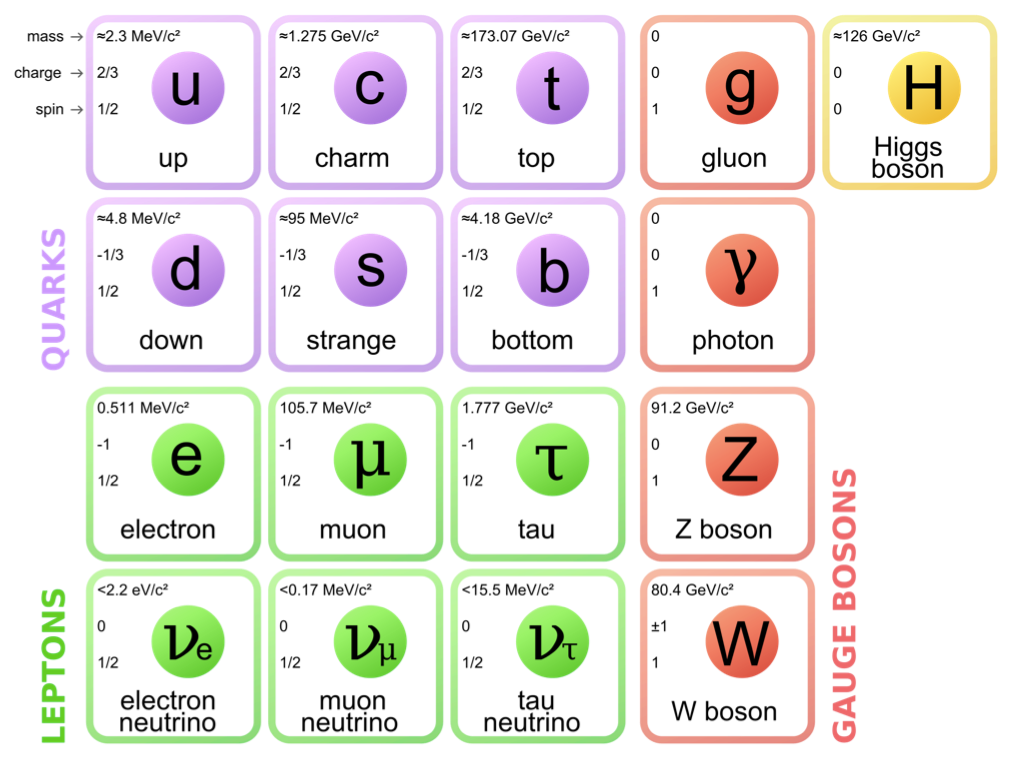
\includegraphics[width=0.8\textwidth]{Introduction/figs/SM.png}
\caption{A scheme of the fundamental particles in the SM with their properties~\cite{SM_particles}.}
\label{fig:SMparticles}
\end{figure}

Due to the asymptotic freedom of the strong interaction quarks cannot be observed in isolation and 
are always combined with other quarks to form color singlets~\cite{Gross:1973id}. Non-fundamental particles
composed of quarks are called hadrons and are classified into two groups: mesons, where the colour singlet
is achieved by the combination of a quark and an antiquark (\quark\quarkbar), and baryons
formed from three quarks (\quark\quark\quark) of different colours.
Recently, in 2014 and 2015 evidence for new states, formed by four and five quarks, was found~\cite{Aaij:2014jqa,Aaij:2015tga}.
%Recently evidence for particles composed by 4 quarks was also found~\cite{}.


\section{The electroweak interaction}
\label{sec:EMandEW}

The electromagnetic interaction is responsible for binding electrons and nuclei
together to form atoms and its mediator is the photon.
%
%,which also sets the range of the EM force to infinity, since this is proportional to the inverse of the mediator mass.
%In fact Heisenberg's Uncertainty Principle tells us that $\Delta E \Delta t > \hbar$, namely virtual particles
%of energy $\Delta E$ are allowed to exist for time intervals inferior to $\Delta t$. Thus, since particles can move
%at most at the speed of light, $c = 299792458$ ms$^{-1}$~\cite{PDG2014}, this also sets a relation between the length 
%of time and space in which a virtual photons can exist ($\Delta t > \hbar / (mc^2)$). As virtual photons can be very
%close to the mass shell, this results in a very long lifetime. The EM force has therefore an infinite range.
%
The weak interaction is responsible for the $\beta$ decay of nuclei and is mediated
by the exchange of $W^\pm$ and $Z^0$ bosons. Unlike the electromagnetic force,
that affects only charged particles, all known fermions interact through the weak interaction.
The weak interaction is also the only one that violates the parity symmetry, which states that interactions are invariant under
an inversion of spatial coordinates. This symmetry breaking arises from the fact that only left-handed fermions interact through
the weak interaction as discovered by Wu in 1957~\cite{Wu:1957my}. Similarly, the weak interaction
is the only one that also breaks the CP symmetry, which combines parity transformations and charge conjugation.
This is particularly interesting because all interactions are believed to be invariant under the CPT transformation, which combines the CP
transformation and time reversal. Hence, breaking CP the weak interaction implies that the process is also not invariant under 
time reversal transformations.

In 1968 Salam, Glashow and Weinberg unified the weak and electromagnetic forces into a single theory, where the coupling
constants of the electromagnetic, $e$, and weak, $g$, interactions are related through the weak mixing angle, $\theta_W$
by the relation $g\sin\theta_W = e$~\cite{PDG2014}. 
%
The electroweak symmetry is spontaneously broken by the Higgs
mechanism~\cite{Strocchi:1977za} and this causes the $W^\pm$ and \Z bosons to become massive (see Tab.~\ref{tab:interactions}) 
and consequently the weak force has a very short range. In fact, using Heisenberg's Principle, $\Delta E \Delta t > \hbar$, 
together with Einstein's formula $\Delta E = m c^2$, which relates mass and energy, and knowing that the maximum 
space that a particle can cover in a time $\Delta t$ is $r \sim c \Delta t$, qualitatively $r \sim \hbar / mc$. In this picture
the carriers of the weak force can travel $r \sim 2 \cdot 10^{-3}$~fm. In contrast, the photon must be massless in the theory, 
which accounts for the long range of the electromagnetic force.
%
The EW interactions are divided into Charged Currents (CC) and Neutral
Currents (NC). In the first group, quarks and leptons interact with the $W^\pm$ bosons, producing decays such as
$\mu^+(\mu^-) \rightarrow e^+ \nu_e \overline{\nu}_\mu (e^- \overline{\nu}_e \nu_\mu)$ and $n (\overline{n}) \rightarrow p e^- \overline{\nu}_e (\overline{p} e^+ \nu_e)$.
The study of these processes confirmed that only the left-handed (right-handed) component of fermions (anti-fermions)
takes part in weak processes. The CC interactions have a peculiarity: they are the only interactions in the SM that violate
flavour conservation at tree level, while any other interaction not conserving flavour has to proceed through
higher order processes. The second group of EW interactions, NC, corresponds to diagrams mediated by a photon or a \Z 
boson interacting with a fermion and its anti-fermion.



\section{Flavour and the CKM matrix}
\label{sec:flavour}

``Flavour" in particle physics refers to the quark/lepton composition of a particle. The introduction of flavour quantum numbers
was motivated in order to explain why some decays, although kinematically allowed, had never been observed. All leptons are
assigned a quantum number $L_\ell = 1$ (where $\ell = e,\mu,\tau$), which in the SM is conserved by all interactions.
This conservation is experimentally well established; for example decays like $\mu^- \rightarrow e^- \gamma $ have never
been observed.
%This is explained by the fact that the lepton number in the initial
%and final state are different and the decay would violate lepton flavour.
%
In the hadronic sector particles carry flavour numbers described as:
%
 \begin{itemize}
 \item \emph{Isospin}: $I_3 = 1/2$ for the up quark and $I_3 = -1/2$ for the down quark;
 \item \emph{Strangeness}: $S = -(n_s - \bar{n}_s)$, where $n_s$ and $\bar{n}_s$ are the numbers of strange
 and anti-strange quarks respectively;
 \item \emph{charmness, bottomness, topness}: in analogy to strangeness
 they are respectively defined as $C = -(n_c - \bar{n}_c)$, $B = -(n_b - \bar{n}_b)$, $T = -(n_t - \bar{n}_t)$.
 \end{itemize}

As mentioned previously, in the SM the only interaction violating flavour conservation is the weak interaction
when mediated by $W^\pm$ bosons.

Measuring branching fractions of weak decays such as $\pi \to \mu \nu_\mu$ and $K \to \mu \nu_\mu$, corresponding
respectively to $ud\to\mu\nu_\mu$ and $us\to\mu\nu_\mu$ processes, suggested the existence of more than one
coupling constant for different quarks. Nicola Cabibbo, in order to preserve the universality
of weak interactions, suggested that the differences could arise from the fact that
the doublets participating in the weak interactions are an admixture of the mass eigenstates~\cite{PDG2014,Cabibbo:1963yz}. 
He therefore introduced the Cabibbo angle, $\theta_c$, proposing that mass eigenstates participating 
in the weak interaction are rotated with respect to the flavour eigenstates.
%
\begin{equation}
\left( \begin{array}{c}
d_W \\ s_W
\end{array} \right) =
\left( \begin{array}{cc}
\cos \theta_c  & \sin \theta_c\\
-\sin \theta_c & \cos \theta_c
\end{array} \right)
\left( \begin{array}{c}
d \\ s
\end{array} \right) = 
\left( \begin{array}{c}
\cos\theta_c \cdot d + \sin \theta_c \cdot s \\
\cos \theta_c \cdot s - \sin \theta_c \cdot d
\end{array} \right)
\end{equation}

In a six quark system one angle is not sufficient to describe a rotation but the mixing can be generalised
using a $3 \times 3$ unitary matrix, called the CKM matrix, from the names of Cabibbo, Kobayashi and Maskawa~\cite{Cabibbo:1963yz,Kobayashi:1973fv}.
The unitarity of the matrix is required to preserve the universality of the weak interaction. Theoretically, a $N \times N$ complex
matrix depends on $2 \cdot N^2$ real parameters. Requiring unitarity ($AA^\dagger = A(A^*)^T = I$), the number
of independent parameters left is 
\begin{equation}
(N - 1)^2 = \underbrace{\frac{1}{2}N(N-1)}_\text{Number of mixing angles} + \underbrace{\frac{1}{2}(N-1)(N-2)}_\text{Number of complex phases}.
\end{equation}  
Therefore a $3 \times 3$ matrix depends then on 4 real parameters: three real constants 
and one imaginary phase. The imaginary phase generates the \mbox{CP-violation} which was
observed in weak interactions.
Figure~\ref{fig:ch_currents_ckm} displays examples of CC processes together with the CKM elements associated with their vertices.
%
\begin{figure}[h!]
\centering 
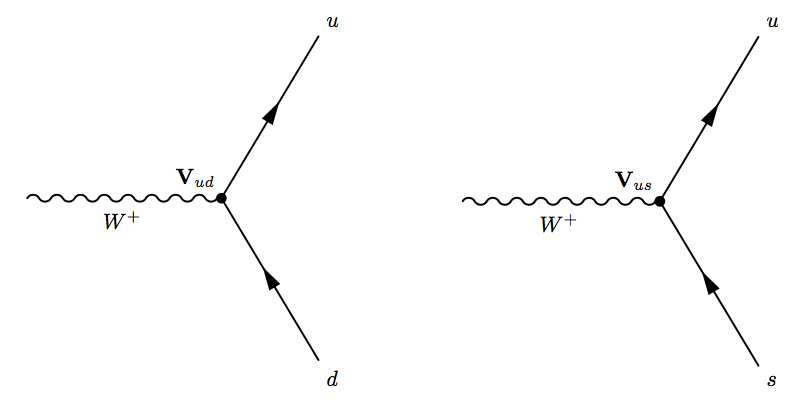
\includegraphics[width=0.6\textwidth]{Introduction/figs/ch_currents_ckm.png}
\caption{Feynman diagrams with CKM weights on weak interaction vertices as defined in Eq.~\ref{eq:CKM}.}
\label{fig:ch_currents_ckm}
\end{figure}
%
Equation~\ref{eq:CKM} reports the most recent measured values of its elements~\cite{PDG2014}
together with the widely used Wolfenstein parameterisation which highlights the hierarchical structure of the matrix.
In fact, elements on the diagonal, corresponding to transitions between quarks of the same generation,
are approximately 1 and become smaller and smaller going farther from the diagonal.
In the formula $\rho$, $A$, and $\lambda$ are the real constants and $\eta$ the imaginary phase 
and Eq.~\ref{params} shows how they are related to the three mixing angles; terms further from the diagonal 
are proportional to higher powers of $\lambda$.
%
\begin{eqnarray}
& V = \left( \begin{array}{ccc}
V_{ud} & V_{us} & V_{ub}  \\
V_{cd} & V_{cs} & V_{cb}  \\
V_{td} & V_{ts} & V_{tb}  
 \end{array} \right) = \left( \begin{array}{ccc}
0.9743 \pm 0.0002 & 0.2253 \pm 0.0007 & 0.0035^{+0.0002}_{-0.001} \\
 0.2252 \pm 0.0007 & 0.9734 \pm 0.0002 & 0.00412^{+0.0011}_{-0.0005} \\
 0.0087 \pm 0.0003 & 0.0404^{+0.0011}_{-0.0005} & 0.99915^{+0.00002}_{-0.00004} 
 \end{array} \right) \nonumber \\ [8pt]
& = \left( \begin{array}{ccc}
1 - \lambda^2/2 & \lambda  & A \lambda^3(\rho -i\eta) \\
-\lambda & 1 - \lambda^2/2 & A\lambda^2 \\
A \lambda^3(1 - \rho -i\eta) & A\lambda^2 & 1 
\end{array} \right) + O(\lambda^4)
\label{eq:CKM}
\end{eqnarray}
%
\begin{equation}
\begin{array}{rl}
\lambda & = \sin(\theta_{12}) = \sin(\theta_c) \\
A\lambda^2 & = \sin(\theta_{23}) \\
A\lambda^3(\rho - i\eta) & = \sin(\theta_{13})e^{i\delta}
\end{array}
\label{params}
\end{equation}
%
%
%Another feature to note is that, due to the unitarity of the matrix, the transformation has no effect on neutral interactions.
%
%In fact defining $q' = Vq$:
%
%\begin{equation}
%\bar{q}'q' = \bar{q}V^{*}Vq = \bar{q}q.
%\end{equation}
%
%As a result flavour-changing neutral currents are forbidden at tree level in the SM.
%

The unitarity of the CKM matrix imposes constraints to its elements of the form:
\begin{equation}
\sum_i |V_{ik}|^2 = 1 \text{ and } \sum_k V_{ik} V^{*}_{jk} = 0.
\end{equation}
These correspond to constraints on three complex numbers, which can be viewed
as the sides of triangles in the $(\rho,\eta)$ plane; these are called ``unitarity triangles".
The most commonly used unitarity triangle arises from $V_{ud}V^*_{ub} + V_{cd}V^*_{cb} + V_{td}V^*_{tb}=0$.
%\begin{equation}
%V_{ud}V^*_{ub} + V_{cd}V^*_{cb} + V_{td}V^*_{tb}=0.
%\end{equation}
Figure~\ref{fig:unitarity_triangle} shows a representation of such triangle together with
a plot summarising the most up-to-date experimental constraints to its parameters~\cite{Charles:2015gya}.
Due to these unitarity constraints flavour-changing neutral currents
are forbidden at tree level in the SM.

The precise measurement of the parameters of the CKM matrix
is a powerful stability test of the SM and sets a solid basis for new physics
searches in the flavour sector. One of the main goals of the LHCb experiment is to measure precisely
 the angle $\gamma$, which is currently the least constrained by measurements.
 %
\begin{figure}[h!]
\centering 
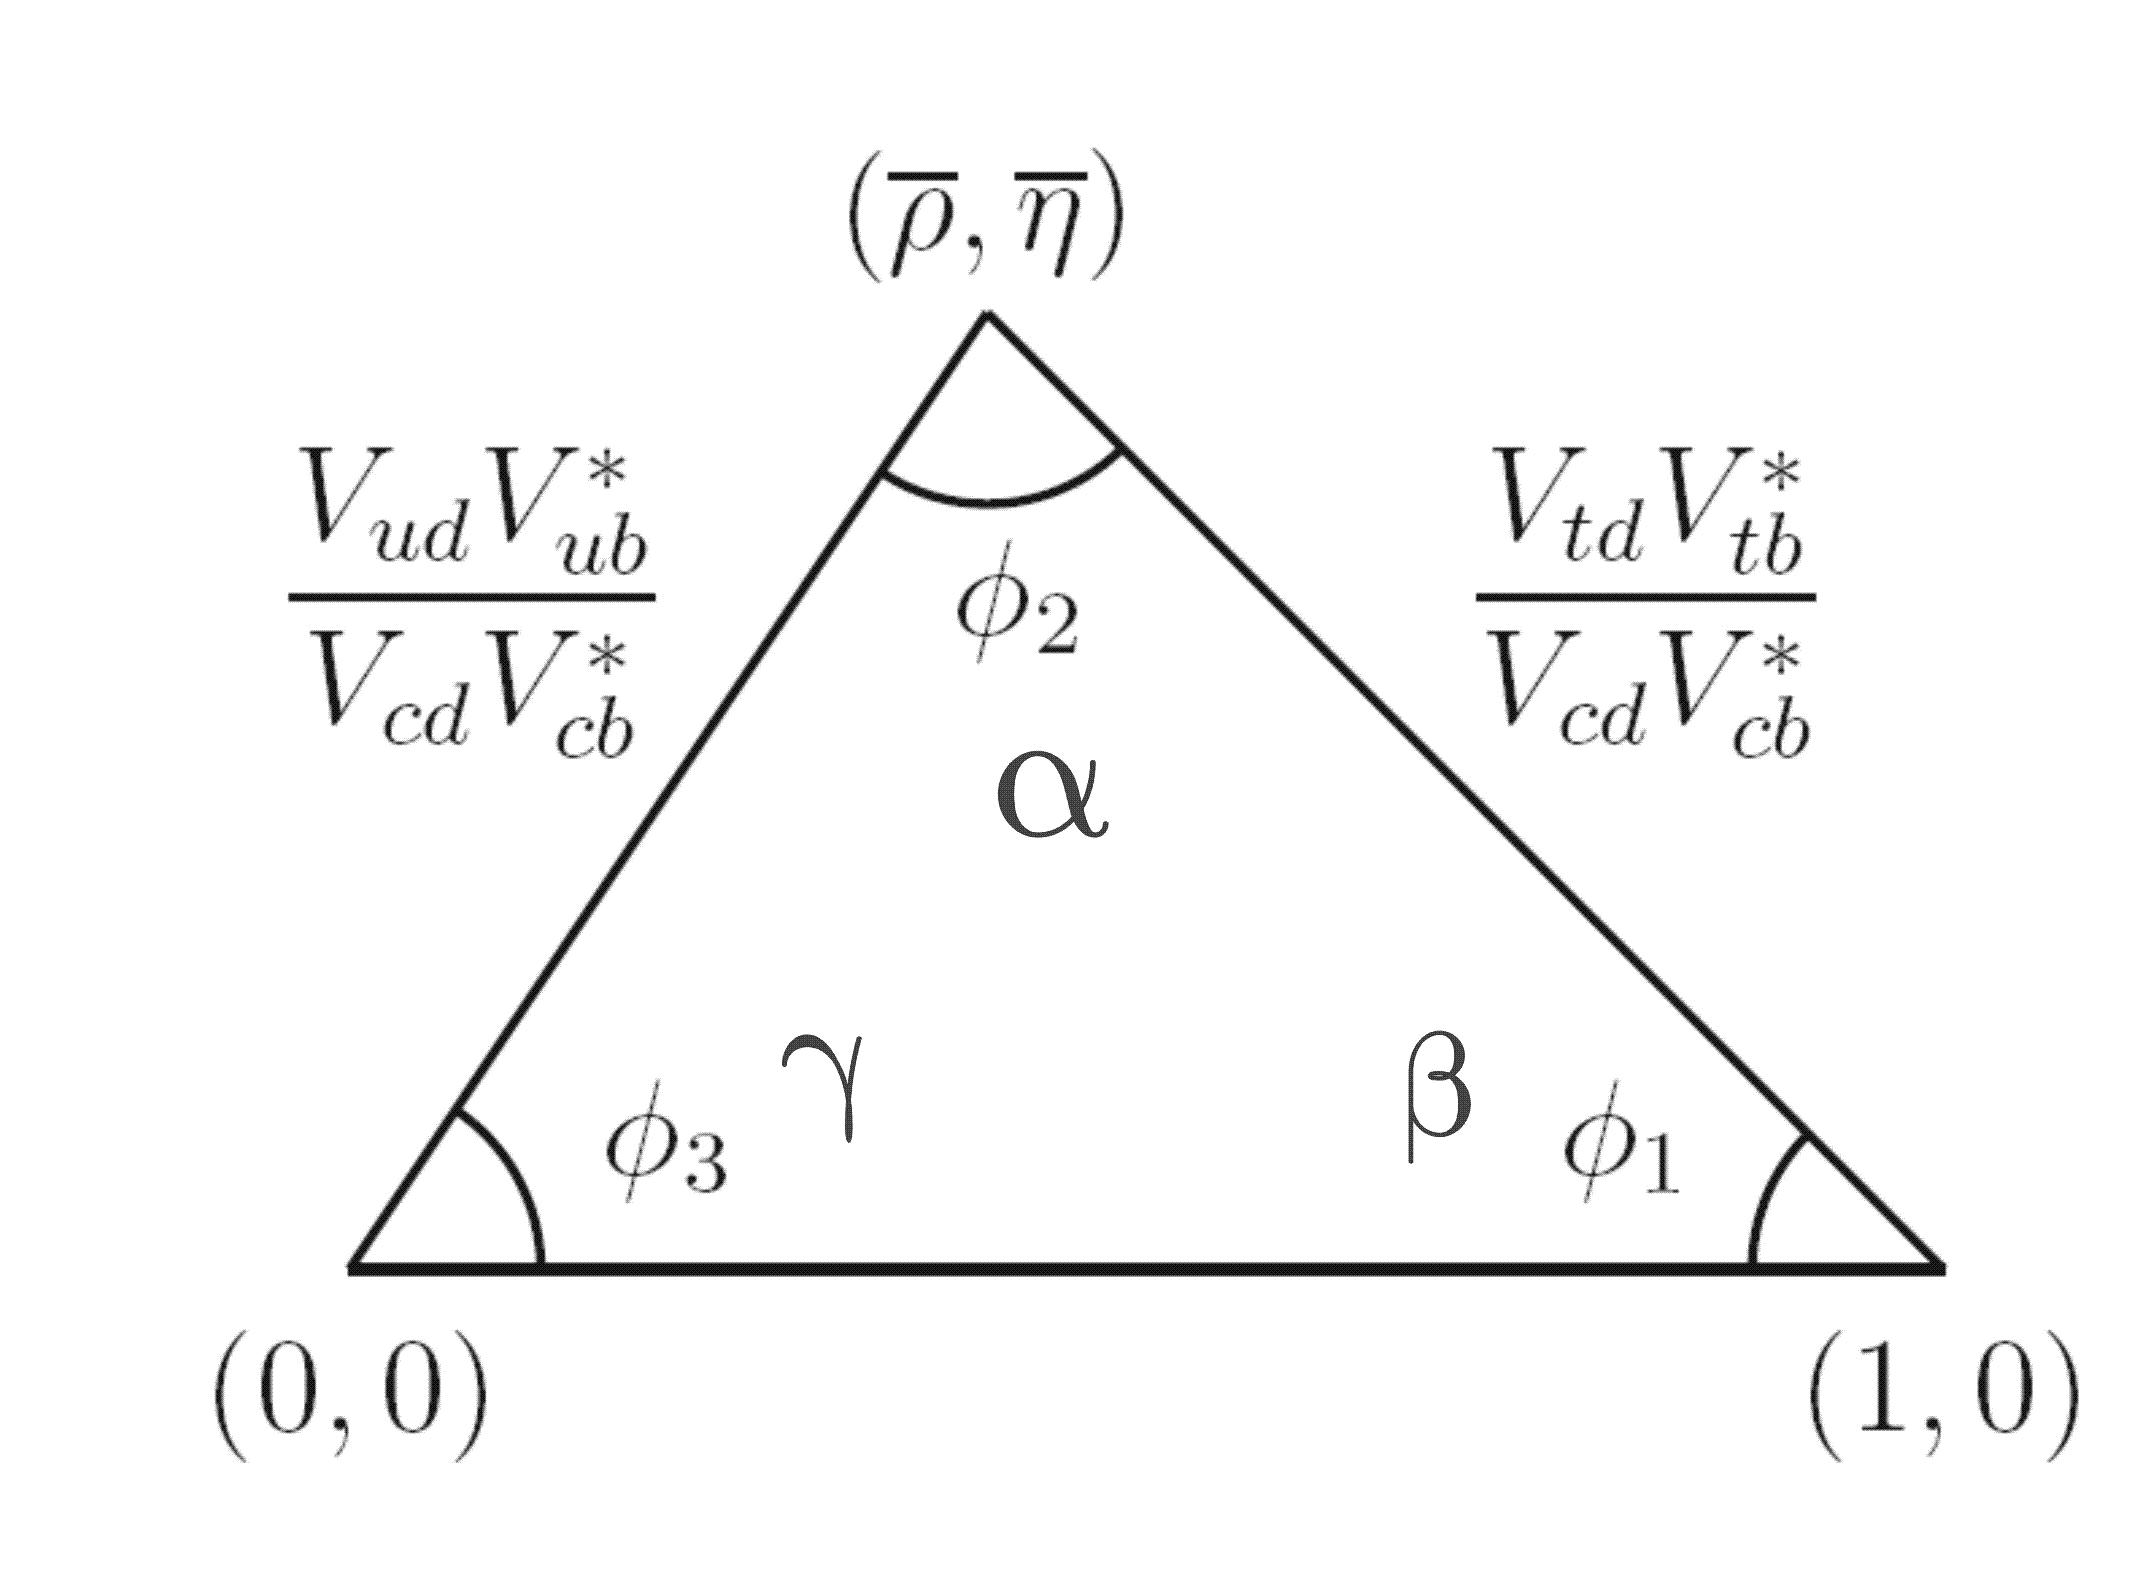
\includegraphics[width=0.5\textwidth]{Introduction/figs/Unitarity_triangle.png}
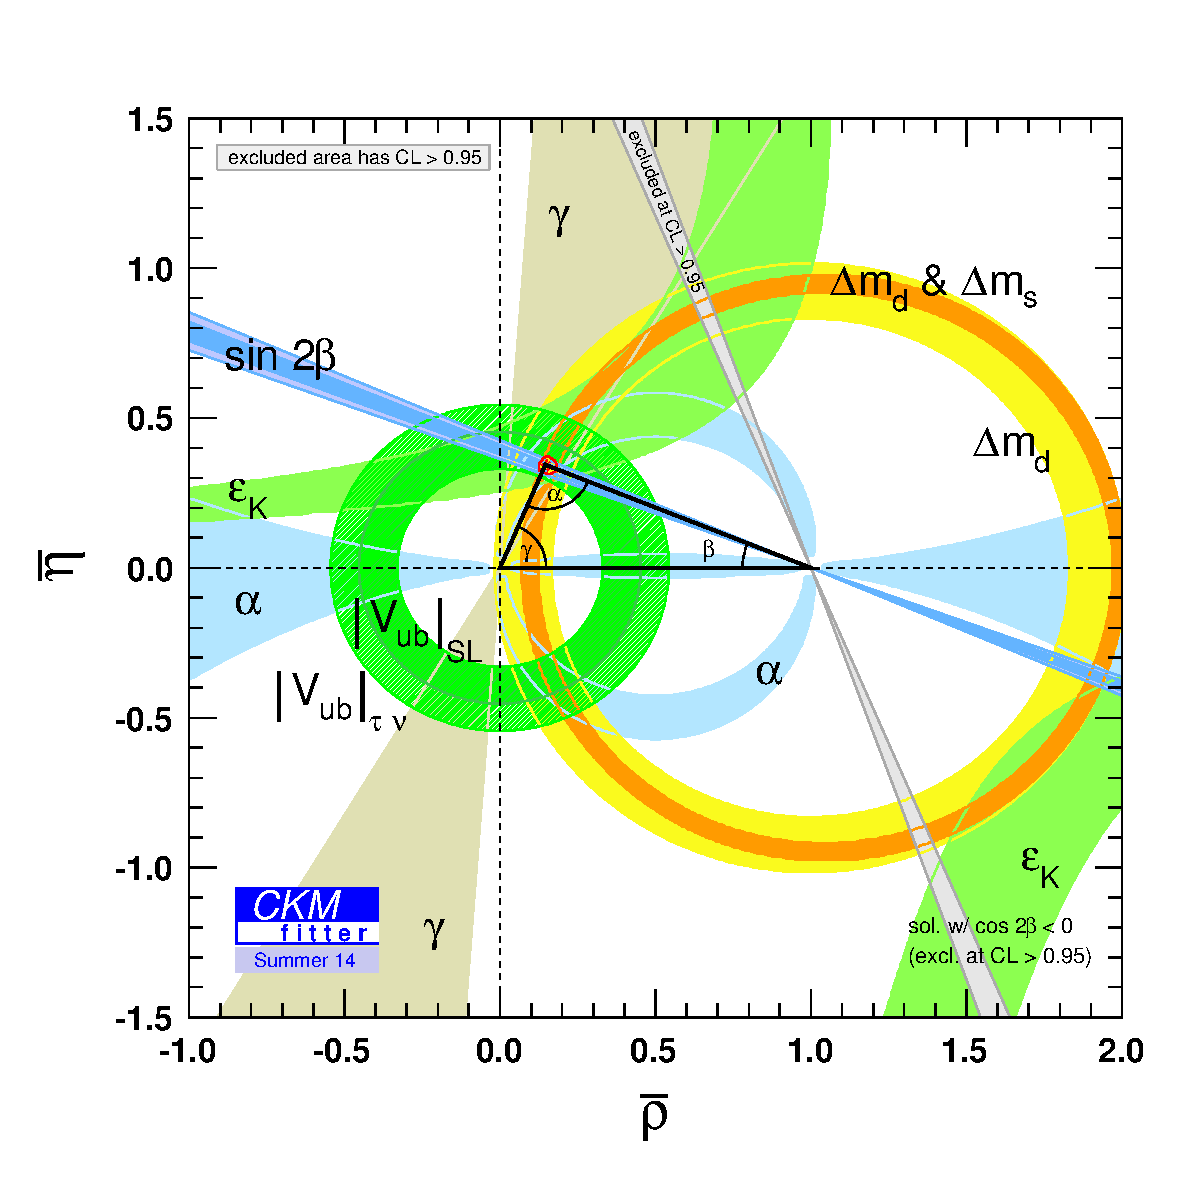
\includegraphics[width=0.7\textwidth]{Introduction/figs/Unitarity_triangle_HFAG.pdf}
\caption{(top) A representation of the unitarity triangle and its parameters.
(bottom) A summary of the most up-to-date measurements of the unitarity triangle parameters~\cite{Charles:2015gya}.}
\label{fig:unitarity_triangle}
\end{figure}
 
 
 
 
\section{The puzzles of the SM}
\label{sec:SMproblems}

Despite the experimental confirmation of many predictions of the SM, the theory has several limitations
and is unable to account for some well-established experimental facts:
%
\begin{itemize}
\item \emph{Dark matter}: experimental evidence tells us that the content of visible matter in the universe is not sufficient
to account for the observed rotation of galaxies~\cite{Zwicky:1933gu}. The most natural way to solve the problem
is the hypothesis of a form of matter that interacts with the gravitational field but not with the other SM interactions. 
%Furthermore, studies of the fluctuations of the cosmic microwave background indicate the existence of
%cold dark matter~\cite{Dunkley:2008ie}.
%formed of particles which do not interact through the SM forces and
%for which there is no SM candidate.
%
\item \emph{Matter-antimatter asymmetry}: a large asymmetry is observed between the quantity of matter 
and antimatter in the universe, $O(10^{-9})$. Assuming that both were equally created in the initial state of 
the universe, a condition such as the violation of the CP symmetry is necessary to account for the observed
imbalance. However, the magnitude of CP violation predicted by the SM, $O(10^{-20})$, is not sufficient to 
account for the observed asymmetry~\cite{Gavela:1993ts}.
%
\item \emph{Gravity}: even though the gravitational force was the first to be discovered 
this is not included in the SM. % as it can be neglected at the EW scale. 
When introducing gravity into the framework of QFT the
theory diverges. On the other hand gravity becomes irrelevant for the small masses 
of particles and can be neglected to a good approximation at the EW energy scale.
Many attempts have been made but there is not yet a consistent theoretical framework through which
 gravity can be introduced in the SM~\cite{Carlip:2001wq}. 
%
\item \emph{Neutrino oscillation}: measurements of solar and atmospheric neutrinos, as well as
neutrinos from nuclear reactors, have established that neutrinos can change flavour while propagating in space.
This is not predicted in the SM, in fact in the SM neutrinos are massless, while an oscillation requires a non-zero
 mass~\cite{Maltoni:2011zz,Cleveland:1998nv,Fukuda:1998mi,Eguchi:2002dm}.
%
\item \emph{The hierarchy problem}: the mass of a scalar (spin 0) particle, such as the Higgs boson,
suffers from quantum corrections due to the physics at high energy scales. As new physics can appear
anywhere up to the Planck scale, $\sim 10^{19}$~\gev, at which gravity cannot be neglected any more,
these corrections can be very large and it would require a high level of fine-tuning for them to cancel 
out and give such a small value as the one measured for the
Higgs Mass, $\sim 126$~\gevcc~\cite{Feng:2013pwa,Aad:2012tfa}. 
%This is considered unnatural by many physicists and pushes them
%to look for further motivations.
%
\end{itemize}
%
In conclusion, even though the SM has been very successful in describing the properties of the observed particles
and their interactions so far, because of its many puzzles, it is believed only to be part of a more general theory 
or only to be valid up to a certain energy scale. %Many theoretical models expect New Physics (NP) to enter at the TeV scale.

\subsection{The flavour problem}

%As mentioned in Sec.~\ref{sec:flavour}, flavour conservation is well experimentally established but it does not
%have a strong theoretical otivation in the Standard Model.
Flavour Changing Charged Currents (FCCC) that are mediated by the $W^\pm$ bosons are the only sources of flavour changing interactions 
in the SM and, in particular, of generation changing interactions, where a quark or a lepton of a family transforms
into one of an other family. Another class of processes is the Flavour Changing Neutral Currents (FCNCs), \emph{e.g.} transitions from a
\bquark quark with a charge of -1/3 to a \squark or \dquark quark with the same charge. Examples of FCNC transitions in the quark
and lepton sector are shown in Fig.~\ref{fig:neutr_curr}.
%
\begin{figure}[h!]
\centering 
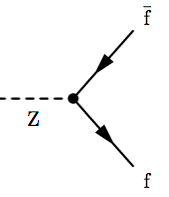
\includegraphics[width=0.25\textwidth]{Introduction/figs/Z2ffbar.png}
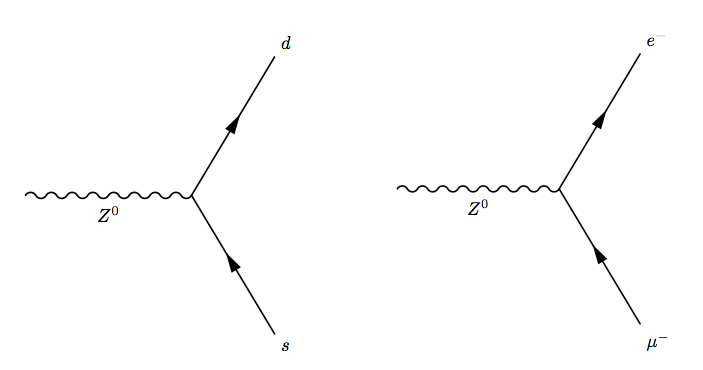
\includegraphics[width=0.6\textwidth]{Introduction/figs/neutral_current_proc.png}
\caption{Feynman diagrams of a neutral current allowed in the SM (left), where$f$ represents any fermion,
and FCNCs processes forbidden in the SM (center-right).}
\label{fig:neutr_curr}
\end{figure}
%
FCNCs are experimentally observed to be highly suppressed which derives from the unitarity of the CKM matrix,
however there is no fundamental reason why there cannot be FCNCs at tree level. In fact the CKM matrix
could be part of a larger matrix involving for example quark-lepton terms. This would introduce
new sources of FCNCs but could also allow for natural explanations of the equality of the proton and electron charges.
Furthermore, the observation of neutrino oscillation proves that flavour is not always conserved
suggesting flavour structures beyond the SM. Finally, the values of the terms of the CKM matrix and the PMNS
matrix~\cite{Pontecorvo:1967fh,Maki:1962mu}, which is the mixing-matrix equivalent to the CKM in the lepton sector,
are not explained in the SM but have to be measured experimentally. These open problems motivate searches for flavour
symmetries and deeper motivations for flavour conservation. 

\section{Beyond the Standard Model}

From the previous sections it is evident that, despite the great success of the SM, there is a need to explore theories Beyond the SM (BSM).
Among the most promising approaches there are those involving Super-Symmetry (SUSY)~\cite{Fayet:1976cr} and extra-dimensions~\cite{Randall:1999ee}. 
%
In SUSY new degrees of freedom are introduced to suppress the diverging terms of the Higgs mass. This theory
assumes that for each fermion there is a corresponding boson and, since bosons and fermions contribute with opposite
sign to the mass term, these would naturally cancel out. Super-Symmetry also provides a candidate for dark
matter. In fact the lightest Super-Symmetric particle, the neutralino, which in R-parity~\cite{Ellis:1984gi} conserving 
variants of the theory must be stable, is a weakly interacting and potentially massive particle.
%
The idea to introduce extra-dimensions was triggered by the fact that gravity is not relevant in particle physics but it would 
be natural if all forces had similar strength. By adding extra dimensions to the normal three spatial dimensions, one can restore 
the strength of gravity, as this could be dispersed by the wider space available.
%
In all these approaches, constraints to masses and couplings must be imposed to maintain
compatibility with the SM at the electroweak scale and the existing experimental observations.

\subsection{Flavour and BSM theories}

Most BSM theories predict processes violating flavour conservation. Therefore, the observation or
non-observation of these processes can give important information about new physics.
BSM theories can be classified according to the amount of flavour violation they introduce.
The first class of models to consider is that with Minimal Flavour Violation (MFV).
These are models in which the only sources of flavour changing transitions are governed by the
CKM matrix and the CKM phase is the only source of CP violation.
This definition is driven by the fact that usually a solution of the hierarchy problem is expected
at the TeV scale, while the very small amount of flavour violation observed in measurements
seems to indicate that the SM would remain valid up to much higher energy scales.
It is therefore assumed that new physics must respect flavour symmetry principles, which also makes these
types of models naturally compatible with the SM. Examples of such models include the MSSM
with minimal flavour violation and the SM with one extra-dimension. Reviews of MFV models
are presented in Refs.~\cite{Isidori:2012ts,Buras:2003jf}.
%
%The MFV hypothesis provides a way to resolve the tension between expectation, driven by naturalness arguments,
%that NP should be at the \tev~scale and limits on FCNC processes that point to much higher scales.
%
A powerful test of MFV is provided by the study of ratios between $\bquark\to\dquark$ and $\bquark\to\squark$
transitions, because their Hamiltonians share the same structure. One particularly important example is the ratio between the 
decay rates of $\Bz$ and $\Bs$ into dimuons~\cite{TomRDreview}, as this is a purely leptonic decay free from hadronic uncertainties.
In the SM such ratios are approximately equal to $|V_{td}/V_{td}| \sim 1/25$, only modified by phase space and hadronic
matrix elements, while they can take very different values in non-MFV models.

In the quest for new physics an important role is also played by simplified models
as an intermediate model building step. Instead of constructing theories valid up to the GUT scale
one can consider simplified models, where the SM is extended by the addition of new degrees of freedom
with a limited number of parameters. Such models are easier to constrain but can nevertheless point
in the right direction to build more complete theories. The choice of the new sector to add can be driven 
by the need to explain existing tensions between measurements and SM predictions or by theoretical prejudice.
%
Two models especially relevant when studying rare decays, which are the main topic of this thesis, are 
$Z'$-penguins and leptoquarks. A $Z'$-penguin is a FCNC process involving a neutral field arising from an extra 
U(1) gauge symmetry, for example U(1)$_{B-L}$, where $B$ and $L$ are the baryon and lepton numbers. 
As for the SM penguins, the $Z'$ field contributes in loops causing modifications of the 
effective couplings with respect to the SM. A survey of $Z'$ models can be found in Ref.~\cite{Buras:2014zga}.
%
Leptoquarks are bosonic particles that carry both quark and lepton flavour quantum numbers, which
for simplicity are assumed to be scalar.
A tree level exchange of a leptoquark induces processes such as $\bquark \to (\squark,\dquark)\ell^+\ell^-$,
and therefore can result in an enhancement of their decay rates with respect to the SM~\cite{Hiller:2014yaa}.
Leptoquarks would also provide a natural explanation for non-universal couplings to leptons.


\section{Rare decays: a tool to search for new physics}
\label{sec:RD_theory}

In the Standard Model FCNC processes are forbidden at tree level but
can occur through loop diagrams such as penguin or \W box diagrams (see Fig.~\ref{fig:penguins}).
The branching fractions of decays going through these processes are small, typically \mbox{$\sim10^{-6}$} 
or lower, and therefore they are called ``rare decays". Additional contributions to the virtual loops
are not necessarily suppressed with respect to the SM component which makes these decays
very sensitive to new physics. This approach to new physics searches is interesting as
new particles could be at high mass scales that are not accessible via direct production at colliders
but their effect could be observed in loops.
Radiative and penguin decays are particularly interesting because they are theoretically
well understood, which allows precise comparisons with measurements. Furthermore, they provide
a large quantity of observables that can be affected by new physics, not only decay rates, but also 
CP asymmetries and angular observables such as forward-backward asymmetries. The joint
analysis of different observables can help to build a consistent picture and rule out specific models.
%
\begin{figure}[h!]
\centering
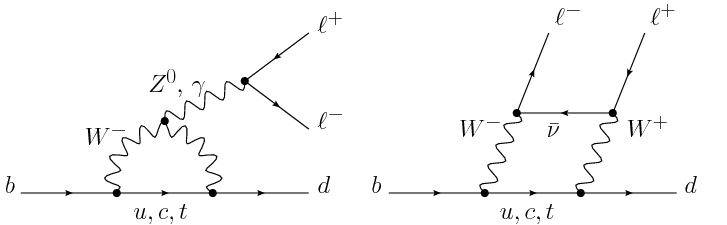
\includegraphics[width=0.9\textwidth]{Introduction/figs/penguin_general.png}
\caption{Loop Feynmann diagrams allowing $\bquark \to \dquark$ FCNC 
processes: penguin diagram (left) and \W box (right).}
\label{fig:penguins}
\end{figure}

\subsection{Theoretical framework: the effective Hamiltonian}
\label{sec:Effective_Hamiltonian}

Rare decays of \bquark hadrons are governed by an interplay between weak
and strong interactions.
%The QCD corrections that arise from hard gluon exchange bring large logarithms
%of the form $\alpha_s^n(m_b)\log^m(m_b/M)$, where $M = m_t$ or $M = m_W$.
%A suitable framework to achieve the necessary resummation of these logarithms
%in an effective low-energy theory with five quarks.
%The QCD corrections that arise from hard gluon exchange bring large contributions
%large logarithms of the form $\alpha_s^n(m_b)\log^m(m_b/M)$, where $M = m_t$ or $M = m_W$.
The large masses of the $W^\pm$ and $Z^0$ bosons and top quark compared to that of the \bquark quark allow
the construction of an effective theory that divides the problem of calculating
weak decay amplitudes into two parts: ``short-distance" and ``long-distance" effects separated
at an energy scale $\mu$. The first part, dealing with short distance physics, handles
perturbative contributions due to energy scales above the \bquark mass. The second part
typically deals with non-perturbative contributions. 
A classic example of an effective theory is the Fermi theory of weak interactions
which describes the $\beta$ decay in terms of a four-fermion interaction,
where the short distance physics is hidden into a point-like vertex as illustrated in Fig.~\ref{fig:fermi_theory}.
\begin{figure}[h!]
\centering
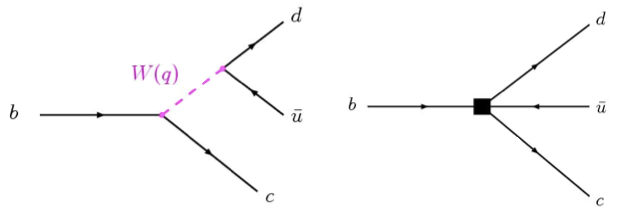
\includegraphics[width=0.7\textwidth]{Introduction/figs/fermi_theory.png}
\caption{Example of a Fermi theory in which the full theory (left) is divided into (right) a
short distance contribution, hidden in the vertex, and a long distance contribution.}
\label{fig:fermi_theory}
\end{figure}
\clearpage
The effective Hamiltonian~\cite{Chetyrkin:1996vx} relevant to
$\bquark\to\squark/\dquark \gamma$ and  $\bquark\to\squark/\dquark \ell^+\ell^-$
transitions can be written as:
%
\begin{equation}
\mathcal{H}_{eff} = \frac{-4G_F}{\sqrt{2}} \left[ \lambda^t_q \sum C_i(\mu,M)\mathcal{O}_i(\mu)
+ \lambda^u_q \sum C_i(\mu,M)(\mathcal{O}_i(\mu) - \mathcal{O}_i^u(\mu)) \right],
\end{equation}
%
where $G_F$ denotes the Fermi coupling constant and the $\lambda$ constants are the CKM factors,  
$\lambda^t_q = V_{tb}V_{tq}^*$ and  $\lambda^u_q = V_{ub}V_{uq}^*$. In $\bquark\to\squark$ quark transitions, 
which are the main topic of this thesis, the doubly Cabibbo-suppressed contributions can be neglected as 
$\lambda^u_s << \lambda^t_s$. To obtain this formula the Operator Product Expansion (OPE)~\cite{Buchalla:1995vs} method
is used, which implements a summation over all contributing operators weighted by corresponding constants
called Wilson coefficients. In this Hamiltonian the long-distance contributions are described by the 
operators, $\mathcal{O}_i$, while the short-distance physics is encoded in the Wilson 
coefficients, $C_i$. Operators and coefficients are evaluated at the renormalisation scale $\mu$.
Any particle that contributes to the decay and has a mass greater than the scale $\mu$ will affect the value 
of at least one of the Wilson coefficients, including SM particles as the top quark.

In order to describe SM processes the effective theory must be matched with the SM by requiring 
the equality between each term in effective theory and the full theoretical calculation at a matching 
scale, typically the EW scale ($\mu_W$). Then, using the scale independence of the
effective Hamiltonian, one can derive a renormalisation group equation for the Wilson coefficients~\cite{Buras:1998raa}.
%
%
%\begin{equation}
%\mu \frac{\deriv}{\deriv \mu} C_i(\mu) = \gamma_{ij}C_j(\mu),
%\end{equation}
%
%where the matrix $\gamma$ is the anomalous dimensions matrix of the operators $\mathcal{O}_i$.
%At leading order the solution is given by~\cite{Buras:1998raa}:
%
%\begin{equation}
%C_i(\mu) = \left[ \frac{\alpha_s(\mu_W)}{\alpha_s(\mu)}\right]^{\frac{\gamma^0_{ii}}{2\beta_0}} C_i(\mu_W) = \left[ \frac{1}{1 + \beta_0\frac{\alpha_s(\mu)}{4\pi}ln\frac{\mu_W^2}{\mu^2}} \right]^{\frac{\gamma^0_{ii}}{2\beta_0}} C_i(\mu_W),
%\end{equation}
%
%where $\alpha_s$ is the strong coupling constant.
%
Taking into account only SM contributions and using $\mu_W = m_b$, the Wilson coefficients have values:
%
\begin{equation}
\begin{array}{ccc}
C_7^{SM} = -0.3, & C_9^{SM} = 4.2, & C_{10}^{SM} = -4.2
\end{array}
\end{equation}
%
and new physics contributions appear in the Wilson coefficients in the form of additive factors:
\begin{equation}
 C_i = C_i^{NP} + C_i^{SM}.
\end{equation}

The amplitudes of exclusive hadronic decays can be calculated as the expectation 
values of the effective Hamiltonian. Given an initial state $I$ and a final state $F$
\mbox{(\emph{e.g.}: $I = \Bz$ and $F=\Kstarz\mumu$)} the decay amplitude can be calculated as
%
\begin{equation}
\begin{array}{rl}
A(I\to F) &= \langle I | \mathcal{H}_{eff} | F \rangle = \\
&= \frac{G_F}{\sqrt{2}} \sum V_{CKM}^i \underbrace{C_i(\mu)}_{\shortstack{Perturbative \\ Includes new physics}} \cdot  \underbrace{\langle I | \mathcal{O}_i(\mu) | F \rangle}_{\shortstack{Non-preturbative \\ Known physics}},
\end{array}
\end{equation}
where $\langle I | \mathcal{O}_i(\mu) | F \rangle$ are the hadronic matrix elements also called  ``form factors".
These can be evaluated using non perturbative methods such as lattice calculations.
However, due to the limitations of these methods, they represent the dominant source 
of uncertainty in theoretical calculations.

\subsection{Operators}
\label{sec:operators}

Separating the left- and right-handed components the effective Hamiltonian is
%for $\bquark\to\squark\ell^+\ell^-$ transitions is
%
\begin{equation}
\mathcal{H}_{eff} = \frac{4G_F}{\sqrt{2}} V_{tb}V^*_{ts} \frac{\alpha_e}{4\pi} \sum_{i=1}^{10} \left[ C_i \mathcal{O}_i  +  C'_i \mathcal{O}'_i \right].
\end{equation}
%
%where the $V_{ub}$ and $V_{bs}$ are the factors of the CKM matrix.
A complete basis is given by a set of 10 operators, where $\mathcal{O}_{1,2}$ are the tree level W operators;
$\mathcal{O}_{3-6,8}$ are penguin diagrams mediated by gluons; and $\mathcal{O}_{7,9,10}$, which are the operators
that are relevant for radiative and leptonic penguin processes are defined as~\cite{TomRDreview}:
%S is Higgs scalar penguins and P pseudo-scalar penguin
%
\begin{equation}
\begin{array}{ll}
 \mathcal{O}_7 = \frac{m_b}{e} (\bar{s} \sigma^{\mu\nu}P_Rb)F_{\mu\nu},  		& \mathcal{O}_7' = \frac{m_b}{e} (\bar{s} \sigma^{\mu\nu}P_Lb)F_{\mu\nu}, \\
%\mathcal{O}_8 = g_s\frac{m_b}{e} (\bar{s} \sigma^{\mu\nu}P_RT^ab)G^a_{\mu\nu}  	& \mathcal{O}_8' = g_s\frac{m_b}{e} (\bar{s} \sigma^{\mu\nu}P_LT^ab)G^a_{\mu\nu} \\
\mathcal{O}_9 = (\bar{s} \gamma_{\mu}P_Lb)(\bar{\ell}\gamma^\mu\ell), 			& \mathcal{O}_9' = (\bar{s} \gamma_{\mu}P_Rb)(\bar{\ell}\gamma^\mu\ell), \\
\mathcal{O}_{10} = (\bar{s} \gamma_{\mu}P_Lb)(\bar{\ell}\gamma^\mu\gamma_5\ell), 	& \mathcal{O}_{10}' = (\bar{s} \gamma_{\mu}P_Rb)(\bar{\ell}\gamma^\mu\gamma_5\ell),
\end{array}
\end{equation}
%
where $P_{L/R} = (1 \mp \gamma_5)/2$ denote the left- and right-handed chiral projections 
%$T^a$ are the QCD generators 
and $F_{\mu\nu}$ is the electromagnetic field tensor.
%
The $\mathcal{O}'$ operators correspond to right-handed coupling obtained by swapping
$P_R$ and $P_L$ in the equations. In the SM, as well as in MFV models where the
flavour violation is entirely ruled by the CKM matrix, the $C'$ Wilson coefficients 
are suppressed by the strange coupling, $C'_i \sim (m_s / m_b) C_i$.
%
The operator $\mathcal{O}_7$ relates to penguin diagrams that are mediated via a photon.
%and the $\mathcal{O}_8$ by a gluon. The $\mathcal{O}_7$ operator is 
It represents the dominant contribution to the radiative 
$\bquark\to\squark\gamma$ transition and contributes to $\bquark\to\squark\ell^+\ell^-$ processes when
the virtual photon decays into a dilepton pair. The semileptonic $\mathcal{O}_9$ and $ \mathcal{O}_{10}$ 
correspond to penguin diagrams mediated by a $Z^0$ boson and $W$ mediated box diagrams. 
These are the dominant contributions in semileptonic $\bquark\to\squark\ell^+\ell^-$ decays.
The vertices corresponding to the radiative and semileptonic operators are illustrated in Fig.~\ref{fig:vtx_operators}
%
\begin{figure}[h!]
\centering
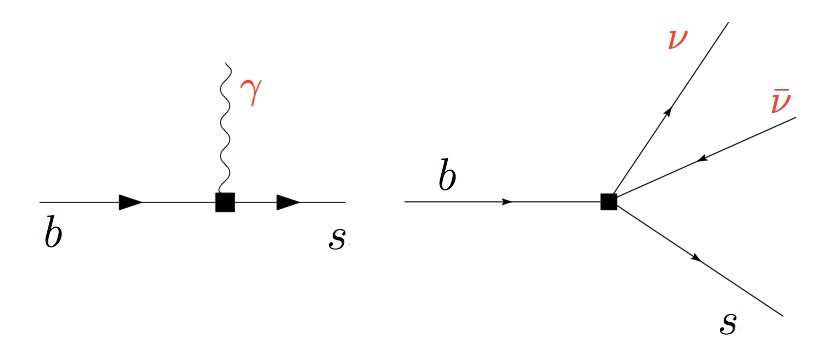
\includegraphics[width=0.6\textwidth]{Introduction/figs/vtx_operators.png}
\caption{Interaction vertices corresponding to the radiative (left) and semileptonic (right) operators.}
\label{fig:vtx_operators}
\end{figure}

It is also common to express the semileptonic operators in a basis with left and right projected leptons
%
\begin{equation}
\begin{array}{ll}
\mathcal{O}_{LL} = ( \mathcal{O}_{9} - \mathcal{O}_{10})/2 & \mathcal{O}_{LR} = ( \mathcal{O}_{9} + \mathcal{O}_{10})/2 \\
\mathcal{O}_{RR} = ( \mathcal{O}'_{9} - \mathcal{O}'_{10})/2 & \mathcal{O}'_{RL} = ( \mathcal{O}'_{9} + \mathcal{O}'_{10})/2 \\
\end{array}
\end{equation}
%
where the Wilson coefficients are redefined as
\begin{equation}
\begin{array}{ll}
C_{LL} = C_{9} - C_{10}, & C_{LR} =  C_{9} + C_{10}, \\
C_{RR} = C'_{9} - C'_{10}, &C'_{RL} =  C'_{9} +C_{10}. \\
\end{array}
\end{equation}
%
This basis is particularly useful in frameworks where BSM physics at a high mass scale
respects the SU(2)$_W$ part of the SM gauge symmetry group.
%For instance, instead of fitting the two parameters $C_9$
%and $C_{10}$, the LL-hypothesis gives the constraint $C_9 + C_{10} = 0$.
%since C9 +C10 = 0 in the standard model there is no sensitivity to CLR and 
%CRR from interference with the standard model in semileptonic decays.
%
Finally, in the picture presented in this section all operators were considered as universal
with respect to the flavour of the involved leptons. However, BSM models often contain sources of
lepton universality violation leading to a split of the same operators depending on the lepton considered:
$C_i \to C_i^e$, $C_i^\mu$, $C_i^\tau$ and $\mathcal{O}_i \to \mathcal{O}_i^e$, $\mathcal{O}_i^\mu$, $\mathcal{O}_i^\tau$. 

\subsection{Phenomenology of $\bquark\to\squark\ell^+\ell^-$ decays}
\label{sec:theo_qsq}

Semileptonic \bquark hadron decays are characterised by two kinematic regimes which
are treated theoretically in different ways; Table~\ref{tab:q2scheme} shows a scheme of the \qsq spectrum.
%
The ``high $q^2$" is the region of low hadron recoil, $\qsq > 15$~\gevgevcccc, and is characterised by 
the energy of the hadron being less than the energy scale of QCD interactions within the meson, 
\mbox{$\Lambda_{QCD} \sim 1$~\gev}. In this region theoretical calculations of $B$ meson decays can be simplified 
by working in the heavy quark limit, $m_b\to\infty$. In this limit a Heavy Quark Effective 
Theory (HQET) can be constructed~\cite{DellaMorte:2015yda} in which the heavy quark interacts 
only via `soft' hadronic processes and an OPE in $1/m_b$ is valid.
%?QCD/mb then shows that the perturbatively calculable parton-level process is the leading 
%contribution to the B0 ?K?0?+?? decay, and the hadronic effects are relatively small. 
%. A heavy-quark expansion in terms of The QCD Factori- sation (QCDF) technique separates the parton-level and %hadronic contributions at the energy scale ??mb, accounting for the ?soft? non-perturbative processes using hadronic %form factors [25].
%
%
%\begin{table}[b]
%\caption{A scheme of the \qsq spectrum.}
%\begin{tabular}{llcrr}
%{\footnotesize $\qsq = 0$ }   &  {\footnotesize  $E_{\Kstarz}  >> \Lambda_{QCD}$	}&  {\footnotesize $\qsq \sim m_{\jpsi,\psitwos}^2$ } & {\footnotesize $E_{\Kstarz}  \sim \Lambda_{QCD}$ } & {\footnotesize $\qsq = (m_B - m_\Kstarz)^2$ } \\
%\hline
%{\footnotesize max. recoil } & {\footnotesize large recoil (SCET) } & {\footnotesize $\cquark\cquarkbar$ resonances } & {\footnotesize low recoil (HQET) } & {\footnotesize zero recoil} \\
%\end{tabular}
%\label{tab:q2scheme}
%\end{table}
\begin{table}[b]
\caption{A scheme of the \qsq spectrum.}
\centering
\begin{tabular}{c|c|c|c}
 \qsq							& $E_{\Kstarz}$	   	&  	Regime 			& 	Valid theory \\ \hline
 $\sim 0$ \gevgevcccc			& $\sim m_B$			&   Max. recoil			&	\multirow{ 2}{*}{SCET}\\ 
 $< 6$	\gevgevcccc			& $>> \Lambda_{QCD}$	&	Large recoil		&		   		\\ \hline
 $\qsq \sim m_{\jpsi,\psitwos}^2$ 	& $\sim 3$ \gev			& 	$\cquark\cquarkbar$ resonances	&  -- 		\\ \hline
 $\qsq > 15$ \gevgevcccc 			& $E_{\Kstarz}  \sim \Lambda_{QCD}$ 			&	Low recoil	&	\multirow{ 2}{*}{HQET}\\
 $\qsq = (m_B - m_\Kstarz)^2$ 		& $E_{\Kstarz} \sim 0$  	&	Zero recoil		&			\\
\end{tabular}
\label{tab:q2scheme}
\end{table}
%
The \mbox{``low $q^2$"} region is where the light spectator quark is energetic and cannot be neglected.
Furthermore, the light quark interacts not only via `soft' hadronic processes, as in HQET, but also via the 
so-called `collinear' hadronic processes.
The boundary of this region can be set at $\sim 7$~\gevgevcccc~ which corresponds to the threshold for 
$\cquark\cquarkbar$ production, $(2m_c)^2$. 
In this region the hadronic interactions are handled by expanding in terms 
of the energy of the emitted energetic hadron, $1/E_h$, forming the so-called Soft-Collinear 
Effective Theory (SCET)~\cite{Bauer:2000yr}.
%
\begin{figure}[h!]
\centering
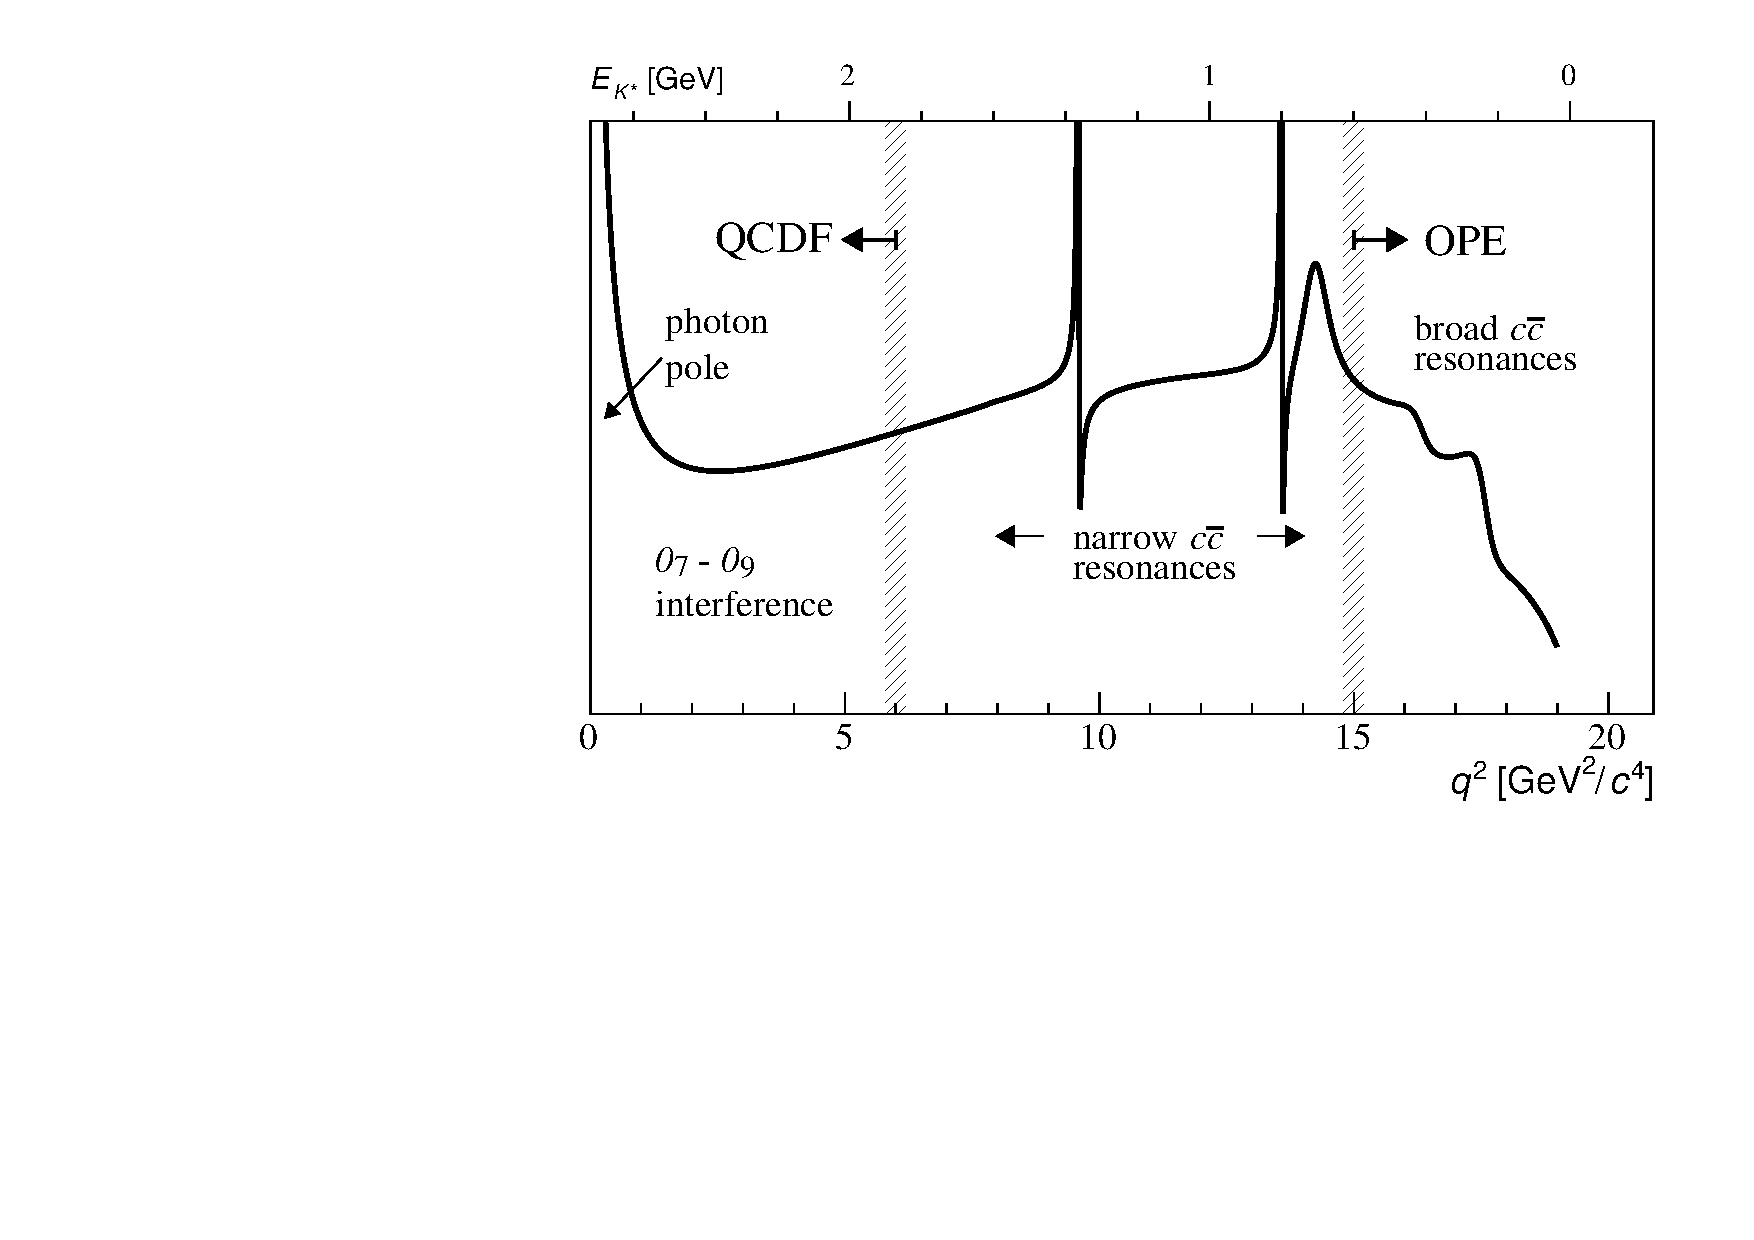
\includegraphics[width=0.8\textwidth]{Introduction/figs/q2spectrum.pdf}
\caption{A typical \qsq spectrum of $\bquark\to\squark\ll$ processes characterised by the photon pole
at  low \qsq, charmonium resonances at central \qsq and broad resonances at high \qsq~\cite{TomRDreview}.}
\label{fig:q2spectrum}
\end{figure}
%
In both regions decay rates can be predicted using the different methods and
the biggest uncertainties come from the limited knowledge of hadronic transition matrix elements.
The intermediate region is characterised by the presence of charmonium resonances, produced though tree 
level $b\to\cbar c s$ transitions and no precise theoretical calculation is available~\cite{Khodjamirian:2010vf}.

As can be seen in Fig.~\ref{fig:q2spectrum} the very low \qsq region is characterised by a peak due
to the virtual photon contribution, associated with $C_7$. In the region $1-6$~\gevgevcccc the 
interference between $C_7$ and $C_9$ becomes large, yielding sensitivity to new physics in $C_9$.
The $7-15$~\gevgevcccc interval is dominated by the charmonium resonances, \jpsi and \psitwos. 
Although these decays can be experimentally vetoed, in
principle charmonia affect the entire \qsq space. Finally, at high \qsq broad charmonium resonances 
can contribute, like those observed by LHCb in $\decay{B^+}{K^+\mumu}$ decays~\cite{LHCB-PAPER-2013-039}.

\subsection{Observables in $\bquark\to\squark\ell^+\ell^-$ decays}
\label{sec:observables}

Rare decays and especially semileptonic $\bquark\to\squark\ell^+\ell^-$ processes offer a number
of observables which can be used to study BSM models.
The most direct effects appear in decay rates that can be enhanced by new physics but the precision on
these measurements is often limited by uncertainties on the non-perturbative part of the calculations.
Therefore, it is important to also look for different observables.
One important class of observables are angular quantities that can often carry complementary 
information with respect to branching ratio measurements. The most basic of these
observable are forward-backward asymmetries that characterise the angular distribution of final particles. 
For the $\Bz\to\Kstarz\mumu$ decay combinations of observables have been proposed
that are independent of form factor uncertainties at leading order order~\cite{TomRDreview}.

Another way to build safe observables is to construct ratios between similar
decays, in which uncertainties due to the hadronisation process cancel out.
These observables include the $R_H$ ratios, between \Bz decays into electrons and muons,
that are described in detail in Ch.~\ref{sec:RKst_theory}.
It is also interesting to compare decays which proceed via the same fundamental process but
where the spectator quark has a different flavour. This is the case of $\Bu\to K^+\mumu$ and $\Bz\to\KS\mumu$
decays, which are both $\bquark\to\squark$ transitions where the spectator quark is a \uquark quark
in the first case and a \dquark quark in the second. The normalised difference of the branching fractions
of these decays is called isospin asymmetry.


\section{Experimental status}
\label{sec:exp_status}

To set the background for the analyses described in this thesis, this section gives a 
brief review of recent results of new physics searches involving rare decays or lepton flavour violation.
Among these, results recently obtained by the \lhcb experiment show a series of anomalies
with respect to the SM that have the potential to yield to BSM scenarios.


\subsection{Dimuon decays of \bquark hadrons}

Decays of $B$ mesons into a pair of muons are two-body decays where the two muons are back to
back in the hadron rest frame. The simple signatures of these decays makes them easy to study
and the fact that they are unaffected by hadronic physics in the final state makes predictions very
clean and precise. Therefore these are essential tests of the SM.
The $\decay{\Bz}{\mumu}$ and $\decay{\Bs}{\mumu}$ decays are FCNCs that can only happen 
via loops and furthermore they are CKM-suppressed, which makes them particularly rare.
In addition, the decay of a pseudo-scalar $B$ meson into two muons has a significant helicity
suppression. The latest SM predictions for these decay rates are~\cite{Bobeth:2013uxa}:
%
\begin{align}
\mathcal{B}(\decay{\Bs}{\mumu}) &= (3.65 \pm 0.23) \times 10^{-9} \text{ and } \\
\mathcal{B}(\decay{\Bz}{\mumu}) &= (1.06 \pm 0.09) \times 10^{-10}.
\end{align}
%
The uncertainties on these values are dominated by the knowledge of the decay constants and 
CKM-elements. BSM models can produce significant enhancement to these decay rates
and the measurement of their ratio is a stringent test of the MFV hypothesis.
A combination of the \lhcb and \cms results gives the values~\cite{CMS:2014xfa}:
%
\begin{align}
\mathcal{B}(\decay{\Bs}{\mumu}) &= (2.8^{+0.7}_{-0.6}) \times 10^{-9} \text{ and } \\
\mathcal{B}(\decay{\Bz}{\mumu}) &= (3.9^{+1.6}_{-1.4}) \times 10^{-10}.
\end{align}
%
%
Neither decay had been previously observed, while now the $\Bs$ decay is observed
with a significance of $6\sigma$ and evidence for the $\Bz$ decay is found
at $3\sigma$ significance level. The measured branching fractions are compatible 
with SM predictions within $2\sigma$ and put strong constraints on the available 
parameter-space for BSM theories. Figure~\ref{fig:bsmumu} shows the fit the dimuon 
invariant mass of $B$ meson candidates where the peaks of the two decays are visible.
%
\begin{figure}[b!]
\centering
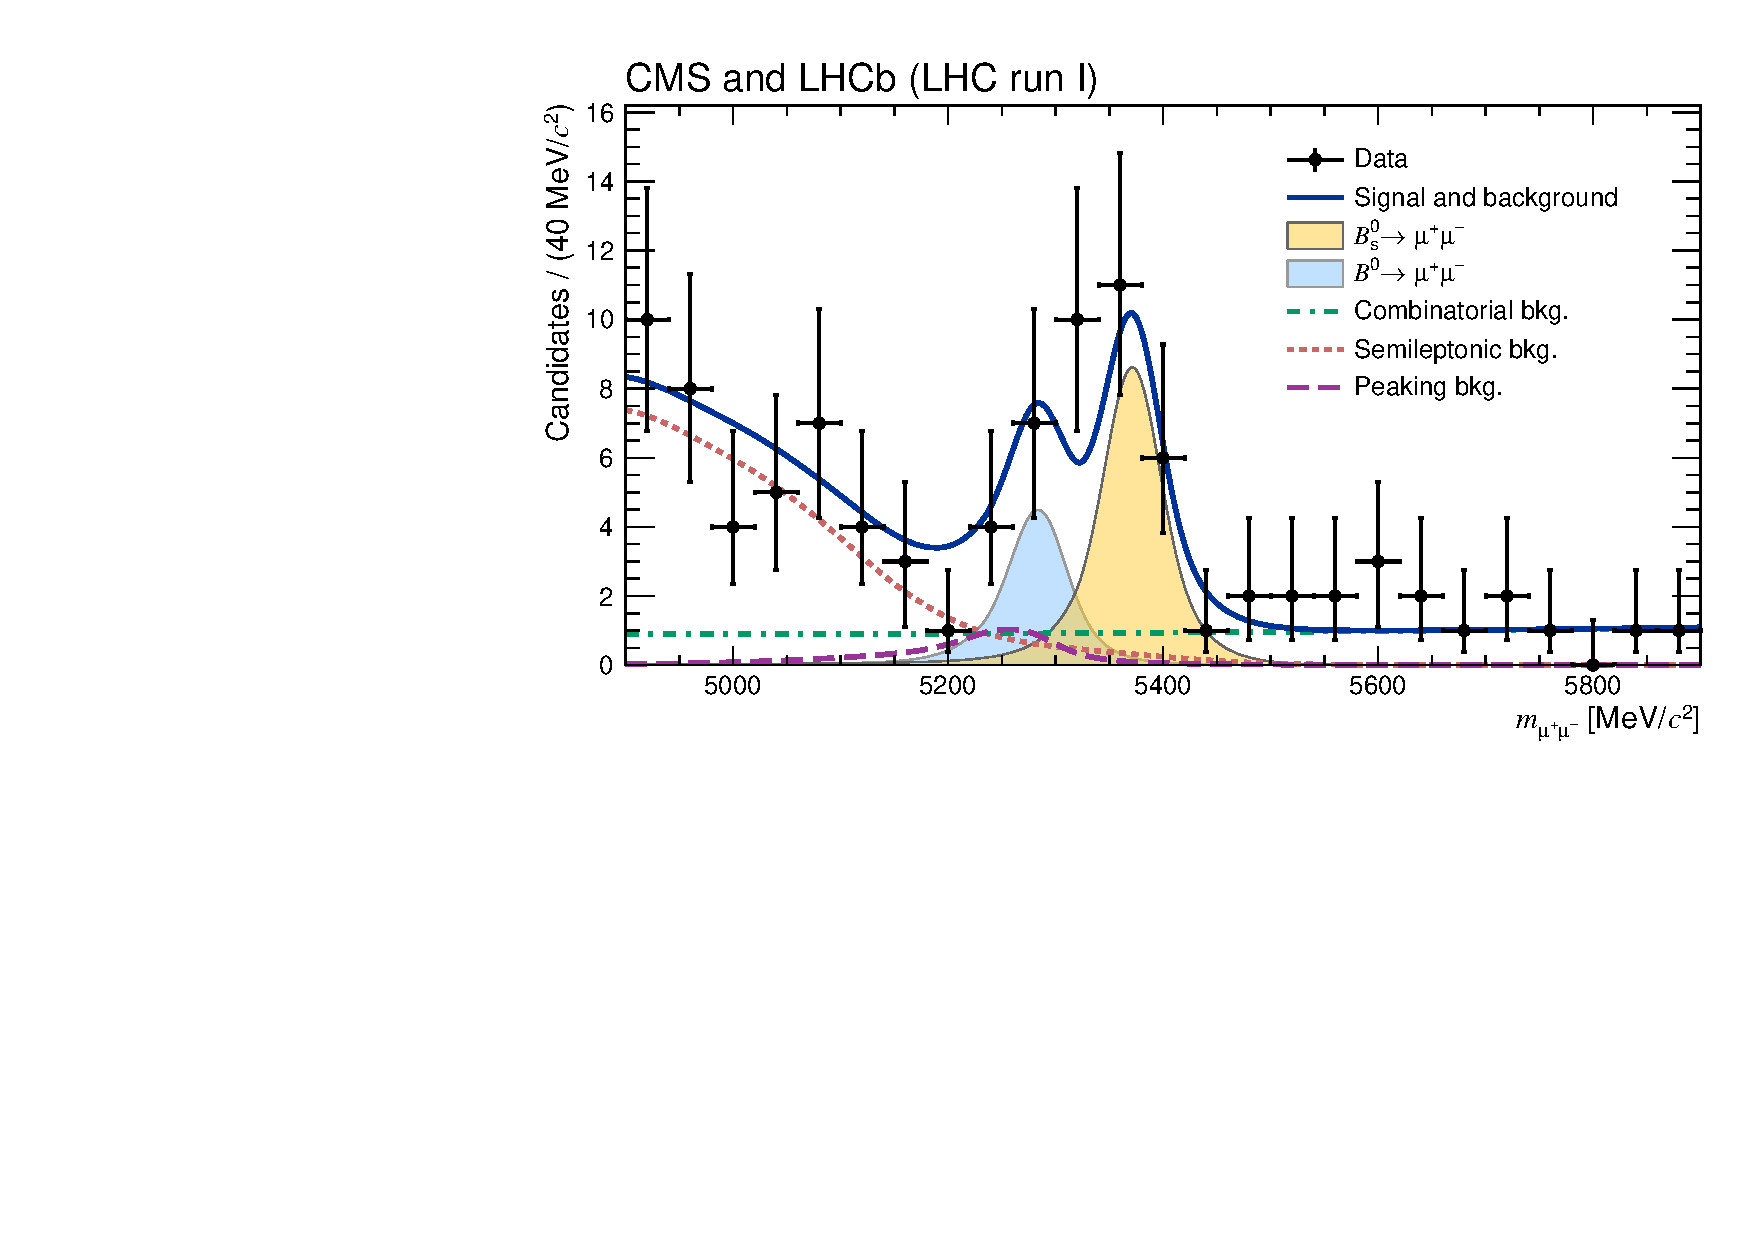
\includegraphics[width=0.6\textwidth]{Introduction/figs/CMSLHCb_EDfig2.pdf}
\caption{Dimuon invariant mass of $B$ candidates showing peaks corresponding 
$\Bs\to\mumu$ and $\Bz\to\mumu$ decays~\cite{CMS:2014xfa}.}
\label{fig:bsmumu}
\end{figure}

\subsection{Semileptonic $\bquark\to\squark\ell^+\ell^-$ decays of \bquark hadrons}
\label{sec:exp_btosll}

At the LHC it is possible to collect large data samples of semileptonic 
decays, especially those with muons in the final state.
Many branching fractions of semileptonic $B$ meson decays were recently measured at
the \lhcb experiment, including $\decay{B}{K\mumu}$, $\decay{B}{\Kstarz\mumu}$
and $\decay{\Bs}{\phi\mumu}$~\cite{LHCB-PAPER-2014-006,LHCB-PAPER-2013-017,LHCB-PAPER-2013-019}. 
Baryon decays were also studied at \lhcb: including 
the rare $\decay{\Lambda_b}{\Lz\mumu}$ decay~\cite{Aaij:2015xza}, whose analysis is described in this thesis.
In contrast to purely leptonic decays, SM predictions for semileptonic decays are affected by the
knowledge of hadronic form factors, which results in relatively large uncertainties,
$\mathcal{O}(30\%)$. As a result measurements are now typically more precise than predictions.

Among the measurements of angular observables that can be affected by 
new physics, particular interest was raised by a set of observables in $\decay{\Bz}{\Kstarz\mumu}$ 
decays, free from factors uncertainties at leading order~\cite{LHCB-PAPER-2013-037}.
Most of the measurements are found to be in agreement with SM predictions
with the exception of the $P'_{5}$ observable, shown in Fig.~\ref{fig:P5prime}, which presents
a local $3.7\sigma$ deviation confirmed by a recent LHCb analysis with higher 
statistics~\cite{Aaij:2015oid} and Belle~\cite{Abdesselam:2016llu}.
Attempts to build a consistent picture point to a new physics contribution
to the Wilson Coefficient $C_9$~\cite{Descotes-Genon:2013wba}.
An angular analysis of $\Bu\to K^+\mumu$ decays was also performed, where observables
are found to be compatible with SM predictions~\cite{LHCB-PAPER-2014-007}.
%
\begin{figure}[h!]
\centering
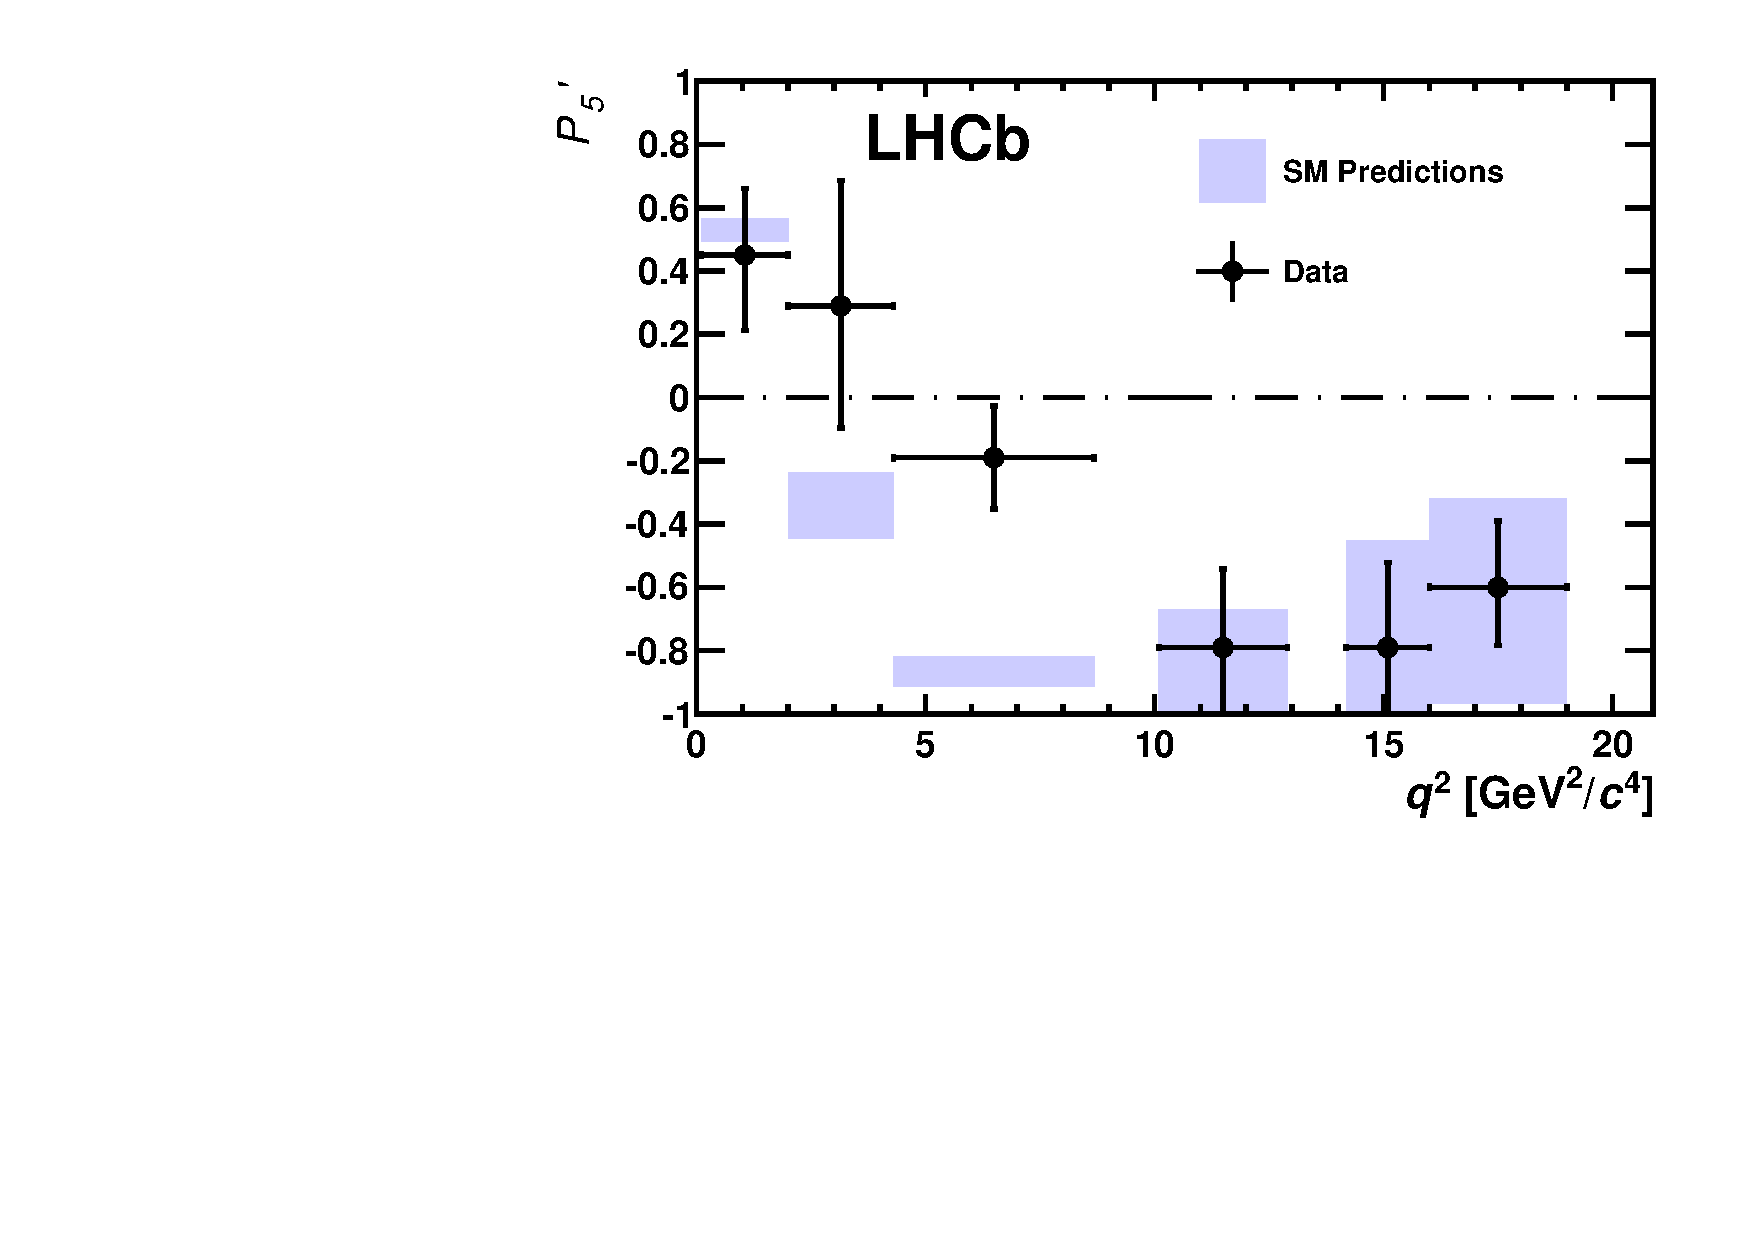
\includegraphics[width=0.6\textwidth]{Introduction/figs/P5prime.pdf}
\caption{Measurement of the $P'_{5}$ observable as a function of \qsq, showing a tension with
SM predictions in the 2--6 \gevgevcccc region~\cite{LHCB-PAPER-2013-037}.}
\label{fig:P5prime}
\end{figure}
%
Other observables for which the sensitivity to form factors effects is reduced are the CP asymmetry between
$B$ and $\bar{B}$ decays, $\mathcal{A}_{CP}$, and the isospin asymmetry between \Bz and \Bu decays, $\mathcal{A}_{CP}$.
Due to the small size of the corresponding CKM elements, CP asymmetries of $\Bz\to K^{(*)}\mumu$
decays are tiny in the SM, $O(10^{-3})$. In BSM models new sources of CP violation can arise and therefore
$\mathcal{A}_{CP}$ measurements are a powerful test of the SM. 
The isospin asymmetry is not zero in the SM due to isospin breaking effects in the form factors.
This is expected to be $\sim1$\% at low \qsq and increase to $\sim10$\% as \qsq tends to zero.
The LHCb experiment, using the full dataset collected in Run I, corresponding to an integrated luminosity of
3~\invfb and $\sim 10^9$ $B$ decays, measured both of these asymmetries to be consistent with
zero~\cite{LHCB-PAPER-2014-006,Aaij:2014bsa}, as reported in Tab.~\ref{tab:AcpAI}. 
%
\begin{table}
\begin{small}
\begin{tabular}{c|cc|cc}
\multirow{2}{*}{}	& \multicolumn{2}{c|}{$\Bz\to K^+\mumu$}			&\multicolumn{2}{c}{$\Bz\to \Kstarz\mumu$}	\\ \cline{2-5}
							& 1.1--6 	[\gevgevcccc]	& 15.0--22.0 [\gevgevcccc] & 	1.1--6 [\gevgevcccc]	& 15.0--19.0 [\gevgevcccc]			\\ \hline
$\mathcal{A}_{CP}$  & $0.004 \pm 0.028$	 				& $-0.005 \pm 0.030$		&	$0.094 \pm 0.047$	& $-0.074 \pm 0.044$ 	\\
$\mathcal{A}_{I}$	& $-0.10^{+0.08}_{-0.09} \pm 0.02$	& $-0.09 \pm 0.08 \pm 0.02$	&	$0.00^{+0.12}_{-0.10} \pm 0.02$  &	$0.06^{+0.10}_{-0.09} \pm 0.02$ \\
\end{tabular}
\end{small}
\caption{Measurement of CP and isospin asymmetry in $\Bz\to \Kstarz\mumu$ decays from the LHCb experiment~\cite{TomRDreview}.  }
\label{tab:AcpAI}
\end{table}
%
Recently, progress was also made measuring electron channels.
The branching fraction of the $\Bz\to\Kstarz\ee$ decay was measured to be $(3.1\pm1.3)\times10^{-7}$ in the dilepton mass interval 30--1000~\mevcc~\cite{LHCB-PAPER-2013-005}. Furthermore, for the first time
angular observables were measured for this decay and found to be consistent with SM predictions~\cite{Aaij:1981106}.

Given the wide set of available measurements, theorists have implemented global fits including results from rare decays analyses,
 as well as inputs from \Bs mixing and Higgs measurements, in order to understand if the existing anomalies could be caused by a common factor.
The results of such global fits agree that there is a tension with respect to the SM at the level of 3--4 standard deviations,
depending on the set of assumptions made. In particular they favour a shift $C^{NP} \sim -1$ to the $C_9$ Wilson
Coefficient, related with the penguin diagram mediated by a $Z^0$ boson~\cite{Altmannshofer:2014rta,Descotes-Genon:2013wba,Hurth:2016fbr}. 

\subsection{Lepton Flavour Violation searches}

Several Lepton Flavour Violation (LFV) searches are linked to rare decays as they involve small branching
ratios in the SM that can be enhanced by BSM physics. %They are therefore a natural place to look for new physics.
Lepton flavour conservation is experimentally well-established measuring the branching ratios of
decays of muons into electrons and no neutrinos, but has no strong theoretical
explanation in the context of the SM. In fact it is already observed that flavour
is not conserved in neutrino oscillations. 
%This section reports a short review of LFV searches. 
%
The best-studied decays violating lepton flavour 
are rare muon decays including $\mu^+\to e^+\gamma$ and $\mu^+\to e^+e^-e^+$.
Since muons can be abundantly produced and the final states are simple,
these decays provide the best constraints to LFV. The current best upper limits are $1.2 \times 10^{-11}$
for the radiative decay and $1.0 \times 10^{-12}$ for \mbox{$\mu^+\to e^+e^-e^+$} obtained
respectively by the MEGA~\cite{Ahmed:2001eh} and SINDRUM~\cite{Bellgardt:1987du} experiments.
Several LFV searches in the $B$ sector have recently been performed at the LHCb experiment 
including decays such as $\Bz\to e\mu$~\cite{LHCB-PAPER-2013-030} and $\tau$ decays such
as $\tau\to\mumu\mu$~\cite{LHCB-PAPER-2013-014}. None of these searches has found evidence 
of new physics so far and therefore they set limits, constraining the parameter space available for BSM models.
Figure~\ref{fig:LFV_decay} shows a summary of the best limits set at different times
on LFV searches~\cite{Marciano:2008zz}.


\begin{figure}[h!]
\centering 
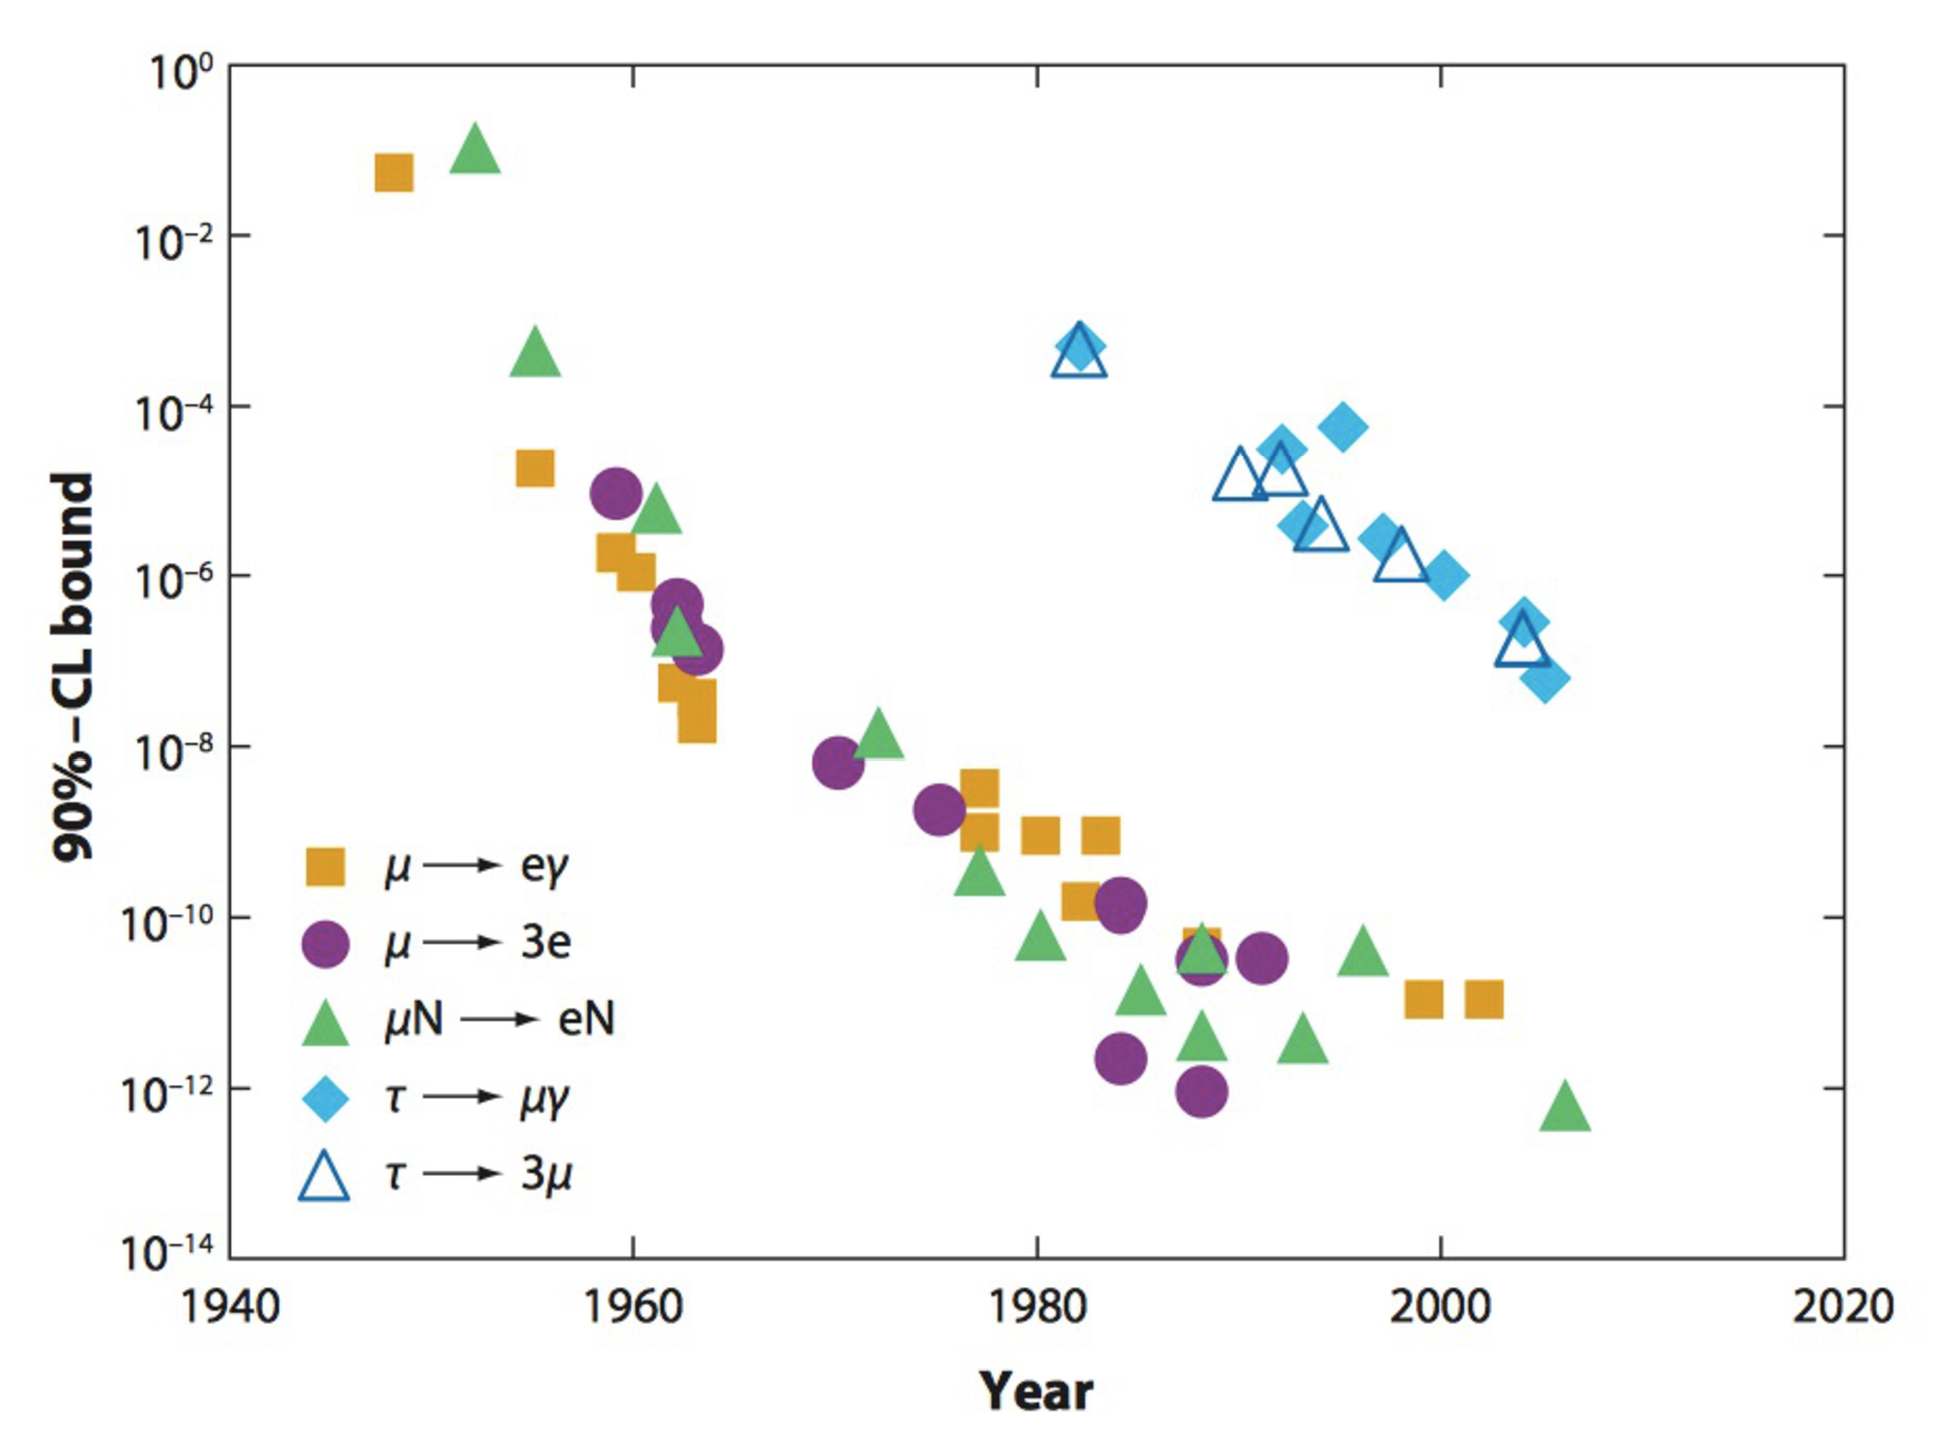
\includegraphics[width=0.7\textwidth]{Introduction/figs/LFV.pdf}
\caption{Summary of limits set in LFV searches as a function of time~\cite{Marciano:2008zz}.}
\label{fig:LFV_decay}
\end{figure}
 


\subsection{Monte Carlo corrections}

Since the MC samples available show some discrepancies with data we apply weights to lower these discrepancies.
Weighted MC is used thoughout all the process: to get shapes for the fit, to get efficiencies, to train the Neural Networs.
In the following section are described the contribution considered.

\subsubsection{\Bz transverse momentum and number of SPD hits}

First of all, we reweight our MC to match data distributions of \Bz transverse momentum.
To do this we need to compare the \Bz $p_T$ distributions in data and MC.
This cannot be done trivially because the real data events contain background.
Therefore we vfit $\Bz\to\Kstar(\jpsi\to ll)$ events out of stripping and we use it to extract an S-weight.
The S-weight, corresponds to the probability of each event to be signal given its mass.
The fits used to extract the S-weight are reported in Fig.\ref{fig:SweightFit} 

Now combining the real data distribution and the S-weight we obtaine a "clean signal" transverse momentum
distribution which can be compared to the same distribution in MC. We take the ratio of the two
distributions as a weight for the MC. This brings the MC distribution to match the real data one by construction.
The described procedure is done separately for 2011 and 2012 events, for muons and electrons.
In Fig.\ref{fig:B0ptW} is reported the weight in isoposulated bins of \Bz $p_T$ for the electrons and muons channel, for 2011 and 2012 data. 

One other quantity that the MC is known to underestimate is the number of SPD hits important especially
for electron identification. We apply in this case the same procedure used for the \Bz transverse momentum.
In Fig.\ref{fig:SPDW} is reported the weight in isoposulated bins of number of SPD hits for the electrons and muons channels, for 2011 and 2012 data.


\begin{figure}[h!]
\centering
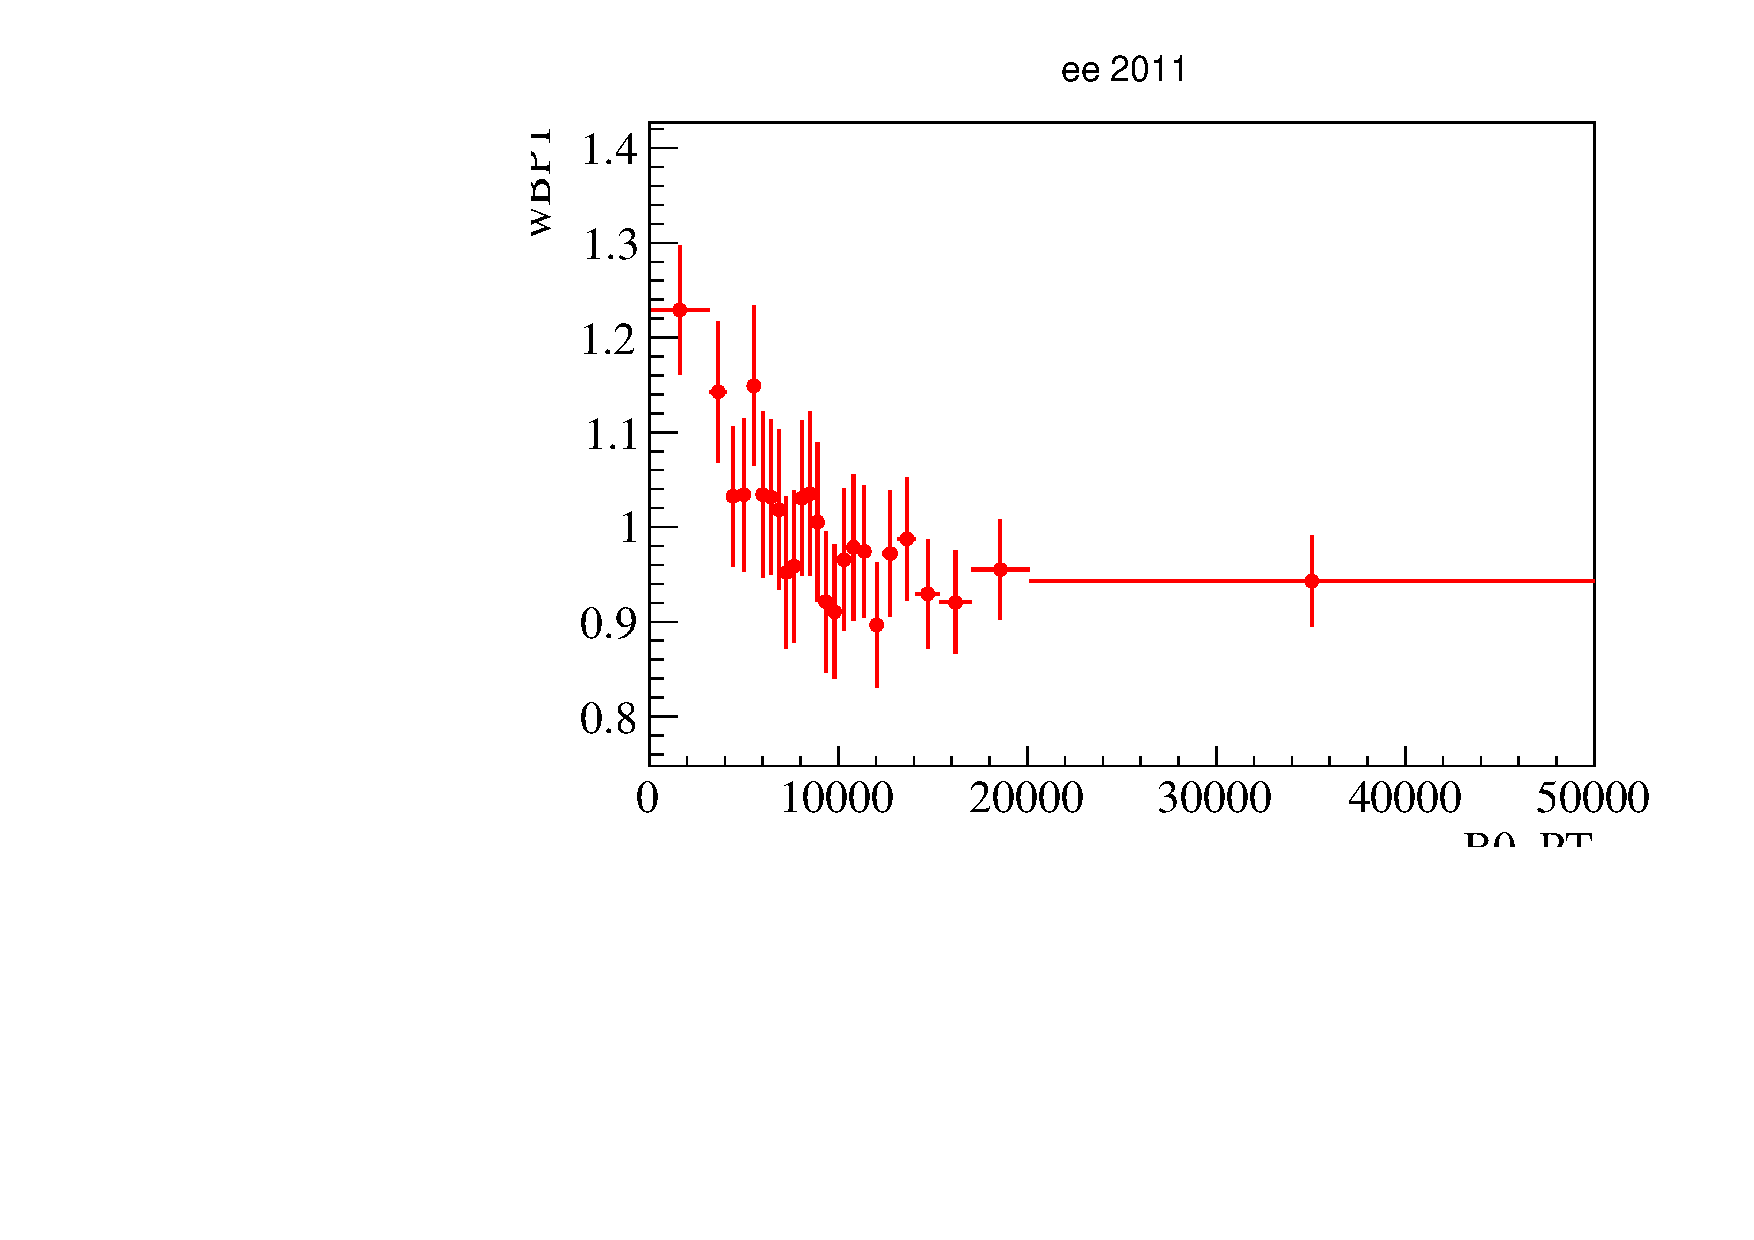
\includegraphics[width=0.40\textwidth]{RKst/figs/Weights/EE_wBPT_2011.pdf}
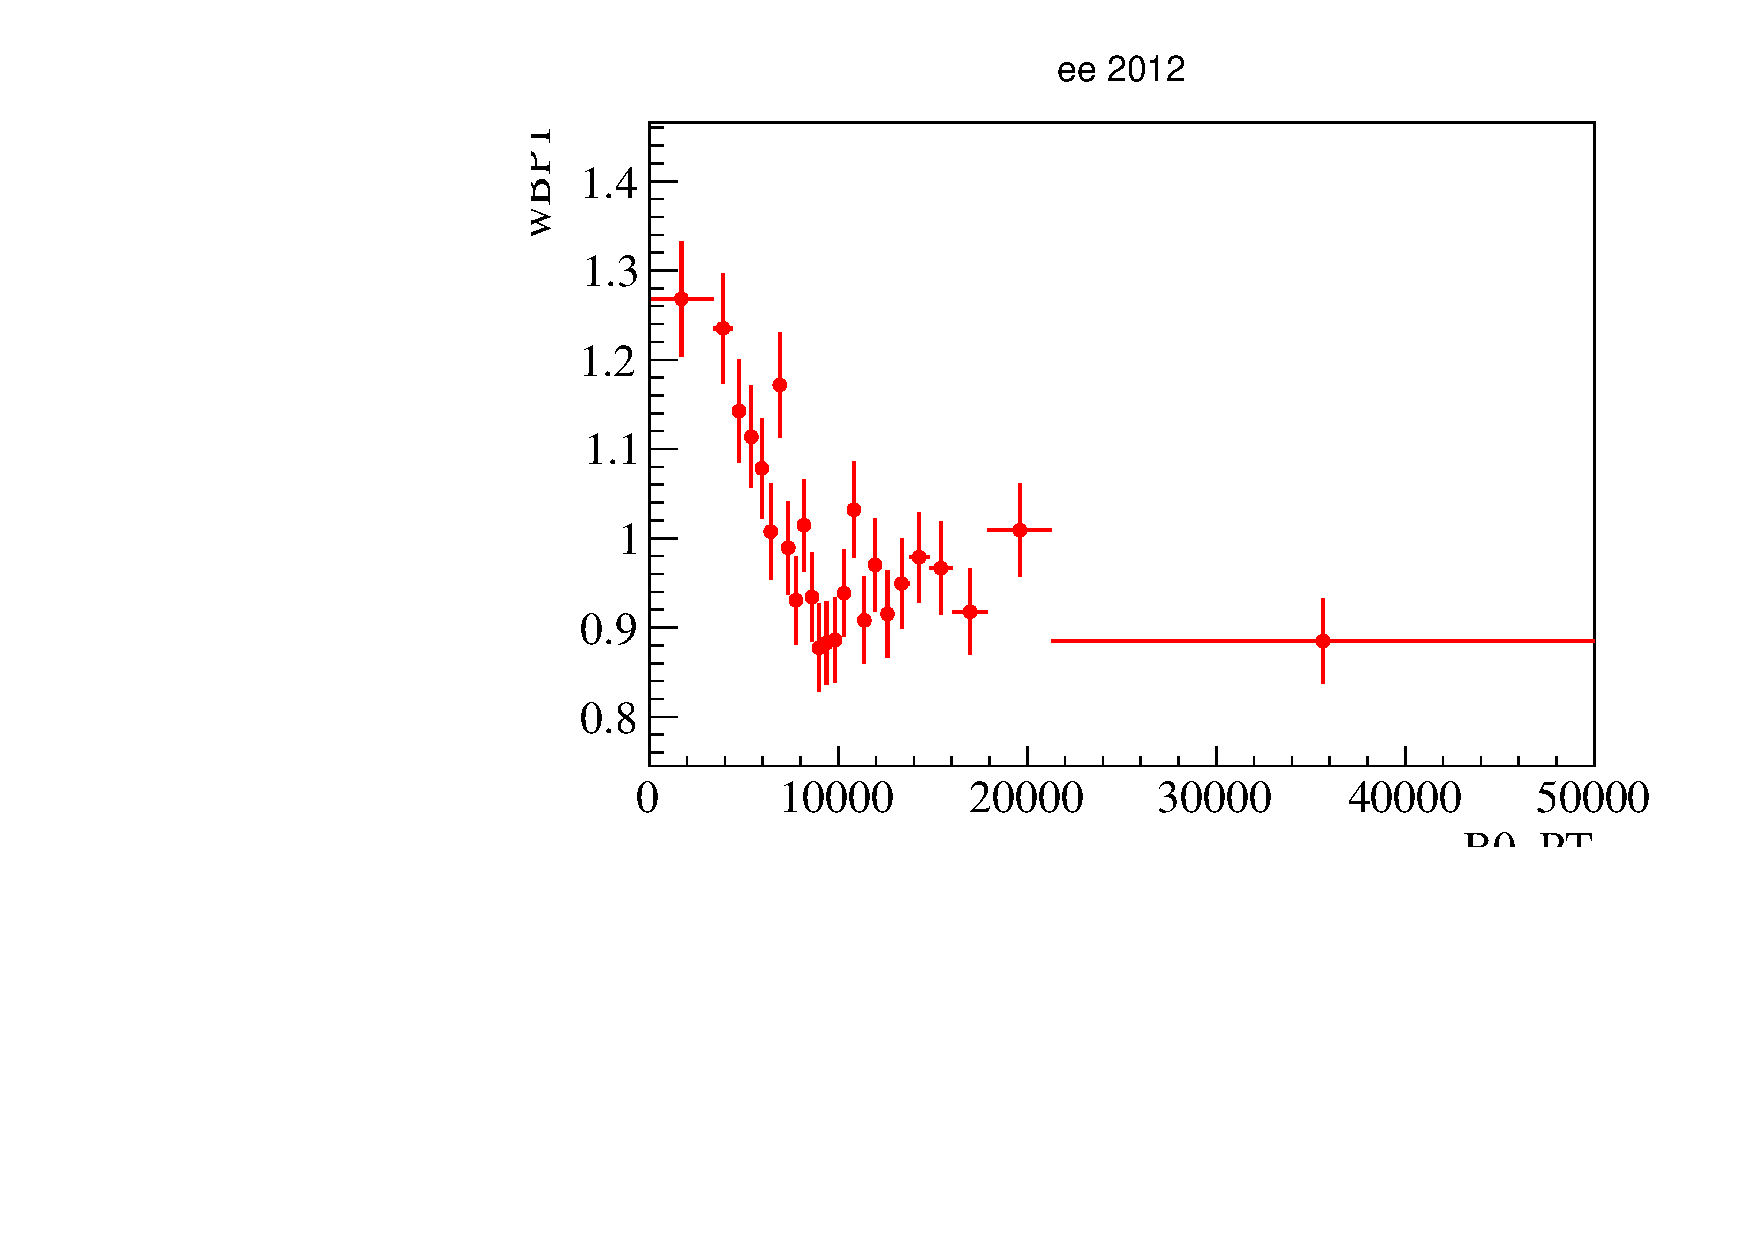
\includegraphics[width=0.40\textwidth]{RKst/figs/Weights/EE_wBPT_2012.pdf} \\
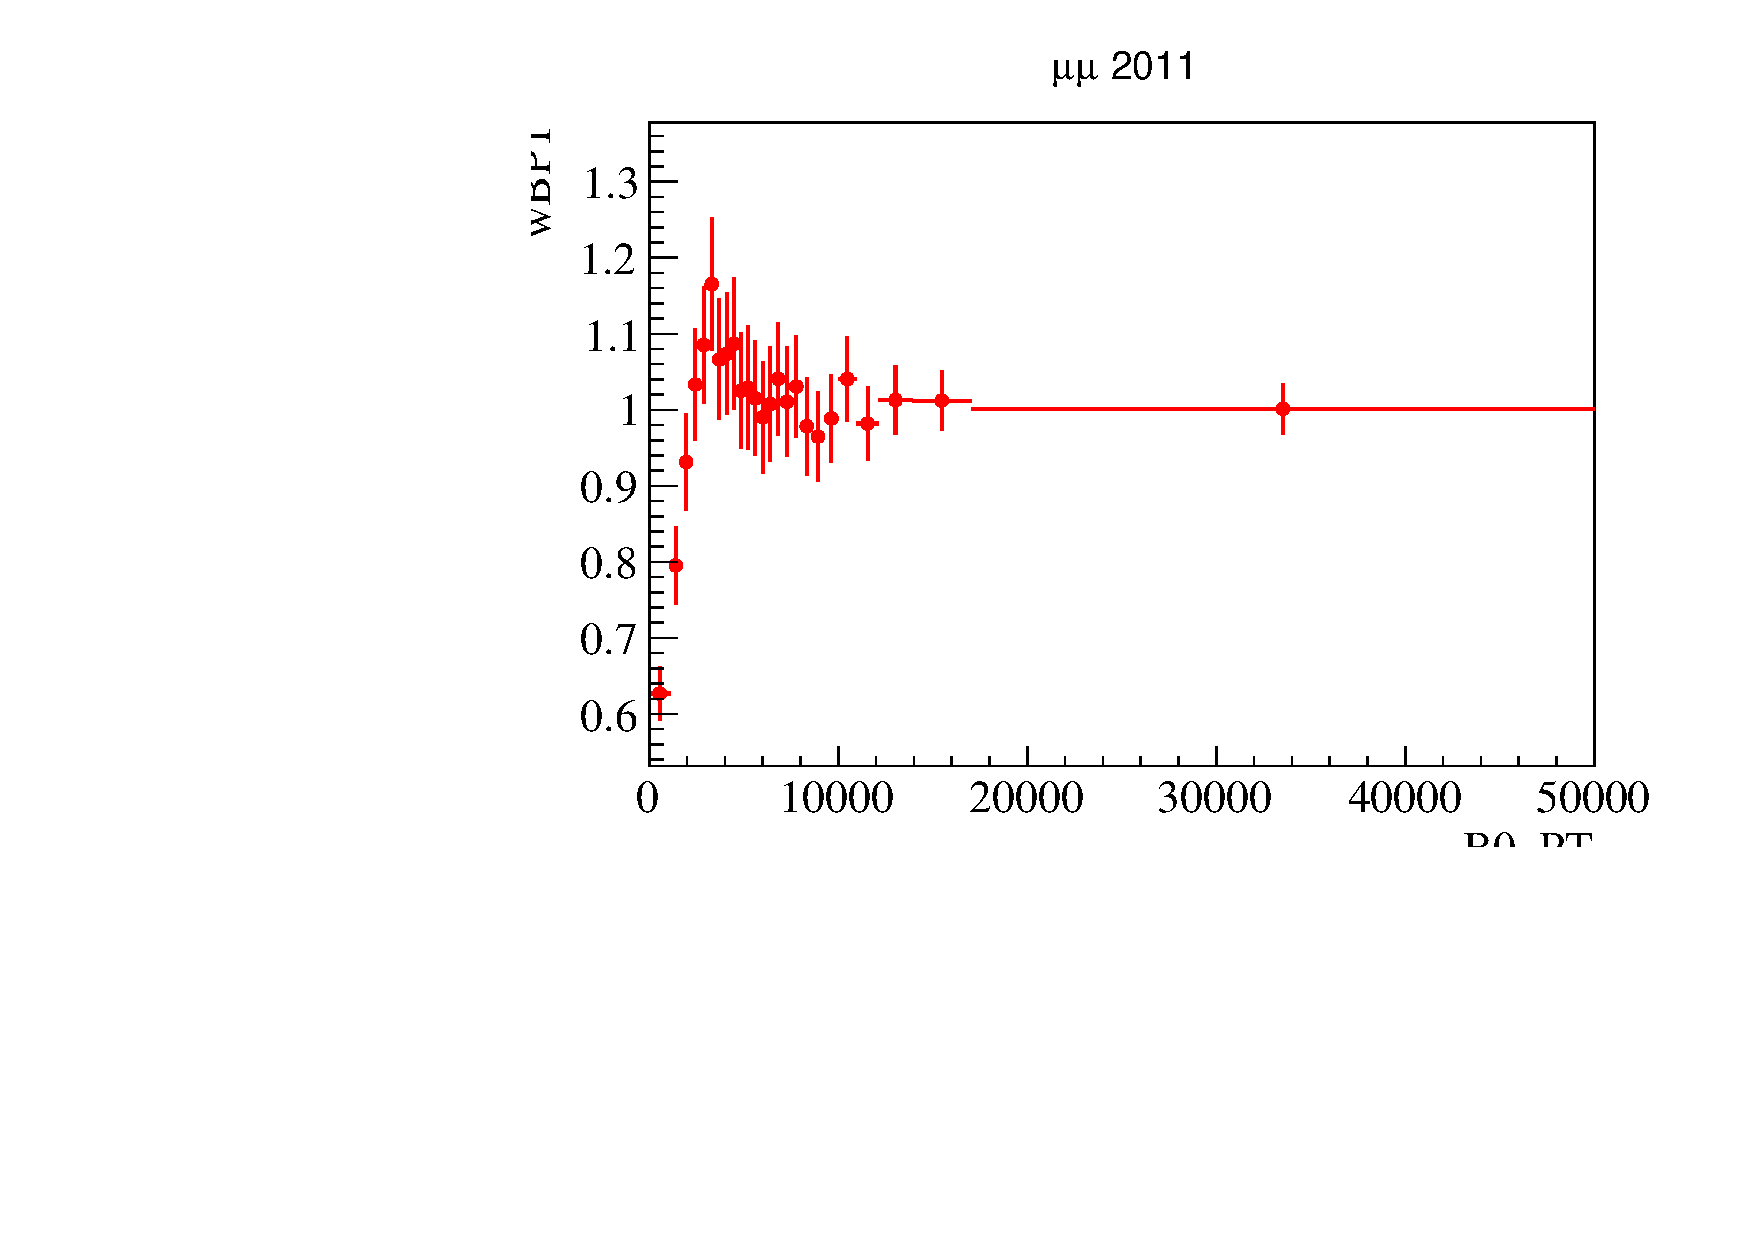
\includegraphics[width=0.40\textwidth]{RKst/figs/Weights/MM_wBPT_2011.pdf}
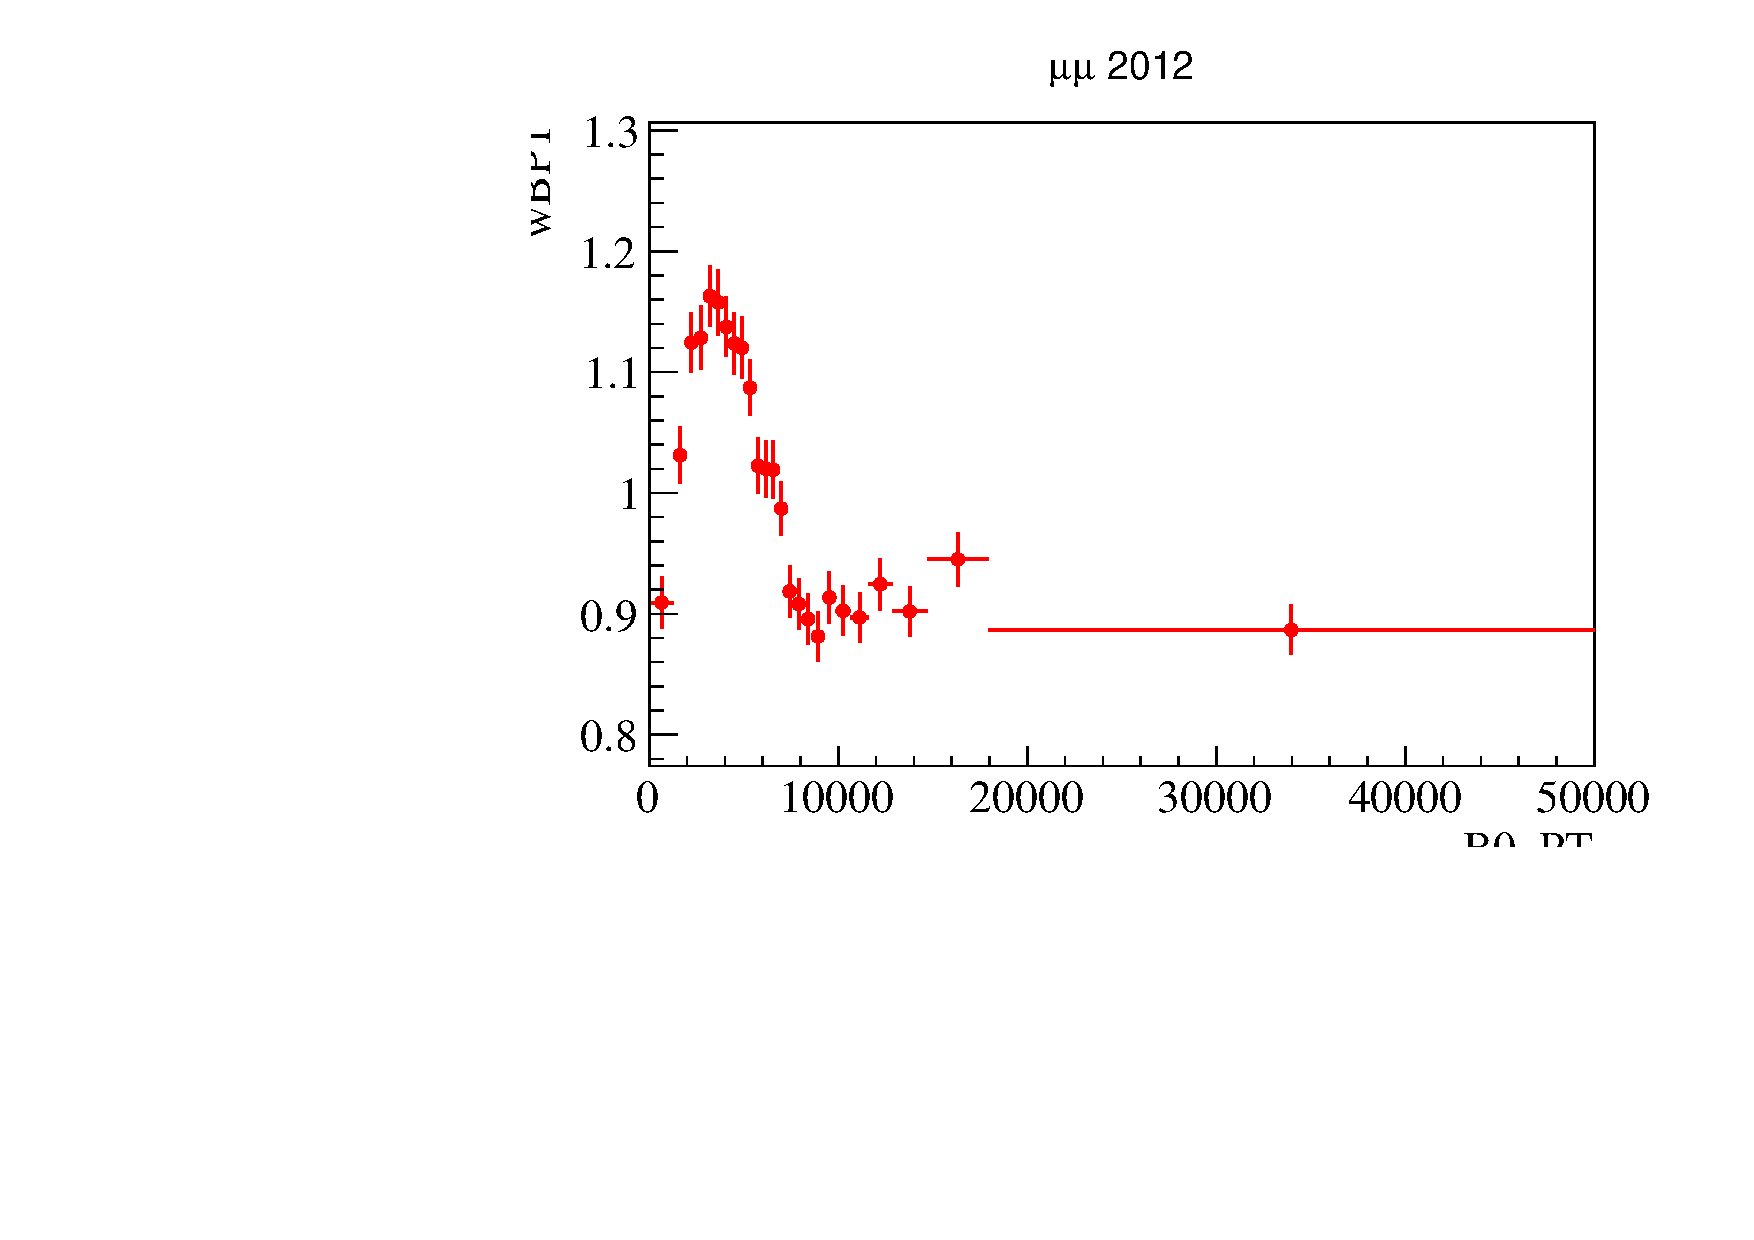
\includegraphics[width=0.40\textwidth]{RKst/figs/Weights/MM_wBPT_2012.pdf}
\caption{Weight applied to MC events in isoposulated bins of \Bz $p_T$ for the electrons (top) and muons (bottom) channel, for 2011 (left) and 2012 (right) data. }
\label{fig:B0ptW}
\end{figure}

\begin{figure}[h!]
\centering
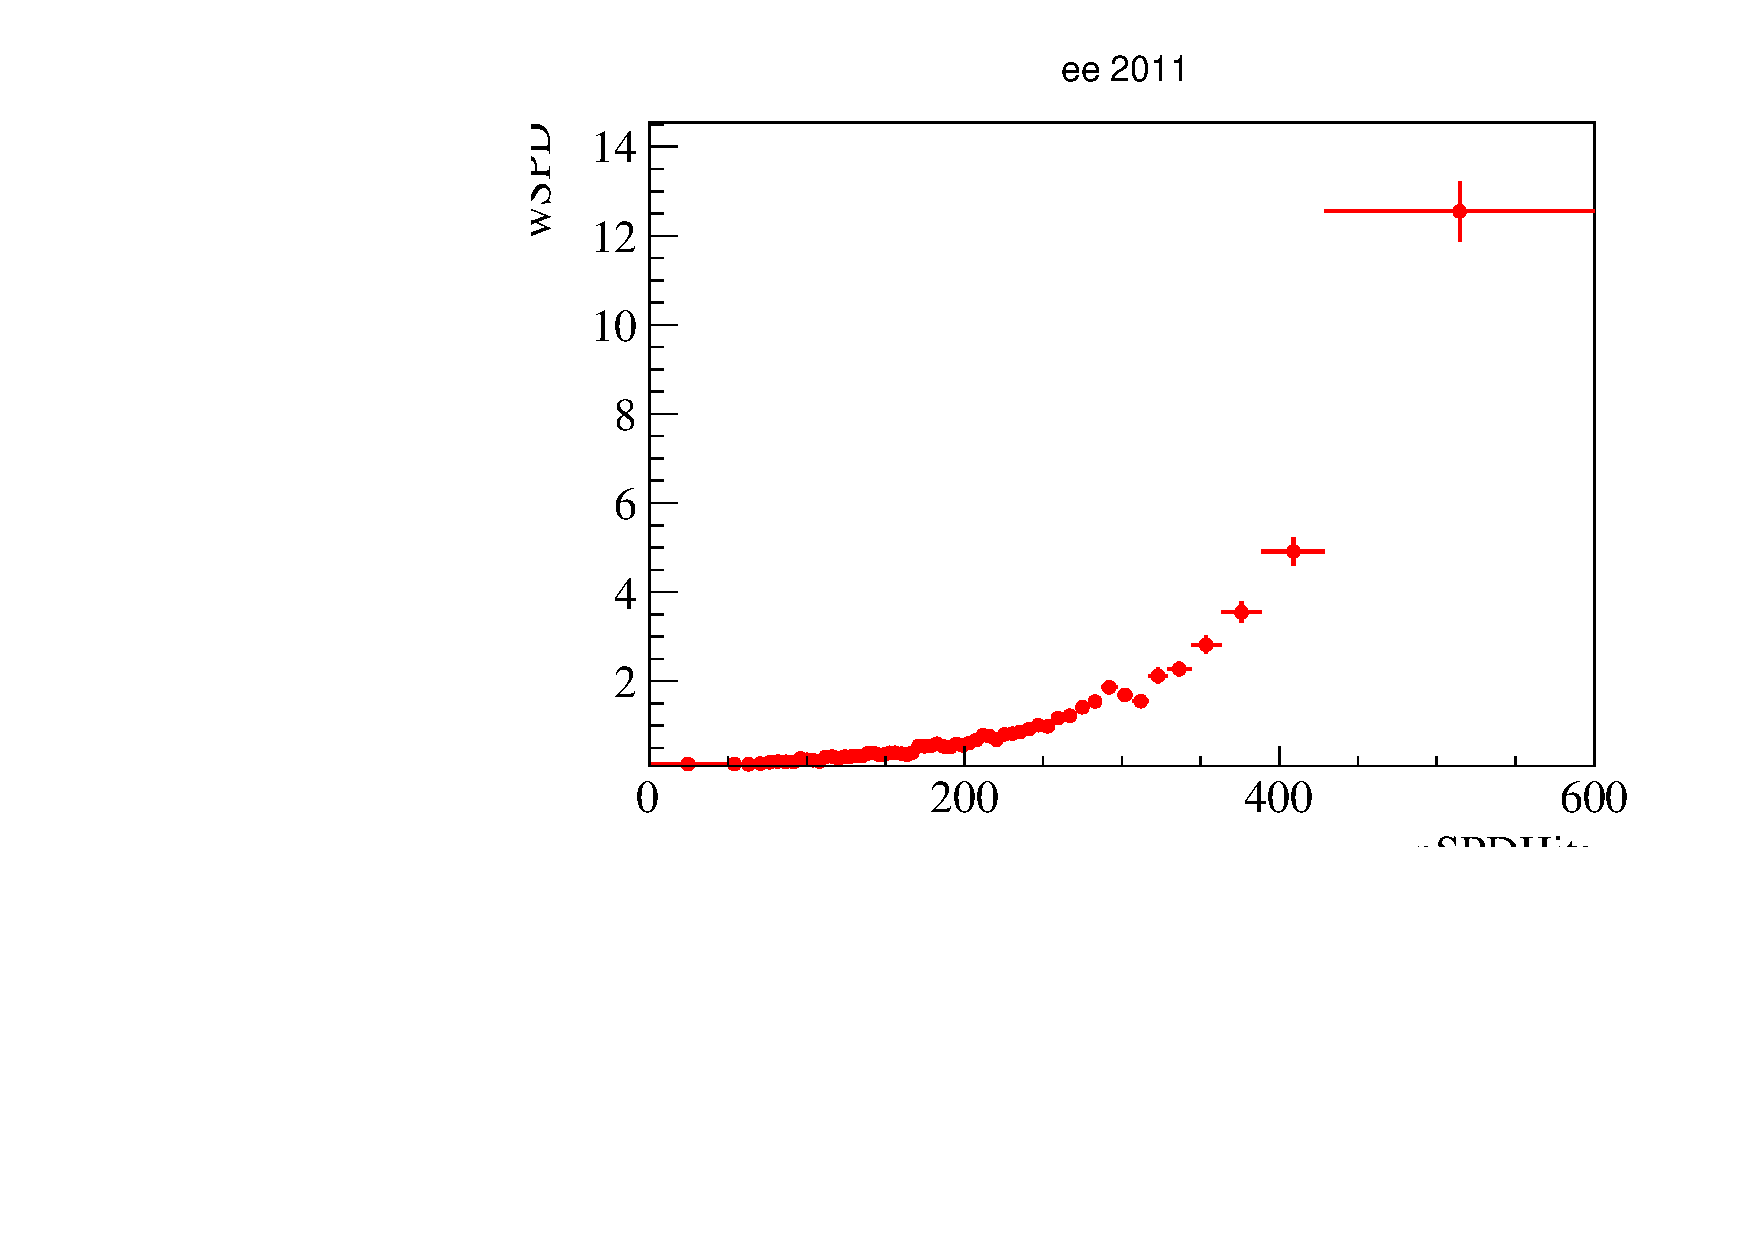
\includegraphics[width=0.40\textwidth]{RKst/figs/Weights/EE_wSPD_2011.pdf}
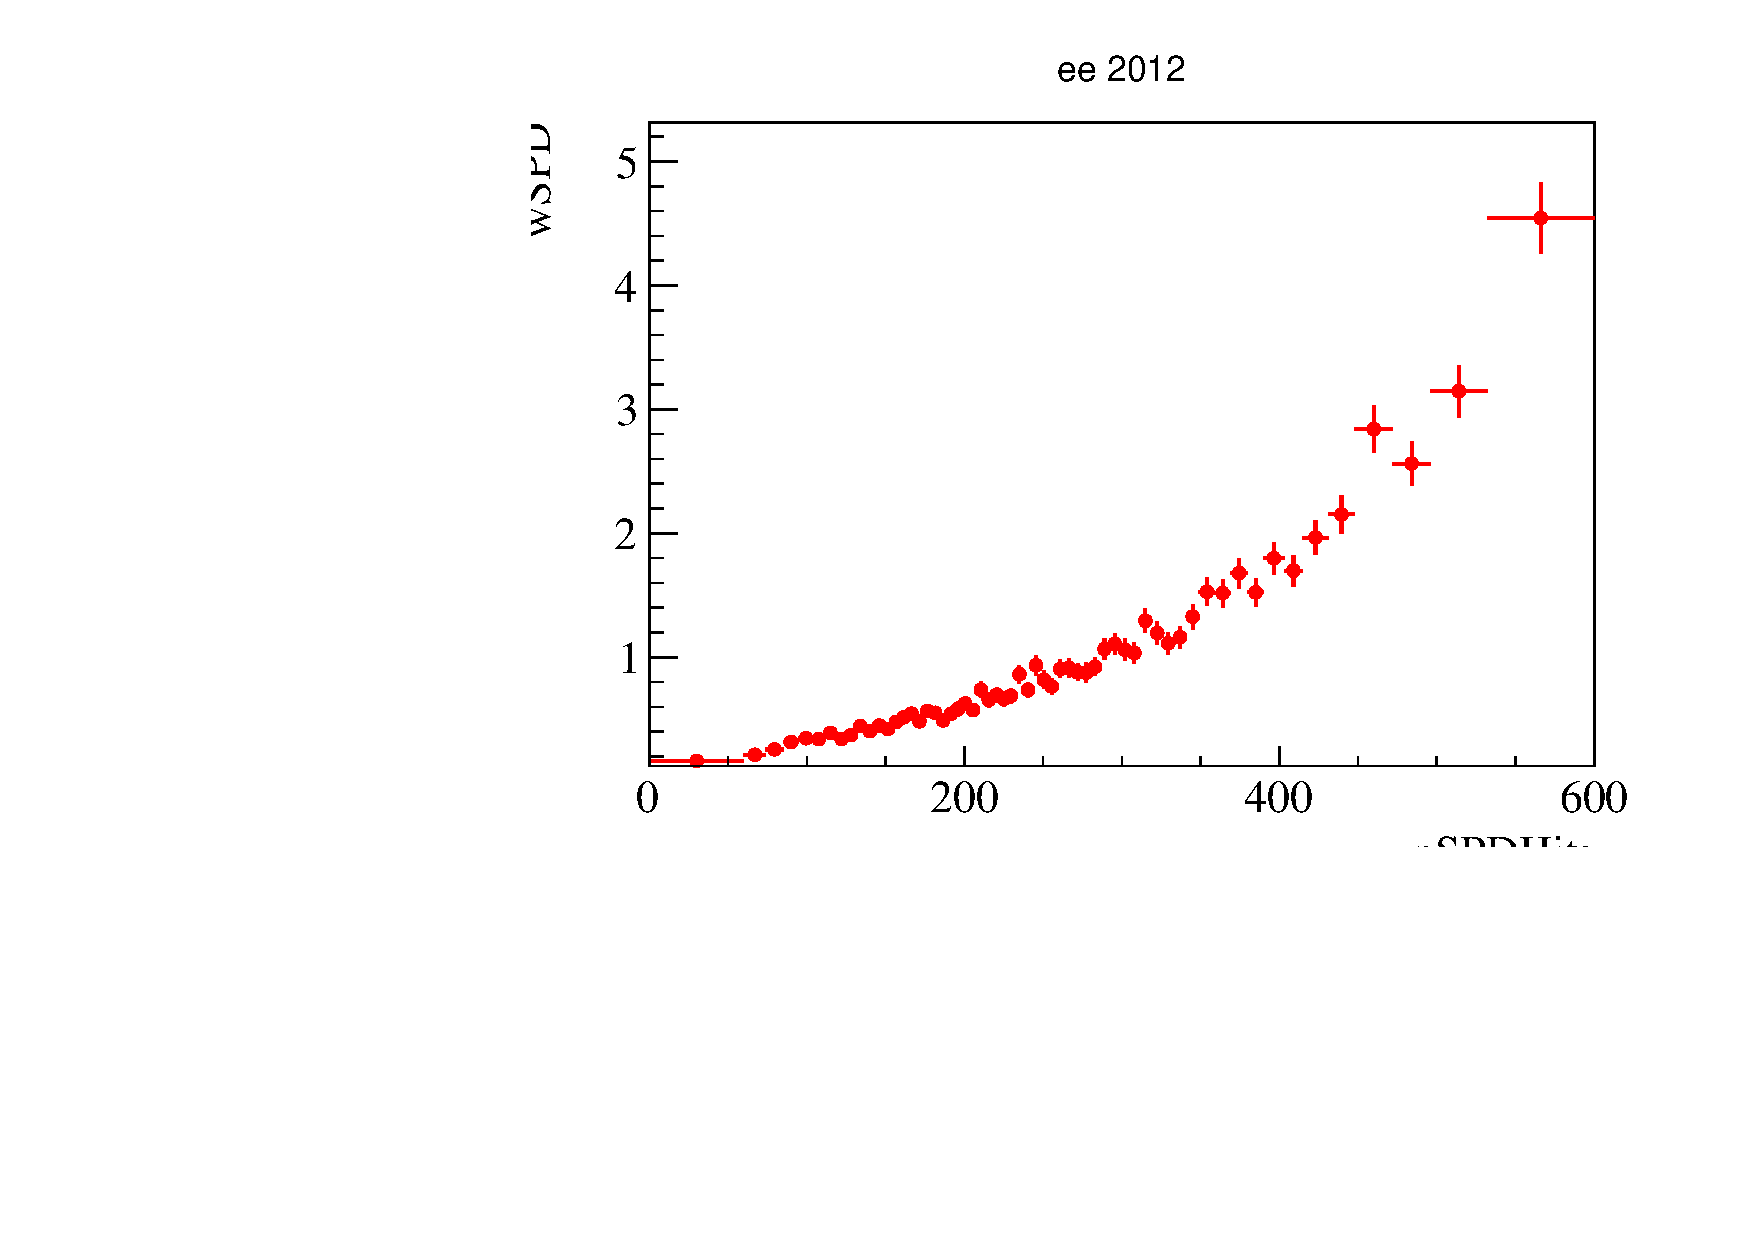
\includegraphics[width=0.40\textwidth]{RKst/figs/Weights/EE_wSPD_2012.pdf} \\
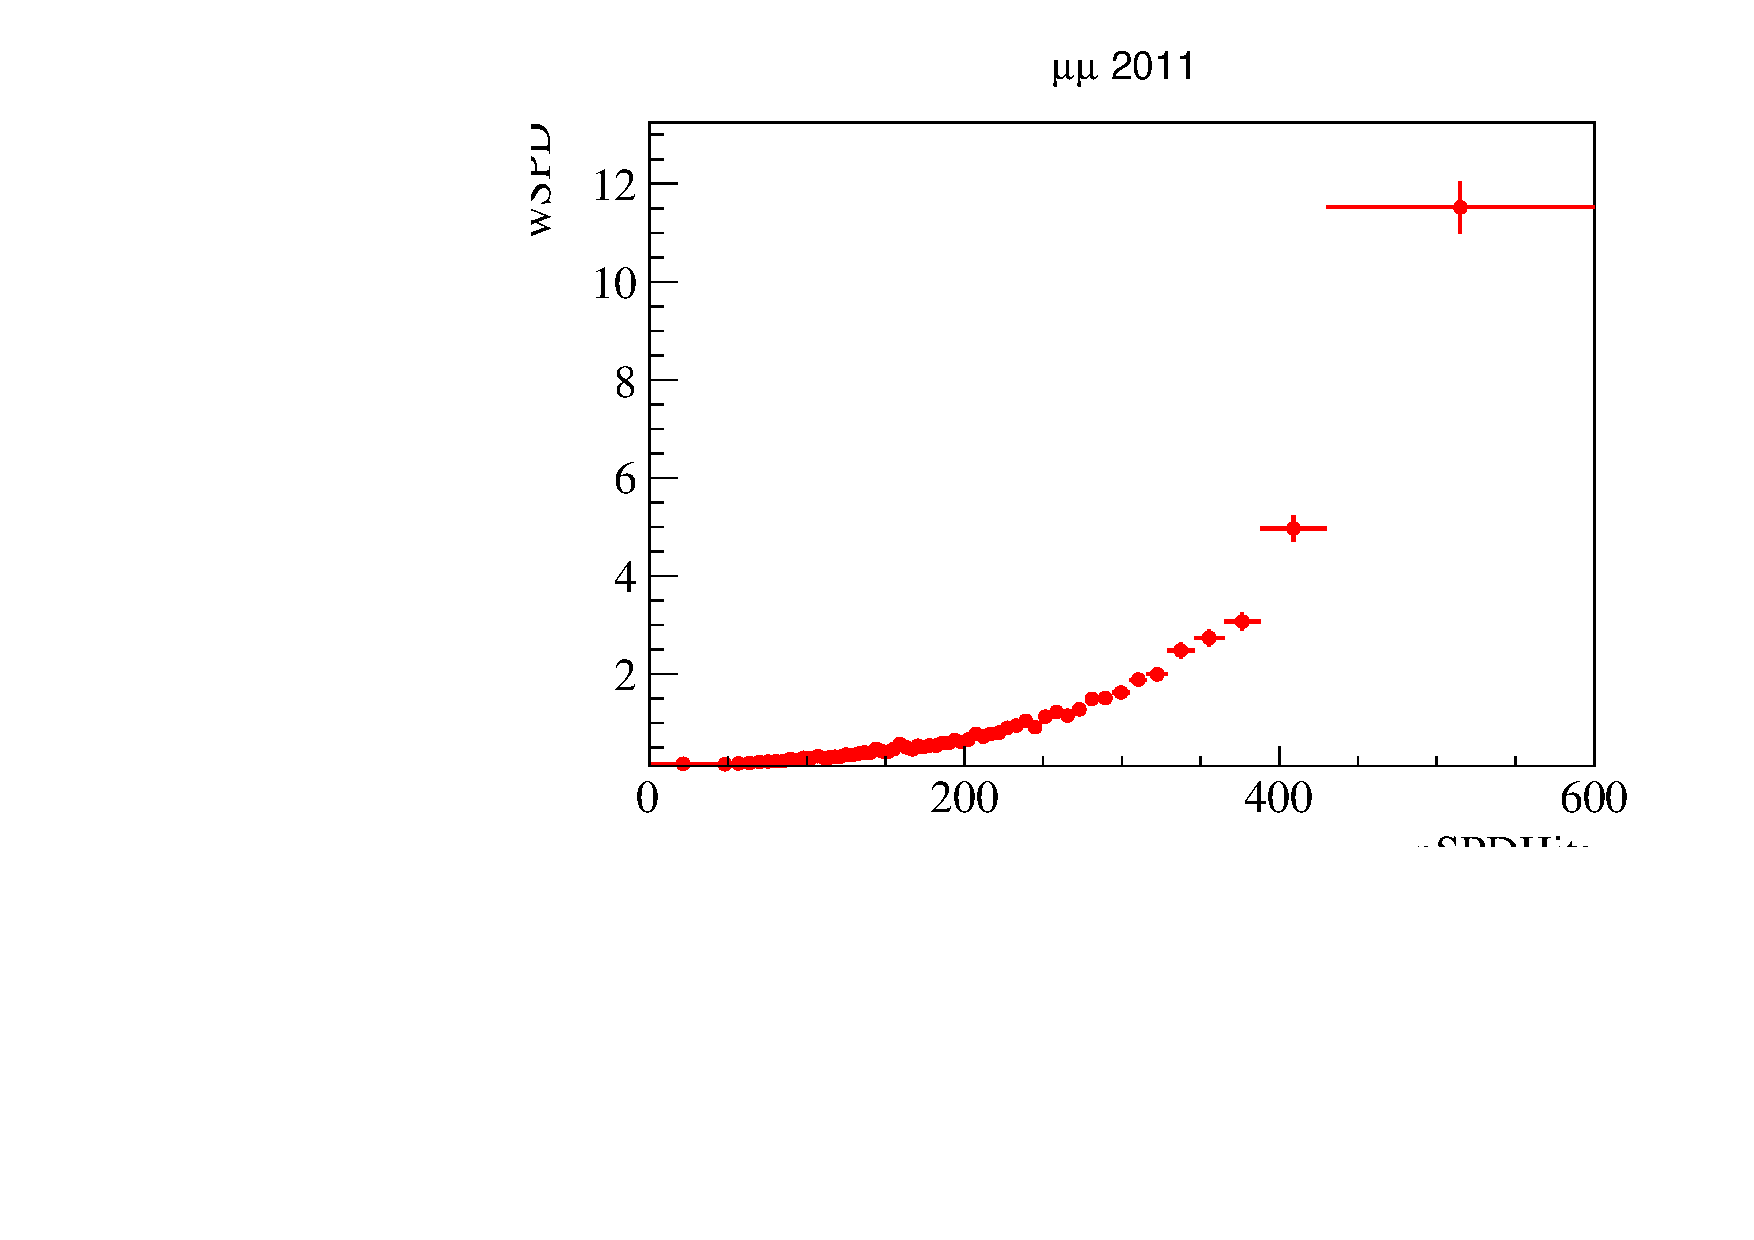
\includegraphics[width=0.40\textwidth]{RKst/figs/Weights/MM_wSPD_2011.pdf}
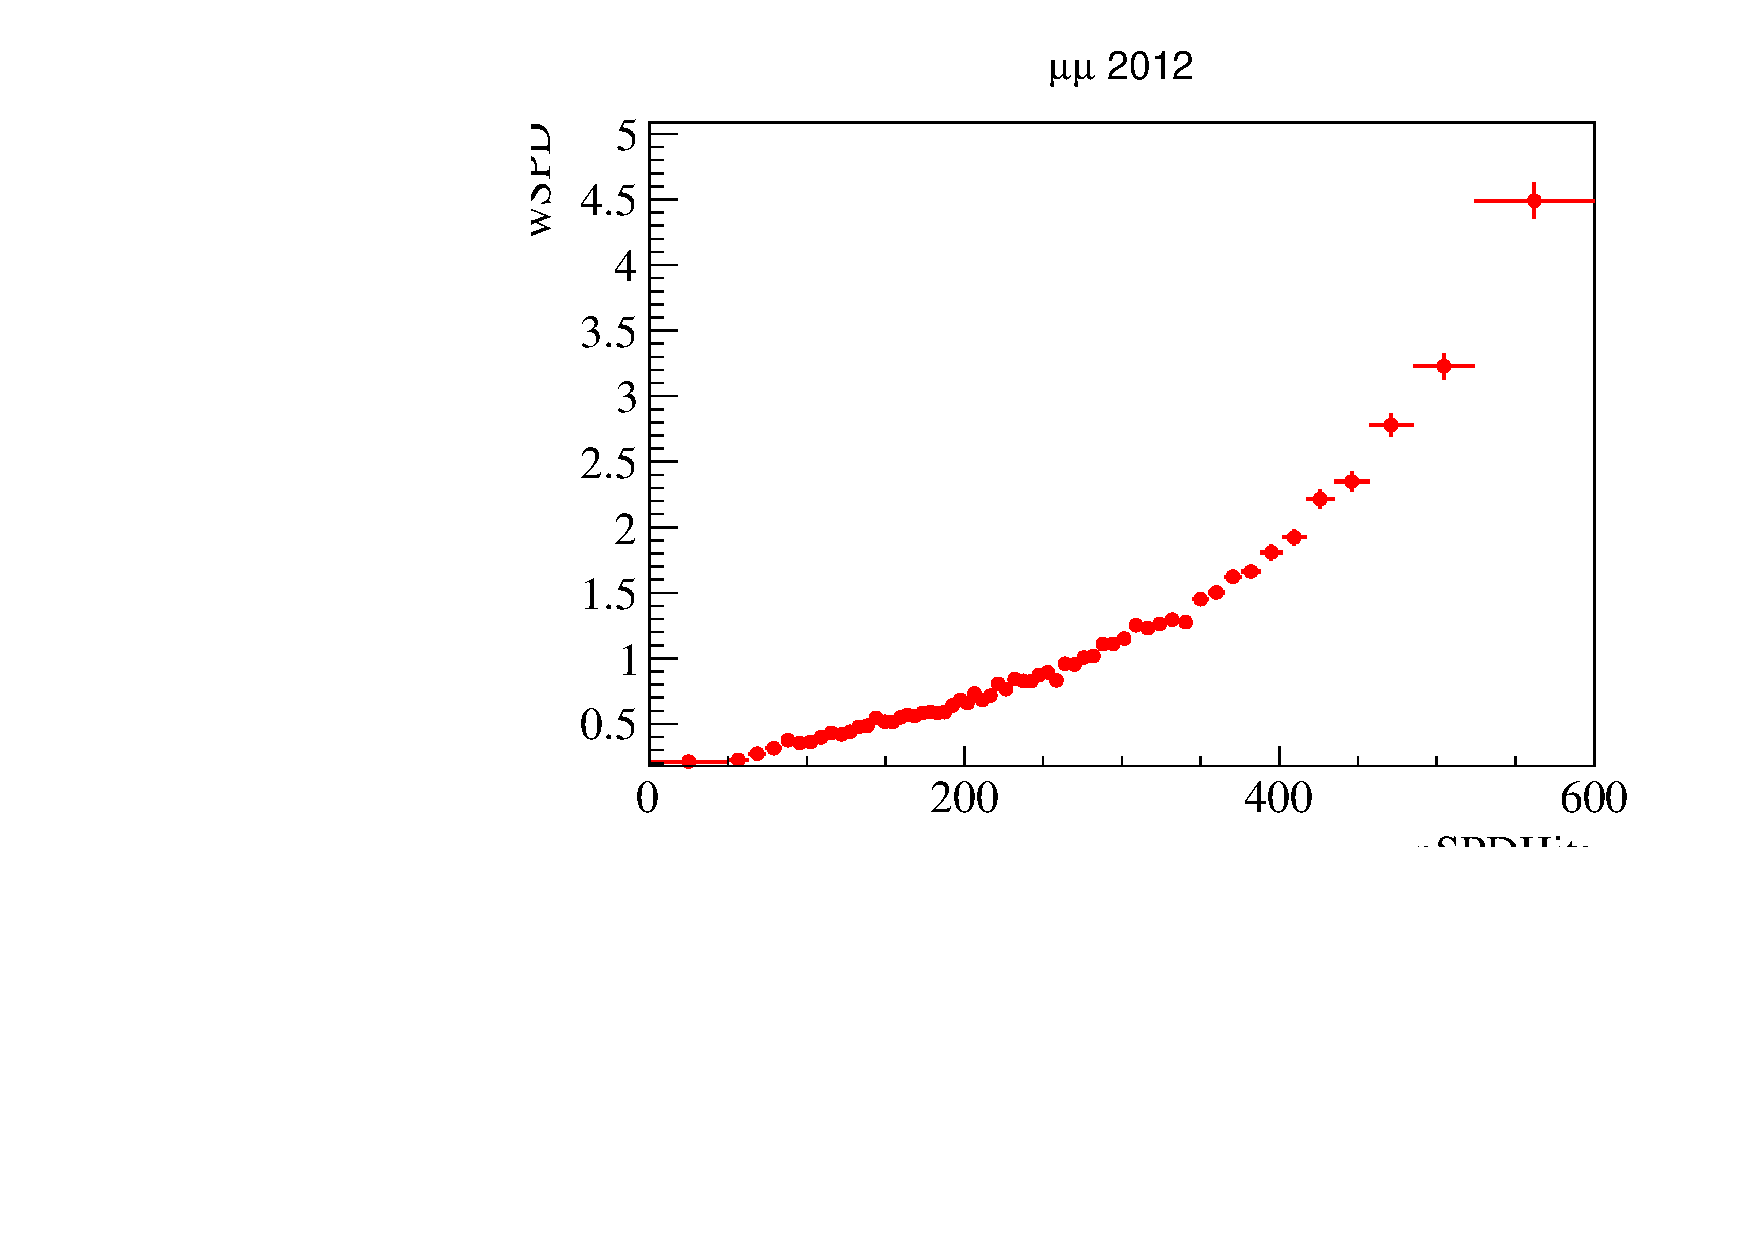
\includegraphics[width=0.40\textwidth]{RKst/figs/Weights/MM_wSPD_2012.pdf}
\caption{Weight applied to MC events in isoposulated bins of number of SPD hits for the electrons (top) and muons (bottom) channel, for 2011 (left) and 2012 (right) data. }
\label{fig:SPDW}
\end{figure}

\subsubsection{PID weighting}

The PID variables are also known not to match between data and MC. For this reason we use a data drive method to find the efficiency as
descibed in \ref{sec:PIDeff}. Nevertheless the MC is used to find shapes to use in the fits and these shapes could be affected
by the differences in the PID variables. For this reason we use the same data driven method to get a table of PID efficiencies
as a function of momentum and pseudorapidity of tracks and we use this to reweight out MC. More details can me found in \ref{sec:PIDeff}.

\subsubsection{Trigger efficiency}

{\em Simone scrivi qualcosa io di sta roba non so nulla}



\clearpage



\section{Selection}
\label{sec:RKst_selection}

The selection process, described in this section, is divided into several steps:
\begin{itemize}
\item candidates have to fall into the detector acceptance, produce hits and be selected
on the basis of quality variables, such as \chisq of tracks and vertices and basic kinematic cuts.
%This stage is called ``stripping". 
Furthermore, it is required that the events are triggered by specific
trigger lines and cuts are applied to remove backgrounds from specific decays.
All these first three steps are referred to as ``pre-selection";
\item secondly, PID requirements are applied to remove part of misreconstructed
background and clear the way for the last step;
\item in the final step a neural network is used to remove combinatorial background. Furthermore,
for the electron channels, which are more challenging, the kinematic structure of the decays
is also used to improve the purity of the samples.
\end{itemize}
%
%In order to minimise the systematic uncertainties the same selection requirements are used to select 
%the rare signal candidates and the relative charmonium channel, a part from the \qsq cuts which serve
%to distinguish them. 
To identify the $\jpsi(\mu\mu)$ candidates a dimuon invariant mass
interval of 100~\mevcc~around the nominal \jpsi peak~\cite{PDG2014} is selected.
On the other hand, it is not possible to use a narrow interval around $\jpsi(ee)$ mass peak as the invariant mass
distribution is characterised by a long radiative tail at low masses due to bremsstrahlung radiation.
Furthermore, a requirement on $m(ee)$ would distort the 4-body $m(K\pi ee)$ mass distribution. This is not advisable 
as it is important to be able to fit a wide mass range to constrain the backgrounds. For these reasons the interval used to 
select $\jpsi(ee)$ candidates extends as low as possible in \qsq without overlapping with
the rare channel interval. Candidates are therefore identified as $\jpsi(ee)$ if they fall in the \qsq interval
$6 < \qsq < 11$~\gevgevcccc. Similarly, candidates are identified as $\psitwos(ee)$ is they fall into $11 < \qsq < 15$~\gevgevcccc
and $\gamma(ee)$ if they fall into $\qsq < 0.0004$~\gevgevcccc.
Table~\ref{tab:candidates} summarises the requirements used to distinguish samples corresponding to different decay channels.
Figure~\ref{fig:2D_q2_B0mass} shows two-dimensional distributions of \qsq versus the 4-body invariant mass 
for candidates passing the full selection. Horizontal bands can be clearly seen at \qsq values corresponding to the \jpsi and \psitwos resonances.
On the plot for muons a vertical band which corresponds to the rare decay is also evident.

\begin{table}[t!]
\begin{center}
\caption{Summary of the channel categories.}
\label{tab:candidates}
\begin{footnotesize}
\renewcommand\arraystretch{1.4}
\begin{tabular}{$c|^c|^c}
\rowstyle{\bfseries}
 Type & Sample & \boldmath{\qsq} \\
\hline
\multirow{4}{*}{$\mu\mu$}
	& \BdToKstmm (low)			& $0.0004<\qsq<1.1\gevgevcccc$ \\
	& \BdToKstmm (central)		& $1.1<\qsq<6\gevgevcccc$ \\
	& \BdToKstmm (high)		& $\qsq>15\gevgevcccc$ \\
	& \BdToKstJPsmm (\mcKpimm)	& $|m_{\mu\mu} - m_{\jpsi}^{PDG}| < 100\mevcc$ \\ \hline
\multirow{7}{*}{$ee$} 
	&  \BdToKstee (low)			& $0.0004<\qsq<1.1\gevgevcccc$ \\
	& \BdToKstee (central)		& $1.1<\qsq<6\gevgevcccc$ \\
	& \BdToKstee (high)			& $\qsq>15\gevgevcccc$ \\
	& \BdToKstJPsee (\mcKpiee)	& $6<\qsq<11\gevgevcccc$ \\
\cline{2-3}
	& \multicolumn{2}{c}{Control samples} \\ \cline{2-3}
	& \BdToKstGee (\mKpiee)		& $\qsq<0.0004\gevgevcccc$ \\
	& \BdToKstJPsee (\mKpiee)	& $6<\qsq<11\gevgevcccc$ \\
	& \BdToKstPsiee (\mcKpiee)	& $11<\qsq<15\gevgevcccc$ \\
\end{tabular}
\end{footnotesize}
\end{center}
\end{table}

\begin{figure}[t!]
\centering 
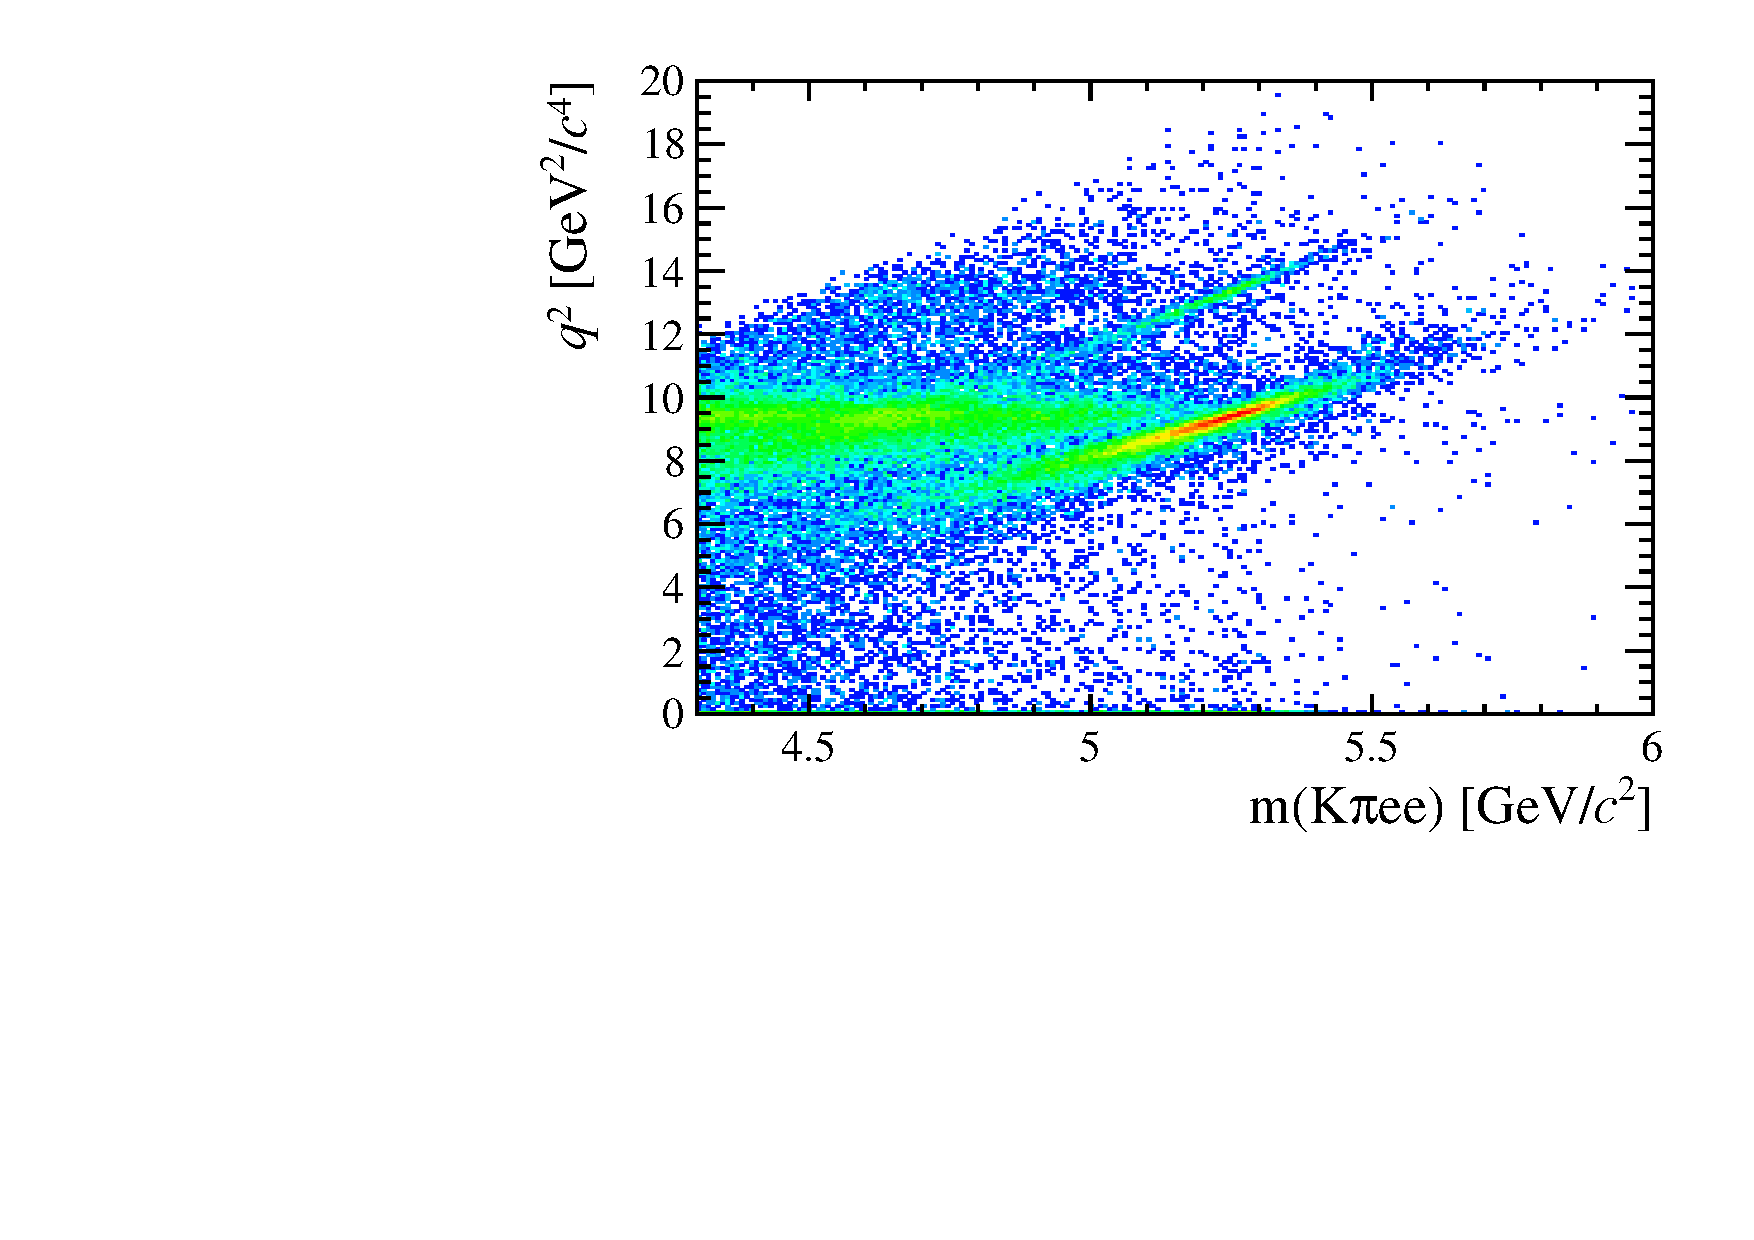
\includegraphics[width=1.\textwidth]{RKst/figs/electron_B0jpsi2D_selected.pdf}
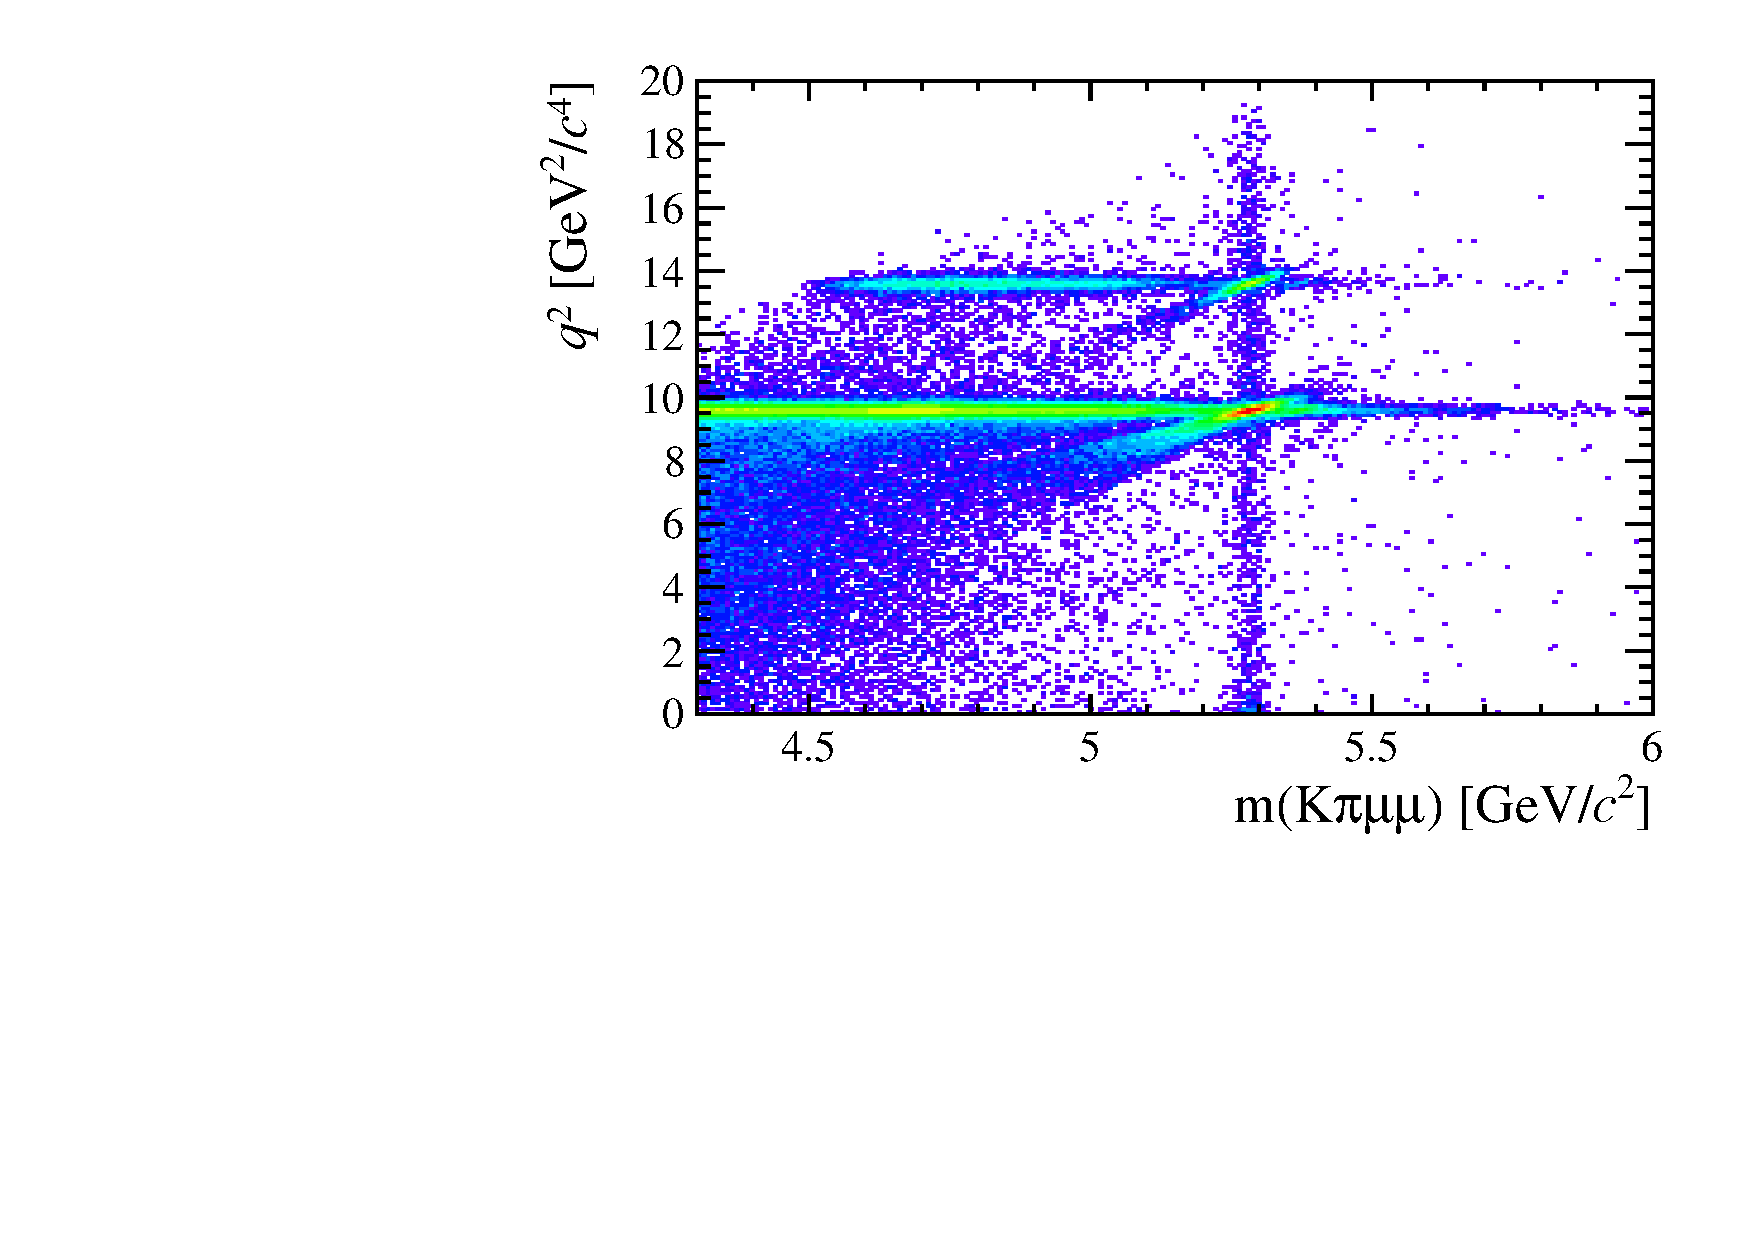
\includegraphics[width=1.\textwidth]{RKst/figs/muon_B0jpsi2D_selected.pdf}
\caption{Two-dimensional distributions of \qsq versus 4-body $m(K\pi\ell\ell)$
invariant mass for the electron (top) and muon (bottom) channels in 2012 data.}
\label{fig:2D_q2_B0mass}
\end{figure}


\subsection{Trigger and pre-selection }
\label{sec:RKst_trigstripping}

Events are triggered for the $\mu\mu$ and the $ee$ channels by the trigger lines
reported in Tab.~\ref{tab:RKst_triglines}, where the logical $and$ of L0, HLT1 and HLT2
lines is required and the logical $or$ of the lines on the same level. The candidates are
required to be triggered-on-signal (TOS) for most of the stages, namely it is required that the 
particle responsible for the trigger decision is one of the particles used to build the signal candidates.
Only for \verb!L0Global!, used in the electron case, a trigger-independent-of-signal (TIS) is required. 
%this is aimed to collect all the possible statistics for the electron channels, which are the most challenging.
The \verb!L0Muon! trigger requires hits in the muon detector, while \verb!L0Electron! and \verb!L0Hadron! use information
from the calorimeters; \verb!HLT1TrackAllL0! adds information from the trackers and
triggers if the L0 decision is confirmed; finally, \verb!HLT2Topo[2,3]BodyBBDT! uses a full reconstruction 
of the event and a neural network trained on candidates with a specific topology in order to detect specific decay structures.
%More information about the muon triggers can be found at Sec.~\ref{sec:Lb_trigger}.

\begin{table}[h!]
\begin{center}
\caption{Summary of the trigger lines used to select the $\mu\mu$ and the $ee$ channels.
Where not explicitly indicated, the lines are required to be TOS.}
\begin{tabular}{$c|^c|^c}
\rowstyle{\bfseries}
Trigger level & \boldmath{$\mu\mu$} candidates &  \boldmath{$ee$} candidates \\
\hline
\multirow{3}{*}{L0}     & 	\multirow{3}{*}{L0Muon}		&    	L0Electron	\\
				&							& 	L0Hadron\\
				&							& 	L0Global (TIS)\\
\hline
\multirow{2}{*}{HLT1}		&	Hlt1TrackAllL0				& \multirow{2}{*}{Hlt1TrackAllL0} \\
					&	Hlt1TrackMuon				&	 \\
\hline
\multirow{3}{*}{HLT2}		&	Hlt2Topo[2,4]BodyBBDT 		& Hlt2Topo[2,4]BodyBBDT \\
					& 	Hlt2TopoMu[2,4]BodyBBDT 	& Hlt2TopoE[2,4]BodyBBDT \\
					& 	Hlt2DiMuonDetachedDecision	&							\\
\end{tabular}
\label{tab:RKst_triglines}
\end{center}
\end{table}

For the electron channels the L0 lines have different properties, therefore the analysis 
is performed separately for three categories of events, depending on the L0 trigger that fired 
them. These categories are defined to be exclusive in the following way:
%
\begin{itemize}
\item {\bf L0E}: events triggered by at least one of the electrons in the signal candidate (\verb!L0Electron_TOS!);
\item {\bf L0H}: events triggered by at least one of the hadrons in the signal candidate and not in the L0E category \\
 (\verb|L0Hadron_TOS && !L0Electron_TOS|);
\item {\bf L0I}: events triggered by particles independent of any signal candidate and not included in the previous categories\\
(\verb|L0Global_TIS && !(L0Electron_TOS |\verb!|| L0Hadron_TOS)!).
\end{itemize}

The majority of the selected events falls into the L0E category, while
the L0H category is more efficient at low \qsq were the \Kstarz has higher momentum.
Because L0I is defined to be independent of the signal candidate, the corresponding
signal efficiency is the same in both the rare and resonant cases and therefore cancels in their ratio.

Candidates are then required to pass the kinematic and quality cuts summarised in Tab.~\ref{tab:RKstripping},
where the meaning of the variables was already explained in Sec.~\ref{sec:Lb_selection}.
Loose PID requirements are applied in pre-selection to limit the size of the samples, while tighter cuts 
are applied in a second stage. A wide mass window is kept around the \Bz peak so that
 the sideband can be used to train the multivariate classifier and to constrain the backgrounds.
%
%In the table $IP_{\chi_2}$ is defined as the projected distance from the vertex divided by its uncertainty, for example $IP^B_{\chi_2}(primary) > 4$ means
%that the B vertex is 2 standard deviations away from the primary vertex.
%Another quantity used is a pointing variable defined as the angle between the direction of the particle momentum and the flight direction from its mother vertex, called DIRA.
%This allows the selection of particles with well-defined primary vertices.
%%$GhostProb$ is the probability, estimated from the reconstruction algorithm, for the track to be a ghost. 
%Loose PID cuts are applied in preselection to limit the size of the samples, while tighter cuts are applied
%in a second stage. To quantify the PID of a particle the pion is used as a reference point and a Log-Likelihood
%variable is used. Therefore the {\verb PID } variable reported in the table is given in terms of the difference between
%the Log-Likelihood of the particle of a given type and a pion. This is called Delta Log-Likelihood (DLL).
%For example:
%\begin{equation}
%\verb!PID!_K = \text{DLL}_{K-\pi} = \log(\mathcal{L}_K) - \log(\mathcal{L}_\pi)
%\end{equation}
%
\begin{table}[]
\begin{center}
\caption{Summary of pre-selection requirements. Variables are defined in Sec.~\ref{sec:Lb_selection}. }
\begin{tabular}{$c^c}
\rowstyle{\bfseries}
Particle &  Requirements \\
\hline
%\multirow{2}{*}{ All final}
%       			&   track $\chi_2/\text{ndf} < 3$ \\
%       			&   {\verb GhostProb } $< 0.4$ \\
%\hline
$\pi$			& $\chisqip(primary) > 9$ \\      			
\hline
\multirow{3}{*}{K}
      			& {\verb PID }$_K > -5$ \\
       			& $\chisqip(primary) > 9$ \\
       			& {\verb hasRICH }  \\
 \hline
\multirow{4}{*}{ \Kstarz }
       			& $\pt > 500$ \mevc \\
       			& $|m_{K\pi} - m_{\Kstarz}^{PDG}| < 300$ \mevcc  \\ %300 in stripping but then we restrict it to 100
       			& $\chisqip(primary) > 9$ \\
       			& Origin vertex $\chisq/\text{ndf} < 25$ \\
\hline
\multirow{3}{*}{ $\mu$ }
       			& $\pt > 300$ \mevc \\
       			& $\chisqip(primary) > 9$ \\
       			& i{\verb sMuon }\\  %RequiresDet='MUON'
%       		& hasMuon \\
\hline
\multirow{4}{*}{ $e$ }
       			& $\pt > 300$ \mevc \\
       			& $\chisqip(primary) > 9$ \\
       			& {\verb hasCalo }\\ %RequiresDet='CALO'
       			& \verb!PID!$_e > 0$ \\
\hline
\multirow{4}{*}{ $\ell\ell$ }
				& $m_{\ell\ell} < 5500$ \mevcc \\
			  	& End vertex $\chisq/\text{ndf} < 9$ \\
			  	& Origin vertex $\chi^2$ separation $> 16$ \\
%			  	& $\chisqip(primary) > 0$ \\
\hline
\multirow{4}{*}{ $B^0$  }
 %      & $| m - m_{B^0}^{PDG}| < 600$ \mevcc  \\
       			& {\verb DIRA } $> 0.9995$ \\ 
       			& End vertex $\chisq/\text{ndf} < 9$ \\
     			& $\chisqip(primary) < 25$ \\
     			& Primary vertex $\chisq$ separation $> 100$ \\
\end{tabular}
\label{tab:RKstripping}
\end{center}
\end{table}
%
Track and vertex quality cuts are also applied using the $\chi^2_{track}/\text{ndf}$, 
{\verb GhostProb }, and $\chi^2_{vtx}/\text{ndf}$
variables. The {\verb GhostProb } quantity describes the probability of a track being fake.
By construction, cutting at 0.4 removes $(1 - 0.4)\cdot 100 = 60\%$ of fake tracks.
For details about the definition of the variables used see Ref.~\cite{Loki_twiki}.

\subsection{PID}
\label{sec:PID}

After pre-selection there still are high levels of background.
In particular, as the identification (ID) hypotheses for kaons and pions are not constrained, the samples
still contain multiple combinations for most candidates, therefore tighter PID requirements are applied.
In the LHCb analysis framework the particle identification probability can be quantified
using the ``{\verb ProbNN }$x$" variables~\cite{ProbNNs_pres}, where $x$ is a specific ID hypothesis: 
$p, K, \pi, e$ or $\mu$. These variables 
are the outputs of neural networks which use information from the calorimeters, the RICH detectors
the muon system and the tracking system. Unlike the DLL variables (see Sec.~\ref{sec:PID_perf})
the {\verb ProbNN } are bound from 0 to 1 and can be directly interpreted as probabilities; \emph{e.g.}
 {\verb ProbNNk } corresponds to the probability for a reconstructed particle to be a kaon.
%Two tunes of the {\verb ProbNN } variables, labelled V2 and V3, are available.
%Tune V3 was shown to be optimal for positive ID, while tune V2 was found to be optimal
%for background rejection and therefore it is used to quantify the mis-ID probability.
%
\begin{figure}[h!]
\centering 
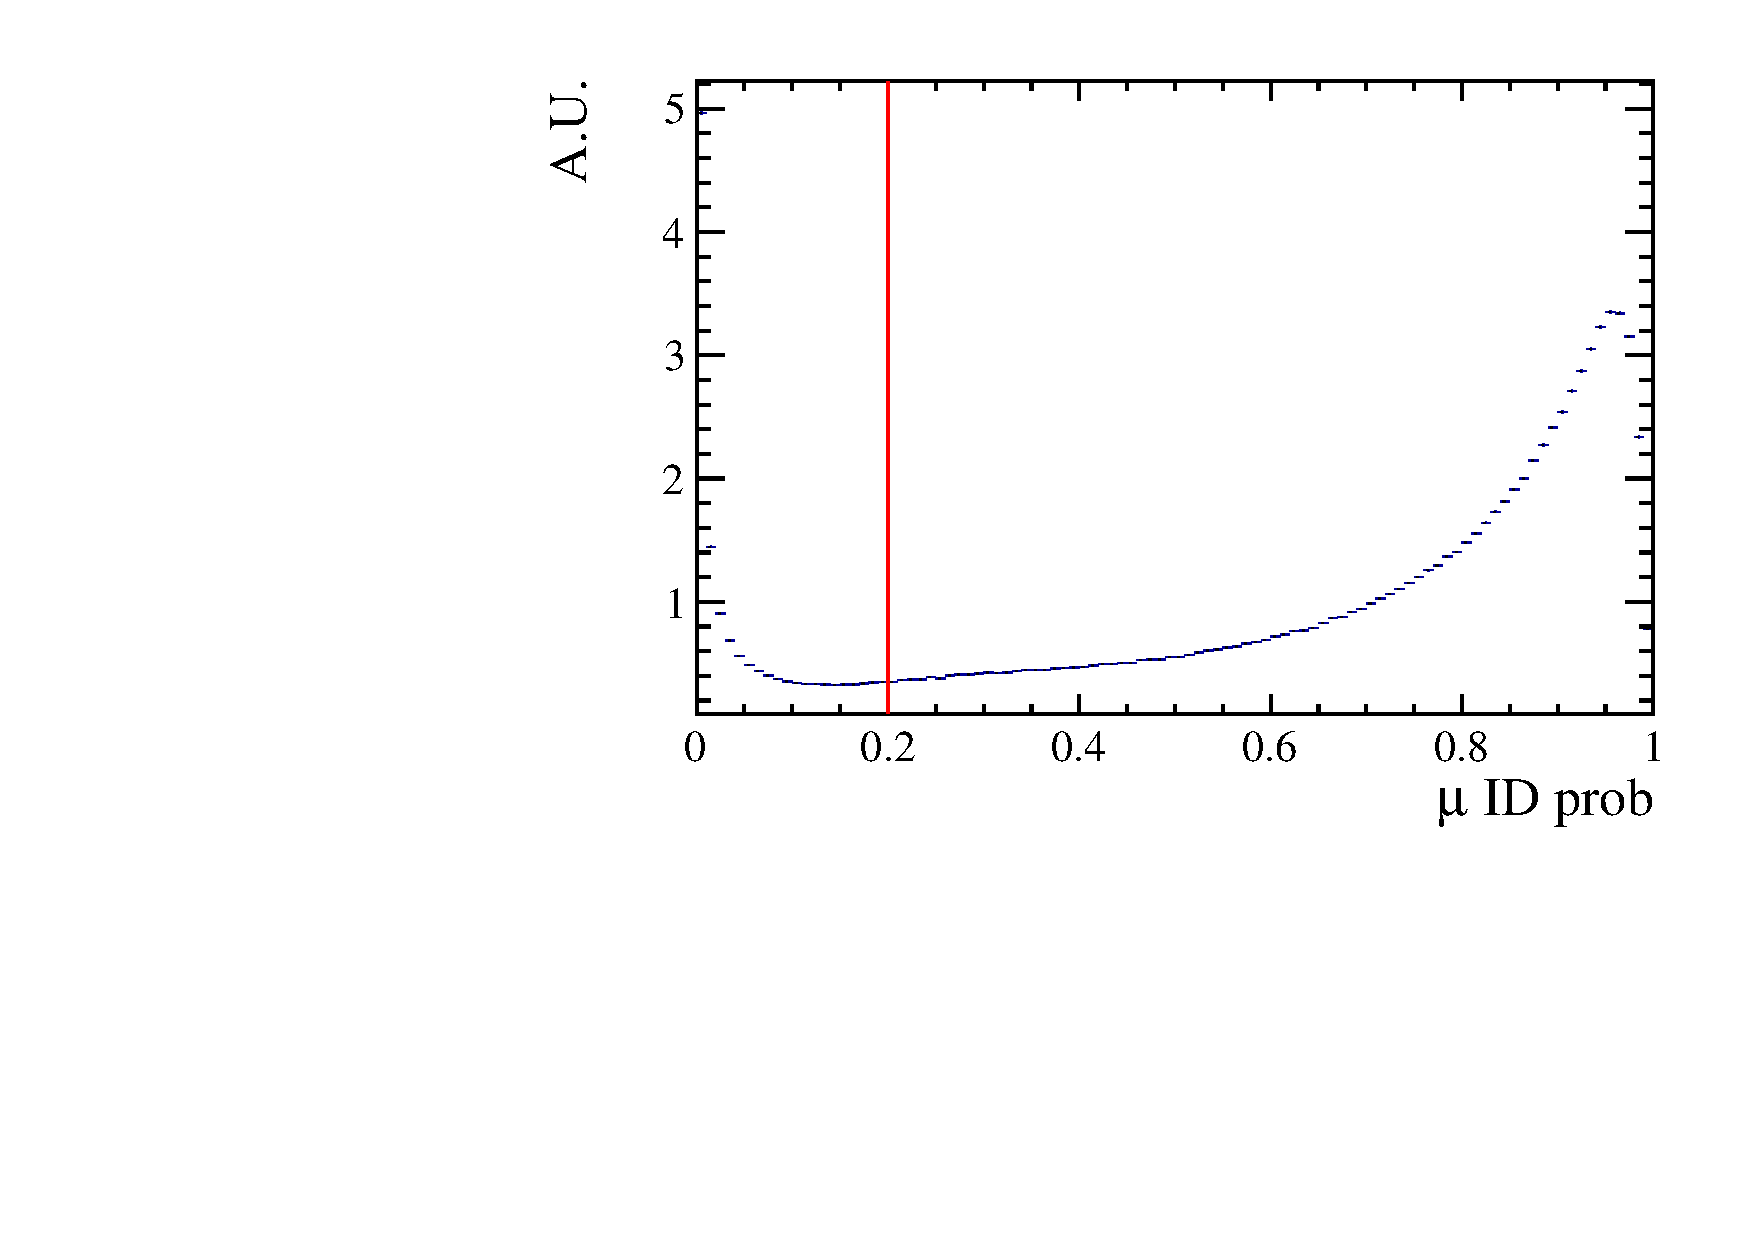
\includegraphics[width=0.48\textwidth]{RKst/figs/muon_PID.pdf}
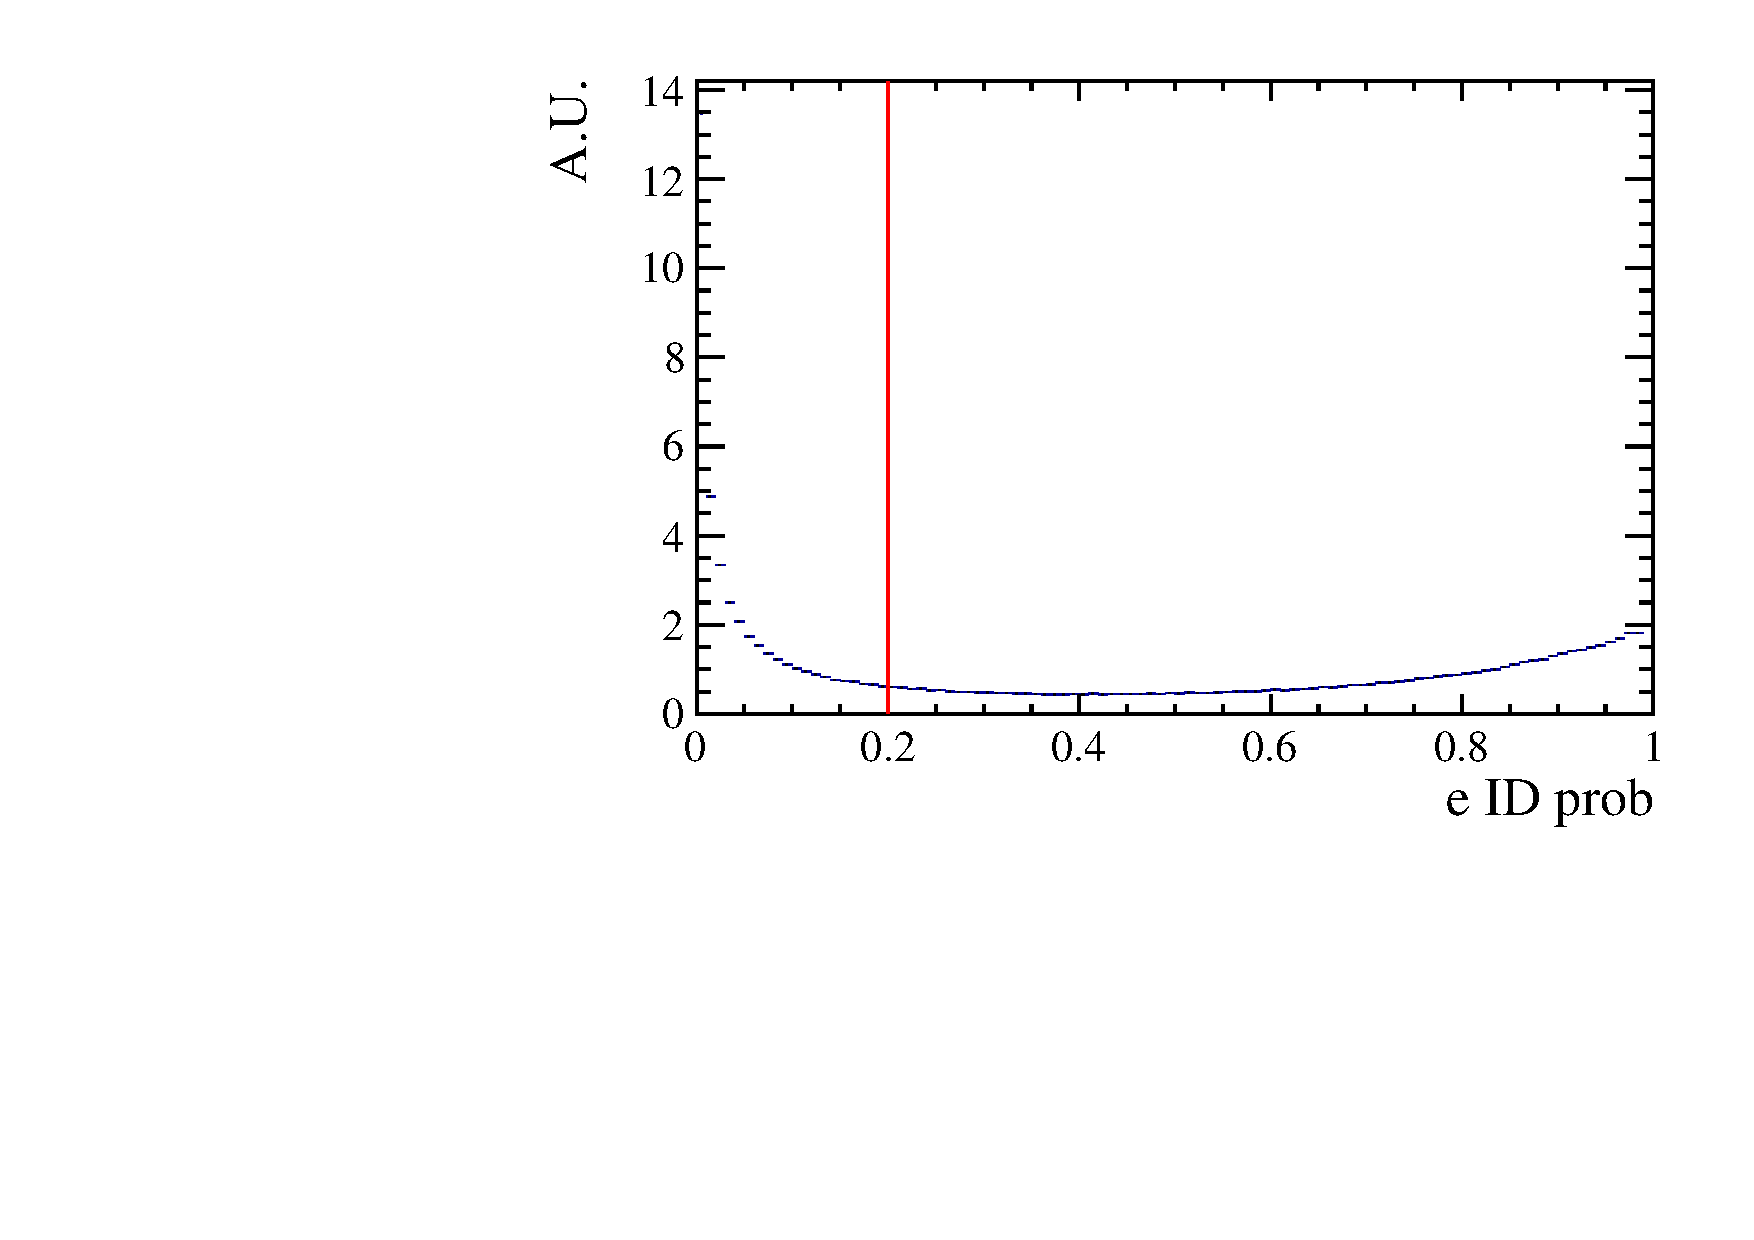
\includegraphics[width=0.48\textwidth]{RKst/figs/electron_PID.pdf}
\caption{Correct ID probability distributions for muons (left)
and electron (right) in 2012 data.}
\label{fig:e_mu_pid}
\end{figure}
%
\begin{figure}[h!]
\centering 
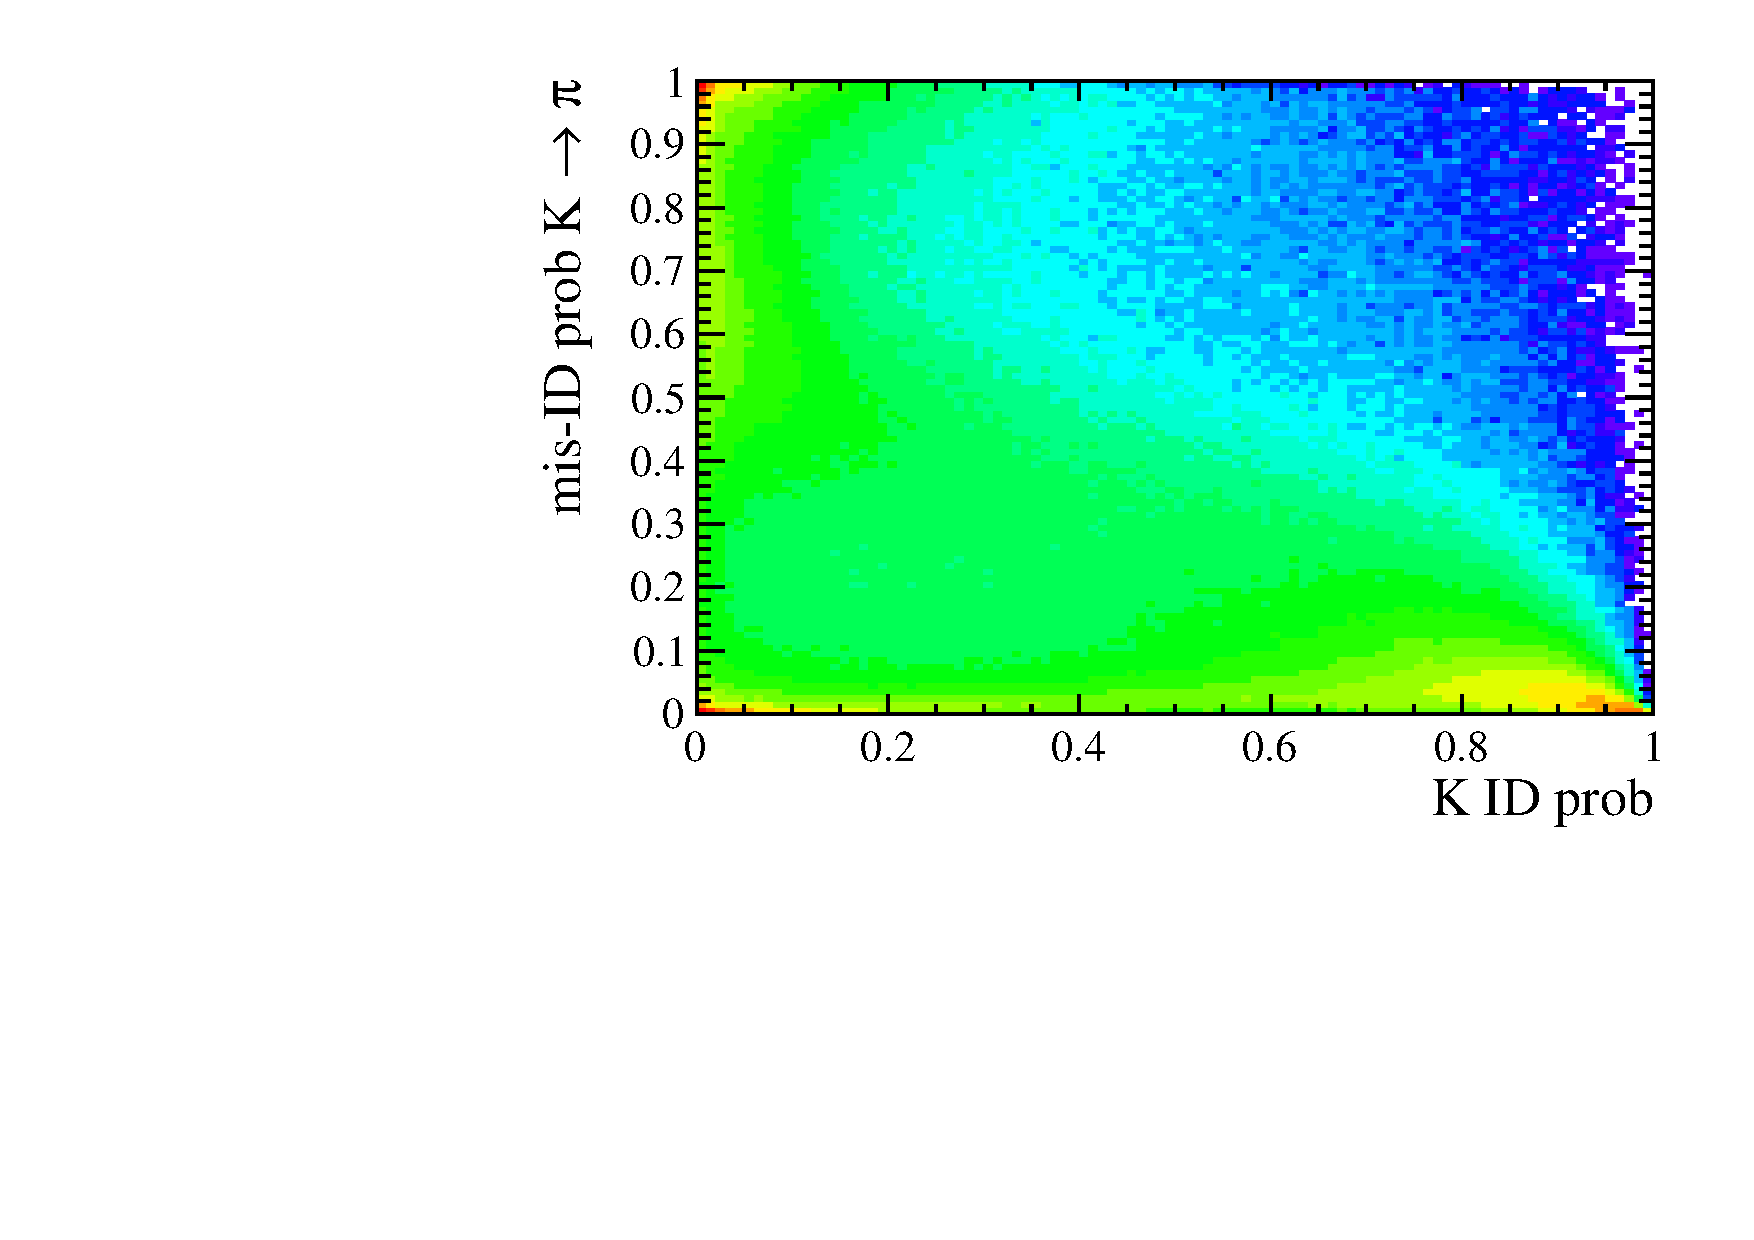
\includegraphics[width=0.48\textwidth]{RKst/figs/kaon_PID.pdf}
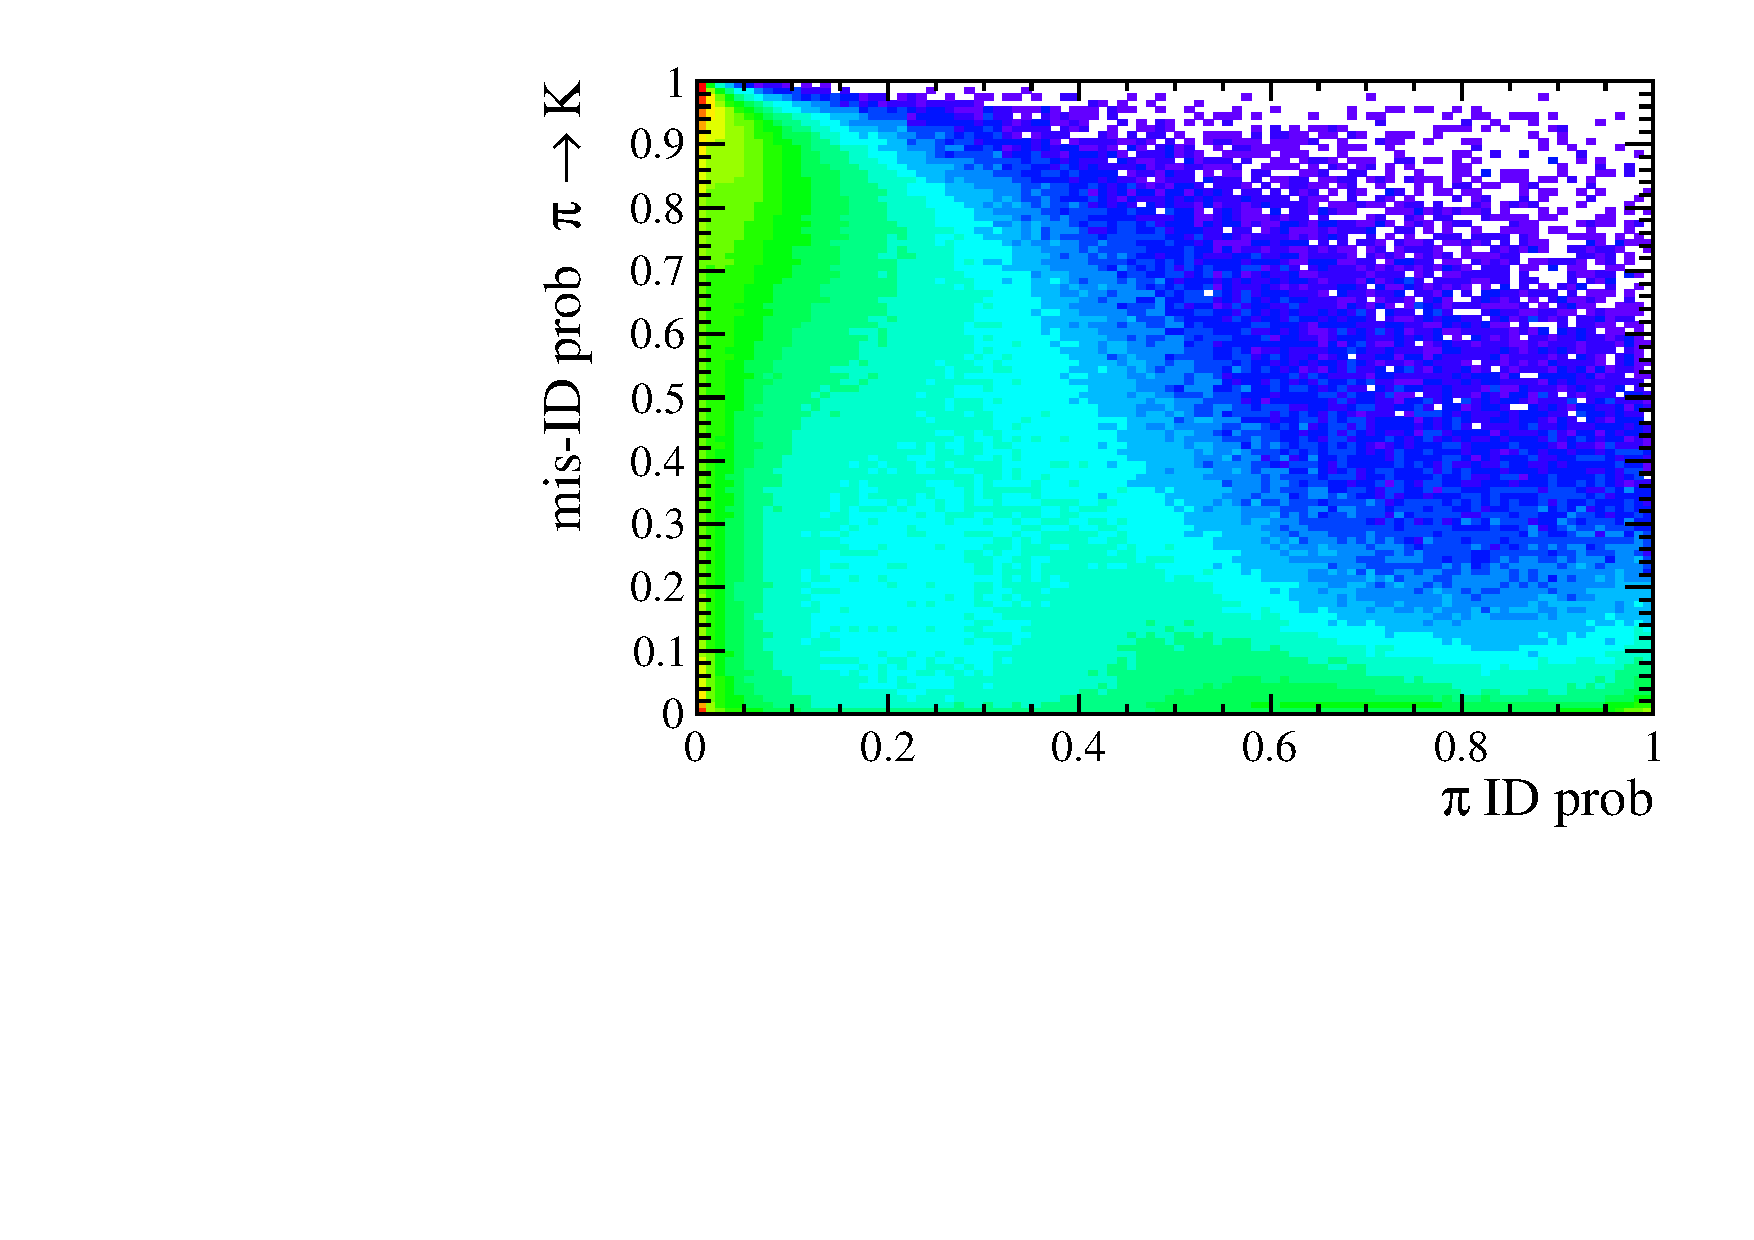
\includegraphics[width=0.48\textwidth]{RKst/figs/pion_PID.pdf}
\caption{On the horizontal axis of these plots is shown the correct ID
probabilities for kaons (left) and pions (right),
 while the vertical axes show the mis-ID probabilities.}
\label{fig:k_pi_pid}
\end{figure}

Figure~\ref{fig:e_mu_pid} shows probability distributions, {\verb ProbNNe } and {\verb ProbNNmu },
for the electrons and muons in the decay candidates, while Fig.~\ref{fig:k_pi_pid} shows the probabilities 
of correct identification and mis-identification of kaons and pions in a two-dimensional plane.
These plots are characterised by clear peaks at maximal ID probability and minimal mis-ID
probability, corresponding to particles to which a well defined identification can be assigned.
%
In order to maximise the power of the PID requirements, the probabilities for correct ID 
and mis-ID are combined and requirements imposed as:
%
\begin{center}
\begin{tabular}{lcl}
$\pi$     & \to  & $\verb!ProbNNpi! \times (1 - \verb!ProbNNk!) \times (1 - \verb!ProbNNp!) > 0.1$ \\
$K$      & \to  & $\verb!ProbNNk! \times (1 - \verb!ProbNNp! ) > 0.05$ \\ 
$\mu$  & \to  & $\text{min}(\verb! ProbNNmu!(\mu_1) , \verb! ProbNNmu!(\mu_2)\;) > 0.2$  \\
$e$      & \to  & $\text{min}(\verb! ProbNNe!(e_1), \verb! ProbNNe!(e_2)\;) > 0.2$ \\
%$\pi$ &\to  & $\verb!ProbNNpi-V3! \times (1 - \verb!ProbNNk-V2!) \times (1 - \verb!ProbNNp-V2!) > 0.1$ \\
%$K$   &\to  & $\verb!ProbNNk-V3! \times (1 - \verb!ProbNNp-V2! ) > 0.05$ \\ 
%$\mu$ &\to  & $\text{min}(\verb! ProbNNmu-V3! , \verb! ProbNNmu-V3 !) > 0.2$  \\
%$e$   &\to  & $\text{min}(\verb! ProbNNe-V3! , \verb! ProbNNe-V3 !) > 0.2$ \\
\end{tabular}
\end{center}
%
In the first formula, for example, {\verb ProbNNpi } is the probability of correctly identifying the
pion as a pion, while {\verb ProbNNk } is the probability of mistaking it for a kaon.
Therefore by maximising the quantity ``{\verb ProbNNpi } $\times$ (1 - {\verb ProbNNk })",
one can maximise the correct ID probability and minimise at the same time the mis-ID probability.
In this example, the probability for mistaking the pion as a proton is also used.
%In the kaon case we do not use requirements on the $K\to\pi$ mis-ID probability
%because this cut was found to be unacceptably inefficient.


\subsection{Peaking backgrounds }

Backgrounds due to specific decays usually peak in some variable because of their
distinctive kinematic properties and therefore they can be removed without significant
efficiency loss for the signal. The following sections describe the main sources of peaking background.
The same requirements are applied to the muon and electron channels, unless stated otherwise.

\subsubsection{Charmonium vetoes}

Charmonium resonances such as \jpsi and \psitwos peak in \qsq.
The choice of \qsq binning described in Sec.~\ref{sec:RKst_q2_choice}
constitutes a natural veto for these decays. Simulated events are used
to check if resonant candidates leak inside the \qsq intervals chosen for
the rare channel analysis. For the muon channels the leakage is negligible
as the peaks are sharper due to the better momentum resolution and because muons 
emit fewer bremsstrahlung photons, resulting in shorter radiative tails.
The electron channels are characterised by a poorer energy resolution and an increased 
radiation of bremsstrahlung photons, yielding long tails at low \qsq.
Analysing simulated events it was found that 1.3 -- 2\% (depending on
the trigger category) of \mbox{$\Bz\to\Kstarz(\jpsi\to\ee)$} candidates leak into the 
$1.1 < \qsq < 6$~\gevgevcccc interval and 1.8\% of \psitwos events leak above 
15~\gevgevcccc. The contribution from these candidates is modelled in the fit. 


\subsubsection{$\phi$ veto}

A kaon from the decay $\Bs \rightarrow \phi \ll$, where the $\phi$ decays in two kaons,
can be mis-identified as a pion and therefore causes the $\phi$ to be reconstructed as a $\Kstarz$. This results in
a candidate with a value of $m(K\pi)$ that is less than the nominal \Kstarz mass but still high enough to
pass the selection requirements. Figure~\ref{fig:phiplots} (left) shows a plot of $m(K\pi)$ versus
$m(K\pi \mu\mu)$, where the kaon mass hypothesis is assigned to the pion. A peak can clearly be seen
around the (\Bs,$\phi$) mass.
To remove this background only candidates with $m_{K(\pi\rightarrow K)} > 1040$~\mevcc~are selected.
This results in a $\sim98\%$ background rejection while keeping a $\sim99\%$ signal efficiency.
%This cut could be further optimised using PID information. On the other hand LHCb simulation 
%struggles modelling the PID variables correctly. Therefore using PID in these cuts would
%add systematic uncertainties without significantly improving the signal efficiency which is already 99\%.
\Bs decays such as $B_s \rightarrow \phi \Kstarz$ could also constitute a background when the $\phi$ decays 
into two leptons but the branching fraction of this decay is small compared to the previous case.
Furthermore, this contribution is already taken into account by the choice of the \qsq intervals (see Sec.~\ref{sec:RKst_q2_choice}).

\begin{center}
\begin{figure}[h!]
\centering 
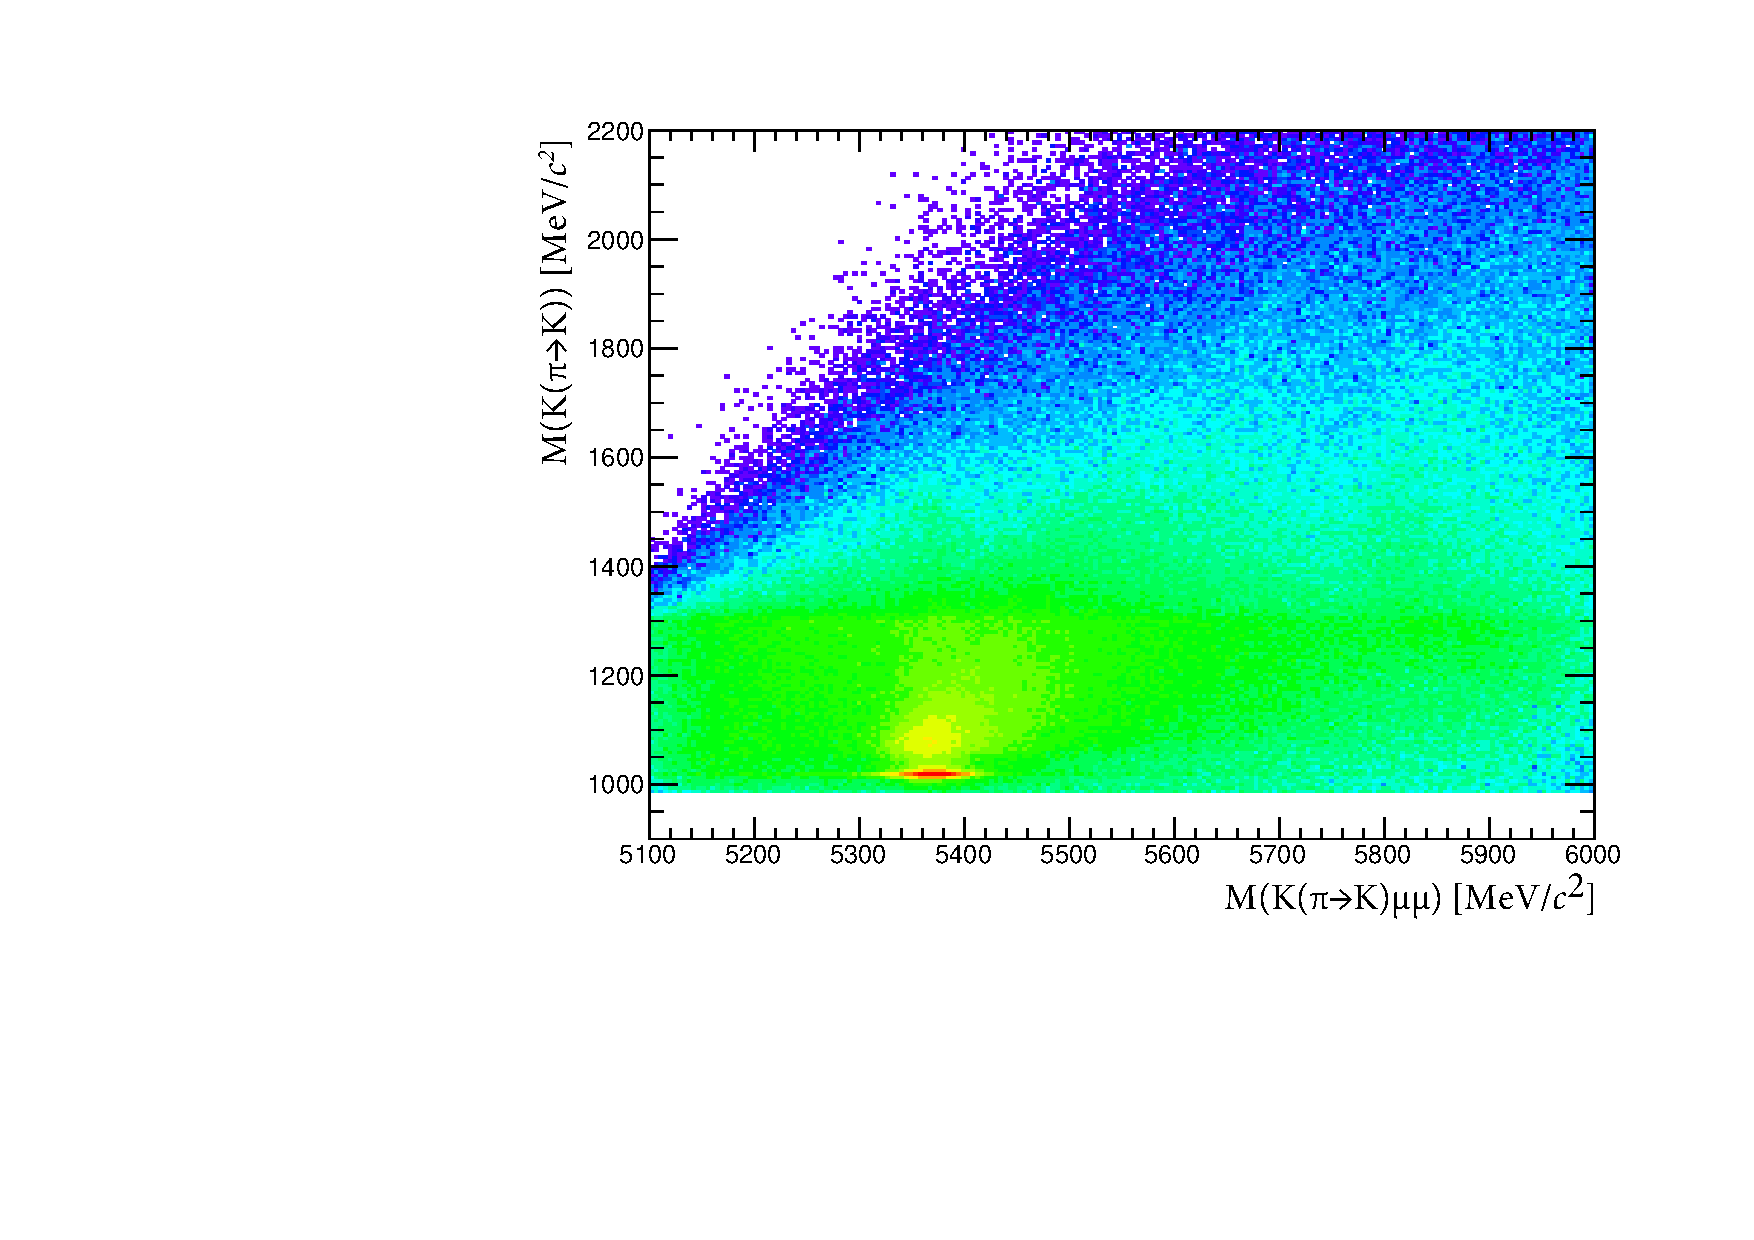
\includegraphics[width=0.49\textwidth]{RKst/figs/Background/phi.pdf}
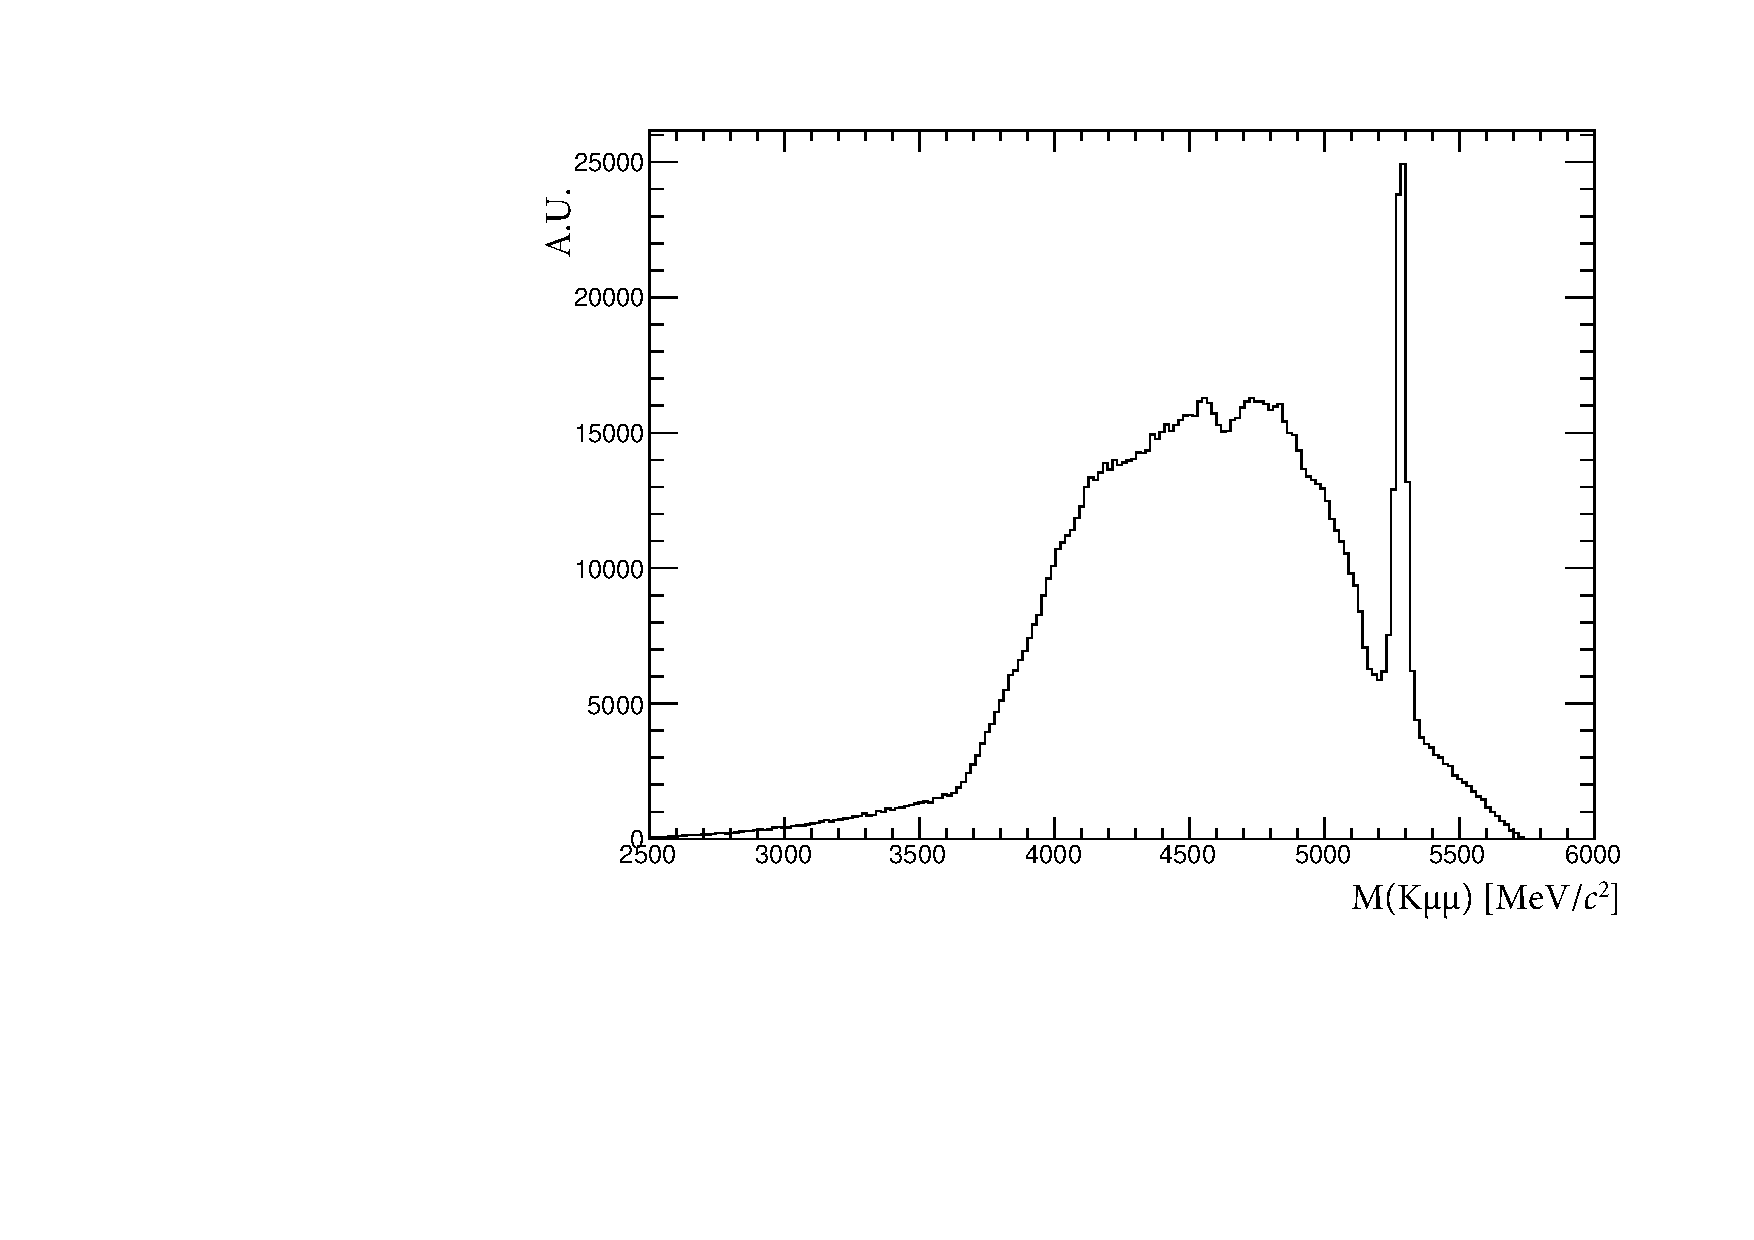
\includegraphics[width=0.49\textwidth]{RKst/figs/Background/Kmumu.pdf}
\caption{ (left) Distribution of data candidates as a function of the variables $(m_{K(\pi\rightarrow K)})$ 
and $(m_{K(\pi\rightarrow K)\mu\mu})$, where $\pi\rightarrow K$ means that the kaon mass hypothesis 
is assigned to the pion. (right) The invariant mass distribution of the three-body system $(K\mu\mu)$,
where the peak due to the $B^+ \to K^+ \mumu$ decay is visible. }
\label{fig:phiplots}
\end{figure}
\end{center}


\subsubsection{$\Bu \to K^+ \ll$ plus a random pion}

$\Bu \to K^+ \ll$ decays can contaminate the upper \Bz mass sideband if they are combined
with a soft pion from elsewhere in the event and therefore reconstructed as a \Bz decay.
Similarly a kaon can be mis-identified as a pion and combined with another kaon in the event.
Figure~\ref{fig:phiplots} (right) shows the invariant mass distribution of the three-body ($K\mumu$) system,
$m(K\mu\mu)$. This is characterised by a narrow peak at the $\Bu$ mass. Since these
candidates have $m(K\pi\ell\ell) > 5380$~\mevcc~there is no contribution under the \Bz peak,
but they can cause problems when using sidebands candidates to train the neural network.
An effective veto for this decay was found to be max$(m_{K\ell\ell},m_{(K\to\pi)\ell\ell}) < 5100$~\mevcc,
which results in a $\sim95\%$ background rejection while keeping $\sim99\%$ signal efficiency.

\subsubsection{$\Lambda_b$ decays}

$\Lb\to\jpsi\Lz$ decays are unlikely to be reconstructed as $\Bz \to \Kstarz \ll$ because
the \Lz is long-lived and decays further in the detector with a separate vertex.
%Nevertheless, simulated events were used to check how many 
The number of candidates falling into the \Bz samples was estimated using simulation and found to be negligible. 
In contrast, the $\Lb\to\jpsi pK$ decay channel can contribute more easily, when the proton is mis-identified as a kaon.
In fact, the $m(pK)$ is above the \Lz threshold and therefore they must come from $\Lz^*$ resonances, 
 which are not long-lived. This background is already reduced by the PID requirements but a non-negligible contribution 
 is still expected, and cannot be easily removed due to its broad shape. It is therefore modelled in the fit.

\subsubsection{\decay{\Bd}{(\Dm\to K \en \overline{\nu})\ep\nu} }

The \decay{\Bd}{\Dm\ep\nu} decay, where the \Dm in turn decays semileptonically to $\Kstarz\en\nu$ has the same final particles
as the \BdToKstee decay plus two neutrinos which are not reconstructed. This decay has a branching ratio four orders of magnitude
larger than \BdToKstee in the low-\qsq region and it may pass the selection requirements when the two neutrinos have low momentum. 
%This cut, developed for the angular analysis, 
To reduce the level of this background the angle $\theta_\ell$ is used, which is defined as the angle between the direction of the \ep (\en)
in the di-electron rest frame and the direction of the di-electron in the \Bd (\Bdb) rest frame. 
Low momentum neutrinos demand the \Dm and the \ep to be almost back-to-back in the \Bd rest frame giving the \ep a relatively
high energy compared to the \en. As a consequence, the direction of the \ep is close to the direction of the di-electron pair, thus the
$\theta_\ell$ angle is close to zero. In fact the distribution of background candidates, obtained imposing the invariant mass cut
$m(K\pi ee) < 4800$~\mevcc, is asymmetric towards extreme $\cos \theta_\ell$ values as it can be seen in Fig.~\ref{fig:Denu_background}. 
The requirement $|\cos \theta_\ell\,|< 0.8$ is used but is not applied in the high-\qsq case as the variable has reduced discriminating power.
%The percentage of \BdToeeKst signal events lost applying this cut is quite low, about $10\%$ according to MC. 
In the muon channels, the background from \decay{\Bd}{(\Dm\to K \mun \overline{\nu})\mup\nu} decays remains outside 
of the invariant mass window used for the fits.

\begin{figure}[t!]
\centering
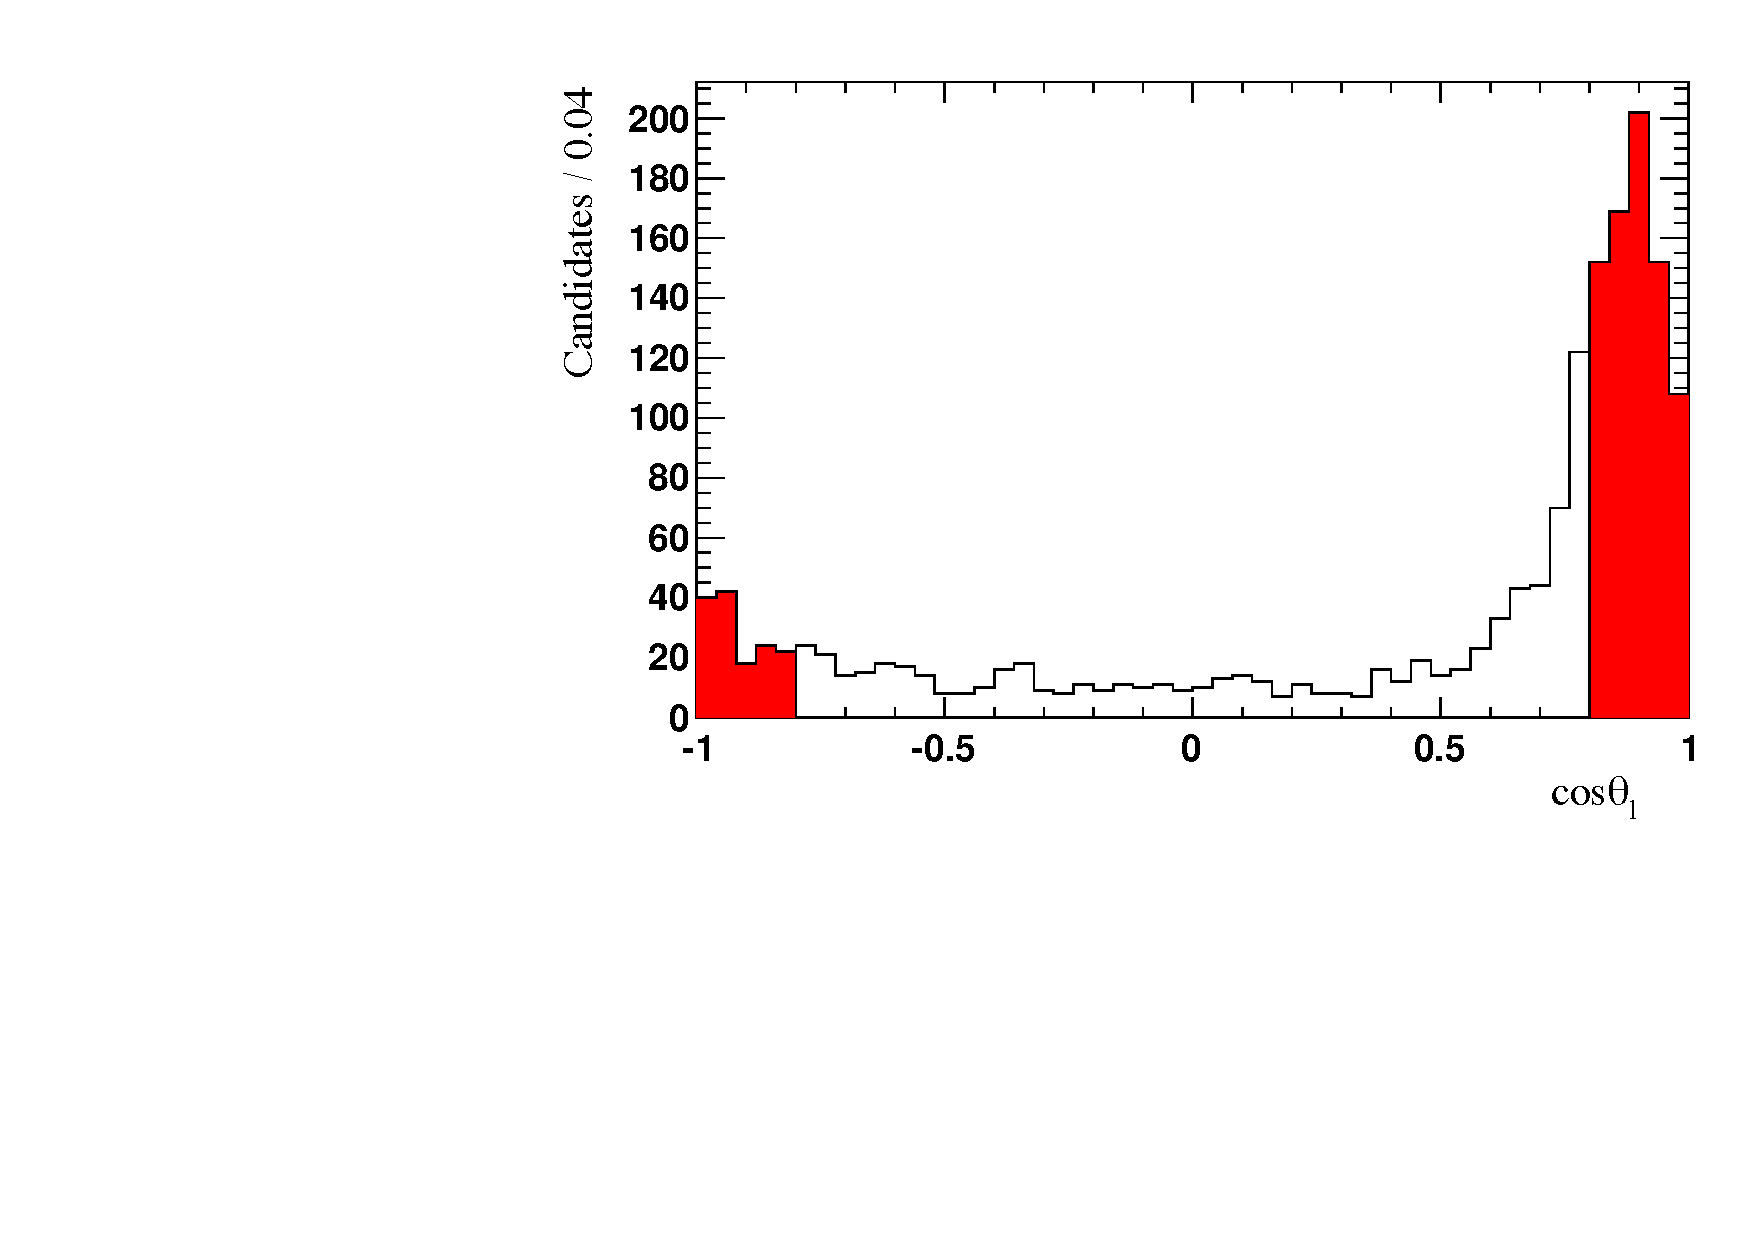
\includegraphics[width=0.49\textwidth]{RKst/figs/misreco/CosThetaL_background.pdf}
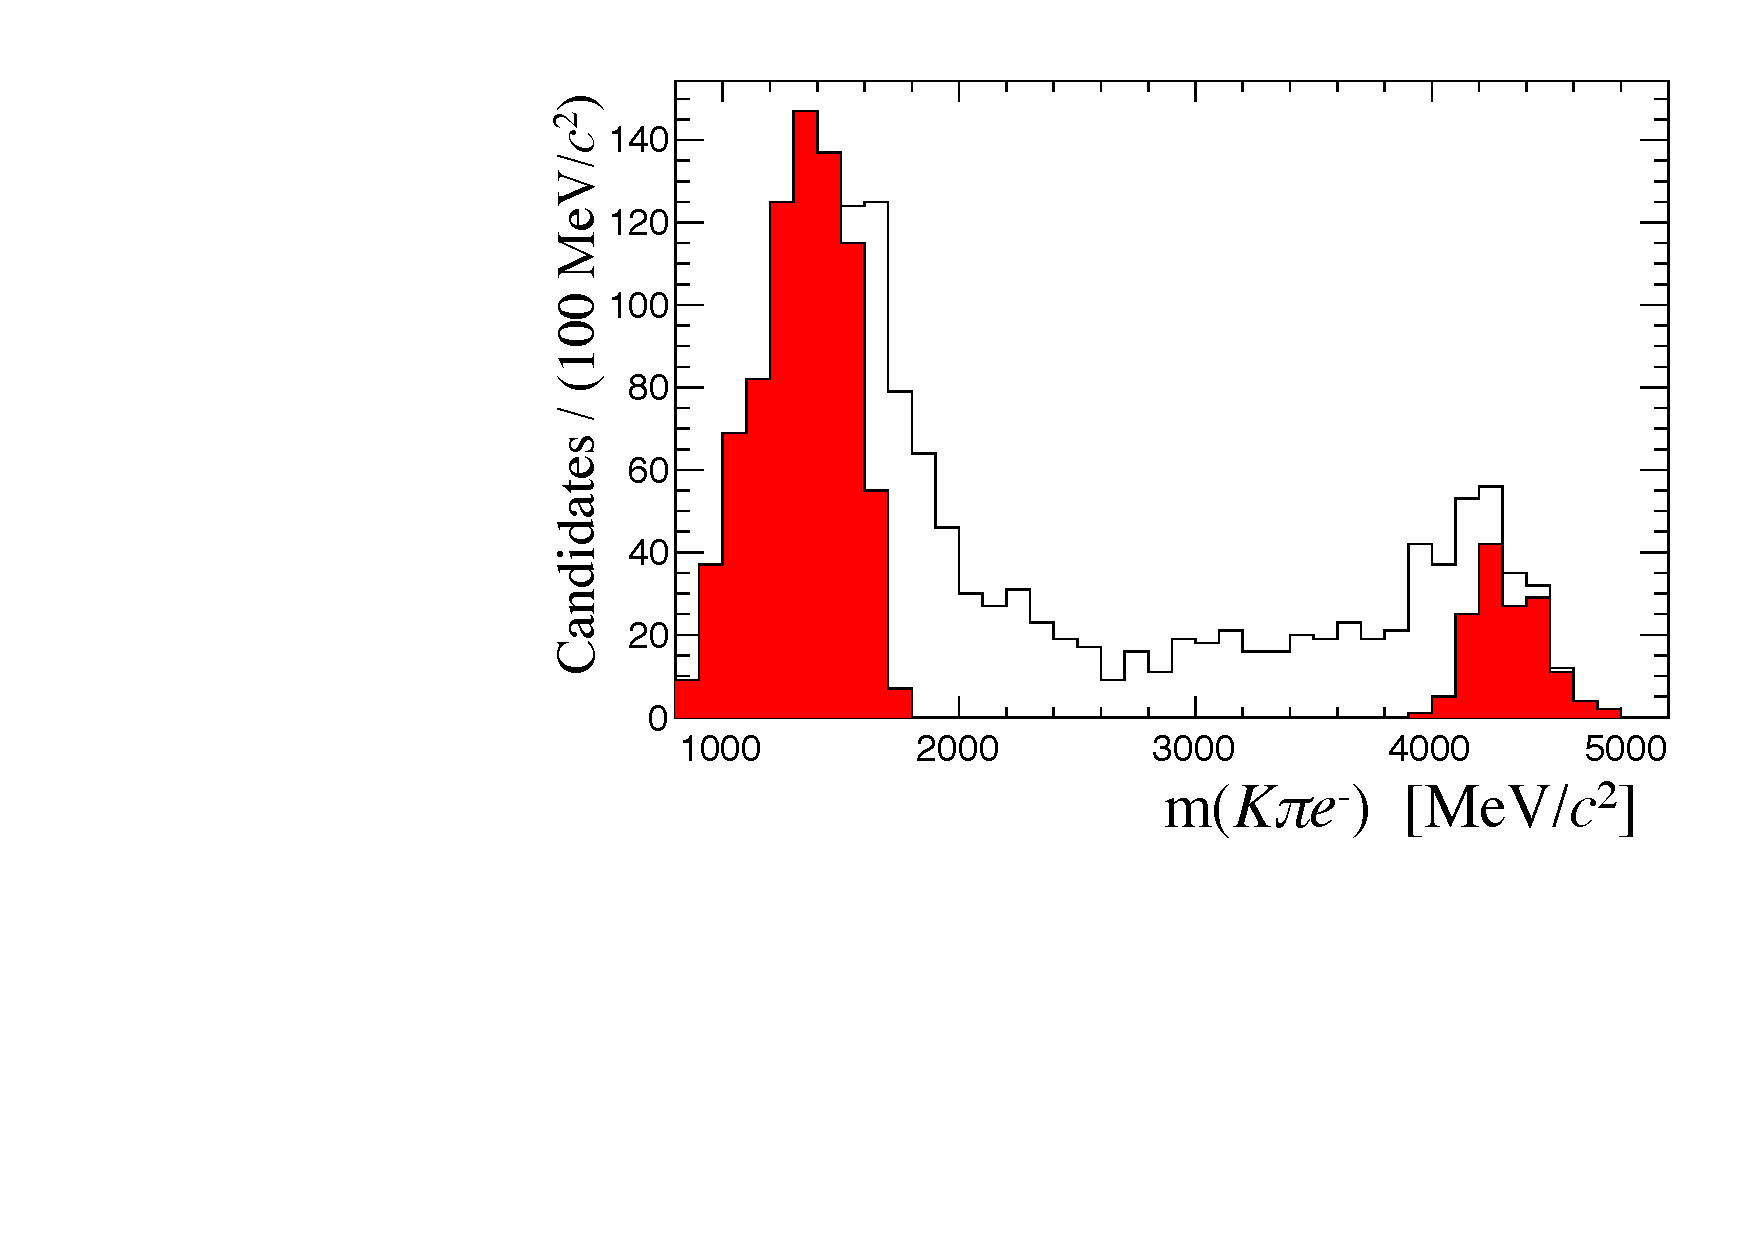
\includegraphics[width=0.49\textwidth]{RKst/figs/misreco/KstareMass_background.pdf}
\caption{Distribution of (left) $\cos \theta_\ell$ and of (right) the $m(K\pi e^-)$ invariant mass, where the \decay{\Bd}{(\Dm\to K \en \overline{\nu})\ep\nu} background is selected by requiring $m(K\pi ee) < 4800~\mevcc$. The red distribution highlights candidates with $| \cos \theta_\ell\,| > 0.8$.}
\label{fig:Denu_background}
\end{figure}

\subsubsection{\BdToKstGee}

For the low-\qsq region, a potentially dangerous peaking background is due to the \BdToKstG decay followed by a conversion
of the photon in the detector. The branching fraction of \BdToKstG has been measured to be \mbox{\BF~= $(4.33 \pm 0.15)\times 10^{-5}$} and, 
when the photon converts to an electron and a positron, has similar characteristics to \BdKstee. 
In \lhcb around 40\% of photons convert before the calorimeter. Although only $\sim 10\%$ of these convert
in the VeLo and are reconstructed as long tracks, the resulting \Bd mass should peak under that of the signal. 
This signal-like background is reduced effectively by the choice of the lower bound for the low-\qsq interval which corresponds to 
$m(ee)=20$~\mevcc. Furthermore, the \ee~pair from \BdToKstGee has a vertex at the point where the photon converts, but it may 
still be reconstructed as originating from the \Bd decay if the \ee~vertex position is determined with a large uncertainty. 
Therefore a requirement is applied on the uncertainty of the reconstructed $z$-coordinate of the \ee~pair: $\sigma_z(\ee) < 30$~mm.
%The contamination from the background is estimated in the following way: a quasi pure sample of \BdToKstGee is selected requiring that the 
%reconstructed invariant mass window for the \epem pair is smaller than 5~\mevcc. The event yield obtained on data ($881 \pm 39$ events)
%s used to rescale the prediction of the LHCb MC to get rid of problems related to an absolute prediction. 
Simulated events are used to predict the contamination from \BdToKstGee decays in the signal region which is found to be $(3.2\pm1.6)\%$.
%1.6 \%. 
%Finally as pointed out in ~\cite{LHCb-ANA-2014-009}, a conservative correction to take into account the mis-modelling 
%of the Bethe-Heitler process in Geant4 is further applied. The contamination is estimated to amount to  $(3.2\pm1.6)\%$ of the signal yield. 



\subsubsection{Other peaking backgrounds}

%A possible background could come from $\Bz \to\Kstarz\gamma$ decays where the photon converts
%into two electrons while traversing the detector. In LHCb, around 40\% of photons convert before the calorimeter,
%but only a small fraction of these, $\sim 10\%$, are reconstructed. Furthermore these events fall
%into a \qsq region well below the intervals considered in this analysis and their contribution is therefore negligible.

A potential contamination from $\Bz \to\Kstarz\eta$ and $\Bz \to\Kstarz\pi^0$, where the $\eta$ and the pion decay into
two photons, was considered and found to be small.
Furthermore, a potentially dangerous background could come from candidates where the
identity of the kaon and the pion are swapped as these candidates peak under the signal.
Although their contribution is found to be small, 0.5\%, the effect of their modelling in the fit
is taken into account when evaluating the systematic uncertainties. Finally, charmonium decays where 
the identity of the kaon, or the pion, and one of the muons  are swapped is are rejected by requiring that the 
hadron-$\mu$ invariant mass $m((h \to \mu)\mu)$, where the muon mass hypothesis is assigned to the hadron, 
is not compatible with a \jpsi (\psitwos) resonance: $|m((h\to \mu)\mu)-m_{\jpsi, (\psitwos)} | > 60$~\mevcc.

\subsection{Partially-reconstructed background}
\label{sec:RKst_peaking_Dchains}

Partially-reconstructed candidates are defined as decays where one or more particles in the final state are not reconstructed,
resulting in $m(K\pi\ell\ell)$ values smaller than the mass of the \Bz, but with tails that can still contaminate the signal sample.
Sources of partially-reconstructed background are decays involving higher hadronic states such as 
\decay{\Bz}{(Y\to\kaon\pi X)(\jpsi\to\epem)}, where $X$ represents at least one particle that is not reconstructed. 
The $Y$ state can be a \Kstar resonance as well as \D mesons that decay semileptonically, as explained in the previous sections.
For the resonant channels, an additional source of partially-reconstructed 
background comes from decays of higher \ccbar resonances, \decay{\Bz}{(\Kstarz\to K\pi)(Y\to(\jpsi\to\epem)X)}.

To reject such backgrounds, the 4-body invariant mass $m(K\pi\ell\ell)$ is recalculated using 
\verb!DecayTreeFitter! to impose vertex constraints. For the resonant case this also includes constraining the invariant mass 
mass of the dilepton pair to that on the \jpsi; in this case the 4-body mass is denoted as $m(K\pi\ell\ell)_{\jpsi}$. This constraint 
pushes partially-reconstructed candidates towards low $m(K\pi\ell\ell)_{\jpsi}$ values, resulting in no contamination above 5150~\mevcc. 

This requirement is implicitly applied for the muon channels by the definition of the invariant mass fit-windows. For the electron channels,
the requirement $m(K\pi\ell\ell)_{\jpsi(\psitwos)} > 5150~\mevcc$ is explicitly applied to select the $\jpsi(ee)$ and $\psitwos(ee)$ samples.
However, the vertex constraint alone is not sufficient to remove all background in the electron rare decay channels.
Furthermore, to correctly model the long radiative tails of the mass shapes, a fit region that extends 
down to 4500~\mevcc~is necessary. As a consequence the partially-reconstructed background is still relevant
for the electron rare channels and extends below the signal peak. For this reason this background is modelled 
in the fit for the rare channels (for details see Sec.~\ref{sec:RKst_misreco_fit}).


%Mis-reconstructed background is defined as decays where one or more particles are not reconstructed.
%The candidates built from these decays tend to have a low 4-body invariant mass as some particles are not reconstructed.
%A source of mis-reconstructed background is due to cascade decays with a \Bz decaying semileptonically
%into a $D$ meson which also decays semileptonically, e.g. $\Bz\to D^{-} \ell^+ \bar{\nu_\ell}$
%followed by $D^{-} \to \Kstarz \ell^- \nu_\ell$. 
%This is in general true for any partially reconstructed background from $B$ decays.
%
%To remove this background in the muonic channels, the 4-body $m(K\pi\mumu)$ invariant mass is recalculated
%with a kinematical fit using the \verb!DecayTreeFitter! package. In the resonant case this includes a constraint of the dilepton
%mass to be the \jpsi nominal mass and in both rare and resonant cases each particles is constrained to point to 
%its origin vertex. This constraint has the effect of pushing the misreconstructed events far from the \Bz peak.
%Therefore, to avoid this background, it is sufficient to limit the analysis to 4-body invariant masses
%above 5150~\mevcc.

%In the electron case it is instead important to fit a wider mass window to correctly constrain the background
%therefore one cannot eliminate this mis-reconstructed background which is then modelled in the fit
%(for details see Sec.~\ref{sec:RKst_misreco_fit}).

\subsection{Bremsstrahlung corrected mass}
\label{sec:HOP}

For the electron channels it is particularly difficult to separate partially-reconstructed and combinatorial background from the 
long radiative tail of the signal. Additional information to reduce these backgrounds is provided by the kinematics of the decay: 
the transverse momentum of the \Kstarz and dielectron, defined relative to the flight direction\footnote{The flight direction is defined 
using the primary and the decay vertices.} of the parent \Bz meson, should be equal and opposite, as illustrated in Fig.~\ref{fig:schemaHOP}.
%\cite{LHCb-INT-2015-000}.
%In fact for the \Bz daughters, the \Kstarz and the dielectron, the momentum components orthogonal to the flight 
%direction\footnote{The flight direction is defined using the primary and the decay vertices.} of the \Bz meson, \pt, 
%should cancel out as described by the sketch shown in Fig.~\ref{fig:schemaHOP}.
\begin{figure}[b]
 \centering
    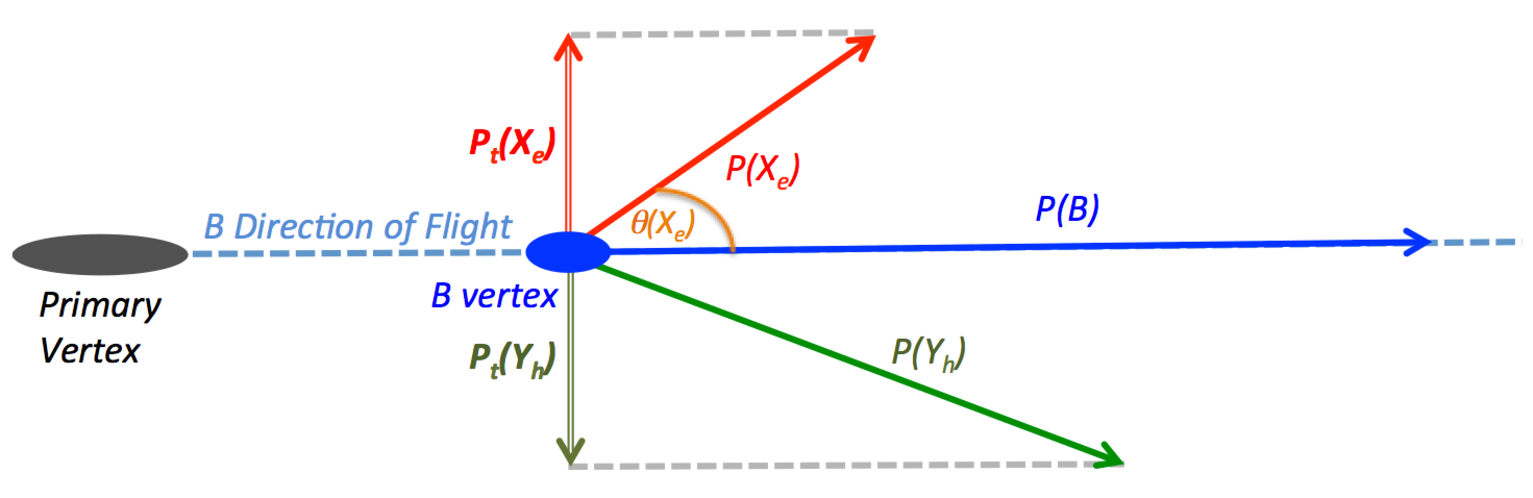
\includegraphics[width=0.9\linewidth]{RKst/figs/HOP/schemaHOP.pdf}
  \caption{ Schematic of the kinematic of a $B \to Y_h X_e$ decay, highlighting the quantities relevant for the 
  definition of the bremsstrahlung correction factor, $\alpha$.}
  \label{fig:schemaHOP}
\end{figure}

The ratio between the transverse momenta, \pt, of the \Kstarz and the dielectron pair, $\alpha = \pt(\Kstarz) / \pt(\ee)$, can be used 
to check this hypothesis. When $\alpha$ deviates from one, some energy is missing in the final state. 
For signal candidates, the missing energy is most likely carried away by bremsstrahlung photons emitted
by the electrons. Therefore we can use $\alpha$ to correct the electron momentum as $\ptot_{\textrm{corr}}(\ee) = \alpha \cdot \ptot(\ee)$.
Since bremsstrahlung photons are predominantly emitted in the direction of the electron, the same $\alpha$ correction can
be also applied to the longitudinal component of the dielectron momentum.
In contrast, the missing particles in partially-reconstructed background candidates are not necessarily emitted in the
direction of the electrons, and therefore this correction does not work properly.
A similar argument applies to the combinatorial background. 

The corrected momenta can be used to re-calculate the invariant mass of the \Bz candidate, which in the following will be
called Bremsstrahlung Corrected Mass, \mbcm. The resolution of \mbcm depends on the quality of the vertex reconstruction
and on the \Bz lifetime, and degrades as a function of \qsq. Figure~\ref{fig:hop} shows the dependence of the \Bz $\chisq_{\rm FD}$ 
(flight distance $\chisq$) as a function of \mbcm in the considered \qsq regions. 

As the correction factor is not meaningful for backgrounds this leads the candidates to spread out making \mbcm 
a discriminating variable between signal and background. A two-dimensional cut is adopted
%
$$\mbcm > a_{\rm BCM} + b_{\rm BCM} \cdot \log(\chisq_{\rm FD}),$$
%
where the $a_{\rm BCM}$ and $b_{\rm BCM}$ coefficients are optimised as described in Sec.~\ref{sec:optimisation}.
%
No cut is applied either at high-\qsq because the variable loses discriminating power or to the muon 
channels for which the bremsstrahlung radiation is negligible.

%Figure~\ref{fig:hop2} shows the dependence of \mKpiee as a function of \mbcm in the considered \qsq regions. 

%The efficiency of the cut in the different bins of \qsq and for the different signal and background components is shown
%in Fig.~\ref{}. The cut efficiency is almost flat for the signal while it's rejection power is higher for low $B$ mass. 

%It should be noted that \mbcm has also a dependence on \qsq, as for high-\qsq the transverse momentum of the \Kstar, and consequently \hop, is less precisely determined.
%As a consequence, the cut turns out to be inefficient for the high-\qsq bin, where therefore it is not applied.
%No \hop requirement is used for the muon channels for which the bremsstrahlung is negligible. 

\begin{figure}[t!]
\centering
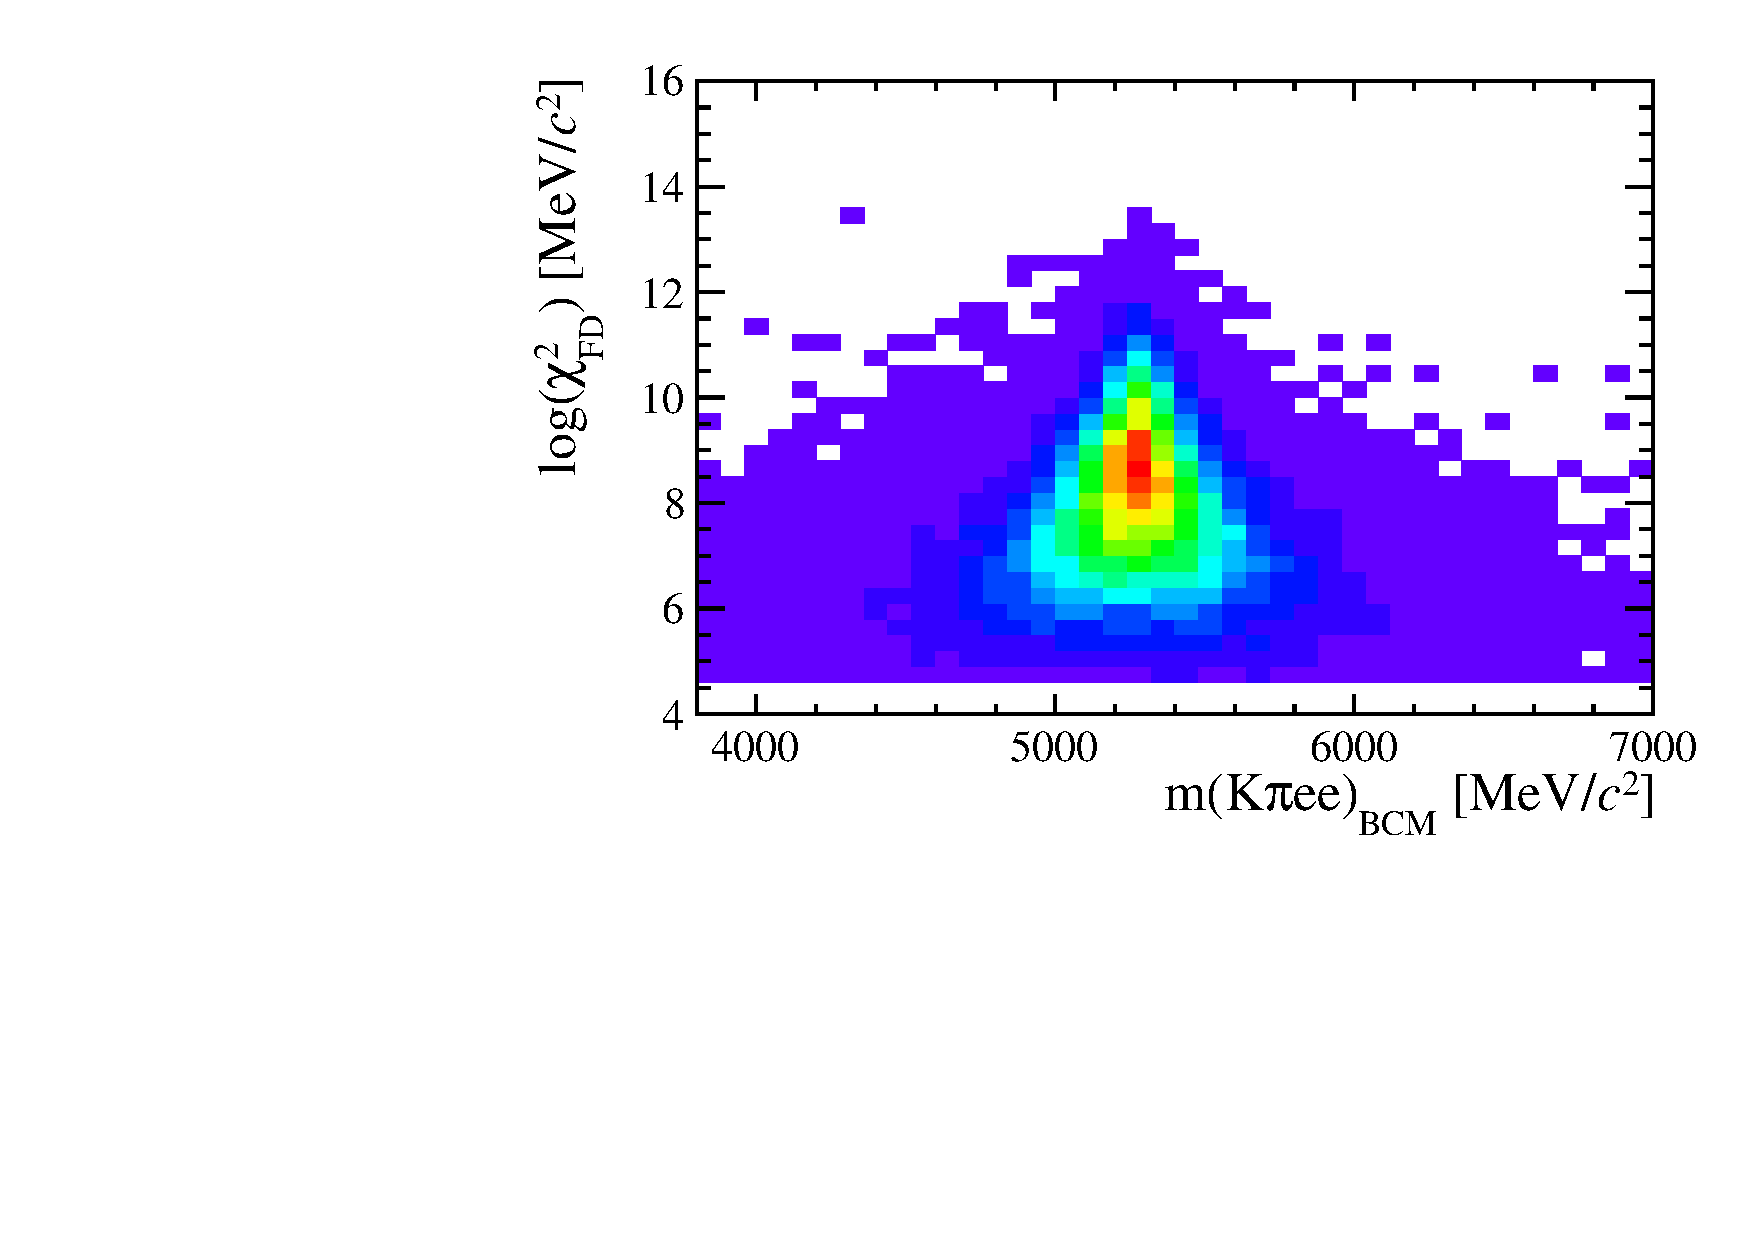
\includegraphics[width=0.48\textwidth]{RKst/figs/HOP/HOP_sig_low.pdf}
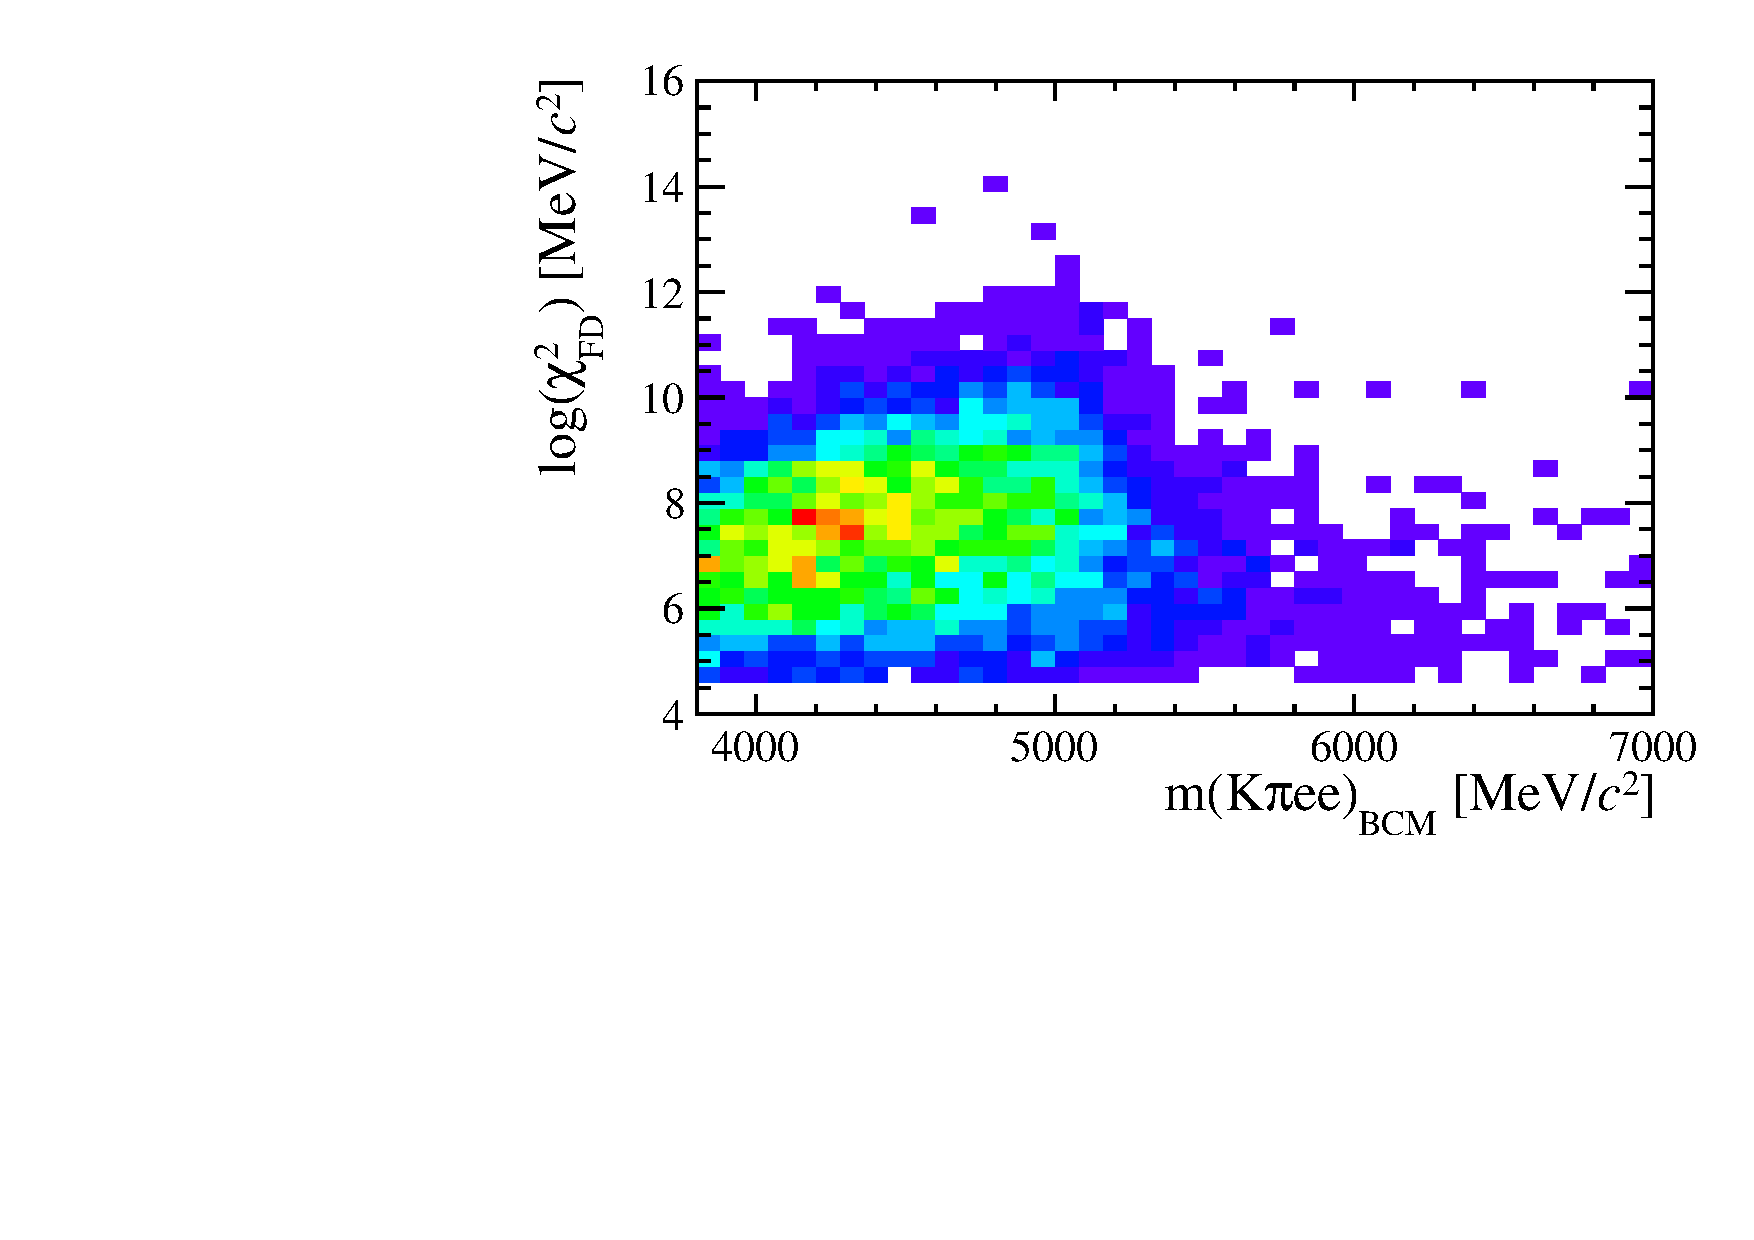
\includegraphics[width=0.48\textwidth]{RKst/figs/HOP/HOP_bkg_low.pdf}
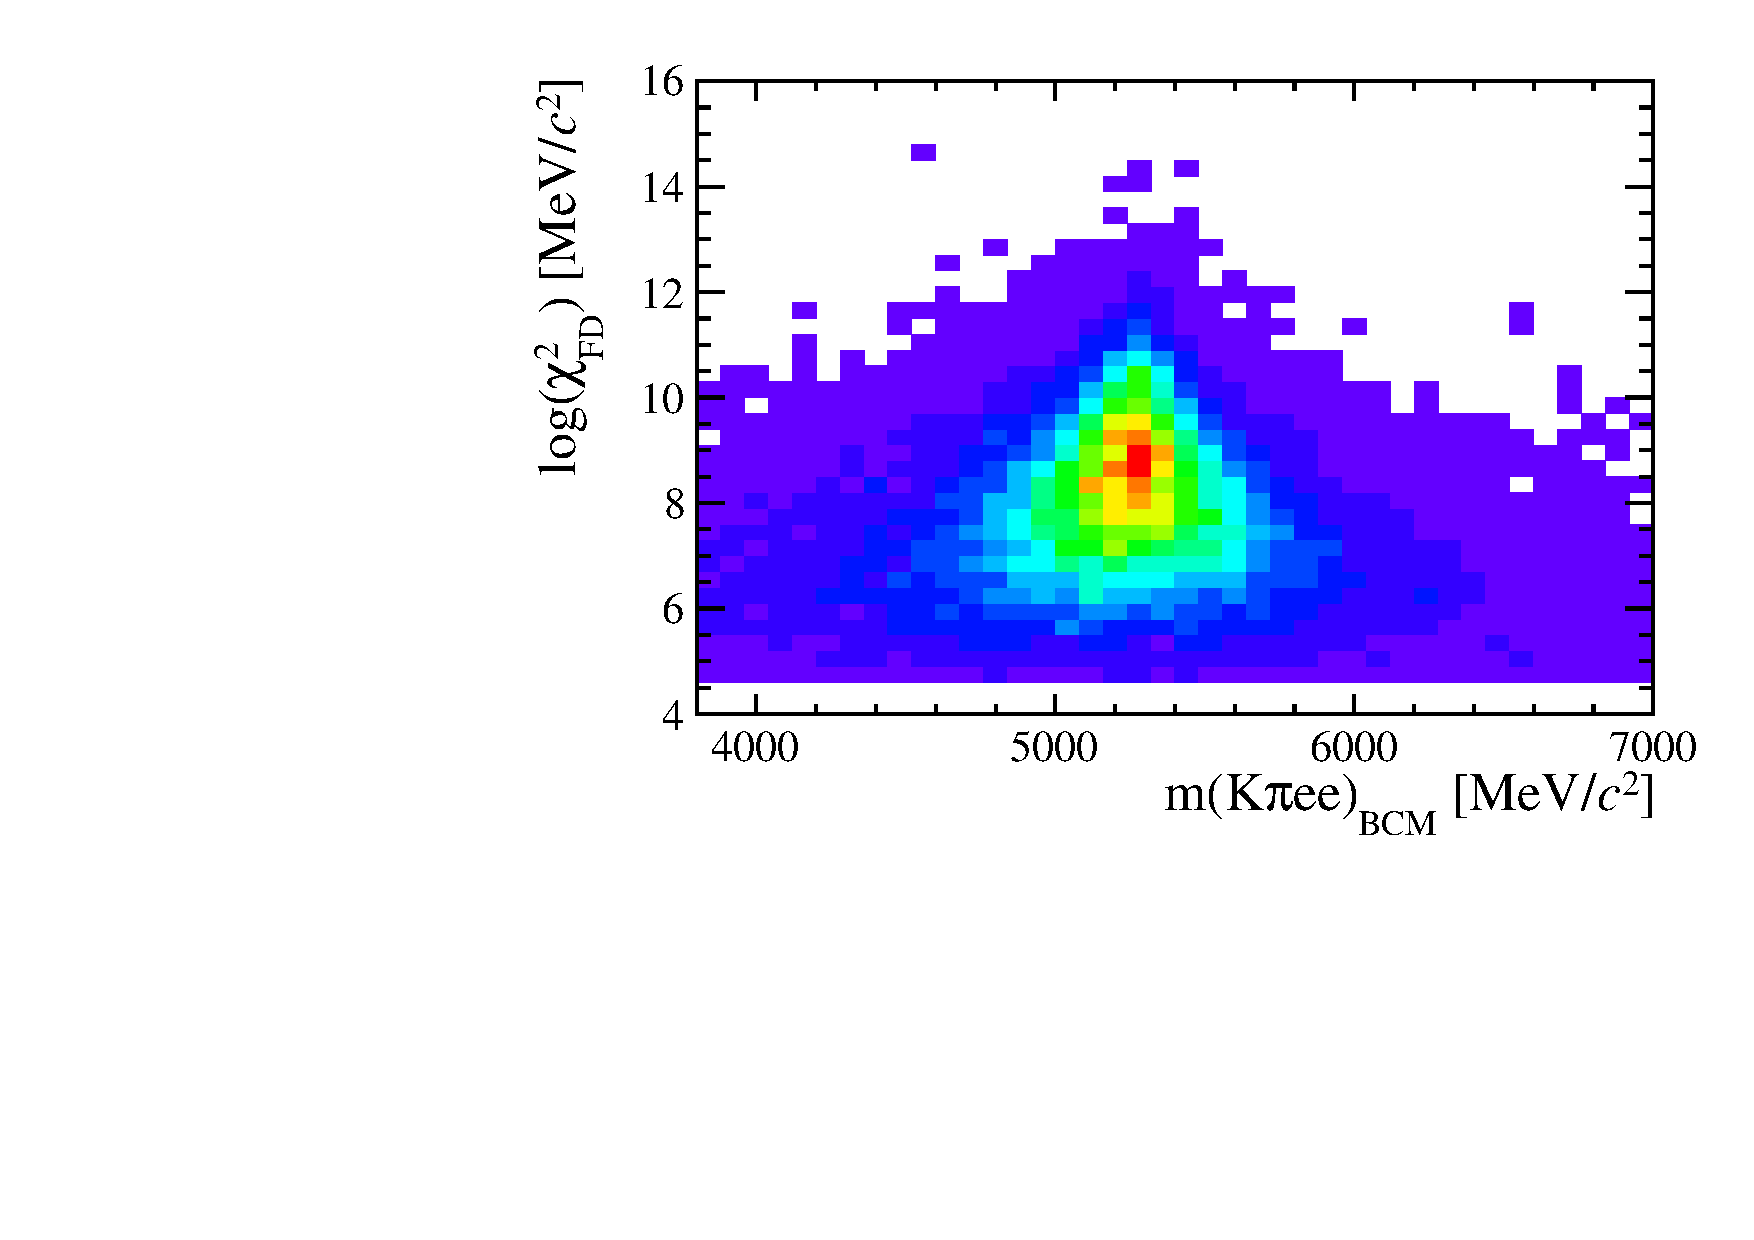
\includegraphics[width=0.48\textwidth]{RKst/figs/HOP/HOP_sig_central.pdf}
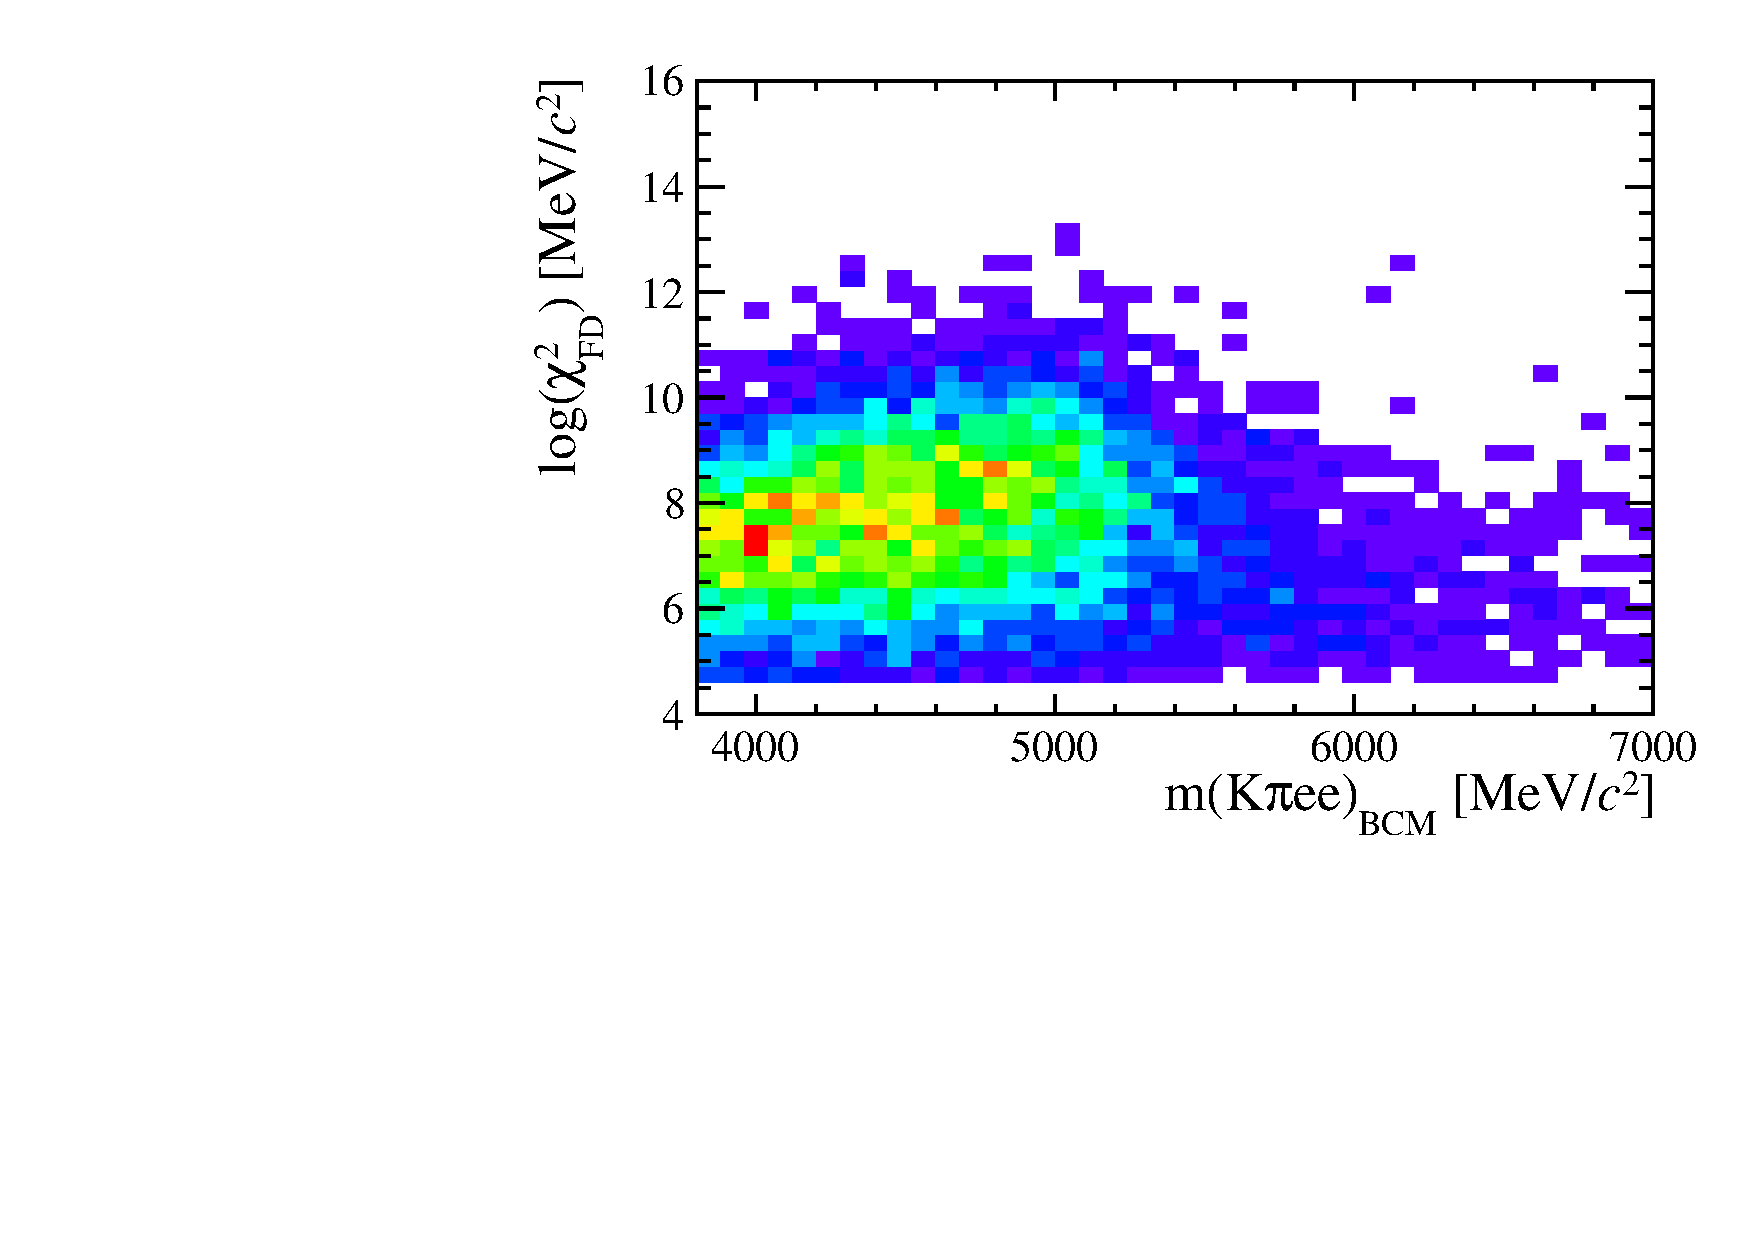
\includegraphics[width=0.48\textwidth]{RKst/figs/HOP/HOP_bkg_central.pdf}
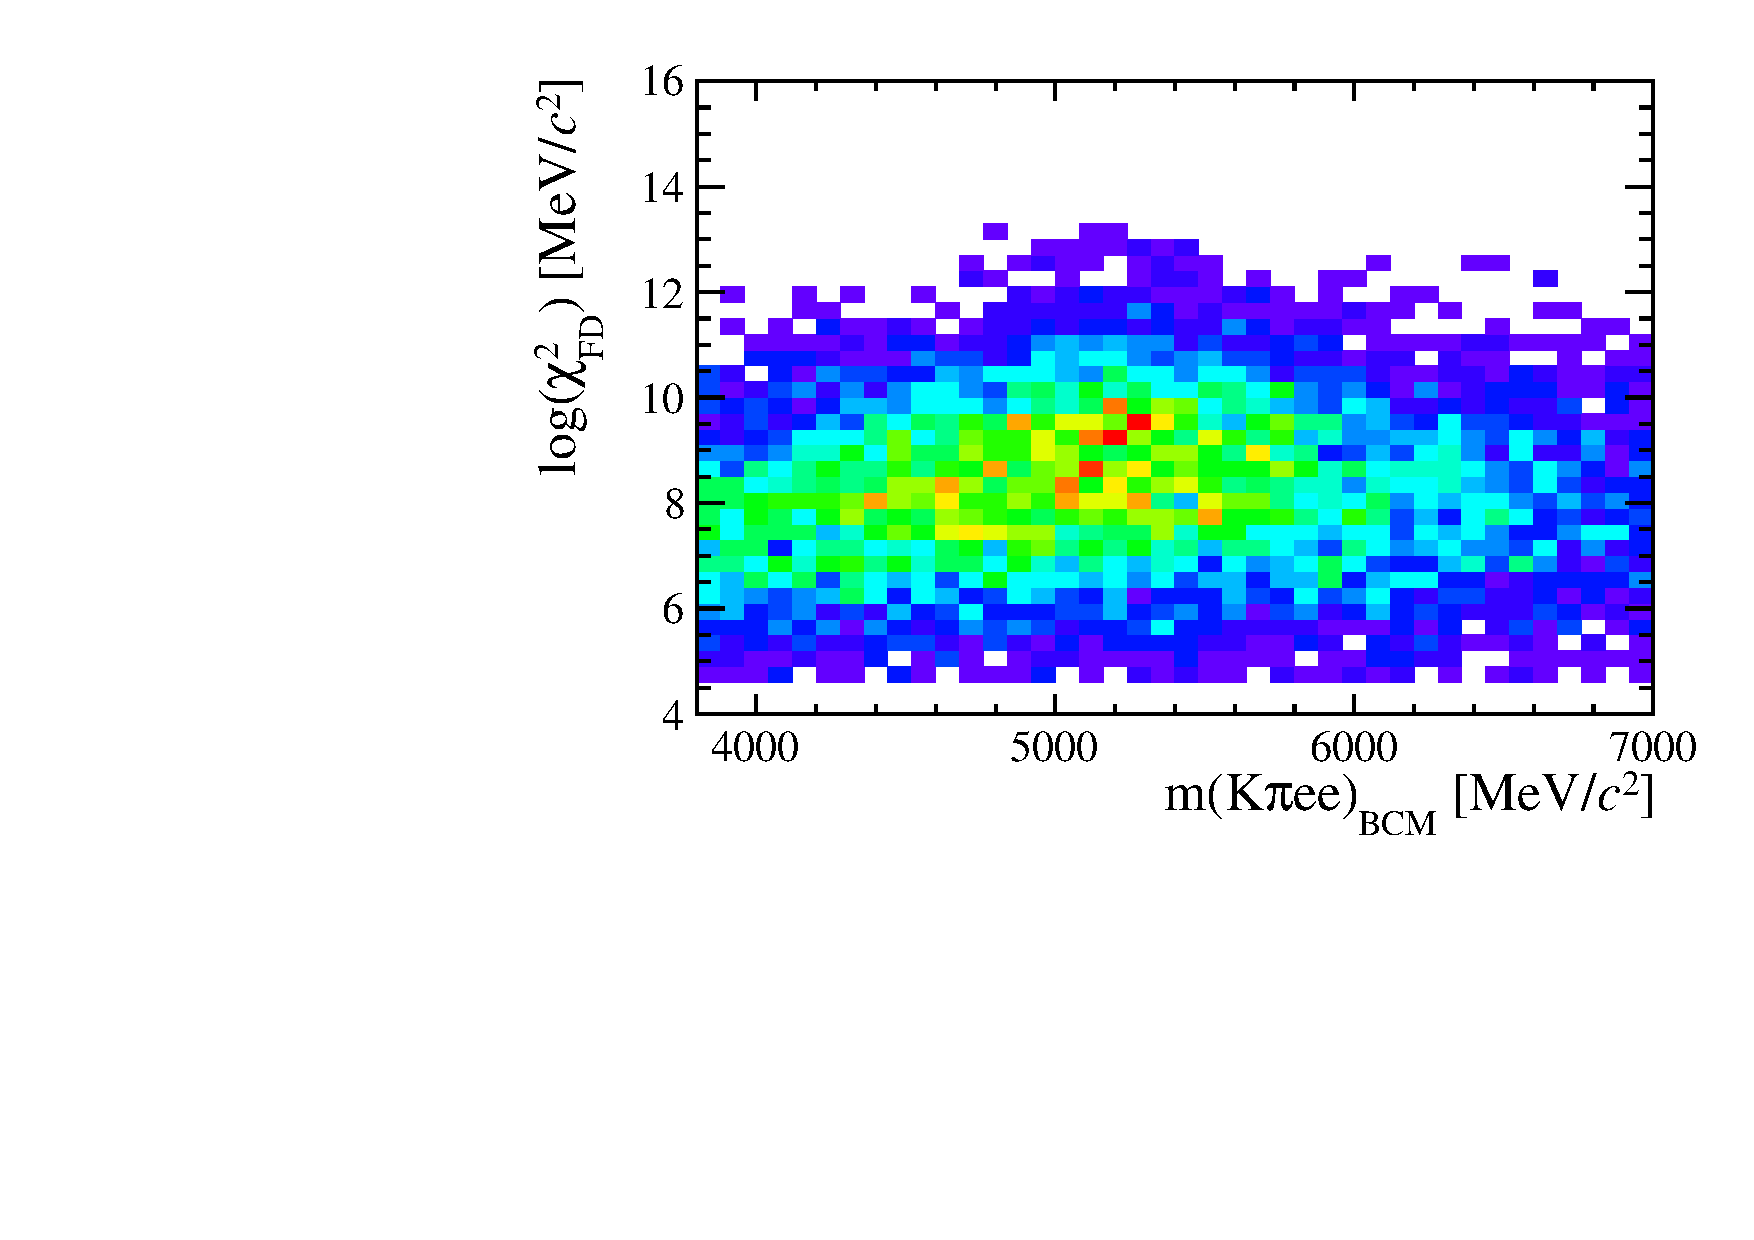
\includegraphics[width=0.48\textwidth]{RKst/figs/HOP/HOP_sig_high.pdf}
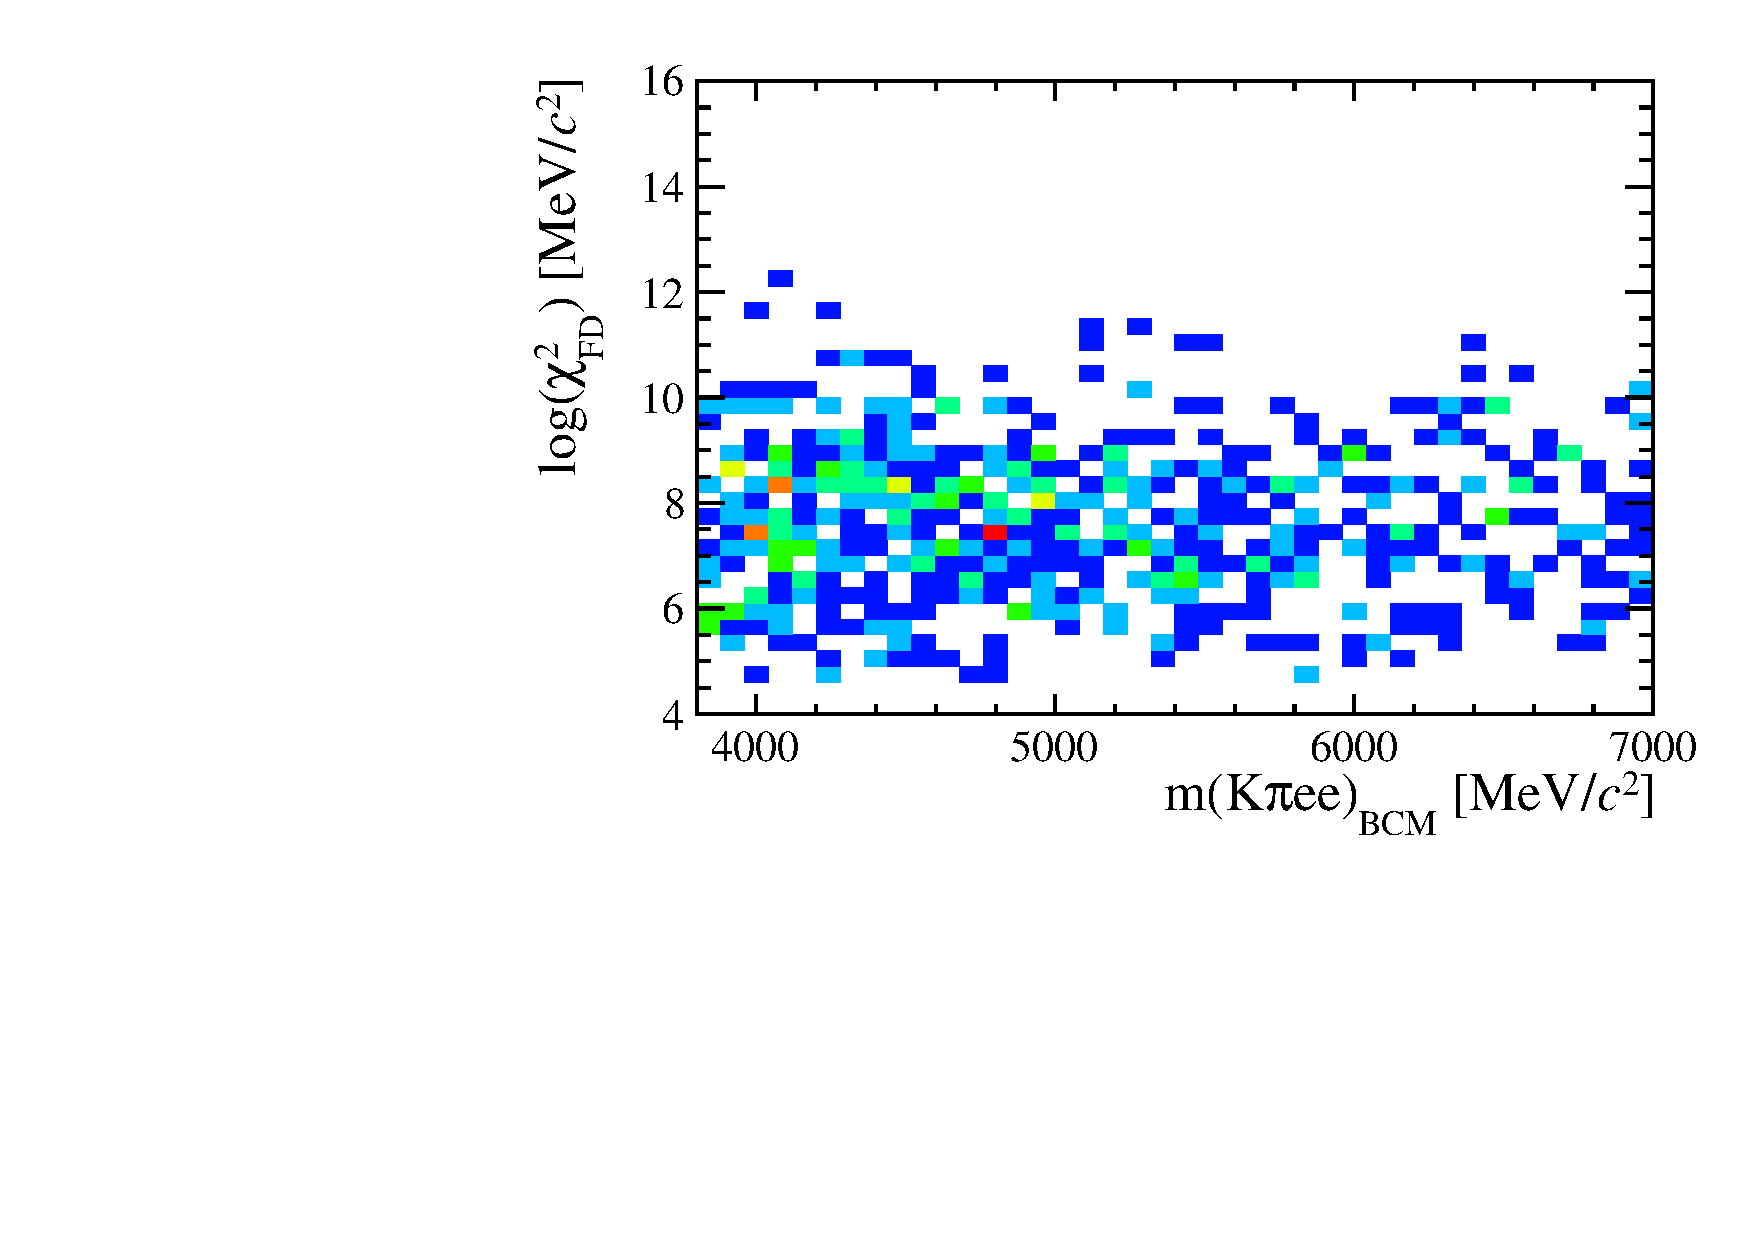
\includegraphics[width=0.48\textwidth]{RKst/figs/HOP/HOP_bkg_high.pdf}
\caption{Two-dimensional distribution of $\chi^2_{\rm FD}$ \vs \mbcm for (left) \BdToKstee signal and (right) partially-reconstructed background.
From top to bottom the low-, central- and high-\qsq intervals.}
\label{fig:hop}

%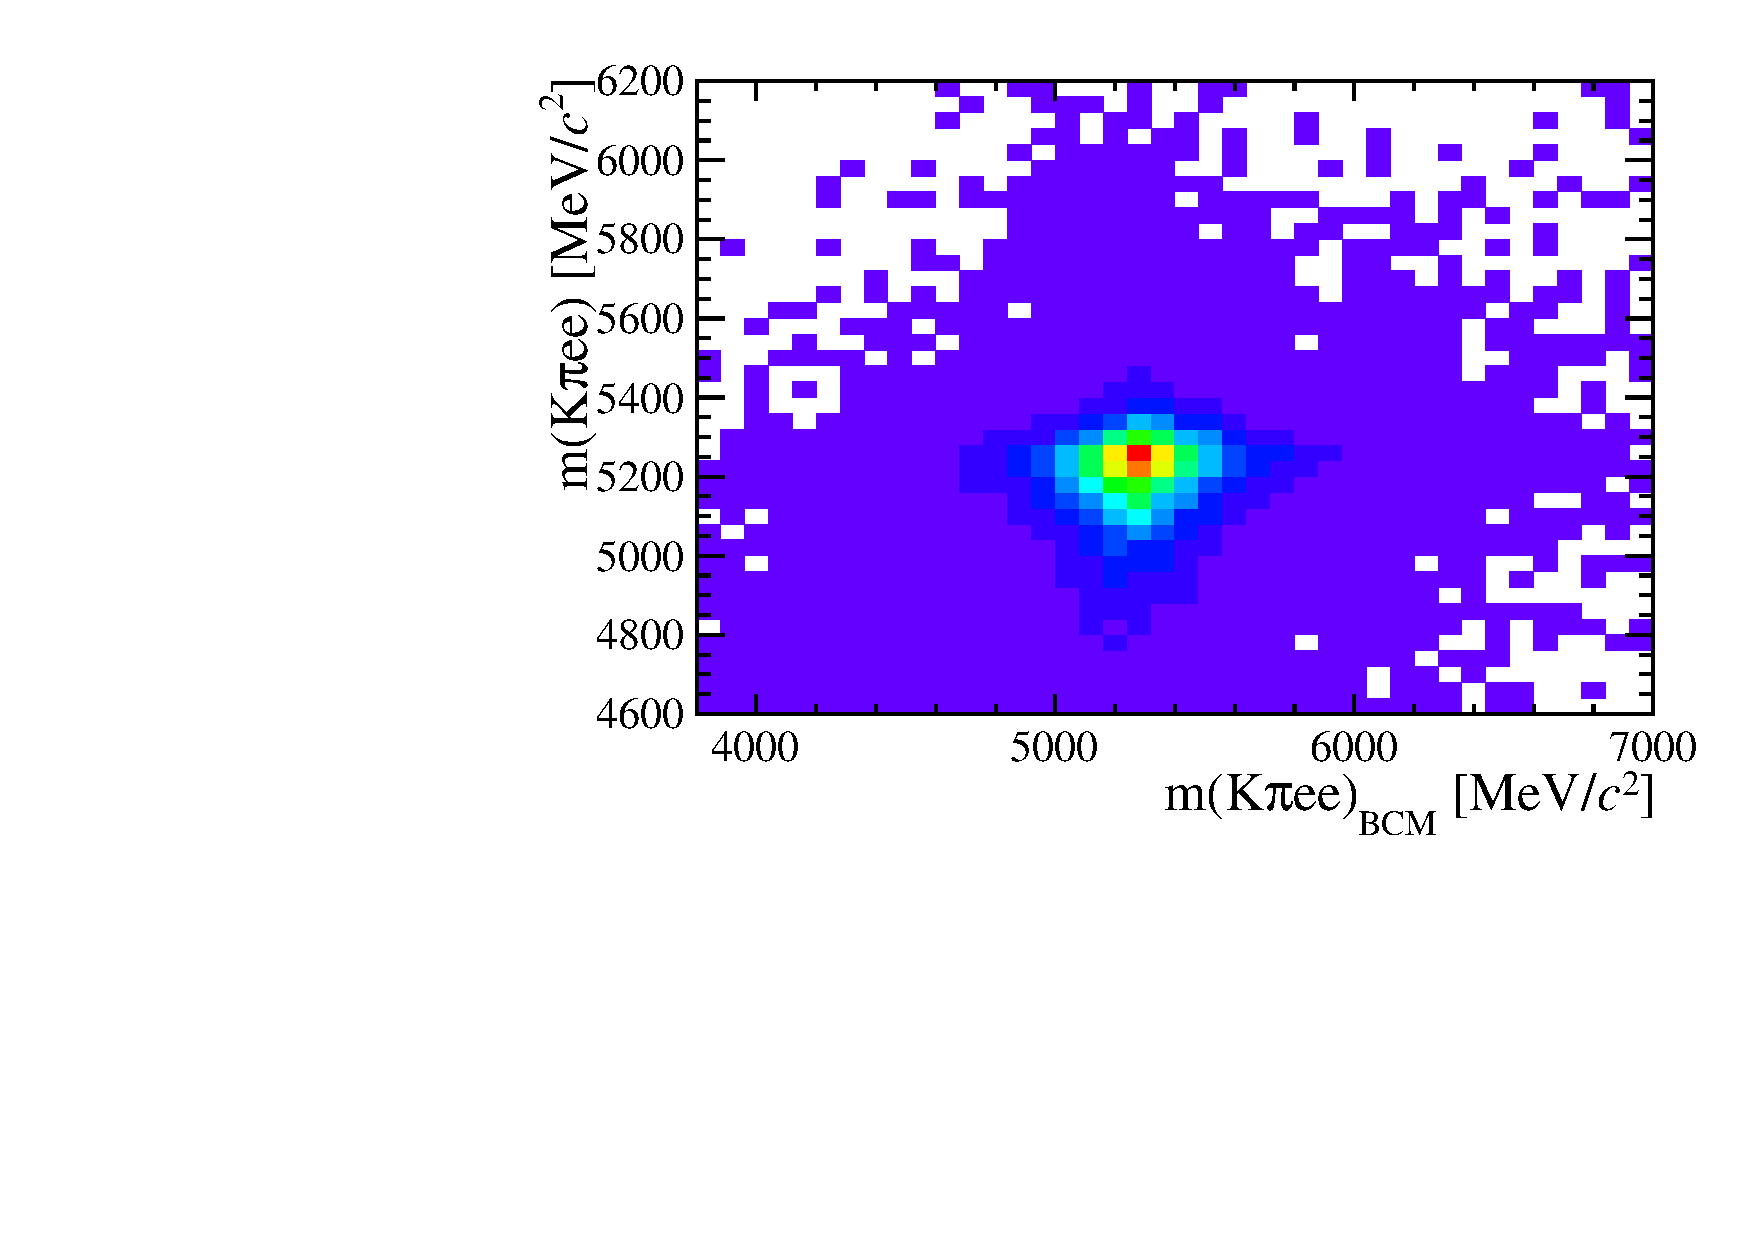
\includegraphics[width=0.48\textwidth]{RKst/figs/HOP/HOPvsM_sig_low.pdf}
%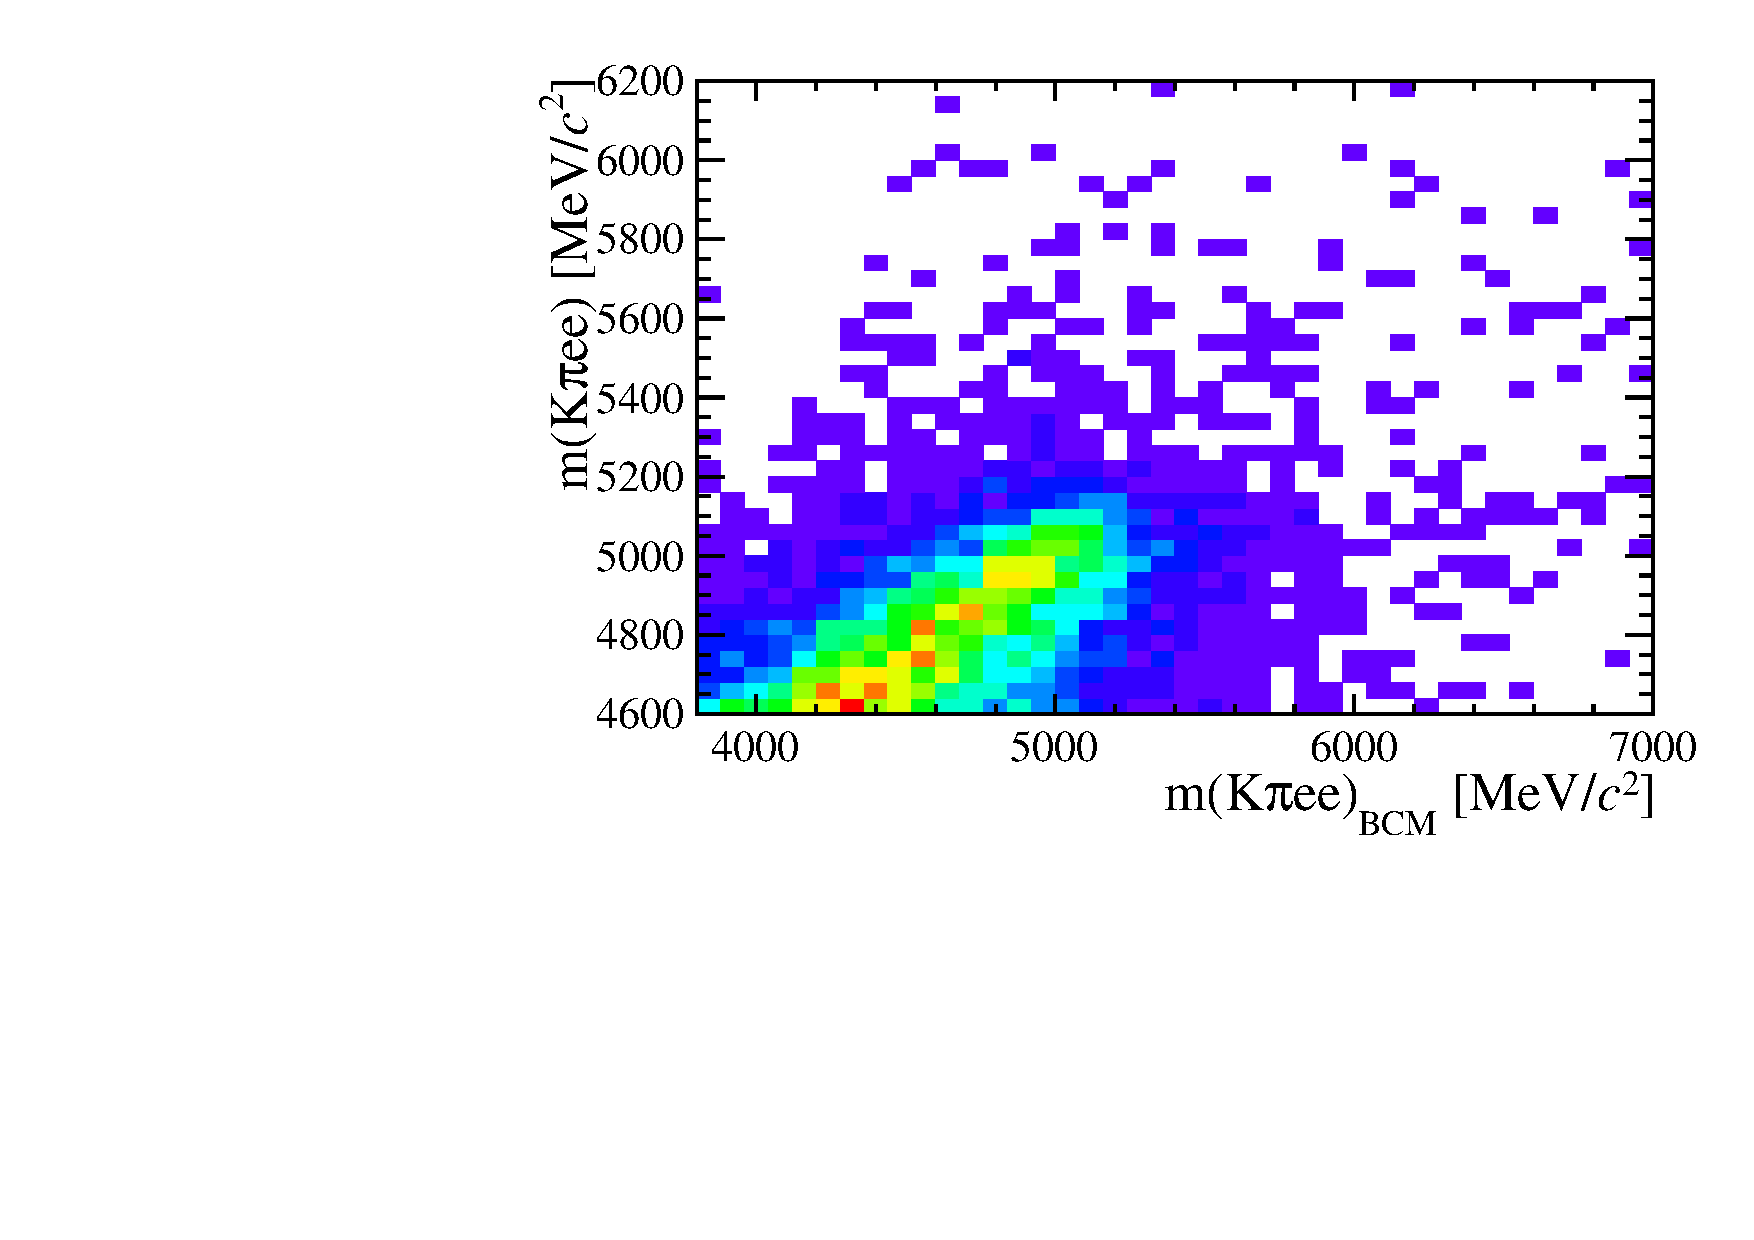
\includegraphics[width=0.48\textwidth]{RKst/figs/HOP/HOPvsM_bkg_low.pdf}
%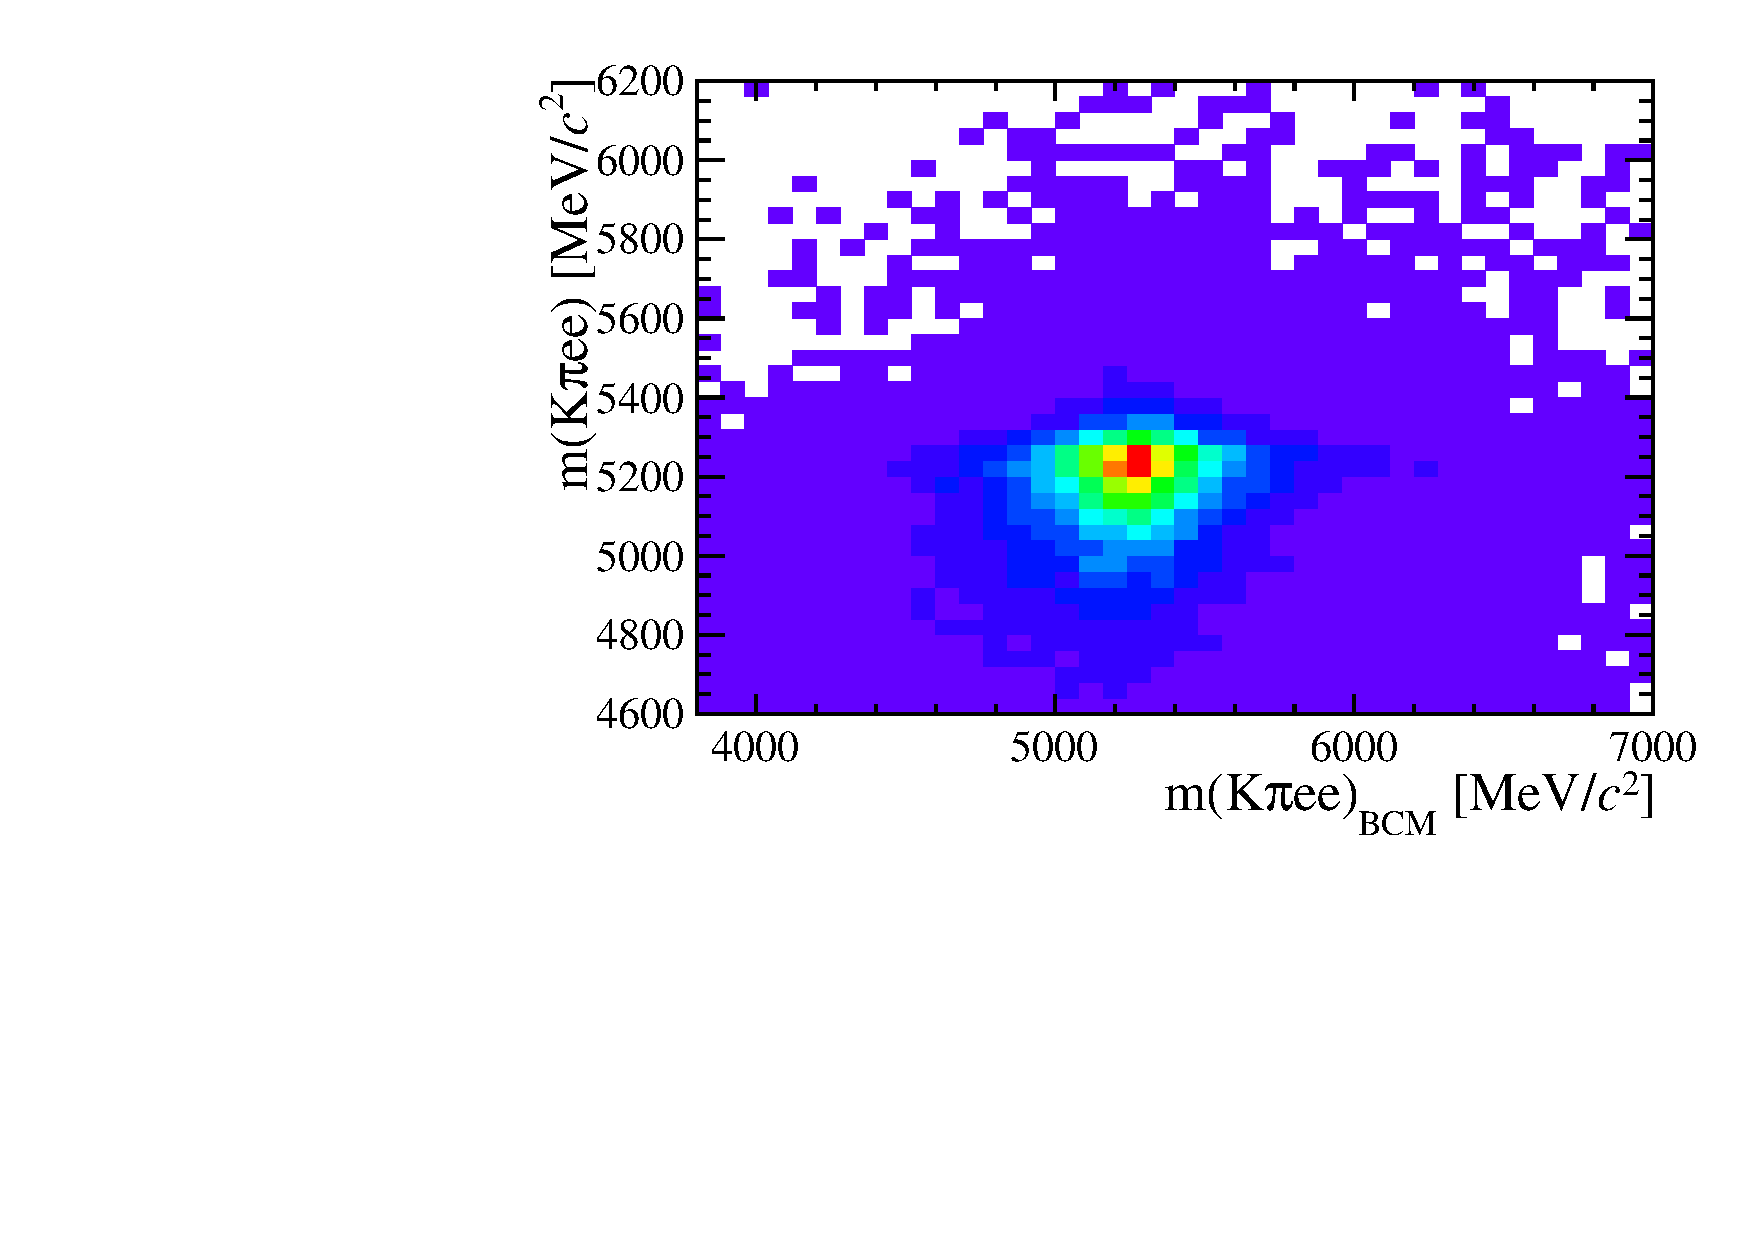
\includegraphics[width=0.48\textwidth]{RKst/figs/HOP/HOPvsM_sig_central.pdf}
%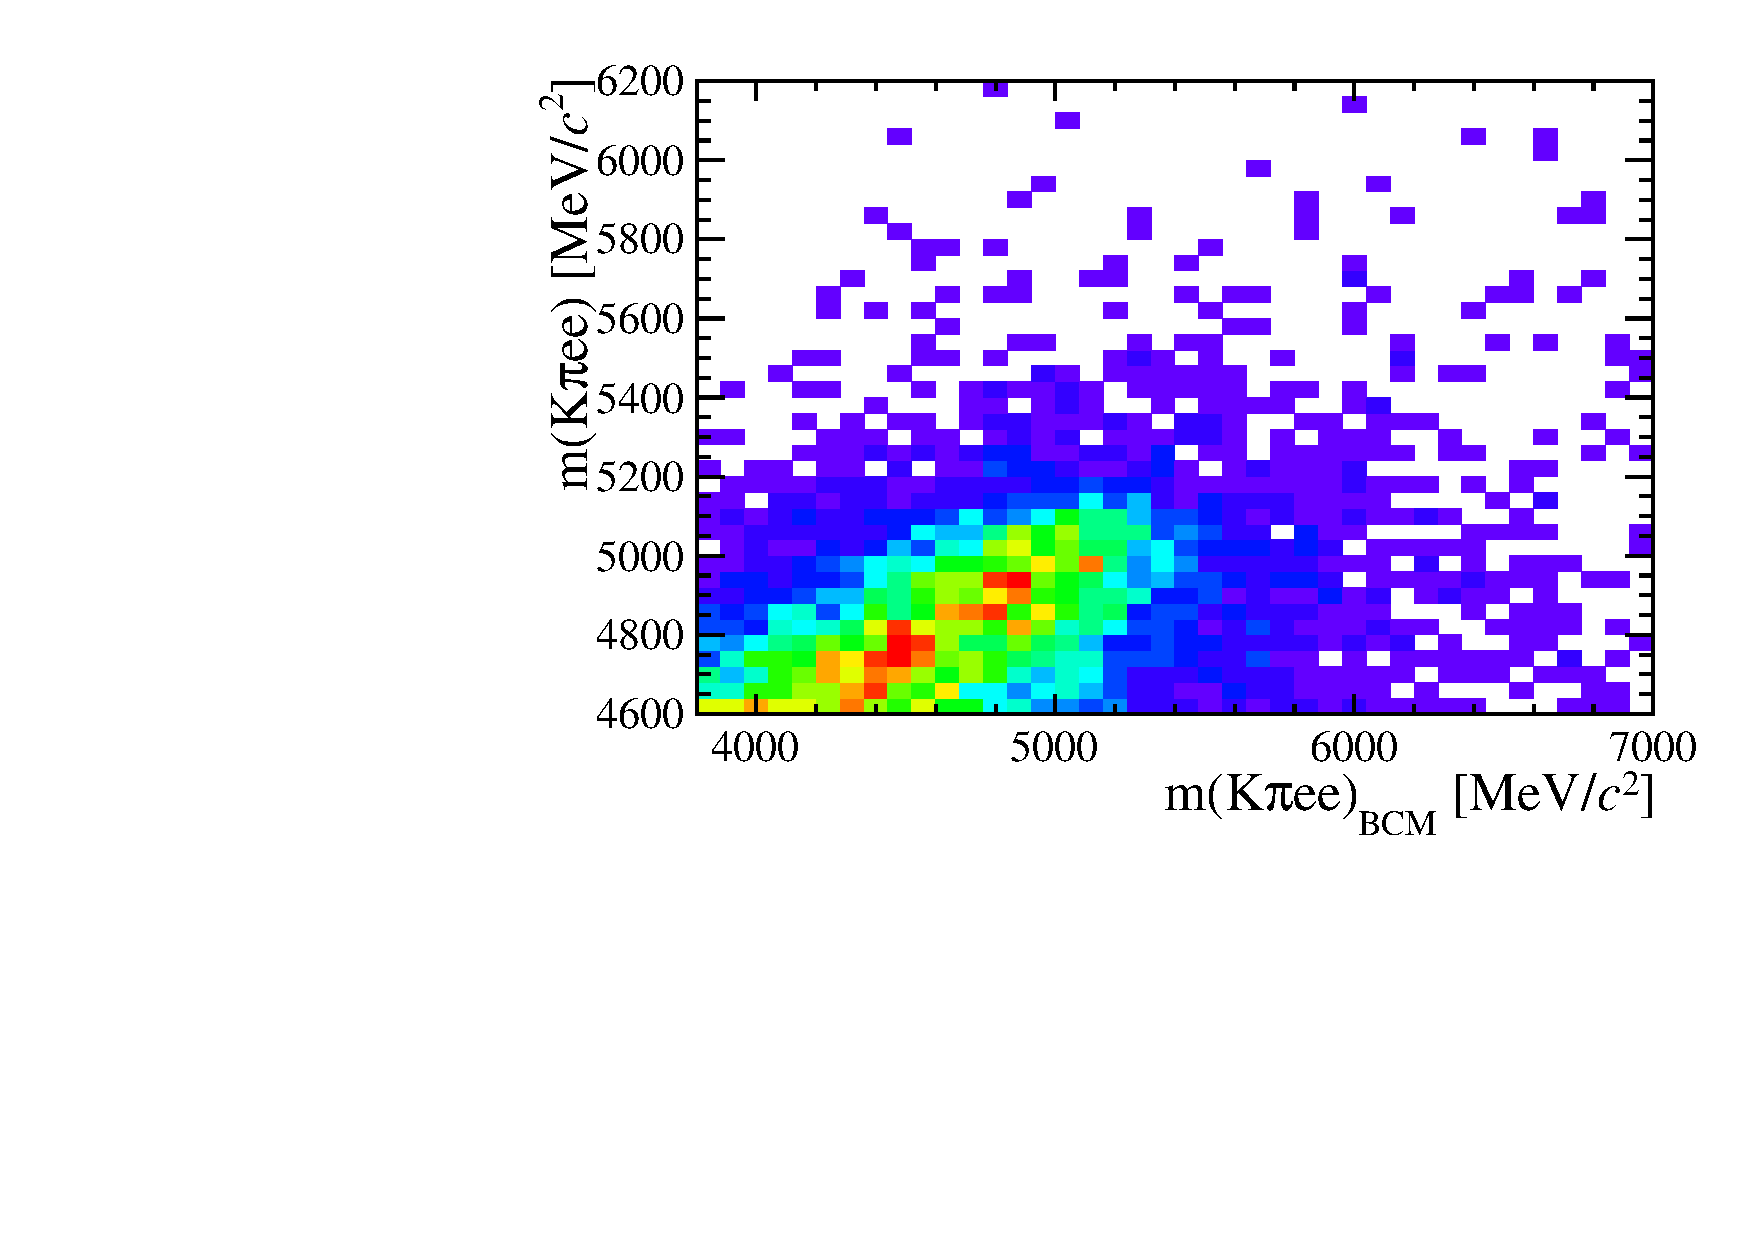
\includegraphics[width=0.48\textwidth]{RKst/figs/HOP/HOPvsM_bkg_central.pdf}
%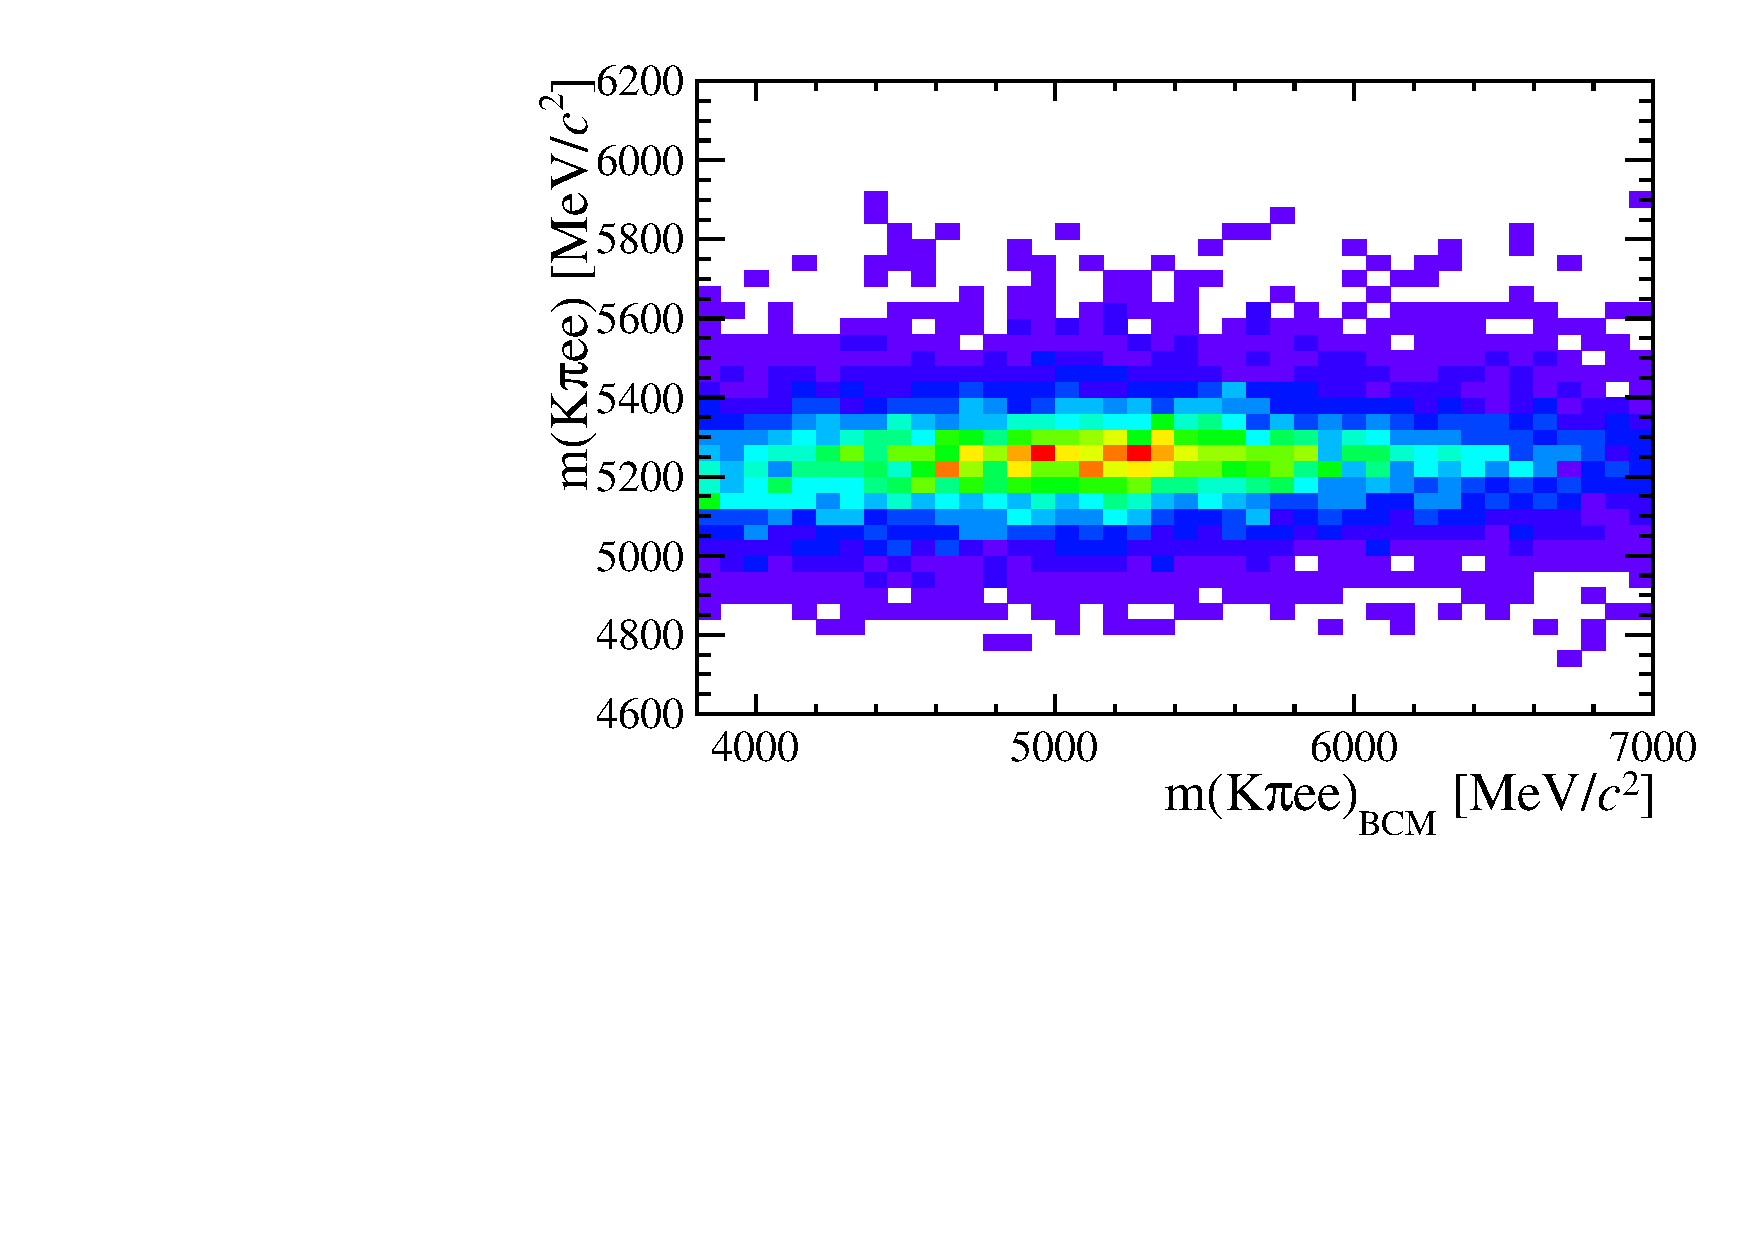
\includegraphics[width=0.48\textwidth]{RKst/figs/HOP/HOPvsM_sig_high.pdf}
%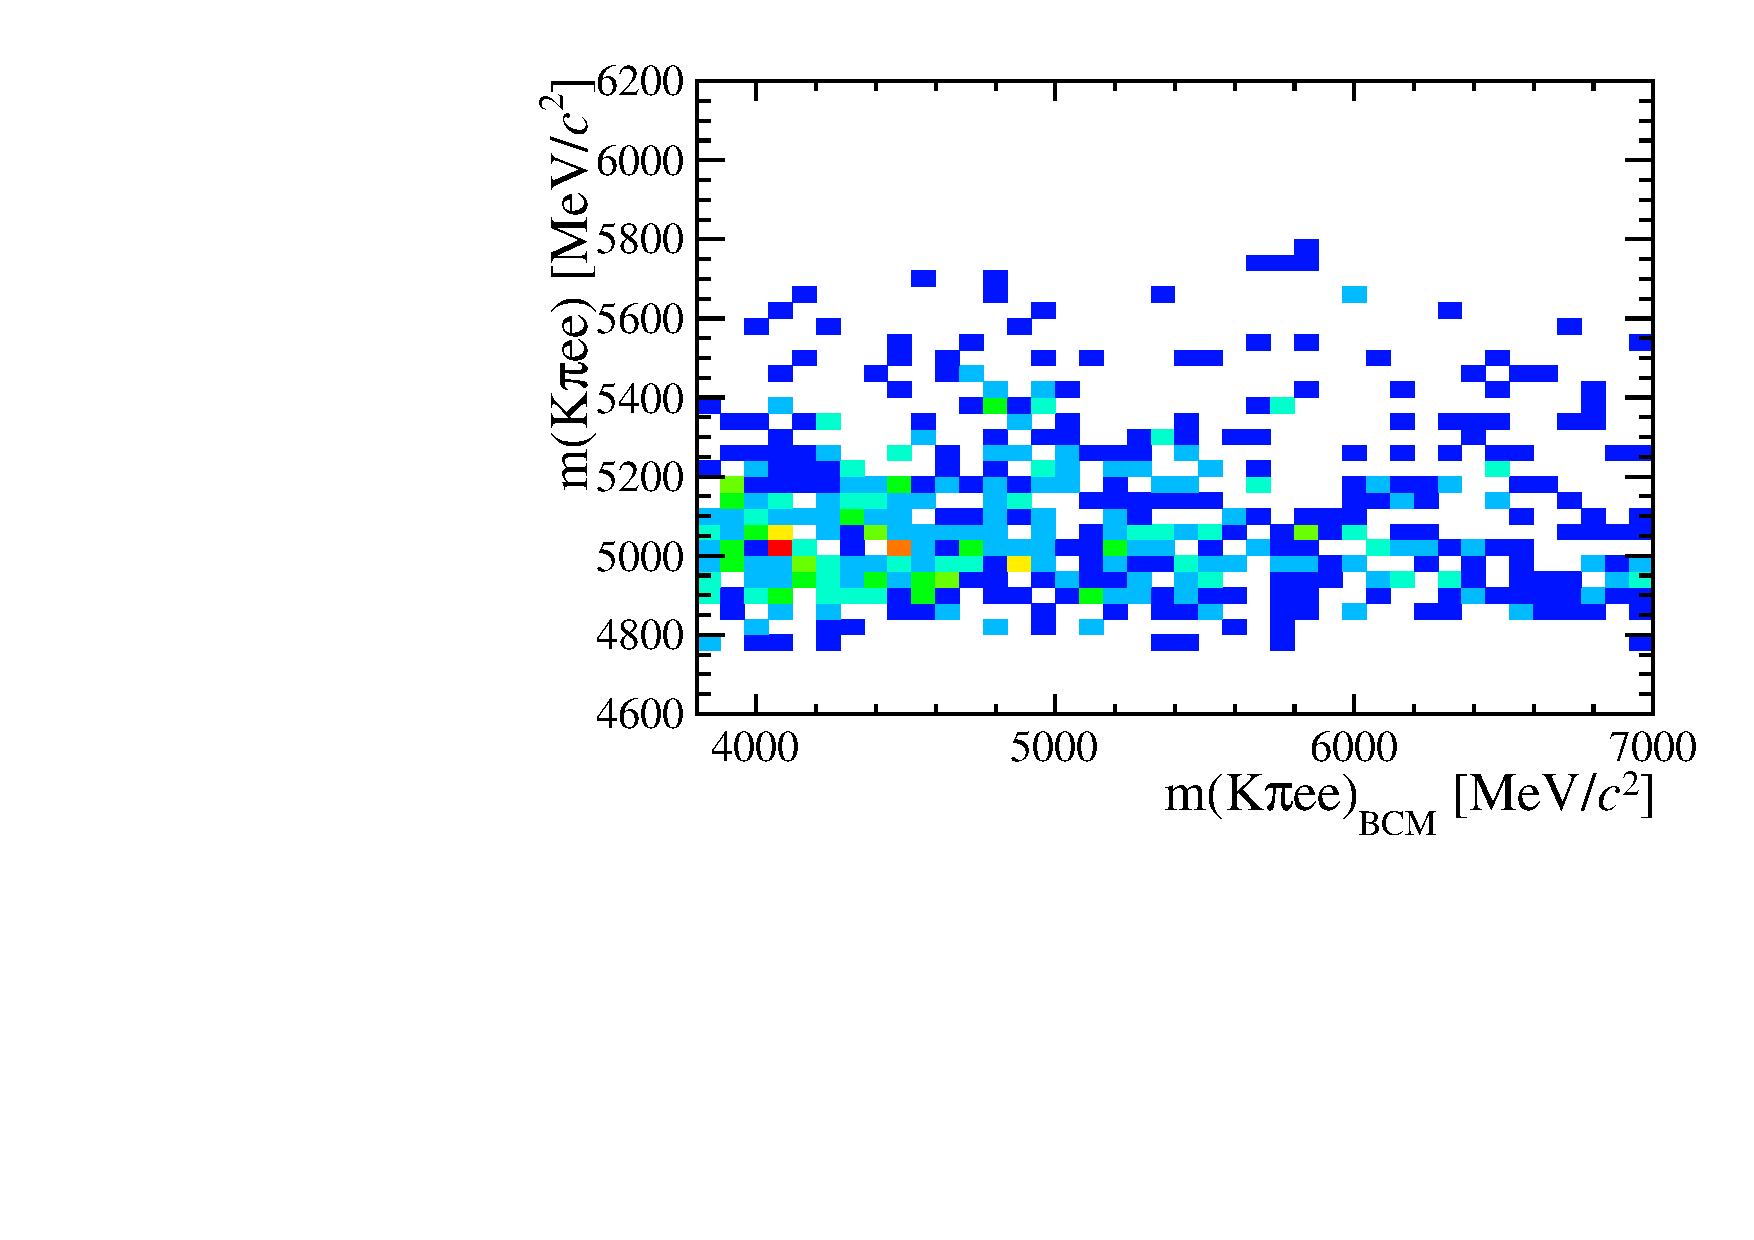
\includegraphics[width=0.48\textwidth]{RKst/figs/HOP/HOPvsM_bkg_high.pdf}
%\caption{Two-dimensional distribution of $m(K\pi ee) \vs \mbcm for (left) \BdToKstee signal and (right) partially-reconstructed background.
%From top to bottom the low-, central- and high-\qsq intervals.}
%\label{fig:hop2}
\end{figure}


\subsection{Multivariate analysis}
\label{sec:RKst_mva}

The final selection is performed using a neural network classifier based on the \mbox{\textsc{NeuroBayes}}
package~\cite{Feindt:2006pm,feindt-2004}. The multivariate analysis is intended to remove
some combinatorial background and obtain a clearer signal peak. In order to avoid biases, a so-called $k$-fold
approach is adopted to train and optimise the classifier, using $k=10$. In this method, the samples are divided into 
$k$ equally sized subsamples; $k$ classifiers are then trained and optimised each one using $(k-1)$ of the subsamples 
and applied to the $k$th one. This approach ensures that a classifier is never applied to the candidates used for its training.
Each classifier is trained on half of the candidates included in the $(k-1)$ samples and optimised using the other half,
which ensures that candidates used for training are not used for optimisation.

{\bf Samples:}

Representative samples of the signal and background are needed to train the classifier.
For the signal, fully reconstructed \BdToKstmm and \BdKstee simulated events can be used.
%The simulation is corrected improve the data-simulation agreement as described in (see Sec. \ref{sec:RKst_mc_weighting}).
Instead a sample representative of the background can be obtained using real data candidates
in the upper \Bz sideband: $m(K\pi\mu\mu) > 5400$~\mevcc~ and $m(K\pi ee) > 5600$~\mevcc.
The lower sideband is not used in the training as it contains a significant fraction of misreconstructed background.
All pre-selection requirements are applied to the background samples used for the training.
As L0 and PID variables are not well described in simulation these cuts are not applied to the simulation
but their effect is taken into account by event weights.
%To train the classifier 50\% of the sideband events was used, keeping the other 50\% for testing.
An approximately equal number of signal and background candidates is used for the training
which corresponds to about $10^3$ electron and $10^4$ muon candidates.
%, which
%is driven by the amount of background available.

{\bf Training:}

The neural network input consists of 24 variables carrying information about the kinematics of the decays
and the quality of tracks and vertices. All the variables used are listed in Tab.~\ref{tab:RKst_mva_vars}.
% and their correlation is graphically represented in Fig.~\ref{fig:Rkst_nnCorrelation}.
%In these figures the variable with ID = 1 is the neural-network output and the other IDs are reported in Tab.~\ref{tab:RKst_mva_vars}.
The single most discriminating variable is $\chisq_{\rm DTF}$, the \chisq of a kinematic fit (see Sec.~\ref{sec:DTF})
that constrains the decay product of the \Bz, the \Kstarz and the dimuon, to originate from their respective vertices.
Other variables that contribute significantly are the \chisqip of \jpsi and \Kstarz, the transverse momentum
of the \Bz and the pointing direction (\verb!DIRA!) of the reconstructed \Bz to the primary vertex.
%
%
\begin{table}
\centering
\caption{List of variables used as inputs for the neural-network training.
%Next to each variable the ID number in brackets provides the index
%reported in the correlation matrices shown in Fig.~\ref{fig:Rkst_nnCorrelation}.
}
\begin{tabular}{$l|^l}
\rowstyle{\bfseries}
Particle 	& Variables \\ \hline
\Bz		& \pt, \quad \chisqip, \quad $\chisq_{\rm FD}$, \quad $\chisq_{vtx}/\text{ndf}$, \quad \texttt{DIRA}, \quad $\chisq_{\rm DTF}/\text{ndf}$ \\
\Kstarz	& \pt, \quad \chisqip, \quad $\chisq_{\rm FD}$, \quad $\chisq_{vtx}/\text{ndf}$, \quad \texttt{DIRA} \\
$h$		& $\mathrm{min},\mathrm{max}(p_{\textrm{T}, \kaon},p_{\textrm{T}, \pi})$, \quad $\mathrm{min},\mathrm{max}(\chi_{\textrm{IP}, \kaon}^{2},\chi_{\textrm{IP}, \pi}^{2})$ \\
$\ell\ell$	& \pt, \quad \chisqip, \quad $\chisq_{\rm FD}$, \quad $\chisq_{vtx}/\text{ndf}$, \quad \texttt{DIRA} \\
$\ell$	& $\mathrm{min},\mathrm{max}(p_{\textrm{T}, \ell^+},p_{\textrm{T}, \ell^-})$, \quad $\mathrm{min},\mathrm{max}(\chi_{\textrm{IP}, \ell^+}^{2},\chi_{\textrm{IP}, \ell^-}^{2})$ \\
%\Bz			& $\chi^2_{\rm DTF}/\text{ndf}$ [1], DIRA [19], $\chi^2_{\rm FD}$ [15], $\chi^2_{vtx}/\text{ndf}$ [12], \chisqip [14], \pt [7] \\
%\Kstar		& $\chi^2_{\rm FD}$ [21], $\chi^2_{vtx}/\text{ndf}$ [11], \chisqip [2], \pt [5] \\
%Dilepton	& $\chi^2_{\rm FD}$ [17], $\chi^2_{vtx}/\text{ndf}$ [13], \chisqip [20], \pt [6] \\
%$e$			& \chisqip [3][4], \pt [9][10]\\
%$\mu$		& \chisqip [14][15], \pt [9][10]\\
%K			& \chisqip [18], \pt [16]\\
%$\pi$		& \chisqip [22], \pt [8]\\
\end{tabular}
\label{tab:RKst_mva_vars}
\end{table}
%
\begin{figure}[b]
\centering
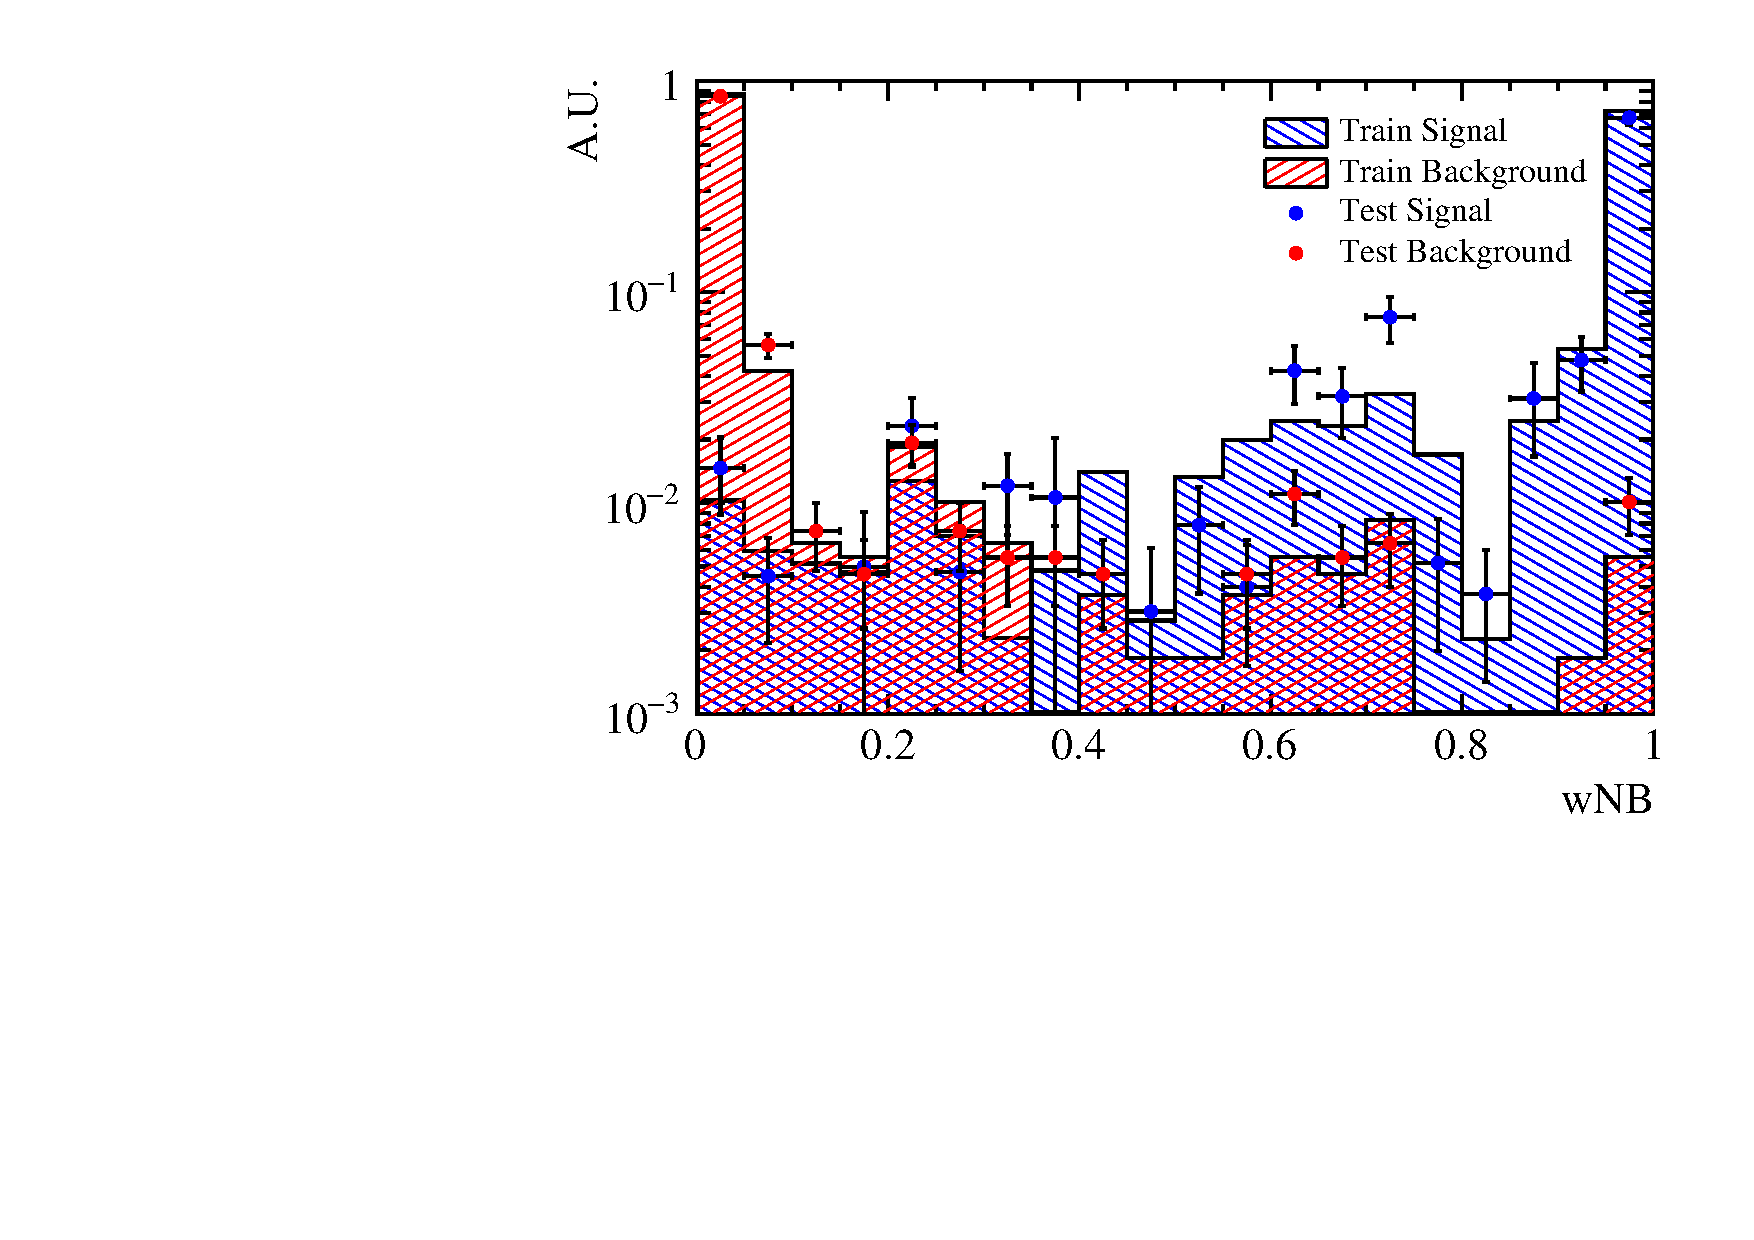
\includegraphics[width=0.49\textwidth]{RKst/figs/Training/EE_wNB_TrainAndTest.pdf}
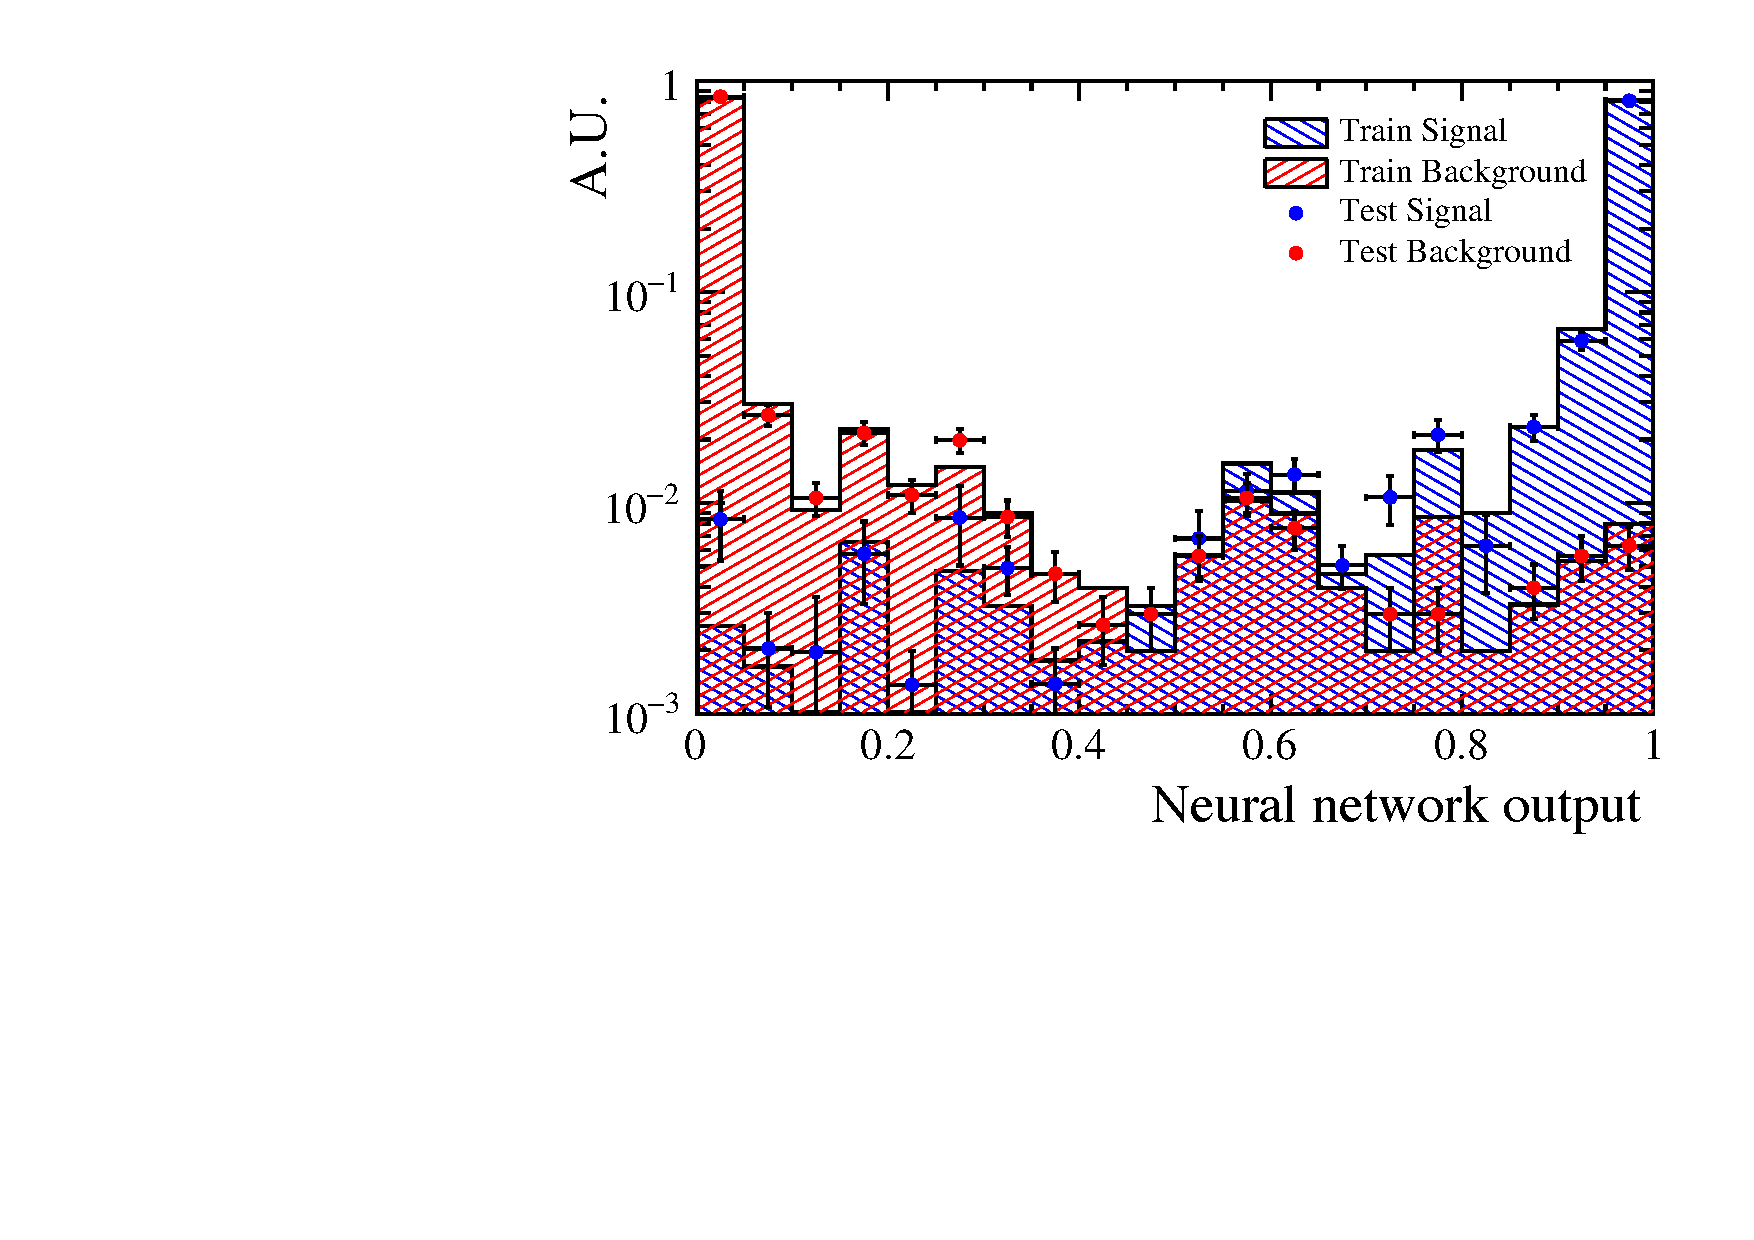
\includegraphics[width=0.49\textwidth]{RKst/figs/Training/MM_wNB_TrainAndTest.pdf}
\caption{Neural network output distributions for training (solid) and test (stripes) samples, for simulated 
signal (blue) and data sideband (red) candidates. For the electron (left) and muon (right) training.}
\label{fig:RKst_nnDist}
\end{figure}
%
%The list the 5 most important variables is reported in Tab.~\ref{tab:RKst_nnInputs}, together
%with information on the relative importance of each input. The meaning of the column headings
%in this table was already explained in Sec.~\ref{sec:Lb_mva}.

%\begin{table}
%\centering
%\caption{Summary of inputs to the neural network in order of importance. The 5 most discriminating variables are shown.
%Column ``adds'' gives correlation significance added by given input when adding it to list of those
%ranked above, ``only this'' provides power of given input alone and ``loss'' shows how much information
%is lost when removing only given input. Decay Tree Fit is performed using DecayTreeFitter tool
%on whole decay chain with constraining tracks to appropriate vertex topology and the $m(p\pi)$
%invariant mass to the PDG value.}
%\begin{tabular}{c|ccc|c|ccc}
%\multicolumn{4}{c|}{Muons} 														& \multicolumn{4}{c}{Electrons}				%		  \\ \hline   
%Input                   			& Adds 			& Only this 	& Loss 			& Input        							& Adds      & Only this & Loss    \\ \hline
%$ \Bz$ $\chi^2_{\rm DTF}/\text{ndf} $		& 80.44 		& 80.44 		& 13.14  		&	$ \Bz$ $\chi^2_{\rm DTF}/\text{ndf} $		& 28.70 		& 28.70 		& 3.94  \\
%$ \Kstar$ $\chisqip $		& 22.26 		& 67.58 		& 3.48  		&	$ \Kstar$ $\chisqip $		& 12.71 		& 25.11 		& 1.57  \\
%$ \Bz\text{DIRA} $		& 10.58 		& 71.24 		& 3.95  		&	$ e_{2}$ $\chisqip $		& 6.56 		& 20.19 		& 3.30  \\
%$ \Kstar$ $\pt $		& 9.16 		& 49.13 		& 2.07  		&	$ e_{1}$ $\chisqip $		& 5.54 		& 19.66 		& 2.60  \\
%$ \jpsi$ $\chisqip $		& 6.58 		& 56.15 		& 1.35  		&	$ \Kstar$ $\pt $		& 3.74 		& 15.35 		& 3.14  \\
%$ \Bz$ $\pt $		& 6.00 		& 41.42 		& 4.39  		&	$ \jpsi$ $\pt $		& 4.81 		& 5.55 		& 3.18  \\
%$ \mu_{1}$ $\pt $		& 2.96 		& 15.85 		& 3.79  		&	$ \Bz$ $\pt $		& 2.78 		& 13.01 		& 2.20  \\
%$ \mu_{2}$ $\pt $		& 2.73 		& 15.04 		& 3.46  		&	$ \pi$ $\pt $		& 3.08 		& 7.93 		& 1.83  \\
%$ \jpsi$ $\pt $		& 3.06 		& 16.41 		& 2.84  		&	$ e_{2}$ $\pt $		& 2.35 		& 9.81 		& 2.74  \\
%$ \Kstar$ $\chi^2_{vtx}/\text{ndf} $		& 2.41 		& 28.14 		& 2.38  		&	$ e_{1}$ $\pt $		& 2.15 		& 8.04 		& 2.28  \\

%$ \Bz$ $\chi^2_{\rm FD} $		& 2.03 		& 63.73 		& 1.37  		&	$ \Kstar$ $\chi^2_{vtx}/\text{ndf} $		& 1.75 		& 7.45 		& 1.89  \\
%$ \mu_{1}$ $\chisqip $		& 1.45 		& 47.90 		& 1.75  		&	$ \Bz$ $\chi^2_{vtx}/\text{ndf} $		& 1.83 		& 27.54 		& 1.95  \\
%$ \mu_{2}$ $\chisqip $		& 1.04 		& 43.24 		& 1.20  		&	$ \jpsi$ $\chi^2_{vtx}/\text{ndf} $		& 1.10 		& 11.28 		& 1.16  \\
%$ K$ $\chisqip $		& 0.84 		& 62.99 		& 0.71  		&	$ \Bz$ $\chisqip $		& 1.11 		& 14.35 		& 1.24  \\
%$ \jpsi$ $\chi^2_{\rm FD} $		& 0.60 		& 55.41 		& 0.62  		&	$ \Bz$ $\chi^2_{\rm FD} $		& 0.93 		& 25.65 		& 1.21  \\
%$ \Bz$ $\chi^2_{vtx}/\text{ndf} $		& 0.56 		& 74.60 		& 0.61  		&	$ K$ $\pt $		& 0.82 		& 14.26 		& 0.61  \\
%$ \pi$ $\pt $		& 0.55 		& 34.94 		& 0.48  		&	$ \jpsi$ $\chi^2_{\rm FD} $		& 0.69 		& 23.85 		& 0.63  \\
%$ \Kstar$ $\chi^2_{\rm FD} $		& 0.34 		& 64.88 		& 0.41  		&	$ K$ $\chisqip $		& 0.56 		& 23.59 		& 0.52  \\
%$ \pi$ $\chisqip $		& 0.32 		& 56.92 		& 0.30  		&	$ \Bz\text{ $		& 0.53 		& 24.50 		& 0.52  \\
%$ \Bz$ $\chisqip $		& 0.30 		& 52.17 		& 0.30  		&	$ \jpsi$ $\chisqip $		& 0.37 		& 23.54 		& 0.38  \\
%$ \jpsi$ $\chi^2_{vtx}/\text{ndf} $		& 0.07 		& 18.35 		& 0.07  		&	$ \Kstar$ $\chi^2_{\rm FD} $		& 0.09 		& 23.66 		& 0.07  \\
%$ K$ $\pt $		& 0.03 		& 43.58 		& 0.03  		&	$ \pi$ $\chisqip $		& 0.01 		& 19.89 		& 0.01  \\
%\end{tabular}
%\label{tab:RKst_nnInputs}
%\end{table}

%\begin{figure}
%\centering
%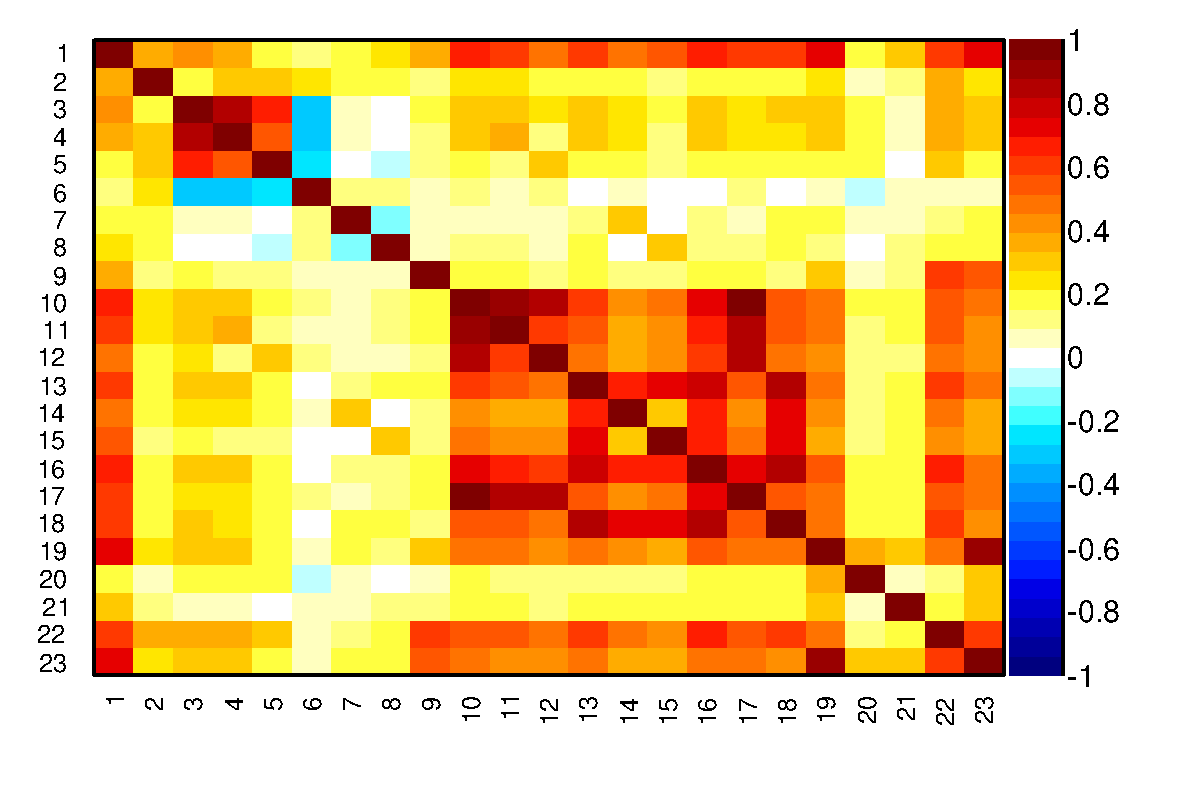
\includegraphics[width=0.8\textwidth]{RKst/figs/Training/electrons/correlation.pdf}
%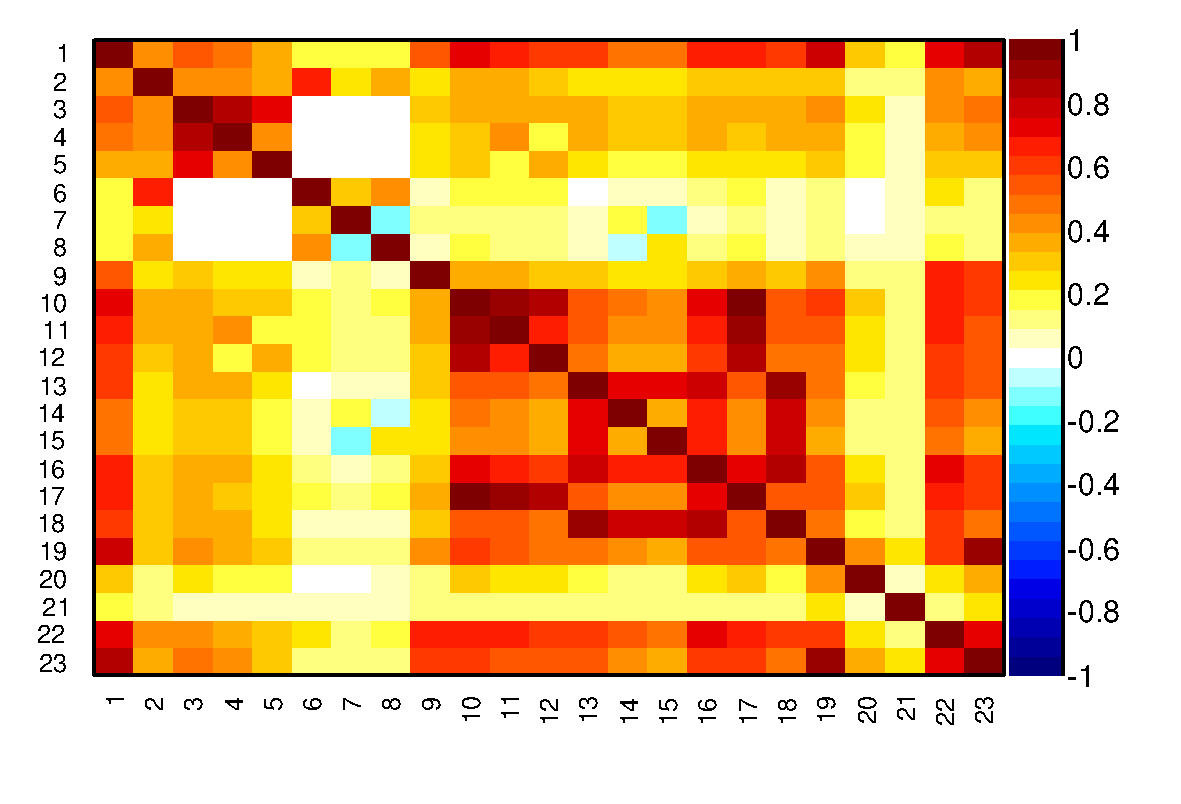
\includegraphics[width=0.8\textwidth]{RKst/figs/Training/muons/correlation.pdf}
%\caption{Graphical representation of correlation matrix between truth and neural network inputs.
%Column/row number 1 is correlation to the truth (whether candidate is signal or background). All
%others give correlation between inputs with numbering scheme corresponding to the id column of
%Tab.~\ref{tab:RKst_nnInputs}. Correlation is calculated using all events without distinguishing signal and
%background.}
%\label{fig:Rkst_nnCorrelation}
%\end{figure}
%

Figure~\ref{fig:RKst_nnDist} shows neural network output distributions for signal and background.
On this plot the distributions from the test samples are also overlaid in order to check for overtraining. 
The distributions follow the same shape but with different fluctuations indicating no
significant overtraining. In general it can be concluded that the neural network is able to separate signal
from background and that the training converged properly.

If too much information is given to the classifier, this can become able to 
calculate the invariant mass of the candidates from its input variables. This could generate fake peaks and it is therefore
important to check for correlations between the 4-body invariant mass and the neural-network output. Figure~\ref{fig:RKst_NNprofiles} 
shows the average neural-network output as a function of the 4-body mass for sideband data and simulated signal candidates.
The distributions are flat showing that no significant correlation is present.


\subsection{Optimisation}
\label{sec:optimisation}

\begin{figure}[t!]
\centering
\includegraphics[width=0.49\textwidth]{RKst/figs/Optimisation/optimizeCut_MM-q2central/fitB_MM_0.pdf}
\includegraphics[width=0.49\textwidth]{RKst/figs/Optimisation/optimizeCut_EE-q2central/fitB_EE_0.pdf}
\caption{Fit to the data sidebands performed to estimate the amount of residual background in the
signal mass window for (left) muons and (right) electrons. The region corresponding to the dashed line is excluded from the fit.}
\label{fig:sideband_fit}
\end{figure}

In order to optimise the requirements on the \mbcm and the neural network output the expected
signal significance, $N_{\mathrm{S}}/\sqrt{N_{\mathrm{S}}+N_{\mathrm{B}}}$, is maximised,
where $N_\mathrm{S}$ ($N_\mathrm{B}$) is the number of rare signal (background) candidates.
When the BCM requirement is applied, the optimisation is performed in a three-dimensional space
($t_{\rm MVA}$, $a_{\rm BCM}$, $b_{\rm BCM}$), where $t_{\rm MVA}$ is the neural-network output threshold below which
a candidate is considered background, and $a_{\rm BCM}$ and $b_{\rm BCM}$ are the parameters of the BCM
cut described in Sec.~\ref{sec:HOP}. Otherwise, only the MVA cut is optimised 
(this is the case for all muons samples and the high-\qsq electron sample).

%The number of signal events accepted for a given neural-network output cut is determined with a data-driven method
%with exploits the resonant channel. First, as an arbitrary number of events can be simulated, this has to be rescaled
%to the expected yield. This is done by fitting \decay{\Bz}{\Kstarz(\jpsi\to\ll)} candidates after pre-selection,
%including all requirements except MVA. The resonant yield is then scaled down by the expected ratio between
%the rare and the resonant channels. The number of background events is instead derived by fitting the combinatorial
%background in the sideband with an exponential function and extrapolating the fit function below the signal peak.

\begin{figure}[h!]
\centering
\includegraphics[width=0.49\textwidth]{RKst/figs/Training/EE_wNB_vs_MPV_bkg.pdf}
\includegraphics[width=0.49\textwidth]{RKst/figs/Training/MM_wNB_vs_MPV_bkg.pdf}
\includegraphics[width=0.49\textwidth]{RKst/figs/Training/EE_wNB_vs_MPV_sgn.pdf}
\includegraphics[width=0.49\textwidth]{RKst/figs/Training/MM_wNB_vs_MPV_sgn.pdf}
\caption{Average value of neural network output as a function of 4-body invariant mass for data
sideband (top) and simulated signal (bottom) candidates for the electron (left) and muon (right) trainings.}
\label{fig:RKst_NNprofiles}
\end{figure}
%
%
\begin{figure}[h!]
\centering
\includegraphics[width=0.49\textwidth]{RKst/figs/Optimisation/optimizeCut_EE-q2central/EE_Optimize_t_MVA.pdf}
\includegraphics[width=0.49\textwidth]{RKst/figs/Optimisation/optimizeCut_MM-q2central/MM_Optimize_t_MVA.pdf}
\includegraphics[width=0.49\textwidth]{RKst/figs/Optimisation/optimizeCut_EE-q2central/EE_ROC_t_MVA.pdf}
\includegraphics[width=0.49\textwidth]{RKst/figs/Optimisation/optimizeCut_MM-q2central/MM_ROC_t_MVA.pdf}
\caption{(top) Dependence of figure-of-merit on the requirement on neural network output.
(bottom) Signal efficiency versus background rejection.
Plots correspond to the electron (left) and muons (right) samples.}
\label{fig:RKst_FOM}
\end{figure}

The number of signal candidates accepted by a given requirement is determined using a data-driven method.
Firstly, \mbox{\BdToKstJPsll} candidates selected with all the requirements except for the MVA, and BCM cuts 
are fitted to determine the total yield. 
% (see Fig.~\ref{fig:RKst_sW_mass}).
This number is then scaled by the ratio between the signal and \mbox{\BdToKstJPsll} branching fractions and
the efficiency ratio: 
%as a function of the cut
%
$$N_{\mathrm{S}} = N_{\jpsi(\ell\ell)} \cdot
\frac{\BR(\mathrm{S})}{\BR(\BdToKstJPsll)} \cdot
\frac{\varepsilon_{\mathrm{S}}}{\varepsilon_{\jpsi(\ell\ell)}} \, .$$

The number of background candidates is also derived from data by fitting the background in the lower and upper 
mass sidebands with an exponential function, and extrapolating the residual yield in the signal region (Fig.~\ref{fig:sideband_fit}).
Because the background shape changes as a function of the requirement that is being optimised, the sidebands are refitted for each considered cut value.
%
%$$N_{\mathrm{B}} \propto N_{\mKpill < 5000 \,||\, \mKpill > 5500} \, .$$

The cut optimisation is performed in a signal mass window of $\pm100~\mevcc$ around the nominal \Bz mass for muons, and between 5000 and 5400~\mevcc~ for electrons.
The average result of the $k$ optimisations is taken as the nominal requirement.
%
%
%
The variation of the signal and background efficiency, signal purity and figure-of-merit as a function of the neural-network output
requirement for the central-\qsq is shown in Fig.~\ref{fig:RKst_FOM}
together with curves of the background rejection as a function of the signal efficiency.
%
%Using the described MVA cuts the signal efficiency is $\sim 95\%$ for the muon channels
%and $\sim 93\%$ for the electron channels (for more details see Sec.~\ref{sec:RKst_efficiency}),
%while the background rejections is $\sim 97\%$ on both samples.
%
After the full selection about $\sim 3\%$ of events still contain multiple candidates
which are removed at random to retain only a single candidate per event.

\clearpage

\subsection{Selection summary}

Table~\ref{tab:sel_summary} summarises the requirements applied for each sample 
on top of the pre-selection requirements described in Sec.~\ref{sec:RKst_trigstripping}.

\begin{table}[ht!]
\begin{center}
\caption{Summary of the selection requirements. The last column
indicates to  which \qsq intervals the requirement is applied.}
\label{tab:sel_summary}
\begin{footnotesize}
\renewcommand\arraystretch{1.4}
\begin{tabular}{c|c|c|c}
\multicolumn{2}{c|}{\textbf{Type}} & \textbf{Requirement} & {\boldmath\qsq} \\
\hline
\multirow{2}{*}{Quality} & \multirow{2}{*}{All tracks}
	& $\chisqndf < 3$ & all \\
	&& {\verb GhostProb } $< 0.4$ & all \\
\hline
ID & \Kstarz & $|m(\kaon\pi) - m_{\Kstarz}^{PDG}| < 100\mevcc$ & all \\
\hline
 \multirow{4}{*}{PID}
	& $K$	& $\texttt{ProbNNk} \cdot (1 - \texttt{ProbNNp}) > 0.05$ & all \\
	& $\pi$	& $\texttt{ProbNNpi} \cdot (1 - \texttt{ProbNNk}) \cdot (1 - \texttt{ProbNNp}) > 0.1$ & all \\
	& $\mu$	& $min(\texttt{ProbNNmu}) > 0.2$ & all $\mu\mu$ \\
	& $e$	& $min(\texttt{ProbNNe}) > 0.2$ & all $ee$ \\
	\hline
	\multirow{19}{*}{BKG}
	& Swap & $|m((\decay{h}{\mu})\mu) - m_{\jpsi, (\psitwos)}^{PDG}| > 60\mevcc$ & all \\
	& \BuToKll & $max(m(K\ell\ell),m((\decay{\pi}{\kaon})\ell\ell)) < 5.1\gevcc$ & all \\
	& \BsToPhill & $m(K(\decay{\pi}{K})) > 1040~\mevcc$ & all \\
	& \decay{\Bd}{\Dm\ep\nu} & $|\cos\theta_\ell\,| < 0.8$ & except high- \\
%	& \BdToKstGee & $\sigma_{Z}(\epem) < 30~\rm{mm}$ & only low- \\
	& \BdToKstG & $\sigma_{z}(\ee) < 30~\rm{mm}$ & except $\gamma(ee)$ \\
\cline{2-4}
	& \multirow{10}{*}{Comb}	& $\texttt{NNout} > 0.68$ & $\mu\mu$ low- \\
	&					& $\texttt{NNout} > 0.64$ & $ee$ low- \\
	& 					& $\texttt{NNout} > 0.85$ & $\mu\mu$ central- \\
	&					& $\texttt{NNout} > 0.97$ & $ee$ central- \\
	& 					& $\texttt{NNout} > 0.40$ & $\mu\mu$ high- \\
	&					& $\texttt{NNout} > 0.93$ & $ee$ high- \\
\cline{3-4}
	& 					& $\texttt{NNout} > 0.06$ & $\jpsi(\mu\mu)$ \\
	&					& $\texttt{NNout} > 0.20$ & $\jpsi(ee)$\\
\cline{3-4}
	&					& $\texttt{NNout} > 0.16$ & $\gamma(ee)$ \\
%	&					& $\texttt{NNout} > 0.36$ & \JPsee \mKpiee \\
	&					& $\texttt{NNout} > 0.68$ & $\psitwos(ee)$ \\
\cline{2-4}
	& Part-reco					& $m(K\pi\ell\ell)_\jpsi	> 5150$~\mevcc		& $\jpsi(ee)$	\\
\cline{2-4}
	& \multirow{3}{*}{Comb, part-reco}	& $\mbcm > 4680 + 31 \cdot \log(\chisq_{\rm FD})$ & $ee$ low- \\
	&							& $\mbcm > 4437 + 64 \cdot \log(\chisq_{\rm FD})$ & $ee$ central- \\
\cline{3-4}	
	&							& $\mbcm > 3380 + 140 \cdot \log(\chisq_{\rm FD})$ & $\gamma(ee)$ \\
%	&							& $\mbcm > 2714 + 164 \cdot \log(\chisq_{\rm FD})$ & $\jpsi(ee)$ \\	
\end{tabular}
\end{footnotesize}
\end{center}
\end{table}




\section{Mass fits}
\label{sec:rkst_fits}

The signal yields are extracted using a simultaneous unbinned maximum likelihood fit
to the 4-body invariant mass, $m(K\pi\ell\ell)$, of the rare and normalisation samples.
The simultaneous fit allows to share parameters e.g. those describing data-simulation differences.
The yields of the rare channels are parameterised as a function of the corresponding \jpsi yields as
%
\begin{equation}
N_{\ell\ell}(r_{\ell\ell}, N_{\jpsi}) = N_{\jpsi} \cdot \varepsilon^{\rm rel} \cdot r_{\ell\ell},
\end{equation}
%
where $\varepsilon^{\rm rel}$ is the relative efficiency between the rare and resonant channels
(given in Tab.~\ref{tab:RKst_RelEff}). Consequently, $r_{\ell\ell}$ corresponds to the efficiency corrected
ratio of the raw rare and resonant yields:
%
\begin{equation}
R_{\ell\ell} = \frac{N_{\ell\ell} / \varepsilon^{\ell\ell}}{N_{\jpsi} / \varepsilon^{\jpsi(\ell\ell)}}.
\end{equation}
%
The two ratios, $R_{ee}$ and $R_{\mu\mu}$, are then used to determine
the $R_{\Kstarz}$ quantity, as described in Sec.~\ref{sec:RKst_result}.
The following subsections contain a description of the line shapes used to model
the signal and background components in each sample.
%The definition of these shapes follows the steps:
%\begin{itemize}
%\item fit simulated signal candidates
%\item fix some parameters in order to obtain shapes which depend on a limited set of parameters
%\item	
%\end{itemize}

\subsection{Muon channels}

For the rare and resonant $\mu\mu$ channels the fitted variable is the $m(K\pi \mu\mu)$ invariant mass coming
from a kinematic fit where all vertices are required to point to their mother particle.
In the resonant case it is beneficial to also constrain the the dimuon mass to the known \jpsi mass.
The effect of the kinematical constraint is to improve the mass resolution by roughly a factor of 2, which results
in a more stable fit. Furthermore, mis-reconstructed background candidates are pushed away from
the \Bz peak, which allows to use a wider mass window to better constrain the combinatorial background slope.
The mass spectrum is fitted in the range 5150--5800~\mevcc~ with the lower limit
chosen to totally exclude partially reconstructed background.
As it is not needed to model partially reconstructed backgrounds in the fit this also
eliminates the systematic uncertainties associated with the knowledge of their shape. 

\subsubsection{\BdToKstJPsmm PDF}

The signal PDF adopted to describe the reconstructed \mcKpimm invariant mass of \BdToKstJPsmm candidates is the 
sum of a Double Crystal Ball~\cite{Skwarnicki:1986xj} (DCB) function with opposite-side tails and a Gaussian function with 
a common mean, $\mu$:
%
\begin{equation*}
\begin{array}{rl}
\mathcal{P}_{\rm sig}(m | \vec{\lambda}) = & 
f_{\rm CB1} \cdot \mathcal{P}_{\rm CB}(m | \mu, \sigma_1, \alpha_1, n_1) \, + \\
& f_{\rm CB2} \cdot \mathcal{P}_{\rm CB}(m | \mu, \sigma_2, \alpha_2, n_2) \, 
+ (1 - f_{\rm CB1} -f_{\rm CB2}) \cdot \mathcal{P}_{\rm Gauss}(m | \mu, \sigma_3) \, ,
\end{array}
\end{equation*}
where $f_{{\rm CB}i}$ is the relative fraction of candidates falling in the $i^{th}$ Crystal Ball function, $\sigma_i$ is the width, $\alpha_i$ and $n_i$ are the parameters controlling the power law tail of each CB, and $\sigma_3$ is the width of the Gaussian function.

As a first step, the parameters of the signal PDF are extracted by fitting the \mcKpimm distribution 
on \BdToKstJPsmm simulation and fixed for the fit to the data.
Figure~\ref{fig:mumu_MC_fits} shows the fitted simulated distribution for the normalisation channel, while
fits or the rare channel in the three \qsq bins are reported in Appendix~\ref{app:RKMCfits}.
In order to account for possible discrepancies in the invariant mass distribution between data and simulation, the mass is allowed to shift, $\mu \rightarrow \mu +m'$, and the widths are allowed to scale, $\sigma_i \rightarrow c \cdot \sigma_i$, where 
the scale factor $c$ is common between the three $\sigma$s.
%
\begin{figure}[h!]
\centering \includegraphics[width=0.7\textwidth]{RKst/figs/Fit/fit_MM/KstJPsMM_MC_log.pdf}
%\includegraphics[width=0.48\textwidth]{figs/Fit/KstMM_MC_log_fitAndRes.pdf}
%\includegraphics[width=0.48\textwidth]{figs/Fit/KstMM_MC_log_fitAndRes.pdf}
\caption{Fitted $m(K\pi \mu\mu)$ mass spectrum for $\Kstarz\jpsi$ simulated events. }
\label{fig:mumu_MC_fits}
\end{figure}
%
%The parameter $m'$ is common between the resonant and the rare samples.
%
%For the same reason the widths are allowed to scale, $\sigma_i \rightarrow c \cdot \sigma_i$, where 
%the scale factor $c$ is common between the three $\sigma$s.

In summary, the signal PDF for the $\jpsi(\mu\mu)$ channel fit on data is defined as
%
$$\mathcal{P}_{\rm \jpsi(\mu\mu)}(m | m', c) = 
f_{\rm CB1} \cdot \mathcal{P}_{\rm CB}(m | m', c) + 
f_{\rm CB2} \cdot \mathcal{P}_{\rm CB}(m | m', c) \, +
(1 - f_{\rm CB1} -f_{\rm CB2}) \cdot \mathcal{P}_{\rm Gauss}(m | m', c) \, .$$
%
where the only free parameters are the mass shift, $m'$ and the width scale factor, $c$.

\clearpage
The following backgrounds are considered:

\begin{itemize}

\item \textit{Combinatorial}: modelled with an exponential function;

\item \LbTopKJPsmm: described using simulated events to which the full selection selection and weights for the $p\kaon$ Dalitz plot are applied; this distribution has a broad shape under the signal peak and is smoothed using the \verb!RooKeysPdf! class of the \roofit~\cite{Verkerke:2003ir} package;

\item \BsToKstJPsmm: described using the same PDF adopted for the signal, but a different central 
value, $\mu$, which is set at the \Bs nominal mass. The same shift $m'$  is used as for the signal.
%This component is considered only for the fit of the resonant mode, as it is negligible in the rare mode. 

\end{itemize}


\subsubsection{\BdToKstmm PDF}

%The PDF chosen to describe the \Bz invariant mass of \BdToKstmm candidates is a DCB function.
The signal PDF adopted to describe the reconstructed 4-body invariant mass of the \BdToKstmm candidates 
is a DCB function with opposite-side tails with a common mean, $\mu$.
The parameters of the PDF are fixed to values obtained by fitting simulated candidates, separately in each \qsq interval.
As for the charmonium channel, the mass is allowed to shift and the widths are allowed to scale with a common factor:
%
$$\mathcal{P}_{\rm \mm, \qsq}(m | m'_{\qsq}, c_{\qsq}) = 
f_{\rm core, \qsq} \cdot \mathcal{P}_{\rm CB}(m | m'_{\qsq}, c_{\qsq}) + 
(1 - f_{\rm core, \qsq}) \cdot \mathcal{P}_{\rm CB}(m | m'_{\qsq}, c_{\qsq}).$$
%
where $f_{\rm core, \qsq}$ is the relative fraction of candidates falling in the first Crystal Ball function, $m'_{\qsq}$ is the mass shift and $c_{\qsq}$ is the width scale.
The subscript ``$q^2$" indicates that independent parameters are used for each \qsq interval.

The background is described by an exponential function in all the three \qsq bins.
%
\begin{figure}[h!]
\centering
\includegraphics[width=0.49\textwidth]{RKst/figs/Fit/fit_MM/KstJPsMM.pdf}
\includegraphics[width=0.49\textwidth]{RKst/figs/Fit/fit_MM/KstJPsMM_log.pdf}
\includegraphics[width=0.55\textwidth]{RKst/figs/Fit/fit_MM/KstMM_low.pdf}
%\includegraphics[width=0.49\textwidth]{RKst/figs/Fit/fit_MM/KstMM_low_log.pdf}
\includegraphics[width=0.55\textwidth]{RKst/figs/Fit/fit_MM/KstMM_central.pdf}
%\includegraphics[width=0.49\textwidth]{RKst/figs/Fit/fit_MM/KstMM_central_log.pdf}
\includegraphics[width=0.55\textwidth]{RKst/figs/Fit/fit_MM/KstMM_high.pdf}
%\includegraphics[width=0.49\textwidth]{RKst/figs/Fit/fit_MM/KstMM_high_log.pdf}
\caption{From top to bottom fitted $m(K\pi \mu\mu)$ invariant mass distributions
 for $\Kstarz\jpsi$ candidates and for rare candidates in the low-, central- and high-\qsq intervals.
Dashed black lines represent the signal PDFs and filled shapes the background components. }
\label{fig:mumu_data_fits}
\end{figure}
\clearpage

\subsubsection{Summary}

In summary, the free parameters of the simultaneous fit to the $\jpsi(\mu\mu)$ and \mm candidates are the signal and background yields, the combinatorial background slopes, the mass shifts and the width scales.
Figure~\ref{fig:mumu_data_fits} shows the results of the fit to the rare and resonant
$\mu\mu$ candidates. Values of the fitted parameters are reported on the plots.


\subsection{Electron channels}
\label{sec:RKst_fit_ee}

The reconstructed invariant mass of the \Bz depends on which L0 line triggered the event.
For this reason, a simultaneous fit to the 4-body invariant mass of the \BdToKstJPsee and \BdToKstee 
channels in the three trigger categories is performed.
%
In each trigger category, the $\jpsi(ee)$ and $ee$ yields are extracted from the following signal channel categories:
%
\begin{itemize}
\item \BdToKstJPsee (with a \jpsi mass constraint);
\item \BdToKstee.
\end{itemize}

Extra control channels are fit simutanously:
%
\begin{itemize}
\item \BdToKstGee to constrain the yield of partially-reconstructed background 
in the low-\qsq and the leakage of \BdToKstG into the low-\qsq;
\item \BdToKstJPsee (without the \jpsi mass constraint) to constrain the leakage to \BdToKstee in the central-\qsq and the 
parameters that model residual data-simulation discrepancies;
\item \BdToKstPsiee (with a \psitwos mass constraint) to constrain the leakage to lower and higher \qsq values.
\end{itemize}

When fitting the variable without a \jpsi mass constraint it is important to fit a wider mass range to better constrain the 
parameters modelling the radiative tail and the backgrounds; a mass window [4500,6200]~\mevcc~ is used. The lower limit 
is given by the point in which the \qsq cut (at 6~\gevgevcccc to separate the rare and resonant channels)
starts to affect the 4-body invariant mass distribution. 
%
%For the variable with a mass constraint a mass window of 5150--5850\mevcc is used to fit the \JPsee, which has the advantage of removing the contributions from the partially-reconstructed background.
%
%The control samples of \BdToKstPsiee and
%\BdToKstGee candidates are also added to the simultaneous fit and a few parameters are shared as explained later.
%Finally, for the \BdToKstJPsee candidates the invariant mass calculated without \jpsi mass constraint
%is also added to the fit as a control sample. This is necessary in order to obtain the data-simulation discrepancy parameters
%shared with the model for the rare samples, which requires to fit the same variable in both cases.

The invariant mass distributions are different depending on the
trigger category and also on the number of bremsstrahlung photons recovered.
%Furthermore the efficiencies can be more easily treated if divided in trigger categories.
Therefore, our samples are divided in three trigger categories, as described in
Sec.~\ref{sec:RKst_trigstripping}, and three bremsstrahlung categories defined as:
%
\begin{itemize}
\item $0\gamma$: candidates with no photon emitted
\item $1\gamma$: candidates with one photon by either of the electrons
\item $2\gamma$: candidates with ono photon emitted by each electron
\end{itemize}
%
All samples are fitted simultaneously, which allows a better use of the available statistics 
as the simultaneous fit gathers information from the three categories at the same time.
Furthermore, using this method the results for the three categories are
naturally combined in a single $r_{ee}$ ratio.
%
The PDFs used to fit the invariant mass distributions are described in the next subsections.



\subsubsection{Signal PDFs for the electron channels}
\label{sec:fit_ee_central}


\begin{table}[h]
\centering
\caption{Percentages of events with 0, 1 and 2 emitted photons in the three
trigger categories, obtained from simulated events.}
\begin{tabular}{$c|^c^c^c}
\rowstyle{\bfseries}
Trigger 	&	\boldmath{ $0 \gamma$ (\%) }	&	\boldmath{$1 \gamma$   (\%) }&	 \boldmath{$2 \gamma$ (\%)} \\ \hline
\multicolumn{4}{c}{\BdToKstee low-\qsq} \\ \hline
L0E			&	34.2	&	56.0		&	9.8	 \\
L0H			&	27.8	&	58.1		&	14.2	 \\
L0I			&	31.7 	&	56.9		&	11.4	 \\
\hline
\multicolumn{4}{c}{\BdToKstee central-\qsq} \\ \hline
L0E			&	29.2 	& 50.0 		& 20.8	 \\
L0H			&	23.6 	& 50.5 		& 26.0	 \\
L0I			&	28.5 	& 49.9 		& 21.6	 \\
\hline
\multicolumn{4}{c}{\BdToKstee high-\qsq} \\ \hline
L0E			&	20.6 	& 51.2 		& 28.2	 \\
L0I			&	10.0 	& 53.8 		& 36.2 \\
\hline
\multicolumn{4}{c}{\BdToKstGee} \\ \hline
L0E			&	40.4	&	59.6	&	--	 \\
L0H			&	32.2	&	67.8	&	--	 \\
L0I			&	39.3 	&	60.7	&	--	 \\
\hline
\multicolumn{4}{c}{\BdToKstJPsee} \\ \hline
%\multicolumn{4}{c}{\small (vertex constrained)} \\ \hline
%L0E			&	28.947 & 50.100 & 20.952	 \\
%L0H			&	18.873 & 51.128 & 29.999	 \\
%L0I			&	26.724 & 51.698 & 21.578	 \\
%\hline
%\multicolumn{4}{c}{\small (vertex and mass constrained)} \\ \hline
L0E			&	29.0 	& 50.1 		& 20.8	 \\
L0H			&	18.9 	& 51.3 		& 29.8	 \\
L0I			&	26.9 	& 51.7 		& 21.4	 \\
\hline
\multicolumn{4}{c}{\BdToKstPsiee} \\ \hline
L0E			&	27.2 & 51.3 & 21.5	 \\
L0H			&	17.4 & 51.5 & 31.2	 \\
L0I			&	22.0 & 55.0 & 23.0	 \\
\end{tabular}
\label{tab:brem_frac}
\end{table}

As for the muon channels, simulated candidates are fitted fist to constrain
the shape parameters for the subsequent fit to data. The signal PDFs are built using the following method:
%
\begin{itemize}
\item Simulated $\Bz\to\Kstarz\jpsi(ee)$ and $\Bz\to\Kstarz ee$ events are divided
in each trigger and bremsstrahlung category and an independent fit is performed to each sample.
A different fit is also performed for the central, \jpsi and high \qsq intervals. In the case of the high-\qsq 
interval it is particularly important to keep signal tail parameters independent from \jpsi channel ones
because, as can be seen in Fig.~\ref{fig:high_central_mass_comparison}, the invariant mass
distributions are significantly different for the two intervals.
\item For each trigger category a PDF is built as the sum of the three PDFs of the bremsstrahlung categories:
\begin{equation}
\mathcal{P}^{\rm L0}(m) = f^{\rm L0}_{0\gamma} \mathcal{P}^{\rm L0}_{0\gamma}(m) + f^{\rm L0}_{1\gamma} \mathcal{P}^{\rm L0}_{1\gamma}(m) + (1 - f^{\rm L0}_{0\gamma} - f^{\rm L0}_{1\gamma}) \mathcal{P}^{\rm L0}_{2\gamma}(m),
\end{equation}
where the $\mathcal{P}(m)^{L0}_{n\gamma}$ functions are the chosen PDFs for the trigger and bremsstrahlung categories
and the $f^{L0}_{n\gamma}$ parameters are the relative fractions of events falling in each category.
\item Most parameters are fixed (details later) and the combined PDF, $P(m)$,
is used to fit real data divided only in trigger categories.
\end{itemize}
%
\begin{figure}[h!]
\centering
\includegraphics[width=0.70\textwidth]{RKst/figs/high_central_mass_comparison.pdf}
\caption{Simulated invariant mass of the $K\pi ee$ system in the $1.1 < \qsq < 6$ and $\qsq > 15$~\gevgevcccc intervals.  }
\label{fig:high_central_mass_comparison}
\end{figure}

The distribution of the \mKpiee mass in the $0\gamma$ category is characterised by a sharp tail on the righthand side and is described 
with a Crystal Ball function (CB), while the $1\gamma$ and $2\gamma$ categories are modelled using the sum of a Crystal Ball 
and a Gaussian function (CBG) with independent parameters. In all the bremsstrahlung categories the distribution of the 4-body 
invariant mass with a mass with the \jpsi mass constraint is modelled using the sum of a DCB and a Gaussian functions as done in the muon fit.
%
%All parameters obtained using simulation are fixed in the fit to data.
To account for possible data-simulation discrepancies, the mass (widths) of each trigger PDF is allowed to shift (scale), similarly to the muon channels.
However, due to the larger background contamination these parameters are shared between the rare and the \BdToKstJPsee control sample
(no \jpsi mass constraint).
The tail parameters are similar between the $\jpsi(ee)$ and the central-\qsq but this is not the case at high-\qsq, as can be seen
in Fig.~\ref{fig:high_central_mass_comparison}, due to the migration of candidates in the tail to lower reconstructed \qsq.
For this reason the initial parameters for each candidate type are obtained fitting a simulated sample of the same candidate type. 

%Finally, combining the three bremsstrahlung PDFs one needs to specify in which fractions they contribute to the total.

The $f^{L0}_{n\gamma}$ fractions have been shown to be in good agreement between 
resonant data and simulation and therefore they are fixed to the simulated values, separately
for the normalisation channel and each \qsq interval. Table~\ref{tab:brem_frac} lists the percentages
of candidates with 0, 1 and 2 recovered photons for each trigger category.

In summary the signal PDF for the fit on data is defined as:
%
\begin{equation}
\begin{array} {ll}
\mathcal{P}_{sig}(m;c,m')^{\rm trg} & = f^{\rm L0}_{0\gamma} \mathcal{P}^{\rm L0}_{0\gamma}(m;c,m')  \\
& + f^{\rm L0}_{1\gamma} \mathcal{P}^{\rm L0}_{1\gamma}(m;c,m') + (1 - f^{\rm L0}_{0\gamma} - f^{\rm L0}_{1\gamma}) \mathcal{P}^{\rm L0}_{2\gamma}(m;c,m')
\end{array} 
\end{equation}
%
where the free parameters are: $c$, the scaling factor for the widths, and $m'$, the mass shift.


\subsubsection{Background PDFs for the electron channels}
\label{sec:RKst_misreco_fit}

This section reports the background components considered for each fitted sample.

\subsubsection*{\BdToKstee low-\qsq}

\begin{itemize}

\item \textit{Combinatorial}: described using an exponential function; the yield and slope parameters are free to vary in the fit;

\item \textit{Partially-reconstructed} (hadronic): the shape is obtained from a $K_1^+(1270)$ simulated samples as in the \BdToKstGee case;
the fraction of partially-reconstructed candidates with respect to signal ones is expected to be very similar to that
in \BdToKstGee and therefore the normalisation is fixed as:
%
$$N_{\ee, \, {\rm low}}^{\rm part-reco} = N_{\ee} \cdot \frac{N_{\gamma(ee)}^{\rm part-reco}}{N_{\gamma(ee)}},$$
%
where $N_{\gamma(ee)}^{\rm part-reco (hadronic)}/N_{\gamma(ee)}$ is the fraction of the hadronic partially-reconstructed background relative to the signal yield in the \BdToKstGee channel;

\item \textit{\BdToKstG leakage}: the leakage from the \BdToKstGee decay in the low-\qsq region is modelled using a simulated candidates that pass the low-\qsq requirements: the distribution is smoothed using a \verb!RooKeysPdf!; the normalisation is fixed to the \BdToKstGee yield, $N_{\gamma(ee)}$ as:
%
$$N_{\ee, \, {\rm low}}^{\rm leak} = N_{\gamma(ee)} \cdot f_{\gamma(ee)}^{\rm leak, \,MC},$$
%
where $f_{\gamma(ee)}^{\rm leak, \,MC}$ is the fraction of $\gamma(ee)$ simulated candidates which leaks in the low-\qsq region.

\end{itemize}


\subsubsection*{\BdToKstee central-\qsq}

\begin{itemize}

\item \textit{Combinatorial}: described using an exponential function;
the yield and slope parameters are free to vary in the fit.

\item \textit{Partially-reconstructed} (hadronic): modelled in the same way as described for the low-\qsq but in this case
the normalisation is left free to vary.

%fixed with respect to the signal yield, $N_{\ee}$, as:
%
%$$N_{\ee}^{\rm mis-reco} = N_{\ee} \cdot \frac{N_{\jpsi(ee)}^{\rm mis-reco (hadronic)}}{N_{\jpsi(ee)}},$$
%
%where $N_{\jpsi(ee)}^{\rm mis-reco (hadronic)}/N_{\jpsi(ee)}$ is the fraction of hadronic mis-reconstructed background relative
%to the signal yield in the $\Bd\to\Kstarz(\jpsi\to\ee)$ channel. Note that the leptonic mis-reconstructed background is not modelled
%because it does not contribute in the rare samples.

\item \textit{\BdToKstJPs leakage}: the leakage from the \jpsi radiative tail into the central-\qsq interval is modelled by selecting 
simulated \BdToKstJPsee candidates which pass the central-\qsq requirements and smoothing the distributions
with kernel estimation method. The normalisation is fixed to the $\Bs\to\Kstarz(\jpsi\to\ee)$ yield, 
$N_{\jpsi ee}$, as:
%
$$N_{\ee, \, {\rm central}}^{\rm leak} = N_{\jpsi(ee)} \cdot f_{\jpsi(ee)}^{\rm leak, \,MC},$$
%\frac{N_{\jpsi(ee)}^{\rm leak, \,MC}}{N_{\jpsi(ee)}^{\rm MC}},$$
%
%where $N_{\jpsi ee}^{\rm MC}$ is the number of \jpsi(ee) simulated events reconstructed in the \jpsi mass window (6--11\gevgevcccc), and $N_{\jpsi ee}^{\rm leak, \,MC}$ is the number of $\Bs\to\Kstarz(\jpsi\to\ee)$ simulated events leaking in the central-\qsq region.
where $f_{\jpsi(ee)}^{\rm leak, \,MC}$ is the fraction of $\Bd\to\Kstarz(\jpsi\to\ee)$ simulated events reconstructed
in the central-\qsq interval.

\end{itemize}

\subsubsection*{\BdToKstee high-\qsq}
%
\begin{itemize}

\item \textit{Combinatorial}: modelled using a shape obtained by reversing the NN output cut on data,
which has the effect of selecting background candidates instead of signal ones.
Figure~\ref{fig:highq2_comb} shows the invariant mass distributions for different anti-cuts on the electron 
and muon samples at high-\qsq. The shapes are very similar between the two samples and as a function 
of the cut value. In order to have a larger statistics, the shape is taken from the muon sample with a tight
NN output anti-cut at 0.1 and smoothed with a \texttt{RooKeysPdf};

\item \textit{Partially-reconstructed} (hadronic): the hadronic mis-reconstructed background is modelled in 
the same way as in the central-\qsq interval. The normalisation is left free to vary in the fit;

\item \textit{\BdToKstPsi leakage}: the leakage from the \psitwos radiative tail is modelled using simulated 
\BdToKstPsiee events in the high-\qsq region. The normalisation is fixed to 
the \BdToKstPsiee yield, $N_{\psitwos(ee)}$ as:
%
$$N_{\ee, \, {\rm high}}^{\rm leak} = N_{\psitwos(ee)} \cdot f_{\psitwos(ee)}^{\rm leak, \,MC},$$
%
where $f_{\psitwos(ee)}^{\rm leak, \,MC}$ is the fraction of $\Bd\to\Kstarz(\psitwos\to\ee)$ simulated candidates
leaking in the high-\qsq interval.

\end{itemize}

\subsubsection*{\BdToKstG}

\begin{itemize}

\item \textit{Combinatorial}: described using an exponential function; the yield and slope parameters are free to vary in the fit;

\item \textit{Partially-reconstructed} (hadronic): the shape is obtained from simulation similarly to the $\jpsi(ee)$ mode. 
However, as there are no inclusive samples for the rare channel, a sample including higher \Kstarz resonances, 
such as $K_1^+(1270)$, which is the dominant component, is used.; the yield is left free to vary;

\item \textit{\BdToKstee leakage}: as the $\Kstarz\gamma$ was added to the low-\qsq also the low-\qsq leakage is added
to $\Kstar\gamma$. The yield is constrained to the $N_{ee}^{low}$ yield.

\end{itemize}


\subsubsection*{\BdToKstJPs and \BdToKstPsi}

The following backgrounds are considered for the fits to the invariant mass of \BdToKstJPsee candidates
(with the \jpsi mass constraint):
%
\begin{itemize}

\item \textit{Combinatorial}: described using an exponential function. The yield and slope parameters are free to vary in the fit;

\item $\Lb\to pK(\jpsi\to\ee)$: described using simulated events to which the full selection is applied. This distribution has a broad shape under the signal peak and is smoothed using a \texttt{RooKeysPdf}. The normalisation is constrained to the $\Lb\to pK(\jpsi\to\mumu)$ yield returned by the $\mu\mu$ fit after correcting for efficiency differences between final states with muons and electrons.

\item $\Bs\to\Kstarz(\jpsi\to\ee)$: described using the same PDF adopted for the signal, but a different central value, $m_0$, which is set at the \Bs nominal mass. The normalisation is constrained to the $\Bd\to\Kstarz(\jpsi\to\mumu)$ yield returned by the $\mu\mu$ fit after correcting for efficiency differences between final states with muons and electrons;

\end{itemize}

The \jpsi mass constraint has the effect of pushing the partially-reconstructed background away from 
the peak outside the fit window. Therefore it does not need to be modelled.
Instead the fit model for the variable without \jpsi mass constraint, used as control sample, includes further components:

\begin{itemize}

\item \textit{Partially-reconstructed}: the partially-reconstructed background from both higher hadronic and \ccbar resonances
is modelled using inclusive \decay{\Bz}{\jpsi X} simulated events to which the full selection is applied. The invariant mass distributions 
of these candidates, shown in Fig.~\ref{fig:misreco}, is smoothed using a kernel estimation method and the yield is left free to vary;

%. Given the little statistics available, the same shape 
%is used for all the trigger categories

%events to which the full selection is applied
%this background is split in an hadronic component, involving higher hadronic resonances, 
%and a leptonic one, coming from higher \ccbar resonances. Both categories are modelled using inclusive \decay{\Bz}{\jpsi X} simulated 
%events to which the full selection is applied. The distribution for the hadronic (leptonic) category is defined by selecting candidates where 
%the \Kstarz (\jpsi) is not a direct daughter of the \Bz. The invariant mass distributions of these candidates, shown in Fig.~\ref{fig:misreco}, are 
%smoothed using a kernel estimation method and their yields are left free to vary in the fit. Given the little statistics available, the same shape 
%is used for all the trigger categories;

\item \textit{\BdToKstPsi leakage}: the leakage from the \psitwos radiative tail into the \jpsi interval is modelled by 
selecting simulated $\psitwos\to\ee$ which pass the requirements for \jpsi candidates. The normalisation is fixed 
to the $\Bd\to\Kstarz(\psitwos\to\ee)$ yield, $N_{\psitwos(ee)}$, as:
%
$$N_{\jpsi(ee)}^{\rm leak} = N_{\psitwos(ee)} \cdot f_{\psitwos(ee)}^{\rm leak, \,MC},$$
%\frac{N_{\psitwos(ee)}^{\rm leak, \,MC}}{N_{\psitwos(ee)}^{\rm MC}},$$
%
where $f_{\psitwos(ee)}^{\rm leak, \,MC}$ is the fraction of $\Bd\to\Kstarz(\psitwos\to\ee)$ simulated events reconstructed in the \jpsi interval.

\end{itemize}

For the fit to \BdToKstPsiee, which includes a \psitwos mass constraint, only the combinatorial background is considered
and described using an exponential function.
%
\begin{figure}[t!]
\centering
\includegraphics[width=0.49\textwidth]{RKst/figs/Fit/fit_EE/rooKeysModel_bkg_partRecoKst_KstJPsEE_PV_L0E__for_B0_PV_M.pdf}
\includegraphics[width=0.49\textwidth]{RKst/figs/Fit/fit_EE/rooKeysModel_bkg_partRecoJPs_KstJPsEE_PV_L0E__for_B0_PV_M.pdf}
%\includegraphics[width=0.49\textwidth]{RKst/figs/Fit/fit_EE/rooKeysModel_bkg_partReco_KstEE_low_L0E__for_B0_PV_M.pdf}
\includegraphics[width=0.49\textwidth]{RKst/figs/Fit/fit_EE/rooKeysModel_bkg_partReco_KstEE_central_L0E__for_B0_PV_M.pdf}
%\includegraphics[width=0.49\textwidth]{RKst/figs/Fit/fit_EE/rooKeysModel_bkg_partReco_KstEE_high_L0E__for_B0_PV_M.pdf}
\includegraphics[width=0.49\textwidth]{RKst/figs/Fit/fit_EE/rooKeysModel_bkg_partReco_KstGEE_L0E__for_B0_PV_M.pdf}
\caption{Distributions of the \mKpiee invariant mass for the (top left) hadronic and (top right) leptonic mis-reconstructed background
to \BdToKstJPsee. Distributions of the \mKpiee invariant mass for decays involving
higher \Kstarz resonances in the (bottom left) central-\qsq interval and (bottom right) the \BdToKstGee interval.}
\label{fig:misreco}
%\end{figure}

\vspace{1cm}

%\begin{figure}[t!]
\centering
\includegraphics[width=0.65\textwidth]{RKst/figs/Background/highq2_comb.pdf}
\caption{Distributions of the \mKpill invariant mass for \BdToKstll candidates selected with a reversed cuts on the NN output.}
\label{fig:highq2_comb}
\end{figure}

%\clearpage

\subsubsection{Summary of the fit to the electron samples}

In summary, the free parameters in the fit to data are:
%
\begin{itemize}
\item the \BdToKstJPsee, \BdToKstPsiee and \BdToKstGee yields in each trigger category;
\item the $r_{ee}$ ratio common to all trigger categories; one for the low, one for the central- and one for the high-\qsq region;
\item one mass shift, $m'$, and one width scale factor, $c$, for the signal PDF common between \BdToKstJPsee and \BdToKstee,
but different for the three trigger categories and for \BdToKstPsiee and \BdToKstGee;
\item the yield and slope, when applicable (e.g. no slope at high-\qsq), of the combinatorial background in each trigger category and for each channel;
\item the yield of the backgrounds when not fixed as described in the previous section.
\end{itemize}

Fits to simulated \BdToKstJPsee candidates are shown in Appendix~\ref{app:RKMCfits}, while
fits to real candidates are shown in Fig.~\ref{fig:fitJPsEE} for the normalisation channel, in Fig.~\ref{fig:fitsEE} 
for the rare channel and in Fig.~\ref{fig:fitsControlEE} for the control channels.
For simplicity the latter two figures show the sub of the three trigger categories, while the separate plots are
reported in Appendix~\ref{app:RKDatafits}, where fitted parameters are also reported on the plots.
%
In the high-\qsq interval, above 15~\gevgevcccc, the efficiency for the
L0Hadron trigger becomes very low as the \Kstar has very low momentum.
In this region only 9 candidates are found spread in the interval
$4500 < m(K\pi ee) < 6000$ \mevcc. Therefore
only L0E and L0I triggered events are fitted in this region.

\subsection{Event yields}

Table~\ref{tab:RKst_yields} reports raw yields obtained from the
fits described in the previous subsections. The values for the rare channels are not
directly floating in the fits but, as described in Sec.~\ref{sec:rkst_fits}, they are parameterised
as a function of the number of resonant events found and the ratios $R_{ee}$ and $R_{\mu\mu}$
between the resonant and rare branching fractions. 

%Measured values of these ratios are reported in Tab.~\ref{tab:RKst_results}.

%\clearpage

\begin{table}[t]
\centering
\caption{Raw yields of events found fitting invariant mass distributions of the rare and resonant events. }
\renewcommand\arraystretch{1.25}
\begin{tabular}{$c|^c^c^c}
\rowstyle{\bfseries}
 Sample 			& 1.1--6~\boldmath{\gevgevcccc }			& 15--20~\boldmath{\gevgevcccc }		&\boldmath{ \jpsi}  \\ \hline
$\mu\mu$ 		& $ \phantom{.}626  \pm 30\phantom{.}  $ 		& $ 605  \pm 27 $ 		& $ 333113  \pm 604 $ \\
$ee$ L0E 			& $ \phantom{.}132   \pm  17\phantom{.}$   	& $ 137  \pm 27 $ 		& $ \phantom{x}48601  \pm 326 $ \\
$ee$ L0H 			& $ 31.7   \pm  4.2$ 		& 			-- 						& $ \phantom{xx}4324  \pm 94\phantom{x} $ \\
$ee$ L0I 			& $ 49.6   \pm  6.5$ 		& 			-- 						& $ \phantom{x}12791  \pm 172 $ \\
 \end{tabular}
\label{tab:RKst_yields}
\end{table}

\begin{figure}[h!]
\centering
\includegraphics[width=0.6\textwidth]{RKst/figs/Fit/fit_EE/fit_JPs_L_log.pdf}
\caption{Fit to the mass constrained \mKpiee invariant mass of \BdToKstJPsee candidates.
The dashed black line (shaded shapes) represents the signal (background) PDF.}
\label{fig:fitJPsEE}
\end{figure}


\begin{figure}[h!]
\centering
\includegraphics[width=0.6\textwidth]{RKst/figs/Fit/fit_EE/fit_EEl.pdf}
\includegraphics[width=0.6\textwidth]{RKst/figs/Fit/fit_EE/fit_EEc.pdf}
\includegraphics[width=0.6\textwidth]{RKst/figs/Fit/fit_EE/fit_EEh.pdf}
\caption{Fit to the \mKpiee invariant mass of \BdToKstee candidates. From top to bottom for the low-, central-
and high-\qsq intervals. The dashed black line (shaded shapes) represents the signal (background) PDF.}
\label{fig:fitsEE}
\end{figure}
%
\begin{figure}[h!]
\centering
\includegraphics[width=0.6\textwidth]{RKst/figs/Fit/fit_EE/fit_G.pdf}
\includegraphics[width=0.6\textwidth]{RKst/figs/Fit/fit_EE/fit_JPs_P.pdf}
\includegraphics[width=0.6\textwidth]{RKst/figs/Fit/fit_EE/fit_Psi.pdf}
\caption{Fit to the \mKpiee invariant mass of control channel candidates.
From top to bottom: invariant mass distribution without mass constraint of \BdToKstGee
and \BdToKstJPsee candidates and mass constrained mass of \BdToKstPsiee candidates.
The dashed black line (shaded shapes) represents the signal (background) PDF.}
\label{fig:fitsControlEE}
\end{figure}

\clearpage



\section{Efficiency}
\label{sec:RKst_efficiency}

The efficiency for each of the decay channels is calculated according to the formula
%
$$\varepsilon^{tot} = \varepsilon^{\rm geom} \cdot \varepsilon^{\rm reco|geom} \cdot \varepsilon^{\rm PID|reco} \cdot \varepsilon^{\rm trig|PID} \cdot \varepsilon^{\rm MVA|trig}\cdot \varepsilon^{\rm BCM|MVA},$$
%
where the first term is the efficiency to have final state particles in the LHCb detector 
acceptance; the second term ($\varepsilon^{\rm reco|geom}$) carries information on reconstruction and stripping efficiency;
%(we keep these together given that boundaries between them are completely artificial).
the third ($\varepsilon^{\rm PID|reco}$) corresponds to the efficiency of the PID requirements;
the fourth ($\varepsilon^{\rm trig|PID}$) handles the trigger efficiency for those events which
are selected by the pre-selection process; and, finally, the latter term deals with the efficiency of the neural network classifier.
Geometric, reconstruction, trigger, MVA and BCM efficiencies are evaluated using simulated data samples with the trigger efficiency
for $\Bz\to\Kstarz\jpsi$ being cross-checked using the data-driven TISTOS method as described in Sec.~\ref{sec:Lb_trigger_eff}.
The PID efficiency is calculated with a data-driven method as described in Sec.~\ref{sec:RKst_pid_eff}.

%All absolute efficiencies for the muon and electron rare channels are separately listed in Tab.~\ref{tab:RKst_AbsEff}
%for the central and high \qsq intervals and 
Absolute efficiencies for the muon and electron normalisation channel are reported in Tab.~\ref{tab:AbsEff_jpsi}
and relative efficiencies between the rare and resonant channel, 
$\varepsilon^{\ell\ell}/\varepsilon^{\jpsi(\ell\ell)}$, are listed in Tab.~\ref{tab:RKst_RelEff};
these are the efficiencies which are used in the fit.

%
%($\varepsilon(\Bz\to\Kstar ee)/\varepsilon(\Bz\to\Kstar(\jpsi\to ee))$)/($\varepsilon(\Bz\to\Kstar \mumu)/\varepsilon(\Bz\to\Kstar(\jpsi\to \mumu))$).
%Systematic uncertainties for relative efficiencies take into account that some effects are correlated between two decays.
%In table \ref{tab:AbsEffs} are reported absolute efficiencies
%for the electron and muon channels in the \qsq bin $1 < q^2 < 6$ \gevgevcccc.
%
%
%Finally, Tab.~\ref{tab:double_rel_eff} reports double-ratios of the efficiencies
%for the $ee$ and $\mu\mu$ channels, $[\varepsilon(ee)/\varepsilon(\jpsi (ee))] / [\varepsilon(\mu\mu)/\varepsilon(\jpsi(\mu\mu))]$.
%
%In particular the latter table contains the total double-relative
%efficiency, $\varepsilon_tot^{drel} = \pm $, which is used for the final result extraction.

\begin{table}[h!]
\centering
\caption{Absolute efficiencies for the resonant $ee$ and $\mu\mu$ channels.}
\renewcommand\arraystretch{1.25}
\begin{tabular}{c|c|c|c|c}
\multirow{2}{*}{\boldmath{$\varepsilon$}} 	&  \boldmath{$\mu\mu$} 	& \multicolumn {3}{c}{\boldmath{$ee$}} \\ \cline{2-5}
	  & &  L0E 	& L0H 	& L0I \\ \hline
$\varepsilon^{\rm geom}$  & $ 0.1598  \pm  0.0005 $ & \multicolumn{3}{c}{$ 0.1589  \pm  0.0005 $} \\
$\varepsilon^{\rm reco|geom}$  & $ 0.0947  \pm  0.0001 $ & \multicolumn{3}{c}{$ 0.0603  \pm  0.0001 $} \\
$\varepsilon^{\rm PID|reco}$  & $ 0.8148  \pm  0.0000 $ & \multicolumn{3}{c}{$ 0.8222  \pm  0.0000 $} \\
\hline
$\varepsilon^{\rm trig|PID}$  & $ 0.7511  \pm  0.0005 $ & $ 0.1939  \pm  0.0005 $ & $ 0.0163  \pm  0.0002 $ & $ 0.0707  \pm  0.0003 $ \\
$\varepsilon^{\rm MVA|trig}$   & $ 0.8944  \pm  0.0004 $ & $ 0.8597  \pm  0.0007 $ & $ 0.8983  \pm  0.0006 $ & $ 0.8276  \pm  0.0017 $ \\
\hline
$\varepsilon^{\rm Total}$   & $ 0.0083  \pm  0.0000 $ & $ 0.0013  \pm  0.0000 $ & $ 0.0001  \pm  0.0000 $ & $ 0.0005  \pm  0.0000 $ \\
\end{tabular}
\label{tab:AbsEff_jpsi}
\end{table}

%\begin{landscape}

\begin{table}
\centering
\caption{Relative efficiencies, $\varepsilon^{rel} = \varepsilon^{\ell\ell} / \varepsilon^{\jpsi(\ell\ell)}$,
for the $ee$ and $\mu\mu$ channels in the central and high \qsq intervals.}
\renewcommand\arraystretch{1.25}
\begin{tabular}{c|c|c|c|c}
\multirow{2}{*}{\textbf{\boldmath{$\varepsilon$}}}
 & \boldmath{$\mu\mu$} & \multicolumn {3}{c}{\boldmath{$ee$}} \\ \cline{2-5}
 & & L0E & L0H & L0I \\

\hline
\multicolumn{5}{c}{\textbf{low-}{\boldmath\qsq}} \\ \hline
$\varepsilon^{\rm geom}$  & $ 1.0200 \pm 0.0091$ & \multicolumn{3}{c}{$ 1.0429 \pm 0.0084$}  \\
$\varepsilon^{\rm reco|geom}$  & $ 0.1309 \pm 0.0010$ & \multicolumn{3}{c}{$ 0.1961 \pm 0.0007$}  \\
$\varepsilon^{\rm PID|reco}$  & $ 0.9861 \pm 0.0003$ & \multicolumn{3}{c}{$ 0.9718 \pm 0.0001$}  \\
\hline
$\varepsilon^{\rm trig|PID}$  & $ 0.8103 \pm 0.0048 $ & $ 0.6478 \pm 0.0058 $ & $ 2.5556 \pm 0.0455 $ & $ 1.2748 \pm 0.0139 $  \\ 
$\varepsilon^{\rm MVA|trig}$  & $ 0.9528 \pm 0.0024 $ & $ 0.9568 \pm 0.0014 $ & $ 0.9570 \pm 0.0013 $ & $ 0.9463 \pm 0.0030 $ \\
$\varepsilon^{\rm BCM|MVA}$  & -- & $ 0.9394 \pm 0.0014 $ & $ 0.9492 \pm 0.0013 $ & $ 0.9590 \pm 0.0023 $ \\
\hline
$\varepsilon^{tot}$  & $ 0.7810 \pm 0.0168 $ & $ 0.5809 \pm 0.0097 $ & $ 2.2685 \pm 0.0514 $ & $ 1.1073 \pm 0.0200 $ \\  

\hline
\multicolumn{5}{c}{\textbf{central-}{\boldmath\qsq}} \\ \hline
 $\varepsilon^{\rm geom}$  & $ 1.0200 \pm 0.0091$ & \multicolumn{3}{c}{$ 1.0429 \pm 0.0084$}  \\
$\varepsilon^{\rm reco|geom}$  & $ 0.1891 \pm 0.0012$ & \multicolumn{3}{c}{$ 0.1580 \pm 0.0006$}  \\
$\varepsilon^{\rm PID|reco}$  & $ 0.9784 \pm 0.0002$ & \multicolumn{3}{c}{$ 0.9672 \pm 0.0001$}  \\
\hline
$\varepsilon^{\rm trig|PID}$  & $ 0.8925 \pm 0.0038 $ & $ 0.7909 \pm 0.0069 $ & $ 2.1344 \pm 0.0439 $ & $ 1.1208 \pm 0.0141 $  \\ 
$\varepsilon^{\rm MVA|trig}$  & $ 0.9068 \pm 0.0024 $ & $ 0.8397 \pm 0.0024 $ & $ 0.8512 \pm 0.0022 $ & $ 0.7946 \pm 0.0054 $ \\
$\varepsilon^{\rm BCM|MVA}$  & -- & $ 0.8960 \pm 0.0020 $ & $ 0.8978 \pm 0.0020 $ & $ 0.9283 \pm 0.0037 $ \\
\hline
$\varepsilon^{tot}$  & $ 0.7171 \pm 0.0124 $ & $ 0.8145 \pm 0.0157 $ & $ 2.2235 \pm 0.0595 $ & $ 1.0542 \pm 0.0236 $ \\  

\hline
\multicolumn{5}{c}{\textbf{high-}{\boldmath\qsq}} \\ \hline
$\varepsilon^{\rm geom}$  & $ 1.0200 \pm 0.0091$ & \multicolumn{3}{c}{$ 1.0429 \pm 0.0084$}  \\
$\varepsilon^{\rm reco|geom}$  & $ 0.1172 \pm 0.0009$ & \multicolumn{3}{c}{$ 0.0530 \pm 0.0003$}  \\
$\varepsilon^{\rm PID|reco}$  & $ 1.0286 \pm 0.0001$ & \multicolumn{3}{c}{$ 1.0113 \pm 0.0002$}  \\
\hline
$\varepsilon^{\rm trig|PID}$  & $ 1.1122 \pm 0.0038 $ & $ 1.5639 \pm 0.0148 $ & -- & $ 0.8090 \pm 0.0195 $  \\ 
$\varepsilon^{\rm MVA|trig}$  & $ 0.8986 \pm 0.0027 $ & $ 0.8228 \pm 0.0036 $ & -- & $ 0.7201 \pm 0.0115 $ \\
\hline
$\varepsilon^{tot}$  & $ 0.7843 \pm 0.0155 $ & $ 0.6063 \pm 0.0131 $ & -- & $ 0.2745 \pm 0.0095 $ \\  
\end{tabular}
\label{tab:RKst_RelEff}
\end{table}


%\begin{table}
%\centering
%\caption{Relative efficiencies, $\varepsilon^{rel} = \varepsilon^{\ell\ell} / \varepsilon^{\jpsi}$,
%for the $ee$ and $\mu\mu$ channels in the central and high \qsq intervals.}
%\begin{tabular}{|c|c|c|c|c|c|c|}
%\hline \multirow{3}{*}{$\varepsilon$}  			&  \multicolumn{4}{c|}{1--6~\gevgevcccc}  				& \multicolumn {2}{c|}{15--20~\gevgevcccc}  \\ \cline{2-7}
% 				&	  $\mu\mu$  				& \multicolumn {3}{c|}{$ee$} 			&  $\mu\mu$  				& \multicolumn {1}{c|}{$ee$} \\ \cline{2-7}
%				&   &  L0E 	& L0H 	& L0I    &  	& L0E 	\\ \hline
%Geom  & $ 1.0200 \pm 0.0091$ & \multicolumn{3}{c|}{$ 1.0429 \pm 0.0084$} & $ 1.0200 \pm 0.0091$ & \multicolumn{1}{c|}{$ 1.0429 \pm 0.0084$} \\
%Reco  & $ 0.1873 \pm 0.0011$ & \multicolumn{3}{c|}{$ 0.1743 \pm 0.0006$} & $ 0.1159 \pm 0.0009$ & \multicolumn{1}{c|}{$ 0.0513 \pm 0.0003$} \\
%PID  & $ 0.9602 \pm 0.0002$ & \multicolumn{3}{c|}{$ 0.9425 \pm 0.0001$} & $ 1.0334 \pm 0.0001$ & \multicolumn{1}{c|}{$ 1.0021 \pm 0.0001$} \\
%\hline
%Trig  & $ 0.8947 \pm 0.0039 $ & $ 0.7893 \pm 0.0065 $ & $ 2.2005 \pm 0.0438 $ & $ 1.1247 \pm 0.0138 $ & $ 1.1115 \pm 0.0039 $ & $ 1.5740 \pm 0.0148 $ \\ 
%MVA  & $ 1.0143 \pm 0.0025 $ & $ 0.9841 \pm 0.0025 $ & $ 0.9495 \pm 0.0023 $ & $ 0.9838 \pm 0.0060 $ & $ 0.9223 \pm 0.0036 $ & $ 0.9812 \pm 0.0039 $ \\  
%\hline
%Tot  & $ 0.7773 \pm 0.0108 $ & $ 0.8912 \pm 0.0131 $ & $ 2.3973 \pm 0.0558 $ & $ 1.2694 \pm 0.0230 $ & $ 0.8070 \pm 0.0126 $ & $ 0.6925 \pm 0.0118 $ \\  
%\hline
%\end{tabular}\label{tab:RKst_releff}
%\end{table}

%\end{landscape}

%\begin{table}[h!]
%\centering
%\caption{Double ratios of efficiencies 
%$(\varepsilon^{ee} / \varepsilon^{\jpsi\to ee}) / (\varepsilon^{\mumu} / \varepsilon^{\jpsi\to\mumu})$
%in the central and high \qsq intervals.}
%\begin{tabular}{|c|c|c|c|c|}
%\hline
%\multirow{2}{*}{$\varepsilon$}  &  \multicolumn{3}{c|}{ 1--6~\gevgevcccc} &  \multicolumn{1}{c|}{ 15--20~\gevgevcccc } \\
%\cline{2-5} &   L0E 	& L0H 	& L0I &  L0E 	\\ \hline
%$q^2$  & \multicolumn{3}{c|}{$ 0.697 \pm 0.007 $} &  \multicolumn{1}{c|}{$ 0.770 \pm 0.010 $} \\
%Geom  & \multicolumn{3}{c|}{$ 1.022 \pm 0.012 $} &  \multicolumn{1}{c|}{$ 1.022 \pm 0.012 $} \\
%Reco  & \multicolumn{3}{c|}{$ 0.931 \pm 0.006 $} &  \multicolumn{1}{c|}{$ 0.443 \pm 0.443 $} \\
%PID  & \multicolumn{3}{c|}{$ 0.982 \pm 0.000 $} &  \multicolumn{1}{c|}{$ 0.970 \pm 0.000 $} \\
%\hline
%Trig  & $ 0.882 \pm 0.008 $ & $ 2.459 \pm 0.050 $ & $ 1.257 \pm 0.016 $ & $ 1.416 \pm 0.014 $  \\ 
%MVA  & $ 0.970 \pm 0.003 $ & $ 0.936 \pm 0.003 $ & $ 0.970 \pm 0.006 $ & $ 1.064 \pm 0.006 $  \\  
%\hline
%Tot  & $ 1.146 \pm 0.023 $ & $ 3.084 \pm 0.084 $ & $ 1.633 \pm 0.037 $ & $ 0.858 \pm 0.020 $  \\  
%\hline
%\end{tabular}
%\label{tab:double_rel_eff}
%\end{table}


\subsection{Geometric efficiency}


In order to save disk space, simulated samples only contain decays with final daughters
in the LHCb detector acceptance, which can therefore be reconstructed. 
This corresponds to the requirement for each of the final particles' momenta
to have an angle between 10 and 400 mrad from the beam line direction. The efficiency of this
cuts is obtained using a generator level simulated sample.

\subsection{Reconstruction efficiency and bin migration}
\label{sec:reco_binmig}

The reconstruction efficiency is here defined as the efficiency to reconstruct
each decay channel given that its daughters are into the geometrical acceptance
of the detector. This includes both the probability that the final particles generate
observable signatures and the efficiency of all the pre-selection requirements described
in Sec.~\ref{sec:RKst_selection}, including those aimed to remove peaking backgrounds. 
%This efficiency is evaluated on simulated events
%to which the full list of weights described in Sec.~\ref{sec:RKst_weights} is applied.
The efficiency of the PID cuts is kept separate as it is known to be not well simulated,
while there are reliable data-driven methods which can be used to extract it (see Sec.~\ref{sec:RKst_pid_eff}).

\subsubsection{Bin migration}

It can happen that events generated in a \qsq interval are reconstructed in a different one,
this is referred to as ``bin migration'' and can be due to two different effects.
First of all, as the resolution of real detectors is not perfect, candidates close to the bins' edges
of the considered intervals can fall on the wrong side of the edge. This effect is only important
in case of non-flat true distributions, as the amount of bin migration in the two directions is different.
The second possible source of bin migration are systematic effects due, for example,
to the presence of bremsstrahlung photons that cannot be recovered.
It is particularly important to take into account the bin migration for the electron channels case 
because more photons are radiated from the final state and the mass resolution is worse.
Figure~\ref{fig:ee_bin_mig} shows the response matrix for simulated $\decay{\Bz}{\Kstarz\ee}$ events,
which represents the correlation between reconstructed and generated \qsq. In the ideal case of
perfect resolution this plot would look like a diagonal line and in the case where no bias is present
its slope would be 1. Table~\ref{tab:bin_mig} lists the net amounts of bin migration, $M_{net}$, 
in the considered \qsq intervals defined as:
%
\begin{equation}
M_{net} = N(\text{in} \to \text{in}) + N(\text{out} \to \text{in}) - N(\text{in} \to \text{out}) 
\end{equation}
%
\noindent
where $N(\text{in} \to \text{in})$ is the number of candidates that are generated and
reconstructed inside the considered interval, $N(\text{out} \to \text{in})$ the number of 
candidates that are generated outside the interval but reconstructed inside and
$N(\text{in} \to \text{out})$ the number of candidates generated inside that fall outside.
The reconstruction efficiency is calculated comparing generated and reconstructed samples
and therefore already includes bin migration effects. Nevertheless, it is useful to single
out this component to better assess the corresponding systematic uncertainty.
%
\begin{figure}[h!]
\centering
\includegraphics[width=0.85\textwidth]{RKst/figs/bin_mig.pdf}
\caption{Generated versus reconstructed \qsq for simulated $\decay{\Bz}{\Kstar\ee}$ events.}
\label{fig:ee_bin_mig}
\end{figure}
%
\begin{table}[bh]
\centering
\caption{Net bin migration amounts ($M_{net}$) in the considered \qsq intervals.
Positive values indicate ``net in", negative values ``net out".}
\begin{tabular}{$c|^c|^c|^c|^c}
\rowstyle{\bfseries}
 Sample 		& \boldmath{low-\qsq} 		& \boldmath{central-\qsq}		& \boldmath{\jpsi}   & \boldmath{high-\qsq} \\ \hline
$\mu\mu$ 	& $ 0.0002 \pm 0.0001 $ & $ -0.0021 \pm 0.0003 $ & $ 0.0032 \pm 0.0004 $ & $ -0.0012 \pm 0.0000 $ \\
$ee$ 		& $ 0.0268 \pm 0.0005 $ & $ 0.0663 \pm 0.0009 $ & $ -0.4277 \pm 0.0048 $ & $ -0.0445 \pm 0.0003 $ \\
 \end{tabular}
 \label{tab:bin_mig}
\end{table}


\subsection{PID efficiency}
\label{sec:RKst_pid_eff}

The simulation is known not to reliably describe particle ID variables
and therefore a data-driven method is used to obtain this efficiency component.
This is done using the \verb!PIDCalib! package described in Sec.~\ref{sec:PID_calib}.
Furthermore, the same method is used to weight the simulation in order to calculate the MVA and trigger efficiencies.
The \verb!PIDCalib! package allows to divide the phase-space in intervals of quantities relevant for the determination 
of the PID efficiency and obtain a data-driven efficiency for each interval. For this analysis the phase-space
is divided in equi-populated bins of momentum and pseudorapidity of the particle under study.
Figure~\ref{fig:pid_perf_hist} shows performance tables for pions, kaons, muons and electrons.
Once the efficiency tables are obtained for each particle, the total efficiency
is calculated for each candidate as the product of the four final particles efficiencies.
$\varepsilon = \varepsilon_K\cdot\varepsilon_\pi\cdot\varepsilon_{\ell_1}\cdot\varepsilon_{\ell_2}$.
Finally, as the decay channel under study generally has different kinematical distributions than the calibration sample,
the total efficiency is found by averaging over simulated events, namely
%
\begin{equation}
\varepsilon_{PID} = \frac{1}{N} \sum_i^N \varepsilon_K(p_K^i,\eta_K^i) \cdot \varepsilon_\pi(p_\pi^i,\eta_\pi^i) \cdot \varepsilon_\ell(p_{\ell_1}^i,\eta_{\ell_1}^i) \cdot \varepsilon_K(p_{\ell_2}^i,\eta_{\ell_2}^i)
\end{equation}
%
\begin{figure}[h!]
\centering
\includegraphics[width=0.49\textwidth]{RKst/figs/pid_Pi.pdf}
\includegraphics[width=0.49\textwidth]{RKst/figs/pid_K.pdf}
\includegraphics[width=0.49\textwidth]{RKst/figs/pid_Mu.pdf}
\includegraphics[width=0.49\textwidth]{RKst/figs/pid_e.pdf}
\caption{Performance tables obtained with data-driven methods
for pions (top left), kaons (top right), muons (bottom left) and electrons (bottom right).}
\label{fig:pid_perf_hist}
\end{figure}


\subsection{Trigger efficiency}
\label{sec:RKst_trigger_eff}

While the trigger efficiency for the muon channels is calculated using simulated events,
for the electron channels a combination of simulation and data-driven methods is used.
The efficiency of the software stage, HLT, is always obtained from simulation,
while the efficiency of the hardware stage, L0, is obtained using a data-driven method
as described in the next subsection.
For both muon and electron channels it is possible to use the resonant sample to cross-check
the efficiency obtained using the simulation, as explained in Sec.~\ref{sec:tistos}.

\subsubsection{Electron triggers}
\label{sec:RKst_trigee}

For the electron channels data is fitted separately in three trigger categories: L0E, L0H and L0I
and therefore the efficiency is calculated separately for each category.
While the HLT (1 and 2) efficiency is always derived using simulated events,
the L0Electron and L0Hadron efficiencies cannot be reliably modelled in simulation.
In fact data-simulation discrepancies are caused by the ageing of the 
calorimeters, which is not simulated. The ageing modifies the response
of the calorimeters with time, which affects the L0 trigger efficiency.
Therefore, this must be calibrated using data driven-methods.

Tables of efficiencies are obtained applying the TISTOS method to a calibration sample.
For each trigger category these tables contain the efficiency as a function of
the \pt of the considered particle and are given for different calorimeter regions
as these have different properties (\emph{e.g.} cell size) due to the different position
with respect to the beam line. The considered regions are the inner and outer HCAL, 
and the inner, middle and outer ECAL. Figure~\ref{sec:L0eff_tables} shows data-driven 
efficiencies for the L0Electron trigger in the three ECAL regions.
%
\begin{figure}[h!]
\centering
\includegraphics[width=0.49\textwidth]{RKst/figs/l0plots/l0E_Inner.pdf}
\includegraphics[width=0.49\textwidth]{RKst/figs/l0plots/l0E_Middle.pdf}
\includegraphics[width=0.49\textwidth]{RKst/figs/l0plots/l0E_Outer.pdf}
\caption{Data-driven L0Electron trigger efficiencies as a function of the transverse momentum
of the electrons for the three ECAL regions: inner (top left), middle (top right) and outer (bottom).}
\label{sec:L0eff_tables}
\end{figure}

The probabilities of an event being triggered by L0Electron or L0Hadron are calculated for each candidate as:
%
$$P_{L0E} = \varepsilon(e^+) + \varepsilon(e^-) - \varepsilon(e^+)\varepsilon(e^-) \text{ and }  
 P_{L0H} = \varepsilon(\pi) + \varepsilon(K) - \varepsilon(\pi)\varepsilon(K).$$
%
The probability of TIS trigger is defined to be independent of the signal and therefore must
be the same in the rare and resonant channels and cancel in their ratio.

Then event by event efficiencies for the three trigger categories are defined to be exclusive in the following way:
%
\begin{itemize}
\item L0E: $\varepsilon^{L0E} = P_{L0E}$, namely the probability that at least one electron triggered;
\item L0H: $\varepsilon^{L0H} = P_{L0H}\cdot(1 - P_{L0E})$, namely the probability that at least one hadron triggered but none of the electrons;
\item L0I: $\varepsilon^{L0I} = (1-P_{L0H})\cdot(1 - P_{L0E})$, namely the probability that neither the hadrons or the electrons in the candidate triggered. Note that in this case $\varepsilon^{L0I} $ does not correspond to the efficiency of TIS trigger but to the probability that the event does not fall into the L0E or L0H categories.
\end{itemize}
%
%The total efficiency for each category is then found by using the kinematic distribution from MC events,
%weighted for PID efficiencies, SPD and \Bz $p_T$ as described in \ref{sec:MCweighting}.
Finally, as in the PID case, the total efficiency is found averaging over all events of a simulated sample:
%
\begin{equation}
\varepsilon^{\rm trg} = \frac{1}{N} \sum_i^N \varepsilon^{\rm trg}(\pt^i),
\end{equation}
\noindent
where ``trg" is a label indicating the trigger category under consideration.

\subsubsection{TISTOS cross-check}
\label{sec:tistos}

The efficiency obtained using the simulation is cross-checked applying the TISTOS method, 
already described in Sec.~\ref{sec:Lb_trigger_eff}, to resonant data.
%
%In LHCb triggered events can fall in two categories: events triggered by a track which is part
%of the candidate decay of interest, Trigger On Signal (TOS), or by other tracks in the event,
%Trigger Independent of Signal (TIS). All trigger lines used for this analysis are required to be TOS.
%The TIS and TOS samples are not exclusive but independent. Therefore the efficiency for TOS
%trigger can be obtained by data by the following formula:
%\begin{equation}
%\varepsilon_{TOS} = \frac{TOS \mbox{ and } TIS}{TIS}
%\end{equation}
%
For this purpose a sample of \BdToKstJPsll candidates triggered independent-of-signal (TIS) is used
as control sample. As data also contains non negligible amounts of background 
%the \verb!DecayTreeFitter! tool is used to constrain the \jpsi mass to its known value and 
a narrow interval around the peak, dominated by the signal, is selected and the $_{s}\mathcal{P}lot$ method
is used to remove residual background in the data sample. 
Results are shown in Tab.~\ref{tab:tistos}, where the
efficiency obtained using the TISTOS method is compared between data and simulation.
These are found to be in agreement for the muon channel,
while they show deviations in the electron channels. In particular a significant discrepancy is found,
for the L0I category, for which the procedure explained in Sec.~\ref{sec:RKst_trigee} does not ensure
a correct calibration. The table also reports a correction factor
obtained according to the formula
\begin{equation}
f = 1 + \frac{\varepsilon_{data}^{\rm TISTOS} - \varepsilon_{MC}^{\rm  TISTOS}}{\varepsilon_{MC}^{\rm  TISTOS}},
\end{equation}
which can be used to correct the absolute resonant yields.
%
On the other hand, even though discrepancies are present, they should cancel out in the ratio between the rare and \jpsi channels;
only the residual discrepancy on this ratio, due to the different \qsq, is relevant for the measurement of \RKst.
In order to check if discrepancies cancel out we need to obtain a data-driven efficiency
also for the rare channels. To do this the TISTOS efficiency obtained on \BdToKstJPsll candidates 
must be reweighted for the difference in the kinematics between the rare and resonant channels. This is done by determining
the TISTOS efficiency as function of the maximum \pt of the particles that fired L0 (the leptons for \verb!L0Electron! and \verb!L0Muon!,
the kaon and the pion for \verb!L0Hadron!, and all final state particles for \verb!L0Global!).
Results are shown in Fig.~\ref{fig:tistos_vs_pt} and used to re-weight the distribution of rare
simulated candidates.
%
%To check the effect of this correction on the ratios between rare and resonant channels,
%the efficiency obtained using the TISTOS method is plot as a function of the kinematic
%quantity relevant for each trigger category:
%the maximum \pt of the electrons for L0E, the maximum \pt of $K$ and $\pi$ for L0H,
%and the maximum \pt of all the final particles for L0I; results are shown in Fig.~\ref{fig:tistos_vs_pt}.
%The \pt distributions of the rare and resonant simulated samples are then used to find
%the average efficiency in the two cases. This corresponds to making an average of the efficiency
%weighted by the kinematical distributions in the two samples. 
%
The ratios $\varepsilon^{tistos}_{\ell\ell} / \varepsilon^{tistos}_{\jpsi}$ obtained using the data-driven method
and simulation are compared and found to be fully compatible. This means that, even though
the TISTOS correction has an effect on the absolute efficiency of each channel, this becomes negligible on their ratio.
Therefore, no correction due to this effect is applied for the calculation of the \RKst ratio.
%
\begin{table}[t]
\begin{center}
 \caption{Trigger efficiencies obtained using the TISTOS method on
 simulated and real $\decay{\Bz}{\Kstarz\jpsi(\to\ell^+\ell^-)}$ decays.}
\begin{tabular}{$c|^c^c^c}
\rowstyle{\bfseries}
 Sample 					&  MC  			     & Data 			   & Correction factor		\\ \hline
$ J/\psi \rightarrow \mu\mu$      & $ 0.797  \pm  0.002 $ & $ 0.803  \pm  0.004 $   &  1.0073  \\
$J/\psi \rightarrow ee$ L0E     	& $ 0.268  \pm  0.002 $ & $ 0.255  \pm  0.004 $   &  0.9536   \\
$J/\psi \rightarrow ee$ L0H     	& $ 0.028  \pm  0.001 $ & $ 0.026  \pm  0.002 $   &  0.9269   \\
$J/\psi \rightarrow ee$ L0I     	& $ 0.017  \pm  0.001 $ & $ 0.011  \pm  0.001 $   &  0.6760   \\
  \end{tabular}
\label{tab:tistos}
\end{center}
\end{table}
%
\begin{figure}[h!]
\centering
\includegraphics[width=0.49\textwidth]{RKst/figs/Efficiencies/efficiencyTisTos_MM.pdf}
\includegraphics[width=0.49\textwidth]{RKst/figs/Efficiencies/efficiencyTisTos_EE_L0E.pdf}
\includegraphics[width=0.49\textwidth]{RKst/figs/Efficiencies/efficiencyTisTos_EE_L0H.pdf}
\includegraphics[width=0.49\textwidth]{RKst/figs/Efficiencies/efficiencyTisTos_EE_L0I.pdf}
\caption{Trigger efficiency obtained applying the TISTOS method on \mbox{$\Bz\to\jpsi\Kstarz$} candidates
as a function of the maximum \pt of the two muons (top left) of the two electrons for the L0E category (top right), 
the maximum \pt of $K$ and $\pi$ for L0H (bottom left) and the maximum \pt of all the final particles for L0I (bottom right).}
\label{fig:tistos_vs_pt}
\end{figure}


\subsection{Neural networks and BCM efficiencies}
\label{sec:Rkst_mva_eff}

The the neural network and BCM efficiencies are evaluated from fully weighted simulated samples,
and separately for each trigger category for the electron channels.
%, because the yield is extracted independently for each of the three trigger categories
%and therefore these have to be independently corrected.
%
In order to check for biases one can compare the efficiency obtained for
\mbox{$\decay{\Bz}{\Kstarz(\jpsi\to\ll)}$} decays with the one obtained for rare $\decay{\Bz}{\Kstarz \ll}$ decays
selected in the same \qsq region used for the resonant case. The ratio between the two should
be close to unity with small deviations due the fact that the \qsq interval width is finite and the events
are distributed differently inside the interval. This ratio is found to be $ 0.997  \pm  0.004 $ for the
$\mu\mu$ channels and on average $0.981  \pm  0.005$ for the $ee$ channels.
Values for the electron channels show a small deviation from unity due to the very large
\qsq interval used to select the resonant channel (6 -- 11~\gevgevcccc).

%\begin{table}[h!]
%\begin{tabular}{|c|c|c|c|c|}
%\hline Comp 			&  $\mu\mu$  				& \multicolumn {3}{c|}{$ee$}  \\ \hline
%				&   &  L0E 	& L0H 	& L0I \\ \hline
%rec  & $ 1.0104  \pm  0.0095 $ & \multicolumn{3}{c|}{$ 1.1040  \pm  0.0034 $} \\ 
%\hline
%trg  & $ 1.0113  \pm  0.0055 $ & $ 0.9752  \pm  0.0063 $ & $ 1.0078  \pm  0.0248 $ & $ 0.9766  \pm  0.0113 $ \\ 
%mva  & $ 0.9969  \pm  0.0039 $ & $ 0.9771  \pm  0.0023 $ & $ 0.9794  \pm  0.0019 $ & $ 0.9856  \pm  0.0057 $ \\ 
%\hline
%\end{tabular}
%\caption{Ratio $\varepsilon^{\ell\ell} / \varepsilon^{\jpsi}$ where the efficiency for the
%rare channel is calculated in the same \qsq range used to select the resonant channel.}
%\label{tab:mva_in_jpsibin}
%\end{table}


%\clearpage










\section{Systematic uncertainties}
\label{sec:systematics}

This section describes the main sources of systematic uncertainty considered.
Other sources, which would matter in measurements of absolute quantities,
cancel in the ratio between the rare and resonant channels.
%
A list of the systematic uncertainties that are considered and their effect on the $R_{\Kstarz}$
ratio is summarised in Tab.~\ref{tab:systematics}.
The total uncertainty is evaluated by summing in quadrature the single components.
These studies are preliminary.

\begin{table}[t!]
\begin{center}
\caption{Summary of the relative percent systematic uncertainties on \RKst.}
\renewcommand\arraystretch{1.25}
\label{tab:systematics}
\begin{tabular}{$c|^c|^c|^c}
\rowstyle{\bfseries}
\textbf{Source} & low-\boldmath{\qsq} (\%) & central-\boldmath{\qsq} (\%) & high-\boldmath{\qsq} (\%)\\ \hline

Signal shape		    & 1.65      & 1.10      & 2.92 \\
Bremsstrahlung categories & 0.04  & 0.06  & 0.37 \\
%Trigger categories	    &        & 	      &  \\

\hline

Swap			        & 0.30        & 0.12	      & 0.13 \\
$\Lb\to pK\ll$ 		    & 0.25             & 0.28	      & 0.77 \\
%\BsToKstJPsll		    &           & 	      &  \\

%Partially-reconstructed	    & 0.11     & 4.13     & 0.10 \\
%\LbTopKll       		    &          & 	      &  \\
Combinatorial 		    & 0.00        & 0.02	      & 8.02 \\

%\BdToKstGee leakage    &       &       &  \\
\jpsi leakage    & 0.06      & 0.01      & 0.10 \\
\psitwos leakage    & 0.03      & 0.01      & 2.00 \\

\hline

\verb!RooKeysPdf! ($\rho=1.1$)    & 0.11       & 0.28      & 0.14 \\
\verb!RooKeysPdf! ($\rho=1.3$)    & 0.10       & 0.24      & 0.49 \\

\hline

Efficiency		        & 0.65          & 0.74	      & 0.83 \\
TISTOS			& 2.47	& 2.30	& 2.80 \\
Bin migration               & 0.69                & 1.43                      & 1.19    \\


%\hline

%Total				& 	      &  \\

\end{tabular}
\end{center}
\end{table}


\subsection{Choice of signal and background PDFs}

There is a certain arbitrariness in the choice of PDFs to model signal and background contributions in the
invariant mass fits, which could translate into a bias on the final result. The systematic uncertainty due to the
parameterisation of line shapes is studied in the following ways.
\\

For the signal PDF:
%
\begin{itemize}

\item \textit{Shape}: in the electron channels the PDF is changed from a Crystal Ball and Gaussian to a Double Crystal Ball.
Modifying the PDF has a negligible effect in the muon modes, while it affects the electron ones.
 Furthermore the data-simulation discrepancy parameters ($m'$ and $c$) are constrained using the
\BdToKstGee sample instead of \BdToKstJPsee.

\item \textit{Bremsstrahlung categories}: gaussian constraints are applied to the relative fractions of the bremsstrahlung
categories, instead of fixing them to the values observed on simulation.
%This yields a $\sim \%$ systematic on \RKst in the central- and high-\qsq region.

%\item \textit{Trigger categories}: the fit is repeated without splitting the electron sample in trigger categories;
%this results in a $\sim \%$ ($\sim \%$) variation on \RKst in the central-\qsq (high-\qsq) region;

\end{itemize}

For the background PDFs:
%
\begin{itemize}

\item \textit{Swaps}: a component that describes candidates where the particle identities are swapped
is added both to the muon and electron resonant fits, and constrained to the number of candidates
expected from simulation. 
%This amounts to a $\sim \%$ variation on \RKst in the central- and high-\qsq region.

\item $\Lb\to pK\jpsi(\to \ee)$: the normalisation is left free to vary.
%This results in a $\sim \%$ variation on \RKst in the central- and high-\qsq region.

%\item $\Bs\to\Kstarz\jpsi(\to \ll)$: the $\Bs\to\Kstarz\jpsi(\to \mumu)$ shape is taken from simulation
%instead of using the same shape as for the signal. The normalisation is fixed
%to the branching ratio times the production fraction.
%This results in a $\sim \%$ variation on \RKst in the central- and high-\qsq region.

%\item \textit{Partially-reconstructed}: the yield of the mis-reconstructed background to \BdToKstee is left free to vary in the fit.
%This only applies to the central-\qsq interval as this contribution is already free to vary in the high-\qsq range.
%This yields a $\sim \%$ systematic on \RKst.

\item \textit{Combinatorial}: the PDF is changed from an exponential to an anti-MVA
cut distribution; the opposite is done for the high-\qsq interval, where the anti-MVA shape is the nominal one. 
%This amounts to a $\sim \%$ variation on \RKst in the central- and high-\qsq region.

\item $\Lb\to pK \ll$: this background is added to the fit to the rare channel and returns zero yield for both the muon and the electron samples.
Therefore this yields no systematic uncertainty.

\item \textit{Leakage}: gaussian constraints are applied to the amounts of \BdToKstJPsee leakage in the central-\qsq region
 and to the $\Bz\to\Kstarz(\psitwos\to \ee)$ leakage in the high-\qsq region, which are fixed in the default fit.
%This results in a $\sim \%$ variation on \RKst in the central- and high-\qsq region.

\end{itemize}

Furthermore in all case where a simulated sample is used to obtain background shapes and smoothed to obtain a PDF
the kernel of the density estimation is varied by $\pm 0.1$ from the value used in the nominal fit.

\subsection{Efficiency determination}

The statistical uncertainty on the efficiency determination due to the simulated or calibration sample sizes 
is taken as the corresponding systematic uncertainty.
%The correlation among the electron trigger categories is taken into account (e.g. L0E and L0H are anti-correlated).
%This amounts to a $\sim \%$ ($\sim \%$) systematic uncertainty on \RKst for the central-\qsq (high-\qsq) interval.
%
A further source of systematic uncertainty associated to the trigger efficiency is estimated using the data-simulation
differences observed in Sec.~\ref{sec:tistos}. Ratios of efficiencies for the rare to resonant decays are found to be 
compatible between the electron and muon modes, indicating that the effect on \RKst is negligible, but the statistical 
precision on the determinations is taken as an extra systematic uncertainty.

%A further source of systematic, which is considered, is due to the
%discrepancies found in Sec.~\ref{sec:tistos} on the determination of the trigger efficiency. 
%As explained in that subsection the efficiency is derived as a function of the relevant
%kinematic quantities for each trigger category. The efficiency
%is then obtained for the rare and resonant sample by a weighted average.
%These are found to be compatible indicating that the effect on the
%ratios between rare and resonant channels is negligible.
%Therefore, no systematic uncertainty is added for this source.

\subsection{Bin migration}

The determination of the reconstruction efficiency is affected by the knowledge of the
amount of bin migration as explained in Sec.~\ref{sec:reco_binmig}. This amount depends
on the shape of the \qsq distribution, which in turn depends on the simulated \mbox{\BdToKstee} decay model.
In order to assess this systematic, simulated samples are generated using different
models corresponding to different form factors~\cite{Ball:2004ye,Melikhov:2000yu}.
The \qsq distributions obtained using each model are compared with the ones obtained using
the default one~\cite{Ali:1999mm}.
Figure~\ref{fig:q2ratios} shows normalised ratios between these \qsq distributions and the default one, 
which are used to reweight the simulation. The amount of bin migration is calculated
using the simulation reweighted to reproduce each model; Table~\ref{tab:sys_binmig} lists the
percent variations obtained. The largest difference between two values is taken as systematic uncertainty.
%This results in a $\sim5\%$ uncertainty for the central-\qsq interval and $\sim11\%$ for the high-\qsq one,
%which represent in both channel the biggest systematic uncertainty.
%
\begin{figure}[h!]
\centering \includegraphics[width=0.8\textwidth]{RKst/figs/models_ratios.pdf}
\caption{Ratios between the \qsq distributions obtained using different form
factors models with respect to the default model. }
\label{fig:q2ratios}
\end{figure}
%
\begin{table}[h!]
\centering
\caption{Percent variation on the bin migration amount obtained using different form factors models.}
\begin{tabular}{$c|^c^c^c}
\rowstyle{\bfseries}
Model                   		& low-\boldmath{\qsq} & central-\boldmath{\qsq}  &  central-\boldmath{\qsq} \\ \hline
Ball-Zwicky         & -0.3          & 1.0          & 0.2 \\
%%Melikhov Stech  		& 4.8          & -3.2          & 6.8 \\
Colangelo 2pt QCD	& 0.4          & 0.4 	        & 0.8 \\
Melikhov lattice    & 0.1          & -0.4          & -0.4 \\
\end{tabular}
\label{tab:sys_binmig}
\end{table}






\section{Result extraction and validation}
\label{sec:RKst_result}

This section presents the procedure to obtain the \RKst ratio, together with
methods to validate the robustness of the methods used.
To avoid biases the analysis is carried out in a blind way and 
the quantity of interest, \RKst, will not be calculated until the candidate 
selection and efficiency estimation strategies are approved by the LHCb Collaboration.


%This section presents the final results of this analysis
%together with the description of sanity checks performed to verify the stability
%of the methods used.

\subsection{$r_{\jpsi}$ sanity check}
\label{sec:Rjpsi}

In order to cross-check the analysis procedure, the ratio between the
measured branching ratio of the electron and muon resonant channels is calculated:
%
\begin{equation}
r_{\jpsi} = \frac{\BR(\Bz\to\Kstarz(\jpsi\to \mumu))} {\BR(\Bz\to\Kstarz(\jpsi\to \epem))} 
= \frac{\varepsilon_{\jpsi(\mu\mu)} \cdot N_{\Bz\to\Kstarz(\jpsi\to \epem)}}{\varepsilon_{\jpsi(ee)} 
\cdot N_{\Bz\to\Kstarz(\jpsi\to \mumu)}}\;.
\end{equation}
%
Compared with absolute branching fractions calculations, the determination of $r_{\jpsi}$ represents a better
sanity test as it is not affected by uncertainties due to the knowledge of the amount of collected 
luminosity or of the fragmentation fraction: the probability for a $\bquark$
quark to produce a \Bz meson. These quantities come with large uncertainties but they cancel
in the $r_{\jpsi}$ ratio. As new physics is expected not to affect tree level $b\to\cquark\cquarkbar\squark$ 
processes, the ratio between the \jpsi channels should be 1, while deviations from unity would signal
unaccounted systematic effects.

%but this ratio
%is a better defined sanity check for our analysis. In fact the absolute branching fractions
%can be calculated from the raw yields as
%
%\begin{equation}
%\BR = \mathcal{L} \cdot \sigma_{\bquark\bquarkbar} \cdot f_d \cdot \varepsilon \cdot N_{raw}
%\end{equation}
%
%where $\mathcal{L}$ is the luminosity, $\sigma_{\bquark\bquarkbar}$ is the cross
%subsection for $\bquark\bquarkbar$ production and $f_d$ is the fragmentation fraction,
%the probability for a $\bquark$ quark to produce a \Bz meson.


%Measured values of the $R_{\jpsi}$ ratio are reported in Tab.~\ref{tab:Rjpsi}, where the error 
%shown is statistical only. For this purpose the trigger efficiencies are corrected using the 
%factors obtained in Sec.~\ref{sec:tistos}. Note that systematic uncertainties, 
%which cancel when doing the ratio between the rare and
%resonant channels with same leptonic final state, do not cancel in this case.
%A reasonable agreement with unity is found.

%\begin{table}[h!]
%\centering
% \caption{Fully corrected measured values of the ratio
% $R_{\jpsi}$ in the three electron trigger categories. }
%\begin{tabular}{c|c}

%Trigger & $r_{\jpsi}$ \\
%\hline
%L0E & $ 1.073  \pm 0.009 \pm 0.021 $ \\
%L0H & $ 1.016  \pm 0.024 \pm 0.068 $ \\
%L0I & $ 1.150  \pm 0.017 \pm 0.148 $ \\

 % \end{tabular}
 %\label{tab:Rjpsi}
%\end{table}

%\subsection{\BR(\BdToKstG) sanity check}

%As a further check, the \BdToKstG branching fraction is determined using the ratio
%
%$$r_\gamma = \frac{\BR(\BdToKstG)} {\BR(\BdToKstJPsee)} = \frac{N_{\gamma(ee)}}{N_{\jpsi(ee)}} \cdot \frac{\varepsilon_{\jpsi(ee)}}{\varepsilon_{\gamma(ee)}} = 0.053 \pm 0.002 \, .$$
%
%The measured value is
%
%$$\BR(\BdToKstG) = (4.18 \pm 0.26) \times 10^{-5} \, ,$$
%
%\noindent where the uncertainty is only statistical.
%A reasonable agreement with the PDG~\cite{PDG2014} value, $(4.33 \pm 0.15) \times 10^{-5}$, is found.

\subsection{\BR(\BdToKstG)}

As a further check, the \BdToKstG branching fraction can be determined using the ratio
%
$$r_\gamma = \frac{\BR(\BdToKstG)} {\BR(\BdToKstJPsee)} = \frac{N_{\gamma(ee)}}{N_{\jpsi(ee)}} \cdot \frac{\varepsilon_{\jpsi(ee)}}{\varepsilon_{\gamma(ee)}}.$$

This is an interesting cross-check as it involves only electrons which are more easily affected by systematics 
effects due to the more complex reconstruction process. The measured value can be compared with the one reported 
in the Review of Particle Physics, $(4.33 \pm 0.15) \times 10^{-5}$~\cite{PDG2014}.

%The measured value is
%
%$$\BR(\BdToKstG) = ( \pm ) \times 10^{-5} \, ,$$
%
%\noindent where the uncertainty is only statistical.
%A reasonable agreement with the PDG~\cite{PDG2014} value, $(4.33 \pm 0.15) \times 10^{-5}$, is found.

\subsection{\RKst}

The \RKst ratio is calculated by dividing the $r_{ee}$ and $r_{\mu\mu}$
parameters described in Sec.~\ref{sec:rkst_fits}. These ratios are 
direct parameters of the fit but they can also be built from the yields
in Tab.~\ref{tab:RKst_yields} and the efficiencies in Tab.~\ref{tab:RKst_RelEff}.
In summary the definition of the \RKst ratio is the following:
%
\begin{equation}
\RKst = \frac{r_{ee}}{r_{\mu\mu}}  
%= \frac{N_{\Bz\to\Kstar ee}}{N_{\Bz\to\Kstar\jpsi\to ee}} 
%\cdot \frac{N_{\Bz\to\Kstar \jpsi \mumu}}{N_{\Bz\to\Kstar\mumu}}
%\cdot \frac{\varepsilon_{\Bz\to\Kstar \jpsi \to ee}}{\varepsilon_{\Bz\to\Kstar ee}} 
%\cdot \frac{\varepsilon_{\Bz\to\Kstar \mumu}}{\varepsilon_{\Bz\to\Kstar\jpsi\to \mumu}}
= \frac{N_{ee}}{N_{\jpsi(ee)}} 
\cdot \frac{N_{\jpsi(\mu\mu)}}{N_{\mu\mu}}
\cdot \frac{\varepsilon_{\jpsi(ee)}}{\varepsilon_{ee}} 
\cdot \frac{\varepsilon_{\mu\mu}}{\varepsilon_{\jpsi(\mu\mu)}}\;.
\end{equation}
%
As the electron ratio, $r_{ee}$, is a shared parameter in the simultaneous fit across the
three trigger categories, its value is already a combination of the three samples.
Results are still blinded.

%Results are shown in Tab.~\ref{tab:RKst_results}.

%\begin{table}
%\centering
 %\caption{Measured values of $r_{ee}$, $r_{\mu\mu}$ and \RKst ratios.}
%\begin{tabular}{c|c|c|c}

% Ratio 			low-\qsq & central-\qsq & high-\qsq	\\ \hline
%$R_{ee}$ 	& \\ %$ 0.00305  \pm 0.00040  $ 	& $ 0.00406  \pm 0.00081 $ \\
%$R_{\mu\mu}$ 	& \\ %$ 0.00242  \pm 0.00011 $ 	& $ 0.00225  \pm 0.00010 $ \\
%\hline $R_{\Kstarz}$ 	& blind 	& blind  \\

 %\end{tabular}
 %\label{tab:RKst_results}
%\end{table}

%\subsection{Branching ratios and expectations}

%Multiplying the ratios $R_{ee}$ and $R_{\mu\mu}$ by the measured $\Bz\to\Kstar (\jpsi\to\ell^+\ell^-)$~\cite{PDG2014}
%branching ratios one can obtain absolute branching ratios for the rare channes:
%
%\begin{equation}
%\begin{split}
%&\BR(\decay{\Bz}{\Kstarz(\jpsi\to\ell^+\ell^-)}) = \BR(\decay{\Bz}{\Kstarz\jpsi}) \times \BR(\decay{\jpsi}{\ll}) \\
%& = (1.32 \pm 0.06) 10^{-3} \times (5.96 \pm 0.03) 10^{-2} = (7.87 \pm 0.36) \times 10^{-5}
%\end{split}
%\end{equation}
%
%Table~\ref{tab:RKst_abs_BR} reports absolute branching ratio values obtained for the rare channels
%in the considered \qsq intervals, where the errors are statistical only.
%
%The results for the central-\qsq interval can be compared also with SM predictions obtained from Ref.~\cite{Ali:2002jg}.
%This paper reports predicted branching ratios in the \mbox{$1 < \qsq < 6$~\gevgevcccc} interval
%for the electron and muon rare channels. These are rescaled to the range $1.1 < \qsq < 6$ \gevgevcccc
%using simulation. Finally, using the measured value of the measured \decay{\Bz}{\Kstarz(\jpsi\to\ell^+\ell^-)}
%decay, the predicted ratio is found to be $0.75 \pm 0.14$,
%which is in agreement with our measurement within one standard deviation.
%Table~\ref{tab:RKst_expectations} also lists observed and expected ratios of rare
%over resonant raw numbers of candidates ($N_{\ell\ell} / N_{\jpsi}$). In this table the observed ratios
%are simply obtained dividing the rare and resonant yields in Tab.~\ref{tab:RKst_yields}, while
%the expected ones are obtained by dividing the predicted rare channel branching ratios by 
%the measured \decay{\Bz}{\Kstar(\jpsi\to\ll)} branching ratios, rescaled by the
%relative efficiencies given in Tab.~\ref{tab:RKst_releff}.  

%\begin{table}[h]
%\centering
%\caption{Measured absolute branching ratio of the rare $\mu\mu$ and $ee$ channels in
%the central and high \qsq regions. Errors shown are statistical only. }
%\begin{tabular}{|c|c|c|}
%\hline
% Channel 		& 1--6 GeV$^2/c^4$ & 15--20 GeV$^2/c^4$\\ \hline
%$ee$ 		& $( 1.80  \pm  0.24 )\times 10^{-7}$ 	& $( 3.19  \pm  0.64 )\times 10^{-7}$ \\
% $\mu\mu$ 	& $( 2.07  \pm  0.10 )\times 10^{-7}$ 	& $( 1.92  \pm  0.09 )\times 10^{-7}$ \\
%\hline 
% \end{tabular}

%\label{tab:RKst_abs_BR}
%\end{table}
%
%\begin{table}[h]
%\centering
% \caption{Expected and observed ratios of raw event yields, $N_{\ell\ell} / N_{J/\psi}$. }
%\begin{tabular}{|c|c|c|c|}
%\hline
% Sample 			& Expected 			& Observed 			& Obs / exp ratio \\ \hline
%$\mu\mu$ 	& $ 0.00253  \pm  0.00084 $ 	& $ 0.00188  \pm  0.00009 $ 	& $ 0.74309  \pm  0.24866 $ \\
%\hline
%$ee$ (L0E) 	& $ 0.00269  \pm  0.00084 $ 	& $ 0.00271  \pm  0.00035 $ 	&  \\
%$ee$ (L0H) 	& $ 0.00723  \pm  0.00227 $ 	& $ 0.00732  \pm  0.00098 $ 	& $ 1.00826  \pm  0.34265 $ \\
%$ee$ (L0I) 	& $ 0.00383  \pm  0.00120 $ 	& $ 0.00388  \pm  0.00051 $ 	&  \\
%\hline 
%\end{tabular}
% \label{tab:RKst_expectations}
%\end{table}




\section{Monte Carlo and data comparison}
\label{app:MC_data_comp}

In these appendix we report a comparison between distributions of variables in data and MC.
This plots where used to understand which variables have good discriminating power and to check for
data-MC discrepancies.


In the plots what is labeled "Data" is real data %in a 20 MeV interval around the \Lb mass,
where we use the sideband subtraction technique to remove background.
"Side" is real data for masses above 5.4 GeV containing mostly combinatorial background.
This can be compared to the previous sample to see which variables differ most in signal and background events.
 
"MC" is Pythia 8 \Bz\to\Kstar\jpsi fully weighted MC, where we don't ask for the true ID of reconstructed particles.

Distributions are shown separately for the electron and muon channels.


\begin{figure}[h!]
\centering
\includegraphics[width=0.48\textwidth]{RKst/figs/MC_data_comp/EE/drawVariables_B0_DTF_PV_chi2_B0_DTF_PV_nDOF.pdf}
\includegraphics[width=0.48\textwidth]{RKst/figs/MC_data_comp/MM/drawVariables_B0_DTF_PV_chi2_B0_DTF_PV_nDOF.pdf}
\caption{ Distributions of the $\chi^2/ndf$ of the kinematic fit in MC, data signal and data background for electron (left) and muon (right) channles.   }
\end{figure}

\begin{figure}[h!]
\centering
\includegraphics[width=0.48\textwidth]{RKst/figs/MC_data_comp/EE/drawVariables_B0_P.pdf}
\includegraphics[width=0.48\textwidth]{RKst/figs/MC_data_comp/MM/drawVariables_B0_P.pdf}
\caption{ Distributions of \Bz momentum in MC, data signal and data background for electron (left) and muon (right) channles.   }
\end{figure}

\begin{figure}[h!]
\centering
\includegraphics[width=0.48\textwidth]{RKst/figs/MC_data_comp/EE/drawVariables_B0_PT.pdf}
\includegraphics[width=0.48\textwidth]{RKst/figs/MC_data_comp/MM/drawVariables_B0_PT.pdf}
\caption{ Distributions of the $\chi^2/ndf$ of the kinematic fit in MC, data signal and data background for electron (left) and muon (right) channles.   }
\end{figure}

\begin{figure}[h!]
\centering
\includegraphics[width=0.48\textwidth]{RKst/figs/MC_data_comp/EE/drawVariables_B0_DIRA_OWNPV.pdf}
\includegraphics[width=0.48\textwidth]{RKst/figs/MC_data_comp/MM/drawVariables_B0_DIRA_OWNPV.pdf}
\caption{ Distributions of \Bz transverse momentum in MC, data signal and data background for electron (left) and muon (right) channles.   }
\end{figure}

\begin{figure}[h!]
\centering
\includegraphics[width=0.48\textwidth]{RKst/figs/MC_data_comp/EE/drawVariables_B0_FDCHI2_OWNPV.pdf}
\includegraphics[width=0.48\textwidth]{RKst/figs/MC_data_comp/MM/drawVariables_B0_FDCHI2_OWNPV.pdf}
\caption{ Distributions of the $\chi^2/ndf$ of the kinematic fit in MC, data signal and data background for electron (left) and muon (right) channles.   }
\end{figure}


\begin{figure}[h!]
\centering
\includegraphics[width=0.48\textwidth]{RKst/figs/MC_data_comp/EE/drawVariables_B0_ENDVERTEX_CHI2_B0_ENDVERTEX_NDOF.pdf}
\includegraphics[width=0.48\textwidth]{RKst/figs/MC_data_comp/MM/drawVariables_B0_ENDVERTEX_CHI2_B0_ENDVERTEX_NDOF.pdf}
\caption{ Distributions of the $\chi^2/ndf$ of the \Bz decay vertex quality in MC, data signal and data background for electron (left) and muon (right) channles.   }
\end{figure}



\begin{figure}[h!]
\centering
\includegraphics[width=0.48\textwidth]{RKst/figs/MC_data_comp/EE/drawVariables_Kst_PT.pdf}
\includegraphics[width=0.48\textwidth]{RKst/figs/MC_data_comp/MM/drawVariables_Kst_PT.pdf}
\caption{ Distributions of \Kstar transverse momentum in MC, data signal and data background for electron (left) and muon (right) channles.   }
\end{figure}

\begin{figure}[h!]
\centering
\includegraphics[width=0.48\textwidth]{RKst/figs/MC_data_comp/EE/drawVariables_Kst_IPCHI2_OWNPV.pdf}
\includegraphics[width=0.48\textwidth]{RKst/figs/MC_data_comp/MM/drawVariables_Kst_IPCHI2_OWNPV.pdf}
\caption{ Distributions of \Kstar $IP\chi^2$ in MC, data signal and data background for electron (left) and muon (right) channles.   }
\end{figure}

\begin{figure}[h!]
\centering
\includegraphics[width=0.48\textwidth]{RKst/figs/MC_data_comp/EE/drawVariables_Kst_ENDVERTEX_CHI2_Kst_ENDVERTEX_NDOF.pdf}
\includegraphics[width=0.48\textwidth]{RKst/figs/MC_data_comp/MM/drawVariables_Kst_ENDVERTEX_CHI2_Kst_ENDVERTEX_NDOF.pdf}
\caption{ Distributions of the $\chi^2/ndf$ of the \Kstar decay vertex quality fit in MC, data signal and data background for electron (left) and muon (right) channles.   }
\end{figure}










\addcontentsline{toc}{section}{References}
\setboolean{inbibliography}{true}
\bibliographystyle{LHCb}
\bibliography{main,LHCb-PAPER,LHCb-CONF,LHCb-DP,LHCb-TDR}


\newpage

% Author List ----------------------------                                                                                                                                                                                                                                                                                                
%  You need to get a new author list!                                                                                                                                                                                                                                                                                                    

%\input{LHCb_HD_authorlist_2014-06-20}
 
\newpage
%\input{LHCb_authorlist.tex}

\end{document}
